%%%%%%%%%%%%%%%%%%%%%%%%%%%%%%%%%%%%%%%%%%%%%%%%
\input{./format/preamble.ltx} 

%%%%%%%%%%%%%%%%%%%%%%%%%%%%%%%%%%%%%%%%%%%%%%%%
% as needed, comment the following lines by prefixing the percent sign (%) at the start of the line

\Drafttrue % comment to disable putting some guides in the draft form of the document

\PutLineNumberstrue % comment to disable line numbers and certain  preparation guides 

\Figurestrue % comment to disable the rendering figures

\GroupIDtrue % comment to disable group ID

\ResultDiscusstrue % comment to disable results and discussions

\Conctrue % comment to disable conclusions

%\Finishedtrue % comment to disable manuscript for final defense or binding/submission

%\ApprovalSheetSignedtrue % comment to disable inclusion of the signed approval sheet

%\Gradtrue % comment to disable graduate school format

%\PhDtrue % comment to disable PhD dissertation format

%\PubListtrue % comment to disable publication list

\Vitatrue % comment to disable author(s) vita

\Indextrue % comment to disable index 

%%%%%%%%%%%%%%%%%%%%%%%%%%%%%%%%%%%%%%%%%%%%%%%%
% document IDs

% specify if dissertation, thesis, project, dissertation proposal, thesis proposal, project proposal 
%\newcommand{\documentType}{Thesis} 
\newcommand{\documentType}{Thesis Proposal}
%\newcommand{\documentType}{Dissertation Proposal}
%\newcommand{\documentType}{Dissertation}
\newcommand{\college}{Gokongwei College of Engineering}
\newcommand{\department}{Department of Electronics and Computer Engineering} 
\newcommand{\degreeType}{Bachelor of Science}
%\newcommand{\degreeType}{Bachelor and Master of Science}  
%\newcommand{\degreeType}{Master of Engineering Program} 
%\newcommand{\degreeType}{Master of Science} 
%\newcommand{\degreeType}{Doctor of Philosophy} 
\newcommand{\degree}{Electronics and Communications Engineering}
\newcommand{\degreeAbbrv}{BS-ECE}
%\newcommand{\degreeAbbrv}{BS-MS-ECE}
%\newcommand{\degreeAbbrv}{MEP-ECE}
%\newcommand{\degreeAbbrv}{MS-ECE}
%\newcommand{\degreeAbbrv}{PhD-ECE}

\newcommand{\documentAdviserTitle}{Dr.} 
\newcommand{\documentAdviser}{Francisco D. Baltasar}

\newcommand{\examinerChairTitle}{Dr.} 
\newcommand{\examinerChair}{Amado Z. Hernandez}

% Sort in alphabetically ascending manner the surnames of the examiners
\newcommand{\examinerATitle}{Dr.} 
\newcommand{\examinerA}{Jose Y. Alonzo}

\newcommand{\examinerBTitle}{Dr.} 
\newcommand{\examinerB}{Mariana X. Mercado}

% Note that \examinerC and \examinerD only applies for PhD dissertations
\newcommand{\examinerCTitle}{Dr.} 
\newcommand{\examinerC}{Rafael W. Sison}

\newcommand{\examinerDTitle}{Dr.} 
\newcommand{\examinerD}{Apolinario V. Valenzuela}

% College signatories for graduate theses/dissertations
\newcommand{\RASDTitle}{Dr.} 
\newcommand{\RASDName}{Isabella S. Garcia}

\newcommand{\deanTitle}{Dr.} 
\newcommand{\deanName}{Diego U. Lopez}

\newcommand{\groupID}{ESG-04} % group ID is for undergraduates as of this formatting

\newcommand{\numberOfAuthors}{5} % adapt the number of names below accordingly and sort the sunames in alphabetically ascending manner, like in the following example

\defineAuthor{surname1}{dela Cruz}
\defineAuthor{firstname1}{Juan Z.}

\defineAuthor{surname2}{Franco}
\defineAuthor{firstname2}{Nat Y.}

\defineAuthor{surname3}{Garcia}
\defineAuthor{firstname3}{Sebastian X.}

\defineAuthor{surname4}{Martinez}
\defineAuthor{firstname4}{Isabella W.}

\defineAuthor{surname5}{Rianzares}
\defineAuthor{firstname5}{Max V.}

\newcommand{\documentTitle}{Electrical, Electromagnetic, and Optical Characterization of the InP/InGaAs~Alloy~System} % put tilde (~) between words to indicate non-breaking adjacent words

\newcommand{\keywords}{alloy system, characterization, InP, InGaAs (see IEEE Taxonomy and Thesaurus)}

\newcommand{\finalDefenseDate}{\usdate\today} % replace ''\usdate\today'' by your final defense date; you may need to use non-breaking space with the use of tildes (~); if so, do not remove the tildes in order to not break the date

\ifGrad
\newcommand{\scannedApprovalSheetFileName}{./figure/Signed_Thesis_Approval_Sheet_Graduate.pdf} % filename of the signed approval sheet (for graduate)
\else	
\newcommand{\scannedApprovalSheetFileName}{./figure/Signed_Thesis_Approval_Sheet_Undergraduate.pdf} % filename of the signed approval sheet (for undergraduate)
\fi

\hyphenation{op-tical net-works semi-conduc-tor evi-dent re-la-tive re-si-den-tial po-la-ri-za-tion so-lu-tion/s} % for correcting bad hyphenation

%%%%%%%%%%%%%%%%%%%%%%%%%%%%%%%%%%%%%%%%%%%%%%%%
\input{./format/postamble.ltx} 

%%%%%%%%%%%%%%%%%%%%%%%%%%%%%%%%%%%%%%%%%%%%%%%%
% for placing user-defined-ambles

\DeclareMathAlphabet{\mathitbf}{OML}{cmm}{b}{it} % for math italic bold, but can also use \mathbfit
\newcommand{\redtx}[1]{\textcolor[rgb]{0.65,0.16,0}{#1}} % for formatting text to have a red color
\newcommand{\graytx}[1]{\textcolor[rgb]{0.75,0.75,0.75}{#1}} % for formatting text to have a gray color

%%%%%%%%%%%%%%%%%%%%%%%%%%%%%%%%%%%%%%%%%%%%%%%%
% \includeonly{} is for specifying which files to include; if you only want to work on one or few chapters, you can only include those chapters, which will speed up the document build; advantage: fast if you have a large number of images in your results chapter, which you do not need when you are working on other chapters; you can still reference all the figures in the omitted chapter, as long as you have previously LaTeX-built the entire document

% Note that the file names below must correspond to those names inside \include{} in the \begin{document} ... \end{doument} enviroment, otherwise the chapter will not be included

%  the excludeonly package provides the logically opposite command: \excludeonly{<file list>}

\includeonly{% just comment those portions that you do not want to be included in the parsing
	introduction,
	literature_review,
	theoretical_considerations,
	design_considerations,
	methodology,
	results_and_discussions,
	conclusions,
	answers_to_questions,
	revisions_to_the_proposal,
	revisions_to_the_final,
	usage_examples,
	publication,
	vita,
}

%%%%%%%%%%%%%%%%%%%%%%%%%%%%%%%%%%%%%%%%%%%%%%%%
\begin{document}
	\pagenumbering{roman} % roman page numbering starts here
	
	%%%%%%%%%%%%%%%%%%%%%%%%%%%%%%%%%%%%%%%%%%%%%%%%
	\input{./format/pre_toc.ltx}
	\cleardoublepage
	
	%%%%%%%%%%%%%%%%%%%%%%%%%%%%%%%%%%%%%%%%%%%%%%%%
	\begin{SingleSpace}
		\tableofcontents
		\cleardoublepage
		
		%%%%%%%%%%%%%%%%%%%%%%%%%%%%%%%%%%%%%%%%%%%%%%%%
		\listoffigures
		\cleardoublepage
		
		%%%%%%%%%%%%%%%%%%%%%%%%%%%%%%%%%%%%%%%%%%%%%%%%
		\listoftables
		\cleardoublepage
		
		%%%%%%%%%%%%%%%%%%%%%%%%%%%%%%%%%%%%%%%%%%%%%%%
		\phantomsection
		\addcontentsline{toc}{chapter}{Abbreviations and Acronyms}
		{
			\printterms[database=abbreviation, style=indexalign, prelocation=dotfill, location=first, columns=1, postname=\hspace{3em}]
			\thispagestyle{plain}
		}	
		\cleardoublepage
		
		%%%%%%%%%%%%%%%%%%%%%%%%%%%%%%%%%%%%%%%%%%%%%%%
		\phantomsection
		\addcontentsline{toc}{chapter}{Notations}
		{
			\printterms[database=notation, style=indexalign, prelocation=dotfill, location=first, columns=1, postname=\hspace{3em}]
			{
				\vspace{3ex}
				\noindent Throughout this \MakeTextLowercase{\documentType}, mathematical notations conform to ISO~80000-2 standard, e.g., variable names are printed in italics, the only exception being acronyms like, e.g., $\mathrm{SNR}$, which are printed in regular font.  Constants are also set in regular font like $\mathrm{j}$.  Standard functions and operators are also set in regular font, e.g., in $\sin \left( \cdot \right)$, $\max \{ \cdot \} $.  Commonly used notations are $t$, $f$, $\mathrm{j} = \sqrt{-1}$, $n$ and $\exp \left( \cdot \right)$, which refer to the time variable, frequency variable, imaginary unit, $n$th variable, and exponential function, respectively.
			}
			\thispagestyle{plain}
		}
		\cleardoublepage
		
		%%%%%%%%%%%%%%%%%%%%%%%%%%%%%%%%%%%%%%%%%%%%%%%%
		\phantomsection
		\addcontentsline{toc}{chapter}{Glossary}
		{
			\printterms[database=glossary, style=indexalign, prelocation=none, location=hide, columns=1, postname=\hspace{3em}]
			\thispagestyle{plain}
		}
		\cleardoublepage
		
		%%%%%%%%%%%%%%%%%%%%%%%%%%%%%%%%%%%%%%%%%%%%%%%%
		\lstlistoflistings
		\cleardoublepage
	\end{SingleSpace}
	
	%%%%%%%%%%%%%%%%%%%%%%%%%%%%%%%%%%%%%%%%%%%%%%%%
	\pagenumbering{arabic} % arabic page numbering starts here
	\chapter{Introduction}
	\label{ch:intro}
	%\startcontents[chapters]
	%\begin{SingleSpace}	
	%	\Mprintcontents  % for creating an actual mini TOC for this chapter
	%\end{SingleSpace}
	\section{Background of the Study}

Coffee is one of the most globally consumed beverages. It is a vital product in the global market, with production reaching 168.2 million bags in 2022-2023. The coffee industry is expected to grow even more in the coming years, with output projected to rise by 5.8% in 2023-2024 (International Coffee Organization, 2023). In the Philippines, coffee holds a strong cultural significance, with the local industry continuously expanding. The country is the 14th largest coffee producer in the world. Locally, the industry is expected to grow at a compound annual growth rate (CAGR) of 3.5% from 2021 to 2025, driven by small-scale farm households (Santos & Baltazar, 2022). With a growing popularity among coffee enthusiasts, the demand for specialty coffee is increasing as well. Consumers are becoming more selective about the quality of their coffee beans (Tampon, 2023).  

To stay competitive in the rapidly evolving coffee industry, farmers carefully select high-quality coffee beans for production. Grading green coffee beans is a crucial part of coffee production, as it is directly associated with the quality of the cup quality of coffee brews (Barbosa et al., 2019). Coffee grading is a process in the industry that determines the quality of coffee beans, using various parameters such as size, density, color, and defects, ensuring that only high quality beans are selected for consumption (Córdoba et al., 2021). The size of coffee beans is determined using a screen size and sorting procedure, where the coffee beans are categorized into different screen sizes, with larger beans considered higher quality (González et al., 2019). The density of a bean can be calculated by the ratio of its mass and volume, which greatly influences the roasting process and overall quality of the coffee (Datov \& Lin, 2019). Color is also another indicator for quality, with darker beans being preferred for their richer flavor profile. On the other hand, defects are classified among 3 categories: Category 1 includes the most severe issues such as foreign matter and black beans, Category 2 includes less severe defects like broken beans, and Category 3 includes minor defects like slight discoloration. Determining the quality of the coffee beans in relation to their defect values is based on quality standards and grading systems such as SCAA protocols guidance or the Philippine National Standard on Green Coffee Bean. 

Traditionally, this stage of assessing and categorizing coffee beans relies on visual evaluation, which is time-consuming and labor-intensive, making it prone to human error. One of the biggest challenges in coffee bean production is ensuring consistency in quality. As the demand for specialty coffee continues to grow, there has also been an increase for the need of more efficient and accurate sorting methods. The application of modern technology can help reduce the labor costs and minimize human errors in these tasks. In recent years, computer vision was used alongside various machine learning models and techniques, such as convolutional neural networks (CNNs), support vector machines (SVMs), or K-nearest neighors (KNN) models, where the models were trained on labeled data to classify images of coffee beans into different quality categories. The proposed aims to utilize this technology to develop a two-stage automated coffee bean sorting system using machine vision and density-based analysis to categorize and identify and segregate specialty-grade green coffee beans from non-specialty and defective coffee beans. 

\section{Prior Studies}
Identifying and sorting specialty-grade coffee beans can be strenuous since the traditional way of classifying a specialty-grade coffee is by manually sorting the coffee bean batch and classifying them according to the set of standards of the SCAA. The existing work aims to solve these problems through image processing and implementing deep learning-based models to automatically sort the coffee beans while achieving high accuracy. However, these solutions only automate detecting either one of the parameters such as defects, color, and size, while the proposed system considers density, size, color and defects all in one system. Hence, eliminating human intervention or labor. The table below shows the comparison of existing solutions to the researcher’s proposal aligning with the traditional way of sorting coffee beans. 

\begin{center}
    \begin{longtable}{| p{4cm} | p{10cm} |}
    \hline
    Existing Literature & Description \\ \hline
    Defect Detection & The existing literature focuses on using various machine learning models such as YOLO, KNN, and CNN to detect defects in green coffee beans, 
	through identifying visible defects like black spots, broken beans, discoloration, and more. These existing approaches heavily rely on visual characteristics 
	and do not consider other key factors that affect green coffee bean quality like density, which can enhance classification accuracy. The proposed system 
	integrates density and size analysis alongside the defecting various levels of defects on the coffee bean for a more holistic detection and classification. \\ \hline
    Coffee Bean Grading and Quality Assessment & The existing literature utilize algorithms such as artificial neural networks, support vector machine, and random 
	forest to grade and classify coffee beans according to the specified grading system. These methods primarily focus on visual features of the beans, 
	which do not account the bean’s density and size, which are both essential factors for classifying specialty-grade coffee beans. Additionally, there is a lack of 
	practical implementation of automated sorting systems, as these focus on simply classifying the beans. Through a two-stage process, the proposed system will 
	take into consideration both the visual inspection and the density measurement, which leads to a more complete classification of coffee beans. \\ \hline
    Automated Sorting and Classification System & Research has been conducted on developing that automate the process of sorting coffee beans according to various parameters. 
	Some studies focus on sorting defectives against non-defective, while others focus on other visual parameters like defects and roast profiles. These systems focus only on visual 
	characteristics, without considering the actual size of the bean and its density as parameters for better classification accuracy. The proposed system will integrate the use of visual, density, and size parameters to enable a comprehensive automated sorting solution for classifying specialty-grade coffee beans. \\
    \hline
    \end{longtable}
\end{center}

\begin{center}
	\small

    \begin{longtable}{| p{5cm} | p{4cm} | p{4cm} |}
    \hline
    Proposed System & Balay, D. D., Cabrera, R. M., Jensen, J. T. B., \& Mayuga, K. E. L. (2024). Automatic sorting of defective coffee beans through computer vision & A. J. N. Lualhati, J. B. Mariano, A. E. L. Torres, and S. D. Fenol, “Development and Testing of Green Coffee Bean Quality Sorter using Image Processing and Artificial Neural Network  \\ \hline
    
	\begin{itemize}
		\item Defect sorting using EfficientNetV2. 

		\item Considers classification of 10 defect types. 
	
		\item The system considers density parameters to sort out less-dense beans. 
	
		\item The system includes a graphical user interface for farmers to visualize the cumulative data of the defects present in the batch. 
	
		\item The system also includes AI-generated recommendations on the possible interventions for the farmers based on the data gathered from the sorting system.  
	\end{itemize}
	&
	\begin{itemize}
		\item Defect sorting using YOLOv8 

		\item The study considered only 6 types of defects. 
	\end{itemize}
	&
	\begin{itemize}
		\item Defect sorting using YOLOv2 and InceptionV3. 

		\item The study considered only 2 types of defects. 
	\end{itemize}
	\\
	\hline
    \end{longtable}
\end{center}

\section{Problem Statement}
The Philippine coffee industry is a growing market, however it is stuck with using traditional methods in sorting green coffee beans. Often relying on manually sorting the beans, it exposes a number of problems that are apparent in the industry. Relying on manual sorting increases production cost which results in higher prices for quality coffee beans. To make the Philippine coffee beans more competitive to the exported beans, reducing the price is crucial. Another problem that is encountered in manual sorting heavily focuses only on the physical attributes of the bean like size and appearance. There are standards that need to be met, which forces the farmers to resort to manual sorting to comply with the standards of the SCAA. The SCAA standards require a 300g batch of green coffee beans must not contain any defects and the size consistency of the beans must not exceed 5\% variance. Another reason why coffee processors still opt to do manual sorting is because there are no commercially available and reliable GCB sorting machines (Lualhati et al., 2022). There is a need for a coffee sorter that is able to efficiently and accurately sort GCB. Coffee bean selection is carried out either manually, which is a costly and unreliable process (Santos, 2020). The manual sorting process limits scalability and quality control, putting the strain on farmers as coffee shop owners' demands for high-quality coffee continue to rise (Lualhati et al., 2022).   	 	 

\section{Objectives and Deliverables}

Your objectives are the states that you desire to achieve in solving the problem. The general objective is the main state to be achieved whereas the specific ones are sub-states to be achieved.

\subsection{General Objective (GO)}
 \Copy{GO}{GO: To develop an automated (Arabica) green coffee bean sorter that identifies good, less-dense and defective beans from an unsorted batch of coffee beans. The system will utilize machine vision and density-based analysis for defect detection and classification of the coffee beans, ensuring efficient coffee bean sorting.};

\subsection{Specific Objectives (SOs)}

\begin{itemize}
	\item \Copy{SO1}{SO1: To gather and create a dataset consisting of 500 high-resolution images per classification of Arabica green coffee beans (dense, less-dense, defective (category 1 \& 2))};
	
	\item \Copy{SO2}{SO2: To improve the synchronization between the machine vision system and the embedded sorting mechanism, ensuring defect sorting of at least 20 beans per minute, solving issues such as non-synchronization of the system};
	
	\item \Copy{SO3}{SO3: To achieve an accuracy of at least 85\% in classifying defective green coffee beans using computer vision};
	
	\item \Copy{SO4}{SO4: To achieve an accuracy of at least 85\% in filtering out less-dense green coffee beans};
\end{itemize}



\subsection{Expected Deliverables}

Table~\ref{tab:expected_deliverables} shows the outputs, products, results, achievements, gains, realizations, and/or
yields of the \documentType. 


\begin{table}[!htbp]
	\caption{Expected Deliverables per Objective} 	
	\label{tab:expected_deliverables} 
	{\centering \scriptsize
		\begin{tabular}{p{0.2\textwidth}|p{0.7\textwidth}}
			\hline 
			\hline 
			\textbf{Objectives} & 
			\textbf{Expected Deliverables}\\ 
			\hline 
%%			\endfirsthead
%			\multicolumn{2}{c}%
%			{\textit{Continued from previous page}} \\
%			\hline
%			\hline 
%			\textbf{Objectives} & 
%			\textbf{Expected Deliverables}\\ 
%			\hline 
%%			\endhead
%			\hline 
%			\multicolumn{2}{r}{\textit{Continued on next page}} \\ 
%%			\endfoot
%			\hline 
%%			\endlastfoot
%			\hline							

			\Paste{GO} & A Two-Stage Automated Coffee Bean Sorter System that identifies defective, good beans, and less-dense green coffee bean using machine vision and density-based analysis.  \\ \hline

			\Paste{SO1} & \begin{itemize}
				\item Data Gathering 

				\item Image Collection through High Quality Camera 
			\end{itemize} 
			\\ \hline		
%
			\Paste{SO2} & \begin{itemize}
				\item Improving the synchronization of machine vision and embedded sorting mechanism of the system.
			\end{itemize} 
			\\ \hline
%						
			\Paste{SO3} & \begin{itemize}
				\item Computer Vision Program 
				\item Sorting Mechanism 
			\end{itemize} 
			\\ \hline
%						
			\Paste{SO4} & \begin{itemize}
				\item Density-based Analysis 
				\item Sorting Mechanism 
			\end{itemize} 
		 	\\ \hline
%						
%			
		\end{tabular}
	}
\end{table}



\section{Significance of the Study}

The study explores the implementation of machine Vision and density analysis of an automated coffee been sorter that can identify and sort out the defective, less-dense and good green coffee beans. This said system would aid coffee sorters to mitigate manual labor and to ensure that the sorting process of the GCB are accurate. In order to test the effectiveness of the system, the study would gather data and compare the time efficiency and accuracy of the manual sorting by a an expert sorter to be compared with the proposed system. The system proposes significance to specific parts of society as follows: 

\subsection{Technical Benefit}

This study would benefit the academe as this introduces a significant advancement in coffee bean sorting technology by implementing both machine vision and density-based analysis to detect and sort good coffee beans, less-dense and separating defective ones. The proposed system would mitigate manual sorting that leads into insufficency like human error and fatigue. The system would improve the overall efficiency by operating at a faster rate compared to manual labor. As a result, it would serve as a proof of concept for the implementation of machine vision and  density-based analysis in agricultural  industries specifically in the Philippine coffee industry. 

\subsection{Impact to the Coffee Industry}

The study would aid coffee farmers and producers, by providing an automated system that ensures accurate sorting of Arabica green coffee beans, the system aims to have an accurate output to help maintain to yield higher quality coffee beans and allows coffee bussinesses to scale up their operations, increase the competitiveness of  exporting those beans, and meet demand more efficiently. The productivity given from the system would potentially strengthen the foundation of local coffee producers.  

\section{Assumptions, Scope, and Delimitations}

\subsection{Assumptions}

\begin{enumerate}
	\item There would be a defective coffee bean from the green coffee bean test batch;
	
	\item Identifying the defective coffee beans using the machine vision and density-based analysis would be much more efficient and accurate than manually sorting them;
	
	\item During testing, test batches will contain 50\% good beans and 50\% defective beans, 60\% good beans and 40\% defective beans, 70\% good beans and 30\% defective beans, 80\% good beans and 20\% defective beans, 90\% good beans and 10\% defective beans, 100\% good beans;	
\end{enumerate}

\subsection{Scope}
\begin{enumerate}
	\item The study only focuses on Arabica green coffee beans;
	
	\item The study has two stages, the first stage would segregate the defective green coffee beans from the batch, then the second stage would identify the specialty-grade green coffee beans depending on its density;
\end{enumerate}

\subsection{Delimitations}
\begin{enumerate}
	\item The batch of coffee beans to be used for testing and dataset collection will consist solely of Arabica beans from the same origin, farmer, and processed in the same way;
	
	\item The system is only limited to unroasted green coffee beans;
	
	\item The batch of coffee beans to be used should only be dehulled and not sorted visually and by density;

	\item Since the system is considering several types of defects and density parameter, sorting time is compromised;

	\item The system is designed to perform individual scanning of each coffee bean;
\end{enumerate}

\section{Description and Methodology of the \documentType}
\subsection{Manual Sorting}
\begin{center}
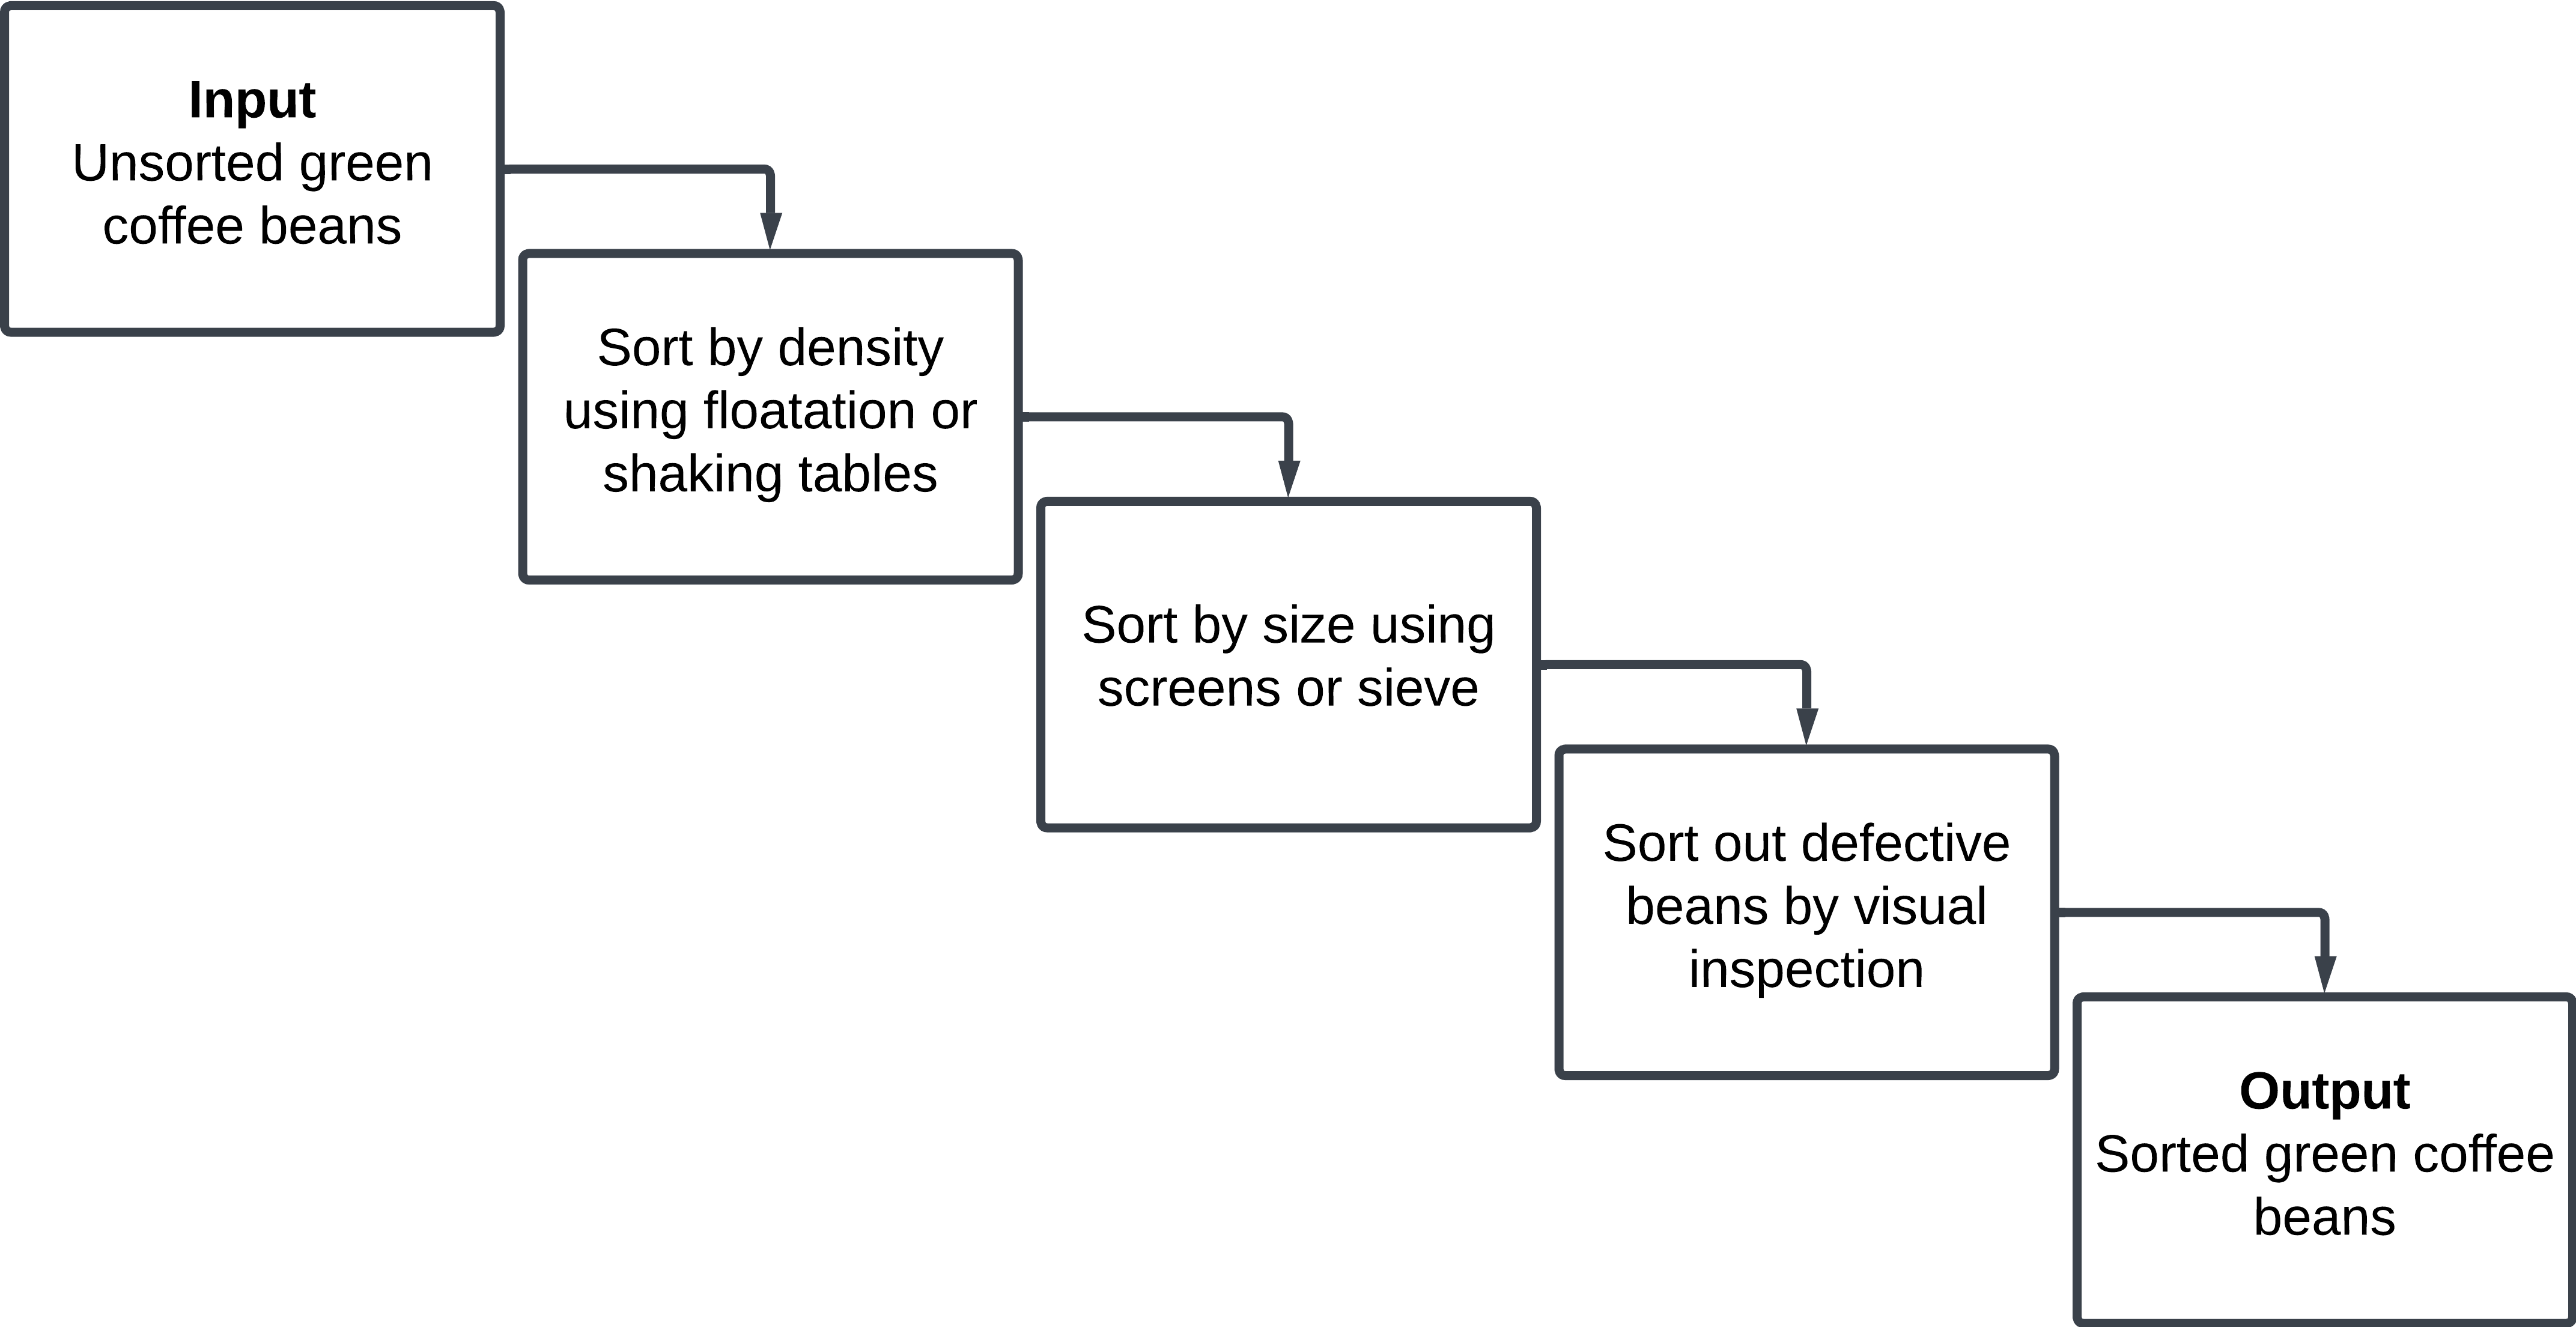
\includegraphics[width=0.9\textwidth]{figure/manual_sorting.png} 
\end{center}

The diagram in Figure 1 depicts the representation of the process of manual sorting of unsorted green coffee beans through a series of steps. First, the beans are sorted by density using methods such as floatation or shaking tables. This helps in separating the denser beans, usually pertaining to a more developed and higher quality bean. Then, the beans are sorted by size using screens and sieves with specific dimensions depending on the variety of the beans. After this, a thorough visual inspection is performed by the sorters to identify and remove the defective beans from the batch. The visual inspection includes sorting out cracks, discoloration, undeveloped and other defective bean characteristics. Finally, the process results in the output of sorted green coffee beans, ready for further processing or sale. 

\subsection{Description of the System}

\includegraphics[width=0.9\textwidth]{figure/placeholder.png} 

The proposed system is a two-staged automated green coffeee bean sorting machine, integrating both machine vision and density analysis. Firstly, the coffee beans are introduced into the system through a funnel, which directs them to a conveyor belt mechanism.  In the first stage, the green coffee beans will be sorted depending on their visual characteristics. In this stage, the physical qualities of the bean is analyzed such as size, color, and defect. If the bean is defective, the system will automatically sort it out. Then, all the non-defective beans will go through the second stage of the system. In the second stage, there will be an IR sensor and a weighing scale. The IR sensor will help the system to calculate for the estimated volume of the bean. The volume and mass of the bean in hand, the density of the bean can be calculated. Depending on the density threshold and size threshold set by the user, the bean will be classified whether it is good or not.


\includegraphics[width=0.9\textwidth]{figure/placeholder.png} 

Figure 3 shows the schematic diagram of the proposed system. Arduino Uno microcontroller magaes all the mechanical components such as the servo motor, stepper motors, and the converyor belt. The servo motor controls the  roitating mechanism for bean sorting. On the other hand, the stepper motors operate a slide mechanism to direct the beans. Two cameras, integrated with OpenCV via Python, handle machine vision algorithms, and image processing for defect detection of the beans. A ToF10120 sensor provides precise distance measurement. A precision weighing scale measures the density of each bean for classification. The Arduino communicates with the OpenCV system through serial communication, ensuring smooth coordination.


\includegraphics[width=0.9\textwidth]{figure/placeholder.png} 

Figure 4 shows the design overview of the system. Beans are first arranged through a hopper and a conveyor belt. On top of the conveyor belt, a 3D-printed guide is attached for the beans to maintain a linear formation. Then, the beans are expected to fall into another funnel attached to a tube. The tube is directly attached to a rotating mechanism that allows the beans to be inspected and sorted one-by-one. In this stage, defective beans are sorted out. Then, the non-defective beans are transferred onto the precision scale to analyze the density. The less-dense beans are sorted out of the batch.


\includegraphics[width=0.9\textwidth]{figure/placeholder.png} 

\subsection{Dataset and Model Training}
For the dataset collection, Arabica specialty-grade green beans from a farm will be used. Each bean is expected to be captured by a high-resolution camera with sufficient lighting. The top and bottom side pictures of the beans are to be collected. In addition, defective beans of the same type and origin will be gathered to identify the different classification of defects (primary and secondary). In this study, all primary defects are considered such as Full Black, Full Sour, Dried Cherry, Fungus Damage, and Severe Insect Damage. On the other hand, secondary defects are also considered such as Partial Black, Parchment, Floater, Shell, and Chipped. For the dataset collection, at least 500 images of good beans and at least 200 beans for each defect classification will be gathered to train the model. To further improve and increaase the dataset size, augmentation will be applied by scaling, rotating, and mirroring the images. 

The models to be used in this study are Convolutional Neural Network (CNN) and Random Forest. The CNN model is mostly compatible for image classification and feature extraction as it is composed of several different layers resulting in a better representation of image data (Wang et al., 2021). Thus, this model is the most ideal for green bean defect detection by identifying its texture, color, size, volume, deformations, and cracks in the first stage of sorting. Then, for the second stage where density parameter is added, Random Forest will be used. Since mixed data types are being considered (visual features extracted by CNN and density values), Random Forest is the best fit for this classification (Rigatti, 2017). In addition, the model is robust to overfitting, which means that it can handle noisy data. 

\subsection{Testing}
For the testing procedures, processed but unsorted green coffee beans will be acquired from a local farmer. These coffee beans will be sorted manually based on their different defects and quality, and also will be fed into the automated system to compare accuracy and performance. In line with the Philippine National Standard  or PNS (2022) for testing green coffee bean sorters, three test trials will be conducted. These trials will be conducted under similar operational settinsg to ensure consistency. The duration of each trial begins when the beans are fed into the system’s hopper and endsd after no beans remain in the system. During these trials, the system’s ability to sort defective beans and categorize the good beans by density will be monitored.
To create the dataset, coffee beans will be arranged on a sheet of paper and photo of the entire sheet will be taken. A program using YOLOv8 will then be used to process this image, detecting each bean, creating bounding boxes, and crop them into separate image files for labeling. Additionally, an alternative method involves using the system itself to collect data, with cameras capturing the top and bottom of the beans as they pass through the system. These approaches aim to ensure to create a diverse dataset that will be used for training the machine learning model.

In evaluating the system’s performance, various metrics, as dictated by the PNS for Green Coffee Bean Sorters, will be considered: 
\begin{itemize}
	\item \textbf{Sorting Accuracy}. The system’s sorting accuracy will be verified by comparing the output of the system to the manually sorted output of the same batch of beans.
	\item \textbf{Duration of Tests}. The total operating time for each trial will be recorded.
	\item \textbf{Sorting Yield}. The quantity and quality of the beans sorted in each trial will be measured to assess the system.
\end{itemize}


The desired accuracy of the system for its defect sorting is an accuracy of at least 85\%. The paper of Lualhati et al. (2022) was able to achieve an accuracy score of 85\% for sorting out good beans and 95\% for defect sorting, with an average score of 90\% for sorting out both. However, their paper only included two types of defects (black and deformed), and good quality beans as its data set. This study aims to target 10 types of defects along with the good green coffee beans ensuring that the system can cover a wider range of defects while also matching the accuracy of the previous study. 

To validate the performance of the system, the results will be compared with those obtained during the manual sorting. This comparison will focus on determining the accuracy of the defect detection and bean classification. The manual sorting process will serve as the reference for evaluating the system’s ability to enhance sorting efficiency and accuracy.

\subsection{Graphical User Interface (GUI)}
The proposed system would be integrating a graphical user interface developed using PyGui and ChatGPT API. The GUI would serve as the control center platform for the system. This would provide real-time feedback and insights for users. As shown in Figure 8, a concept of how the GUI would interact with the system would be a start button, once the button is executed the system would then be expecting inputs and start sorting. There would be real-time feedback during the sorting process, then some visual markers to indicate their classification, and an elapsed time so the user would be aware of the time of the sorting process. Once the system is done, the user can click the end button and the summary report would generate in an orderly manner, providing tables of classification that was detected through the process. In the bottom part of the GUI, ChatGPT API would be integrated and would offer recommendations based on the detected quality and classification of the coffee beans. 

\ifFinished
\else

\section{Estimated Work Schedule and Budget}

The estimated work schedule can be represented as a Gantt Chart or a combination of Project Network Diagram, Work Breakdown Structure, and Critical Path.  The budget can be made into a Bill of Materials, financial plan, or if your \documentType \ is funded and part of larger project, the cost, and date for reaching each milestone and/or deliverable for your part of the project.

For ECE Department undergraduate theses, the individual Gantt Chart or Work Breakdown Schedule and Bill of Materials will be included in this section and be removed in the final document.

\graytx{\blindtext}

\ifPhD
\section{Publication Plan}
\graytx{\blindtext}
\fi

\fi


\section{Overview of the \documentType}

Provide here a brief summary and what the reader should expect from each succeeding chapter.  Show how each chapter is connected with each other.


	%\stopcontents[chapters]
	\cleardoublepage
	
	%%%%%%%%%%%%%%%%%%%%%%%%%%%%%%%%%%%%%%%%%%%%%%%%
	\chapter{Literature Review} 
	\label{ch:litrev} 
	%\startcontents[chapters]
	%\begin{SingleSpace}	
	%	\Mprintcontents 
	%\end{SingleSpace}
	It is to be noted that each subsection in this chapter should discuss in narrative form each table that is presented in order to point out to the reader what the author(s) intend to convey.

\section{Existing Work}

Cite and summarize here relevant and significant literature (dissertations, theses, journals, patents, notable conference papers) through a table and descriptions to prove that no one has done your work yet and/or that your work is not a duplication of existing ones. Your focus here is what has \emph{been done}.

\graytx{\Blindtext}

\section{Lacking in the Approaches}

You can summarize the weaknesses of existing approaches by a tabular comparison of the literature. Your focus here is what has \emph{not been done}, i.e. what features were missed, what solutions were not considered, what the demerits are, etc.  Through these items, you then can introduce the necessity for doing your proposed solution.  

It is to be noted that the degree of novelty for undergraduate thesis is lower than those for graduate school. If a Ph.D. dissertation/thesis has a high degree of novelty and that for an undergraduate is low, then a master's thesis is somewhere between the two.

Briefly include here the following in order to remind the reader why you are highlighting the weaknesses of the solutions of existing literature. 

\begin{itemize}
	\item mentioning the problem
	\item showing how your solution is better (can be better (for proposals))
\end{itemize}


\graytx{\Blindtext}

\section{Summary}

Provide the gist of this chapter such that it reflects the contents and the message.





	%\stopcontents[chapters]
	\cleardoublepage
	
	%%%%%%%%%%%%%%%%%%%%%%%%%%%%%%%%%%%%%%%%%%%%%%%%
	\chapter{Theoretical Considerations}
	%\chaptermark{Theoretical Considerations} % uncomment this and put a shorter version of the chapter title for the TOC and chapter markings (i.e., header or footer)
	\label{ch:theorycon}
	%\startcontents[chapters]
	%\begin{SingleSpace}	
	%	\Mprintcontents 
	%\end{SingleSpace}
	

\section{Theoretical Framework}

\begin{figure}[!htbp]
	\centering
		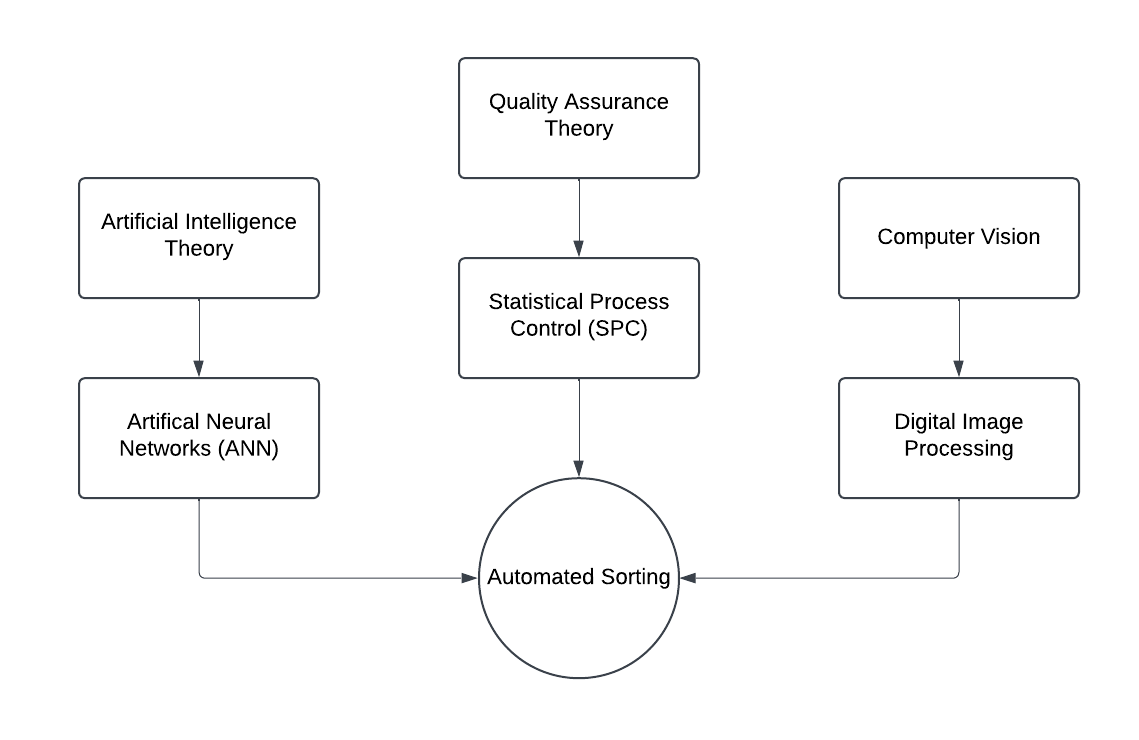
\includegraphics[width=0.8\textwidth]{figure/theoretical_framework.png}
	\caption{Theoretical Framework}
	\label{fig:theoretical_framework}
\end{figure}

The theoretical framework discusses the multiple concepts that are involved in this study. These key concepts are crucial to ensuring the success of the thesis. There are three main concepts that are key to this study, the Artificial Intelligence Theory, the Quality Assurance Theory and lastly, Computer Vision.

\section{Conceptual Framework}

\begin{figure}[!htbp]
	\centering
		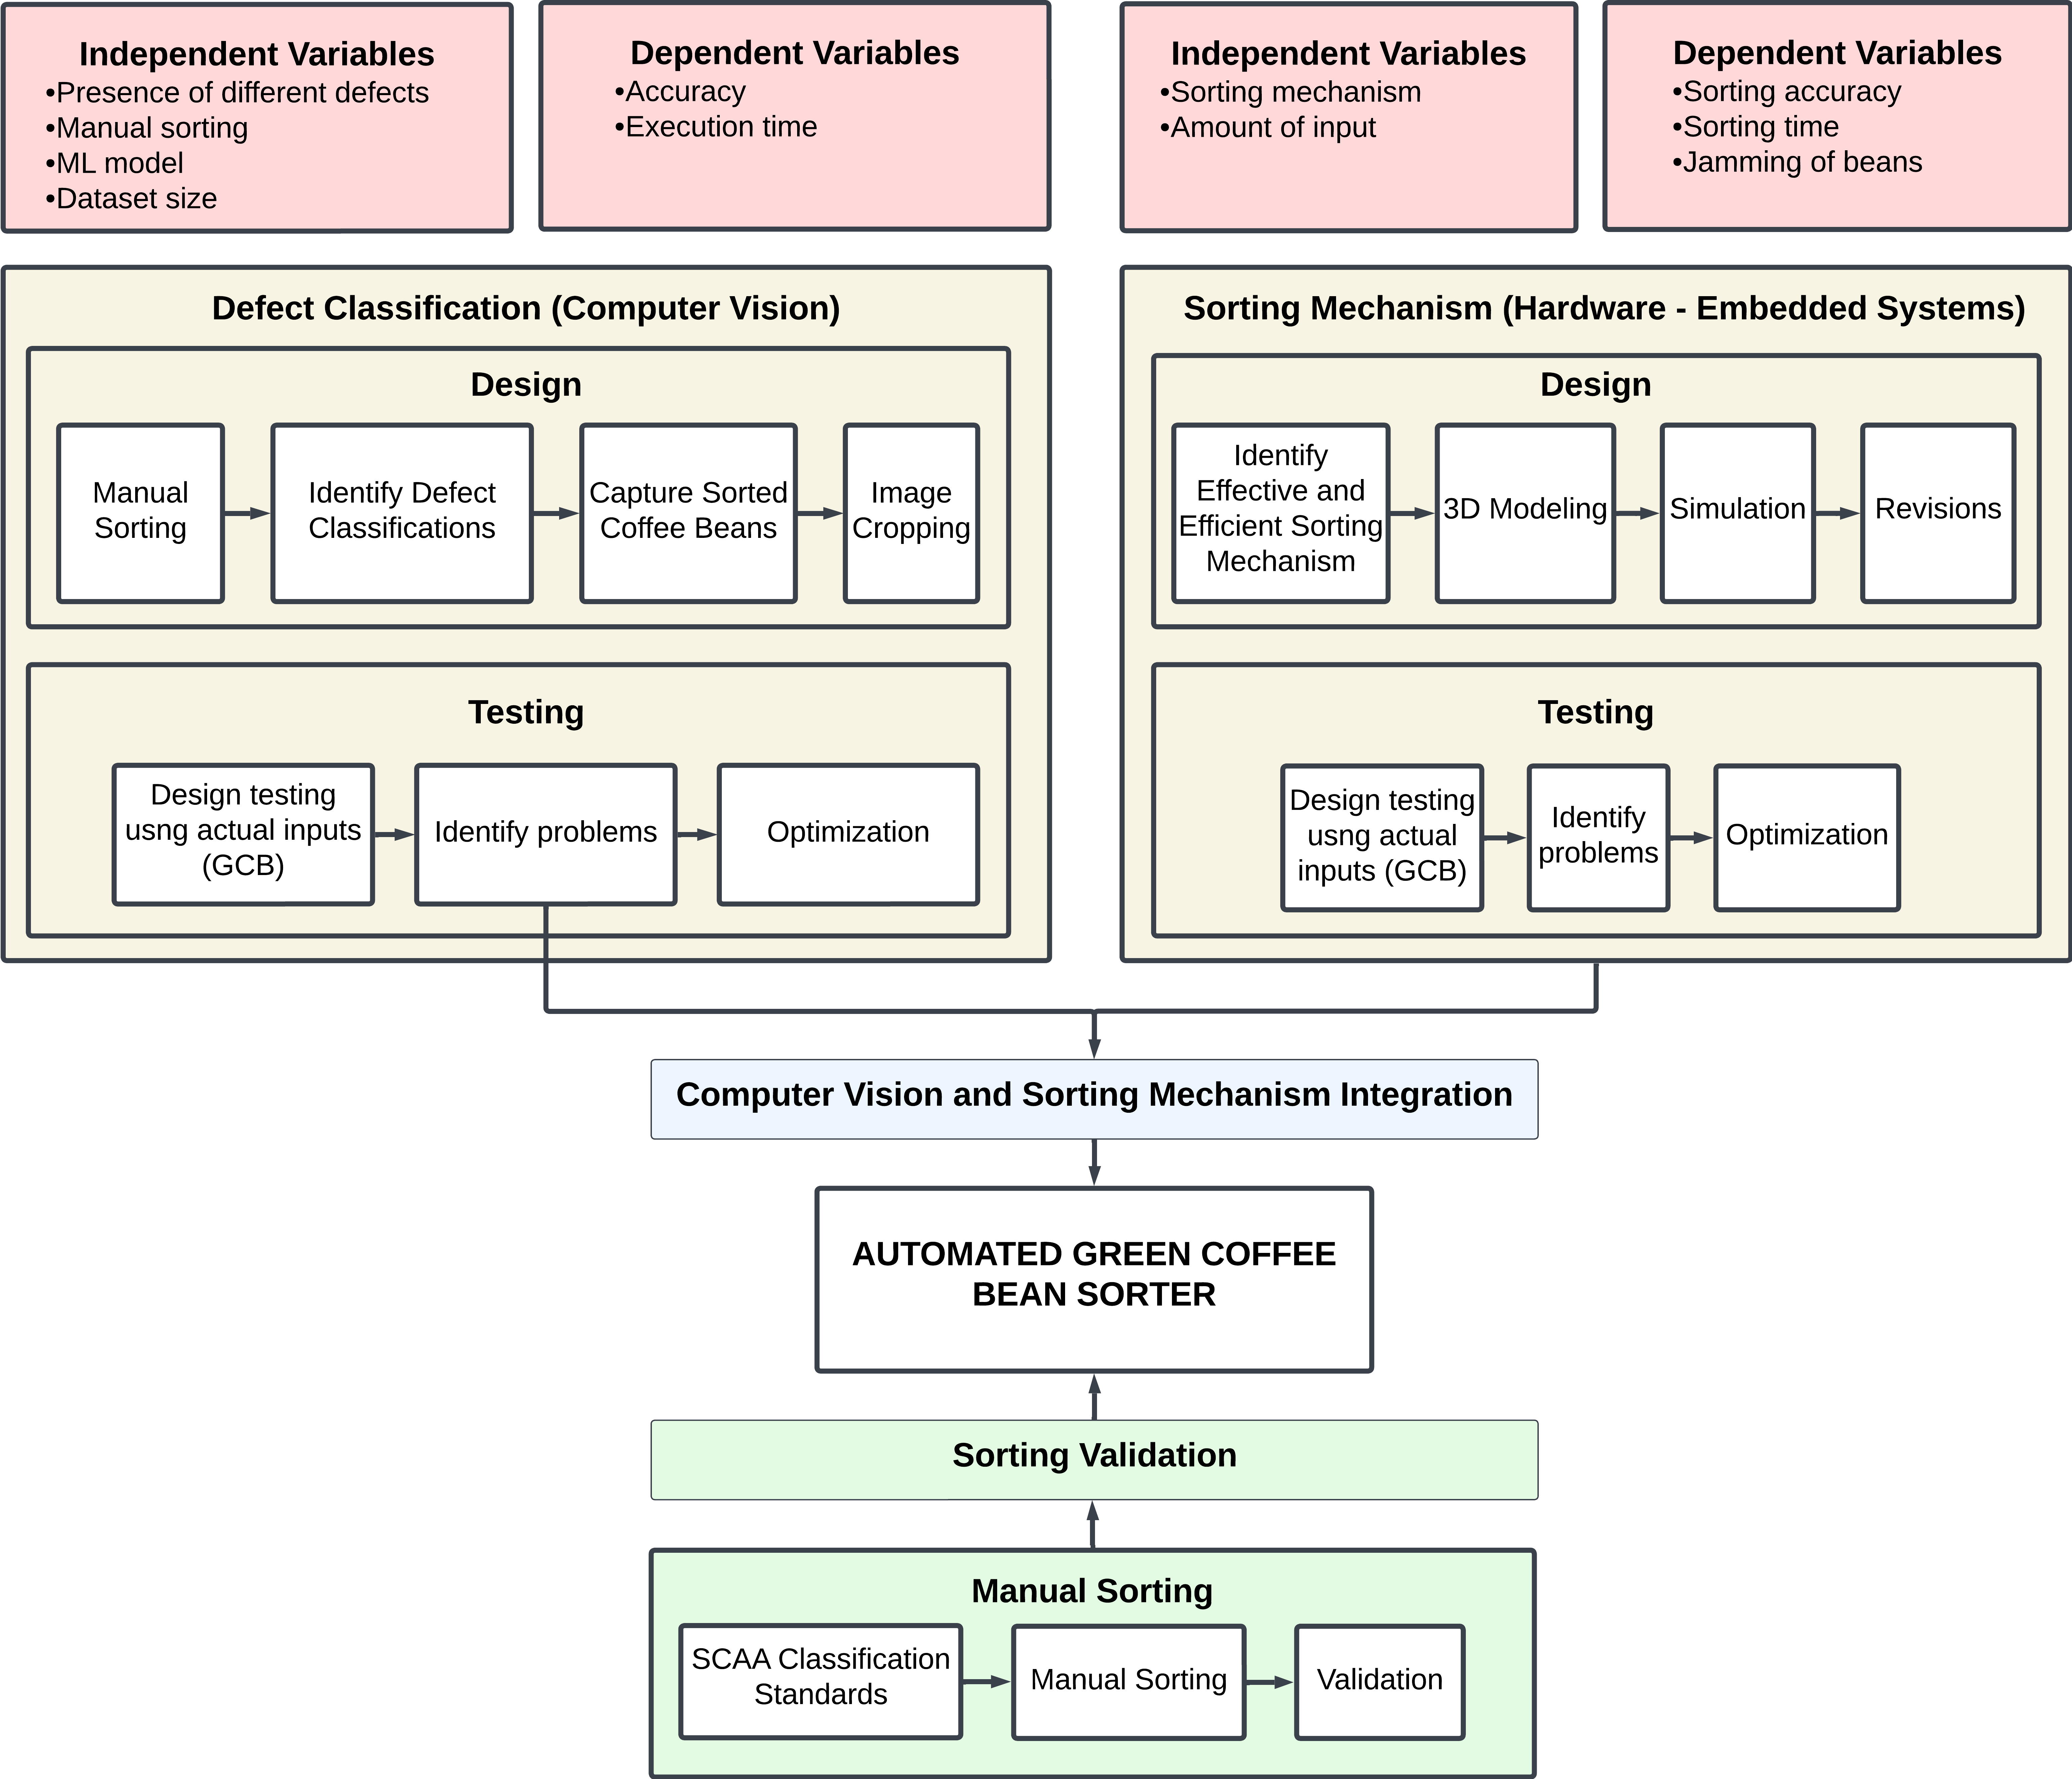
\includegraphics[width=\textwidth]{figure/conceptual_framework_v2.png}
	\caption{Conceptual Framework}
	\label{fig:conceptual_framework}
\end{figure}

The conceptual framework shows the implementation of two systems which consists of machine vision and embedded systems. The framework describes the thought process of both systems with the end goal of integrating both systems. The machine vision handles the defect classification of the system, whereas the embedded system handles the sorting of the beans. By integrating both systems together, creates an automated green coffee bean sorter. The data validation is done by sorting through the tested coffee beans by the system following the standards of the SCAA.

\section{Quality Assurance Theory}
Quality assurance theory refers to the set of principles and practices that focuses on establishing a systematic process to ensure that a product or service conforms to a predetermined standard. In the aspect of food and agriculture, there are a number of practices and principles that ensure the safety and quality of food products. According to \cite{da_Cruz_Cenci_Maia_2006}, there are a number of practices in place that must be followed, one of which is Good Agricultural Practices, where these procedures are aimed to reduce hazards related to product safety at the farm level. Another one of said practices is the Good manufacturing practice, which were formerly called support programs that provide foundations to the overall food safety management programme. This includes cleaning, maintenance, personnel training, calibration equipment, quality control, and  pest control. Industries that adopt such practices produce the following results, better quality products, greener initiatives and better productivity within a department. Lastly, hazard analysis and critical control points (HACCP), is a science-based system that was created to identify potential hazards and actions to control said hazards. This practice is used to ensure food safety. 

In the context of coffee beans, there are a number of systems in place to ensure that quality beans are being provided to the consumer market. The governing body known as the Specialty Coffee Association (SCAA) has implemented grades to green coffee beans to provide a better way to classify said beans. These grades can be differentiated into 5 grades namely, Specialty Grade, Premium Coffee Grade, Exchange Coffee Grade, Below Standard Coffee Grade, and Off grade Coffee. They are classified according to the number of defects found in a sample batch of 300 grams and according to their size. Specialty grade coffee beans are supposed to contain less than 5 defects in a sample batch while also not allowing any primary defects to be present; it should only have less than 5\% difference between its sizes. Coffee beans in this grade should also contain a special attribute whether in its body, flavor, aroma, or acidity, and its moisture content should only be in the range of 9-13\%. Premium Coffee grade beans should only contain 8 full defects in a sample batch but primary defects are allowed in the sample batch. Similarly to specialty grade coffee beans, its sizes should only contain a 5\% difference to one another; it should also contain a special attribute and moisture content should also be similar to its specialty grade counterpart. Exchange coffee grade should contain defects ranging from 9-23 beans in a sample batch, with sizes that can vary up to 50\% difference in weight but also only 5\% in its sizes. Below standard and off grade coffee beans are classified according to the number of defects present in a sample batch; 24-86 beans for below standard while more than 86 beans for off grade. These gradings are used to ensure that quality green coffee beans are produced and ensure that consumers are provided with the best quality available. 

\section{Artificial Intelligence Theory}

Artificial Intelligence in defect classification are widely used in this industry which are commonly used in manufacturing and industrial applications. Several deep learning techniques are used in order to achieve an effective defect classification. Models such as convolutional neural networks (CNNs)  and You Only Look Once (YOLO) are widely used for classification. CNN utilizes an image based analysis and feature extraction approach to identify different classifications. CNN is more effective in analyzing grid-like data like images, making it suitable for defect classification \cite{Das_Hollander_Suliman_2019}. One of its major advantages is its ability to automatically detect important features such as shape, patterns, and edges. Although it may have its own advantages, there are also disadvantages that need to be taken into account, mainly in scenarios that involve class imbalance and complex backgrounds (Moon, 2021) . YOLO is another model that is suitable for defect classification, its ability to provide real-time defect classification while also providing high accuracy is essential in some industries. In YOLO, there are several versions that are developed over the years, which are supposed to bring several improvements in terms of speed, accuracy, and computational efficiency. Combining different models is also effective, in the case of \cite{Deepti_Prabadevi_2024}, they combined transformer architecture with YOLOv7 to enhance its feature extraction, this resulted in an increase of 5.4\% in mean average precision and F1 score. 

\section{Computer Vision Theory}

There are fundamental concepts that need to be done for image processing in detection. There are pre-processing techniques like preprocessing and segmentation. Pre-processing is a general term for preparing an image to be analyzed by the system, this includes techniques such as denoising an image, applying filters, and enhancing the image to further improve the visibility of defects \cite{Lee_Tai_2020} . Segmentation is dividing the images into segments to make the analysis simpler, methods such as histogram segmentation and active contour models helps in isolating the regions of interest. 

For defect classification, feature extraction is important to identify the relevant features then extracting said features to to help indicate specific defects, this utilizes the edges, textures, and shapes to help in defect classification \cite{Wu_Hao_Song_2024}.  By utilizing OpenCV and deep learning models is advisable for automatic feature extraction. Models like CNN, can automatically extract features from images, which greatly reduces the need for manual extraction, this helps in a more robust and scalable solution \cite{Bali_Tyagi_2020}. The versatility of OpenCV library which allows support for multiple image pre-processing tasks, when combined with deep learning models can be applied to different fields. 

\section{Performance Evaluation}

Accuracy, precision, recall, and F1 score are common measures to assess how well classification models predict. Accuracy measures how good a model is by computing the ratio of correct predictions to all predictions. While appropriate for balanced datasets, accuracy can be deceptive when dealing with imbalanced classes, since a model can be very accurate by predicting the majority class. Precision measures how well positive predictions are obtained by calculating the number of correct predicted positive instances. This is particularly important  when false positives are costly, such as in the case of spam. Recall, or sensitivity, measures how well a model identifies true positive instances, which is very important in cases where failing to detect a positive instance is costly, such as in medical diagnosis. Since precision and recall trade off each other, the F1 score reconciles the two by computing their harmonic mean. This measure is particularly appropriate when a trade-off between precision and recall is desired, so that neither false positives nor false negatives dominate the assessment. In general, these measures provide a general impression of how good a model is and help decide how well-suited the model is for different applications.

\section{Existing Technologies and Approaches}
The paper done by \cite{Lualhati_Mariano_Torres_Fenol_2022}, is a green coffee bean sorter that utilizes MATLAB as its image processing. The system created uses a PID based algorithm and image processing algorithm for sorting. The system utilized two cameras to capture both sides of the bean. The system of Lualhati et al. comprises only 3 green coffee bean classifications, which are good, black and deformed coffee beans. The developed system uses multiple stepper motors for the defect sorting, while 2 cameras were used to handle the green coffee bean detection. 

The paper of \cite{Balay_Cabrera_Jensen_Mayuga_2024}, is an automatic sorting for green coffee beans utilizing computer vision and machine learning for defect classification. The system developed uses the YOLOv8 model alongside a Raspberry Pi based image processing to identify and classify the green coffee beans. The defects that the group classified are full black, partial black, chipped, dried cherry, shell, and insect damage. The system developed uses a conveyor belt and sorting motor for an automated defect separation. They used one camera module, the raspberry pi camera module 3 NoIR for the defect detection of the system. 

The study of \cite{Muchtar_Hafifah_Febriana_Dawood_Ahmadiar_Bahri_Lin_Yohannes_2025} explored the use of 9 image classification models with varying architectures such as CNN-based (EfficientNetB7, DenseNet121, InceptionV4, etc.)  and Transformer-based models (ViT, Swin Transformer, FocalNet, etc.) in detecting defective coffee beans. The study focuses on differentiating defective from good coffee beans, but doesn’t distinguish between defects. The results of the study suggest that FocalNet outperforms all other models significantly in both training and testing phases for detecting defects in coffee beans.


\section{Density Measurement}
In measuring the density of the coffee bean there are a number ways this can be done, one way is by measuring the bulk density of the batch. This is done by measuring the mass of a batch then dividing it to a fixed volume. The more appropriate method for measuring the density of the coffee bean is called “free settle” density or free-flow density. This is defined as the ratio of the mass of the coffee beans to the volume they occupy after being allowed to flow freely into a container. It is expressed in grams per liter or kilograms per cubic meter. 

\begin{equation}
	d = \frac{m_2-m_1}{V}
\end{equation}

where $m_2$ is the mass of the green coffee bean, $m_1$ is the mass of the empty container, and $V$ is the capacity (in liters) of the container \cite{International_Organization_for_Standardization_1995}.

\section{Summary}
This chapter gives the theoretical and conceptual backgrounds of an automated green coffee bean sorter using Artificial Intelligence (AI), Quality Assurance, and Computer Vision. The theoretical background focuses on key concepts like deep learning models (CNNs, YOLO, ViT) used for defect classification, quality assurance principles (GAP, GMP, HACCP) ensuring food safety, and computer vision algorithms (preprocessing, segmentation, and feature extraction) used for image analysis. The conceptual background explains the integration of machine vision for defect detection with embedded systems for sorting, thus conforming to the SCAA coffee grading standards. Performance metrics like accuracy, precision, recall, and F1 score are used for evaluating the performance of the model. Current technologies, for instance, those of \cite{Lualhati_Mariano_Torres_Fenol_2022} and \cite{Balay_Cabrera_Jensen_Mayuga_2024}, provide insights relevant to image processing and machine learning-based sorting techniques, thus contributing to automated coffee bean classification development.

	%\stopcontents[chapters]
	\cleardoublepage
	
	%%%%%%%%%%%%%%%%%%%%%%%%%%%%%%%%%%%%%%%%%%%%%%%%
	\chapter{Design Considerations} 
	\label{ch:designcon} 
	%\startcontents[chapters]
	%\begin{SingleSpace}	
	%	\Mprintcontents 
	%\end{SingleSpace}
	\section{Mechanical Design}

\subsection{Screw Feeder}
% TODO: FIX Citation and Picture
\begin{figure}[h]
\centering
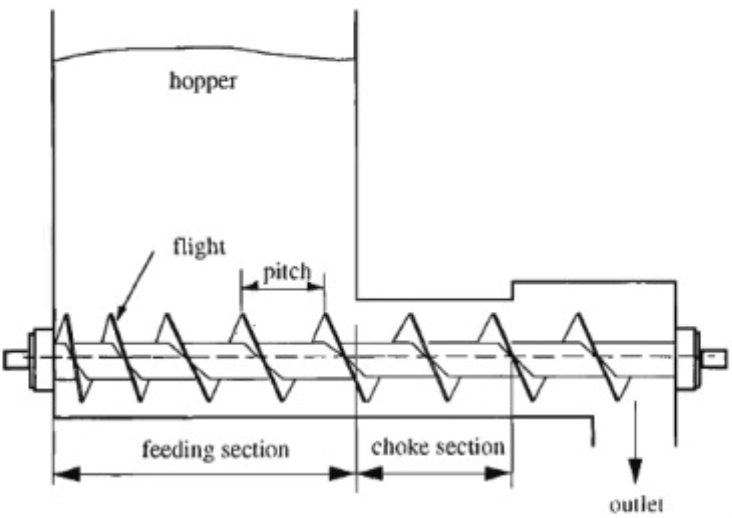
\includegraphics[width=6cm]{ch4/Screw_Feeder_Diagram.png} % replace with image path
\caption{Screw Feeder Diagram}
\label{fig:screw_feeder_diagram}
\end{figure}

% TODO: Update Citation
Figure \ref{fig:screw_feeder_diagram} shows the diagram of a screw feeder. Screw feeders are usually used in industrial fields like agriculture, chemicals, plastics, cements, poultry and food processing. According to \cite{Minglani_Sharma_Pandey_Dayal_Joshi_Subramaniam_2020}, screw feeders are specifically used to transport or move granular materials at a controlled rate like corn and wheat. It consists of a rotating screw and small feeding section or the hopper. Despite having big batches of a certain material, screw feeders can control the rate of which these materials are dispensed. With this concept, the group decided to utilize a screw feeder as the input mechanism for the system. This mechanism allows a controlled rate of coffee bean dispensing, which is a significant factor to avoid overcrowding in the rotating conveyor table causing the beans to jam. In addition, batches of coffee beans can be put at once instead of just adding a certain amount of beans at a time. 

\subsection{Rotating Conveyor Table}
\begin{figure}[h]
    \centering
    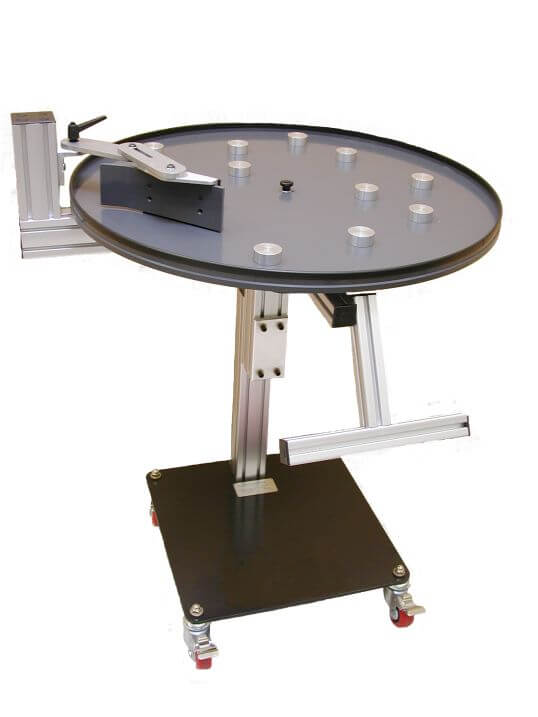
\includegraphics[width=6cm]{ch4/rotating_conveyor_table.jpg} % replace with image path
    \caption{Rotating Conveyor Table 3D Design, 32-inch Rotary Table Accumulator (RTA)}
    \label{fig:rotating_conveyor_table}
\end{figure}

After the inputted beans comes out from the screw feeder, the coffee beans would then be placed in the rotating conveyor table. According to the study of \cite{Dabek_Krot_Wodecki_Zimroz_Szrek_Zimroz_2022}. The conveyor table is used as a transportation systems for all forms of bulk materials to a certain machine or destination. The system utilizes the rotating conveyor table to have a controlled movement of coffee beans towards the first stage of the system. The improvised linearization system, consisting of metal guide rails and dividers ensures that beans align in a single path, reducing random movement, and improving the flow of the input beans. An infrared sensor would detect each bean as it passes, to control the movement of the bean preventing clogging and ensuring efficient operation. 

\subsection{Inspection Tray (1st Stage)}

\begin{figure}[h]
    \centering
    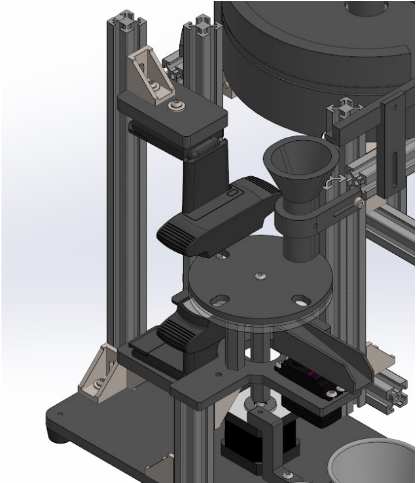
\includegraphics[width=6cm]{ch4/Inspection_Tray_3D_Design.png} % replace with image path
    \caption{Inspector Tray 3D Design}
    \label{fig:inspection_tray}
\end{figure}

The inspection tray serves as the platform for the machine vision based analysis of coffee beans. It is designed with 8 holes, allowing uniform placements and optimal camera positioning for the system. The system utilizes a two-layer structure: a stationary acrylic platform and a rotating 3D-printed platform with holes. The rotating mechanism sequentially positions each bean between two webcams, which captures and analyzes its physical characteristics from top and bottom perspective. This design captures both sides of the bean, ensuring a better classification of the bean. After inspection, the bean moves onto a slide, where it is either directed to the second stage for density analysis (Good) or sorted out as a defect.

\subsection{Density Sorter (2nd Stage)}

In measuring the density of the coffee bean there are a number ways this can be done, one way is by measuring the bulk density of the batch. This is done by measuring the mass of a batch then dividing it to a fixed volume. The more appropriate method for measuring the density of the coffee bean is called “free settle” density or free-flow density. This is defined as the ratio of the mass of the coffee beans to the volume they occupy after being allowed to flow freely into a container. It is expressed in grams per liter or kilograms per cubic meter. 

\section{Embedded Systems}

\subsection{Microcontroller}

\begin{figure}[H]
    \centering
    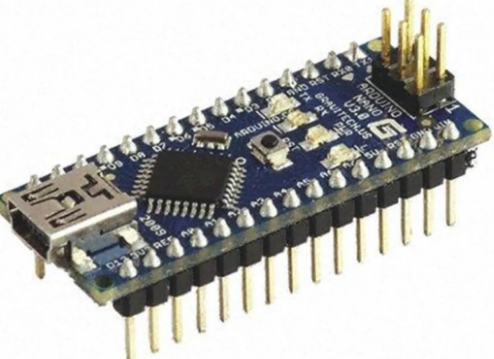
\includegraphics[width=6cm]{ch4/Arduino_Nano_Microcontroller.png} % replace with image path
    \caption{Arduino Nano Microcontroller}
    \label{fig:arduino_nano}
\end{figure}

Since the system is composed of two stages of sorting: defect sorting through computer vision and density-based analysis–the group decided to utilize two Arduino Nano microcontrollers to modularize the control process. The first Arduino Nano microcontroller is tasked to handle the computer vision-based defect sorting through serial communication with OpenCv operating in Python. In addition, it handles the operation of defect sorting consisting of a stepper motor for the rotation of the inspection tray and a servo motor for the slider, which directs the beans to the designated bin (defect or good bin). On the other hand, the second Arduino Nano microcontroller manages the density-based analysis and sorting, which consists of another stepper motor to direct the beans to its respective bin (dense and less-dense bin), the precision scale which is interfaced through RS232, and the top feeder where the input beans are poured. The use of separate Arduino microcontrollers is advantageous when it comes to the computer vision-based sorting of beans. This is because serial communication is much faster when code complexity is significantly reduced. With this, a designated microcontroller handles the computer vision part and two-way serial communication between the microcontroller and the computer vision algorithm running in Python. Most importantly, the use of two microcontrollers allowed the system to not rely solely on a sequential approach. This means that the two stages of sorting are not relying on the timing of each other, allowing the inspection tray and the top feeder to operate independently. Thus, resulting in a much faster and efficient sorting process. 

\subsection{Sensors}

\begin{figure}[H]
    \centering
    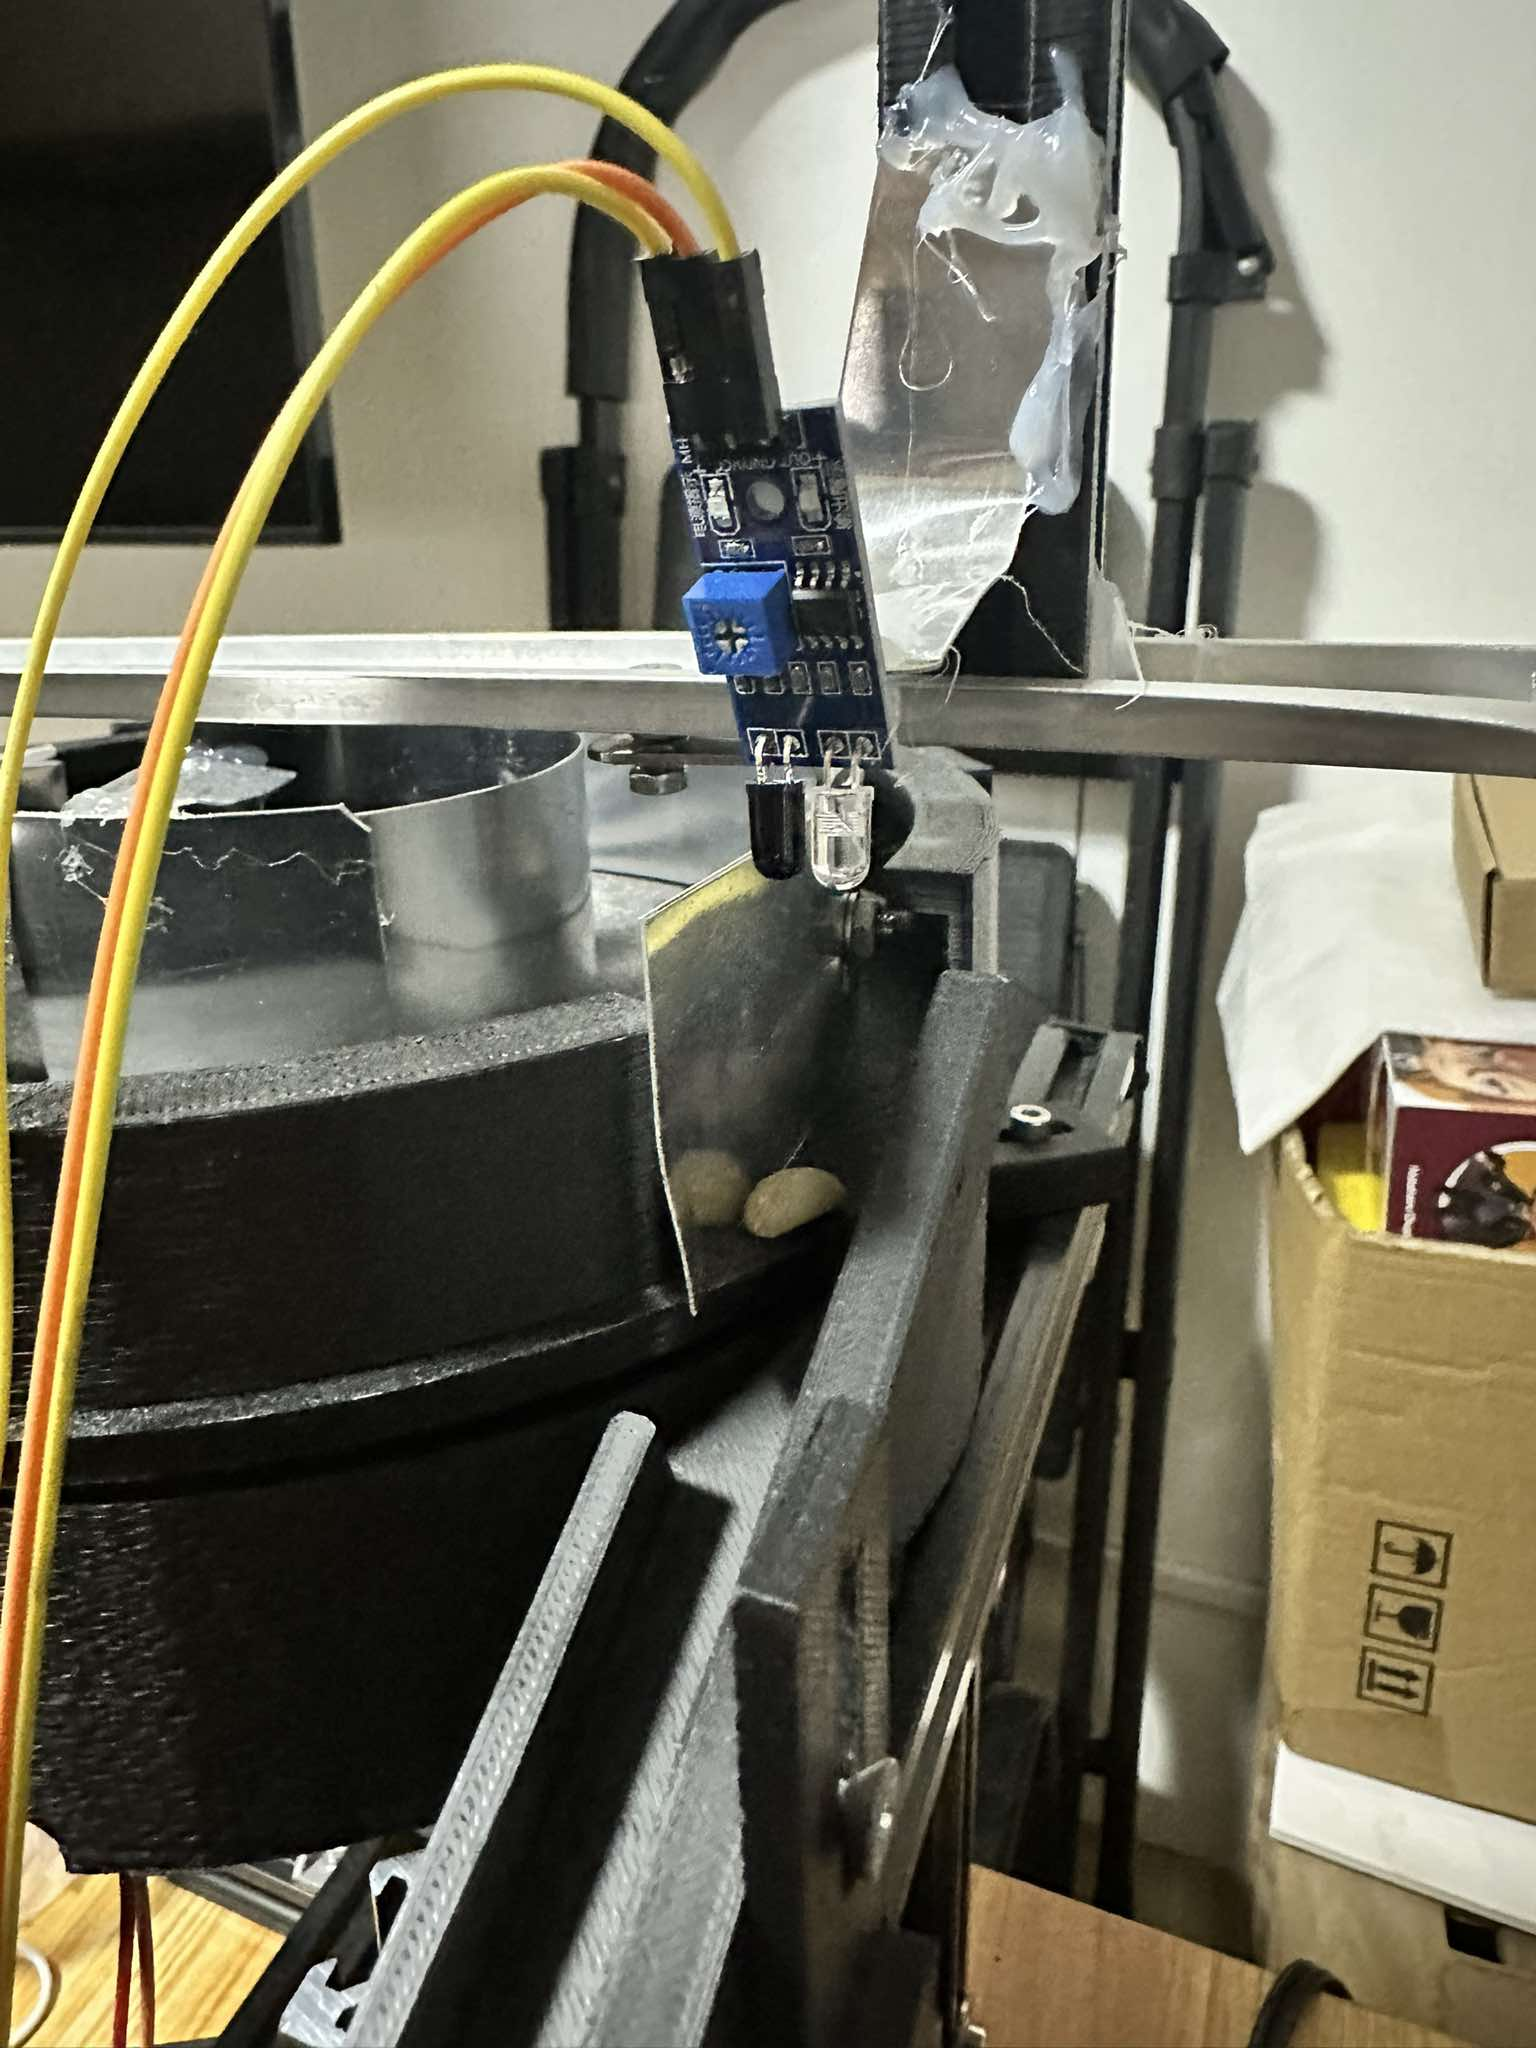
\includegraphics[width=6cm]{ch4/Infrared_Sensor.jpg} % replace with image path
    \caption{Infrared Sensor}
    \label{fig:infrared_sensor}
\end{figure}

To ensure that the beans are falling in a one-by-one manner onto the inspection tray, the group placed an IR sensor at the edge of the top feeder. This IR sensor triggers the DC motor that runs the feeder to stop, and runs small steps until the bean is dropped. The addition of the IR sensor at the edge of the feeder allows the motor to run continuously until another bean is detected. With this, the waiting time for the next bean at the inspection tray is significantly lessened. 

\begin{figure}[H]
    \centering
    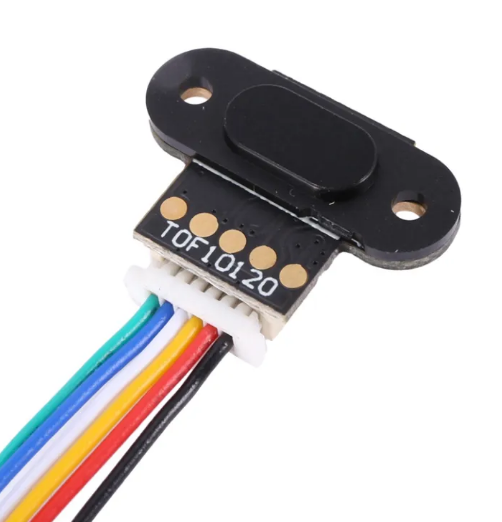
\includegraphics[width=6cm]{ch4/TOF10120.png} % replace with image path
    \caption{TOF10120}
    \label{fig:tof10120}
\end{figure}

TOF10120 or Time of Flight sensor is utilized in the system due to its high precision, non-contact measurement capability. This sensor is used to estimate the volume of each bean, which is essential for computing the density. In the second stage of sorting, where beans are classified based on density, the sensor plays a crucial role in determining the approximate volume of each bean by measuring its height or dimensions as it passes through the system.

\subsection{Motor control}

\begin{figure}[H]
    \centering
    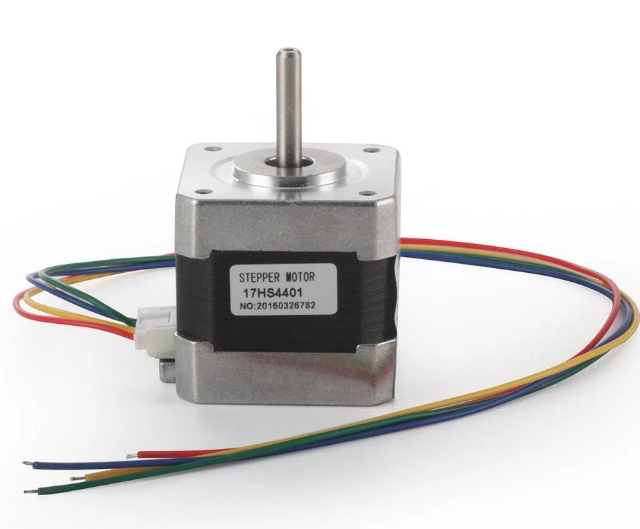
\includegraphics[width=6cm]{ch4/12V_NEMA_17_Stepper_Motor.png} % replace with image path
    \caption{12V NEMA 17 Stepper Motor}
    \label{fig:stepper_motor}
\end{figure}

Two NEMA 17 12V stepper motors, paired with L298N motor drivers were used to control the movement of the inspection tray in the first stage and the density-based sorting mechanisms in the second stage. In these mechanisms, the group decided to use stepper motors to ensure precise and accurate movements. Precise and accurate movements are needed for the inspection tray to make sure every movement of the hole is perfectly aligned to the camera. Thus, allowing a more uniform and consistent angle for each bean to be inspected through the computer vision. In addition, NEMA 17 stepper motors were the best choice for these mechanisms due to its high torque, which is essential because it will be moving weighted objects. 

\begin{figure}[H]
    \centering
    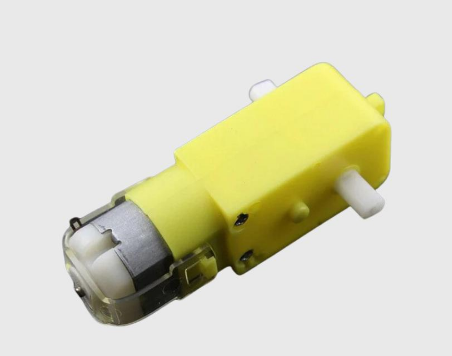
\includegraphics[width=6cm]{ch4/6V_DC_Motor.png} % replace with image path
    \caption{6V DC Motor}
    \label{fig:6v_dc_motor}
\end{figure}

For the rotating conveyor table (top feeder), where the beans are initially poured, a 6V DC motor is used. The group decided to use this motor due to its high RPM, which is needed for a fast rotation of the rotating conveyor table. The speed of the feeder is regulated to prevent clogging and ensure that the beans are evenly spaced before they enter the inspection tray. The motor speed is fine-tuned through pulse-width modulation (PWM) to synchronize with the stepper motor-driven inspection tray, ensuring a steady input without overwhelming the system.

\begin{figure}[H]
    \centering
    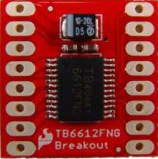
\includegraphics[width=6cm]{ch4/TB6612FNG_Motor_Driver.png} % replace with image path
    \caption{TB6612FNG Motor Driver}
    \label{fig:motor_driver}
\end{figure}

To drive the 6V DC motor, the group utilized TB6612FNG, a motor driver module. This module also allowed PWM control for the motor, which is essential for reducing the speed of the motor when needed. 

\subsection{Operating Voltage}

\begin{figure}[H]
    \centering
    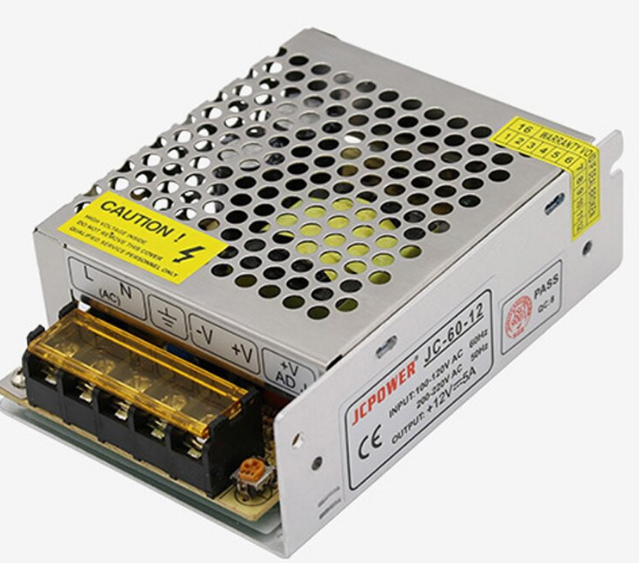
\includegraphics[width=6cm]{ch4/12V_Power_Supply.png} % replace with image path
    \caption{12V Power Supply}
    \label{fig:12v_power_supply}
\end{figure}

The main power supply comes from a 12V external power supply, which provides enough voltage for all the components and keeps the voltage from dropping and interfering with system performance. The Arduino microcontroller is powered via its VIN pin, so it can function without the need for a USB connection and maintains a stable 5V logic output for sensor and actuator control. The NEMA 17 stepper motors that operate the inspection tray and density sorter are directly powered from the 12V supply and fed into L298N motor drivers to adjust voltage and monitor current flow. Operating these motors at 12V provides best torque output, which is vital in ensuring consistent movement during the sorting process.

\begin{figure}[H]
    \centering
    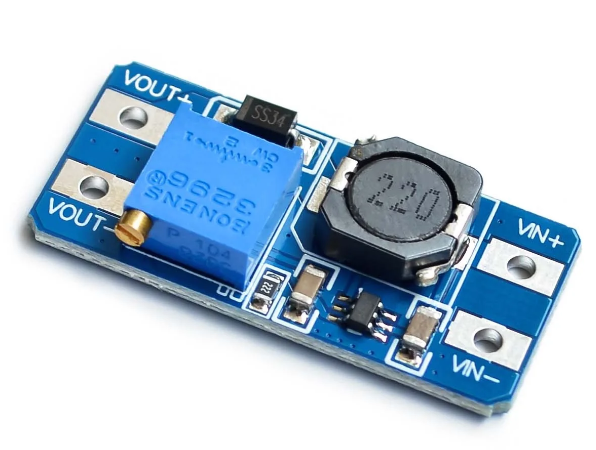
\includegraphics[width=6cm]{ch4/MT3608_Step-Up_Module.png} % replace with image path
    \caption{MT3608 Step-Up Module}
    \label{fig:mt3608}
\end{figure}

For the top feeder mechanism, a step-up module is needed to supply the sufficient voltage needed for the motor–6V. From the 5V output of the Arduino, the step-up module will be utilized to convert it into 6V.

\section{Computer Vision System}
% TODO: Write content
\subsection{Image Processing}

\begin{figure}[H]
    \centering
    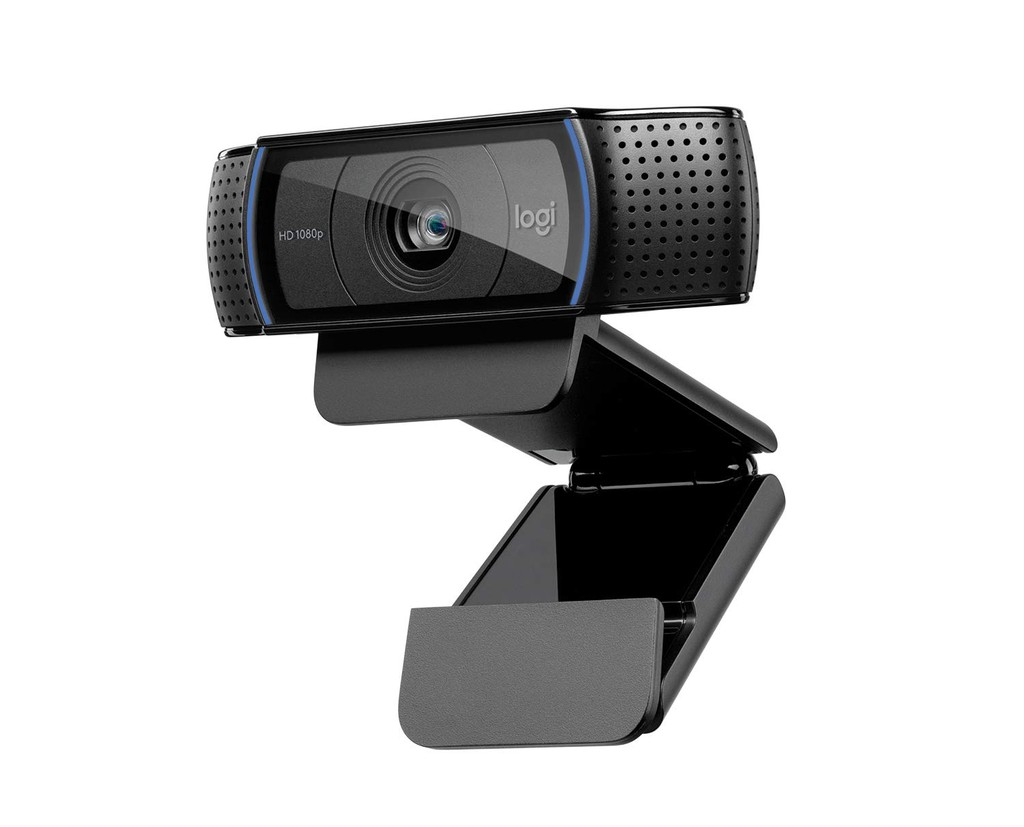
\includegraphics[width=6cm]{ch4/c920_cam.png} % replace with image path
    \caption{C920 Camera}
    \label{fig:c920_camera}
\end{figure}

The system requires clear images of the coffee beans for accurate processing by the detection and classification models. Two C920 cameras will be used to capture images from opposite sides of each bean—one positioned on top and the other at the bottom. The captured images will then be processed within the laptop using the detection and classification models to identify and categorize the beans.

\subsection{Object Detection and Classification Models}

The object detection model identifies and isolates the coffee beans from the background. For this task, different models were explored:

\begin{enumerate}
	\item \textbf{RF-DETR}
	 
	A transformer-based object detection model that eliminates the need for anchor boxes, improving small object detection.

	\item \textbf{YOLOv11}
	
	A CNN-based YOLO variant that incorporates the C3k2 block, SPPF, and C2PSA components to enhance feature extraction and detection accuracy.

	\item \textbf{YOLOv12}
	
	The latest YOLO version and attention-centric model that integrates transformer-based components to enhance performance while maintaining real-time efficiency.
\end{enumerate}

\subsection{Object Classification Models}
Following detection, each identified coffee bean was cropped and classified based on its defect type. The classification models used included:

\begin{enumerate}
	\item \textbf{EfficientNetV2}
	 
	A convolutional neural network (CNN) designed for high efficiency and accuracy, balancing computational cost and performance.
	
	\item \textbf{YOLOv8}
	
	A lightweight yet highly accurate model that supports both object detection and classification, making it suitable for real-time applications.

	\item \textbf{YOLOv11}
	
	A classification-specific adaptation of YOLOv11, leveraging enhanced feature extraction techniques for defect recognition.
	
	\item \textbf{YOLOv12}
	
	A classification variant of YOLOv12, incorporating advanced attention mechanisms to improve accuracy.
\end{enumerate}

\section{Serial Communication}

Serial communication is used for sensors and motors for arduino due to the simplicity, reliability and efficient transfer of data between different devices. The precision scale uses a RS232 and a MAX TTL converter to send the data from the precision to the arduino to get the weight values of each green coffee bean. To sort out the good from defective beans the system utilizes a servo motor. The data from python is received by the arduino through serial communication. The python side is responsible for the decision and defect classification while the arduino is responsible for controlling the servo motor.  

\section{Graphical User Interface (GUI)}

% TODO: Update design to consider new features (Tracking which defects are present, density details, the recommendation based on thresholding, the speed of system, runtime, accessibility etc.)
\begin{figure}[h]
    \centering
    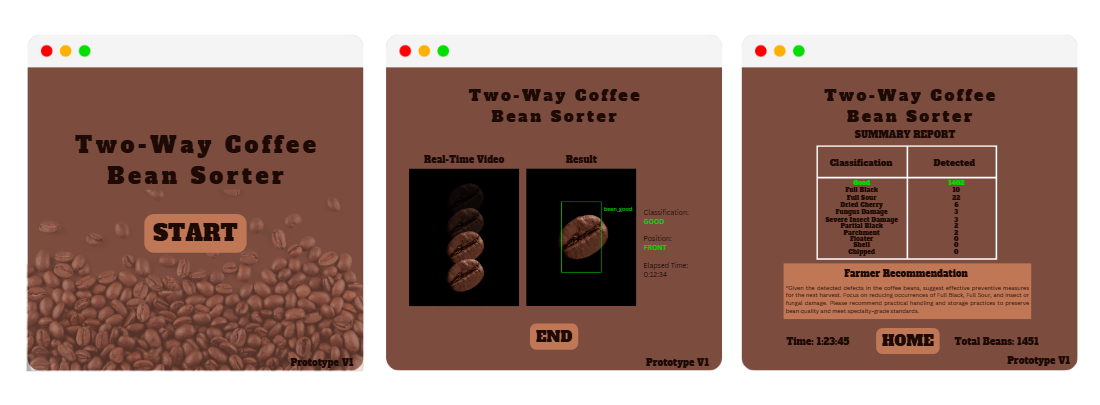
\includegraphics[width=12cm]{ch5/GUI.png} % replace with image path
    \caption{Graphical User Interface}
    \label{fig:gui}
\end{figure}

The proposed system would be integrating a graphical user interface developed using PyGui and ChatGPT API. The GUI would serve as the control center platform for the system. This would provide real-time feedback and insights for users. As shown in Figure 8, a concept of how the GUI would interact with the system would be a start button, once the button is executed the system would then be expecting inputs and start sorting. There would be real-time feedback during the sorting process, then some visual markers to indicate their classification, and an elapsed time so the user would be aware of the time of the sorting process. Once the system is done, the user can click the end button and the summary report would generate in an orderly manner, providing tables of classification that was detected through the process. In the bottom part of the GUI, ChatGPT API would be integrated and would offer recommendations based on the detected quality and classification of the coffee beans. 

\section{Density Analysis}
The density analysis works by using a precision scale to measure the mass of the bean. To get the data from the precision scale, serial communication is used from the scale to an arduino nano. This is done by using a RS232 with a Max TTL converter for the arduino to read the data from the precision scale. To sort out the good from defective beans the system utilizes a servo motor for the density sorting mechanism. The servo motor is used to sort the dense from the less dense beans. The sorting mechanism developed consists of gears and cross-shaped modules to properly capture the beans and properly sort them out. 

\section{Technical Standards}

\subsection{Hardware}
In the design and development of the system, the group incorporated and followed a series of technical standards. One of which is ISO 12100:2010 – Safety of Machinery, where general principles for risk assessment and reduction are discussed. Thus, the system is designed, while keeping in mind the hazards associated with moving parts, making sure that all moving parts in the system do not need to be touched for operations. An emergency stop is also integrated into the system to stop all the moving parts in case of undesirable incidents \cite{International_Organization_for_Standardization_2010}. 

On top of this, ISO 14121-1 – Risk Assessment for Machinery was also followed to further assess the potential risks throughout the system. The standard includes identifying and quantifying hazards such as electrical short circuits, faulty wirings, and motor overheating \cite{International_Organization_for_Standardization_2007}. With this, the system included protective enclosures for the electrical wirings, proper grounding of the circuits, and controlled motor actuation. More specifically, for motors, it was made sure that the design has sufficient voltage and ampere to power the different kinds of motors used with the use of L298N, and MT3608 modules. These are the main components for adjusting motor speeds dynamically during the sorting process.

Lastly, ISO 30071-1 was standard used to provide sufficient lighting during data collection, and real time bean inspection during sorting process. This standard helps ensure consistent and non-glare lighting conditions, which are essential for the machine vision cameras to accurately capture bean features \cite{International_Organization_for_Standardization_2019}. Uniform illumination improves the reliability of image classification by reducing shadow artifacts and reflections, thereby enhancing overall detection performance.

\subsection{Software}

For the software side of the system, the first applicable standard is ISO/IEC 25024 – Systems and Software Engineering – Measurement of Data Quality, which offers a systematic method for measuring the quality of datasets utilized in information systems \cite{International_Organization_for_Standardization_2015}. This standard was used during the dataset gathering and training for the different coffee bean defects like black, sour, insect damage, fungus damage, broken, floaters, and dried cherry. Practically, this included pre-processing the image data to eliminate noise, balance class distribution, and verify ground truth labels. 

Lastly, ISO/IEC 23053 – Framework for Artificial Intelligence (AI) offers a reference architecture to build and integrate machine learning building blocks \cite{International_Organization_for_Standardization_2022}. This standard was highly applicable in determining the design of the machine vision module, where a pre-trained deep learning model is utilized for the classification of bean defects. This standard provides guidelines on best practice for the overall machine learning cycle, ranging from data acquisition, feature extraction, and model training through to model evaluation, deployment, and monitoring. 

\subsection{Green Coffee Bean Sorting}

For sorting green coffee beans, Specialty Coffee Association of America (SCAA) Standards for Green Coffee Bean Sorting was incorporated to maintain conformity. The standards set the definition for the classification of primary and secondary defects (i.e., black, sour, insect-damaged, broken, and floater beans) and sets the maximum allowable defect counts for specialty-grade coffee. The SCAA standards were applied to mark the training set of the machine vision model and also to set up the thresholds of defect classification, so visually defective beans can be correctly classified and rejected. Also, the sorting mechanism based on density points towards SCAA bean weight and volume guidelines using a precision scale and ToF sensor to sort beans based on within-acceptability density limits.

On the other hand, the system also adheres to PNS/BAFS 341:2022, the Philippine National Standard for Agricultural Machinery – Coffee Green Bean Grader – Specifications and Methods of Test \cite{Bureau_of_Agriculture_and_Fisheries_Standards_2022}. It sets local criteria for testing coffee grading equipment on performance, safety, construction aspects, and methods of test. For the purposes of this research, PNS/BAFS 341:2022 is used as a reference for the design of the sorting mechanism, specifically in terms of the materials used in construction, handling of beans, and the efficiency with which the mechanical and electronic subsystems segregate. It also guides the testing procedure employed to verify sorting precision, capacity, and rates of misclassification under test conditions. 

	%\stopcontents[chapters]
	\cleardoublepage
	
	%%%%%%%%%%%%%%%%%%%%%%%%%%%%%%%%%%%%%%%%%%%%%%%%
	\chapter{Methodology} 
	\label{ch:method} 
	%\startcontents[chapters]
	%\begin{SingleSpace}	
	%	\Mprintcontents 
	%\end{SingleSpace}
	\begin{center}
	{\scriptsize
		\begin{tabularx}{\textwidth}{p{0.2\textwidth}|p{0.6\textwidth}|p{0.1\textwidth}}
			\caption{Summary of methods for reaching the objectives} \label{tab:methods_per_objective} \\
			\hline 
			\hline 
			\textbf{Objectives} & 
			\textbf{Methods} &
			\textbf{Locations}\\ 
			\hline 
			\endfirsthead
			\multicolumn{3}{c}%
			{\textit{Continued from previous page}} \\
			\hline
			\hline 
			\textbf{Objectives} & 
			\textbf{Methods} &
			\textbf{Locations}\\ 
			\hline 
			\endhead
			\hline 
			\multicolumn{3}{r}{\textit{Continued on next page}} \\ 
			\endfoot
			\hline 
			\endlastfoot
			\hline
			
			
			\Paste{GO} & 

			\begin{itemize}
				\item DDR Methodology
				\item Description of the System
			\end{itemize}
			
			& Sec.~\ref{sec:description_system} on p.~\pageref{sec:description_system} 

			Sec.~\ref{sec:research_design} on p.~\pageref{sec:research_design}
			\\ \hline
			
			\Paste{SO1} & 
			\begin{itemize}
				\item Dataset Collection
				\item Manual Sorting
			\end{itemize} & 
			
			Sec.~\ref{sec:dataset_collection} on p.~\pageref{sec:dataset_collection} \\ \hline
			
			
			\Paste{SO2} & 

			\begin{itemize}
				\item Data Collection
				\item Dataset preprocessing
				\item Model Training
				\item Serial Communication
			\end{itemize} 
	
			& Sec.~\ref{sec:dataset_collection} on p.~\pageref{sec:dataset_collection}
			
			Sec.~\ref{sec:dataset_prep_and_model_training} on p.~\pageref{sec:dataset_prep_and_model_training}\\ \hline

			Sec.~\ref{sec:serial_communication} on p.~\pageref{sec:serial_communication}
			
			\Paste{SO3} & 
			\begin{itemize}
				\item Dataset preprocessing
				\item Model Training
			\end{itemize} 
			& Sec.~\ref{sec:dataset_prep_and_model_training} on p.~\pageref{sec:dataset_prep_and_model_training}\\ \hline
			
			
			\Paste{SO4} &
			\begin{itemize}
				\item Density Threshold Calibration Using Water Displacement Method
				\item Density Sorter
			\end{itemize}
			& Sec.~\ref{sec:density_threshold_calibration} on p.~\pageref{sec:density_threshold_calibration}
			
			Sec.~\ref{sec:density_sorter} on p.~\pageref{sec:density_sorter} \\ \hline
						
		\end{tabularx}
	}
\end{center}

\section{Description of the System}
\label{sec:description_system}

\begin{figure}[H]
    \centering
    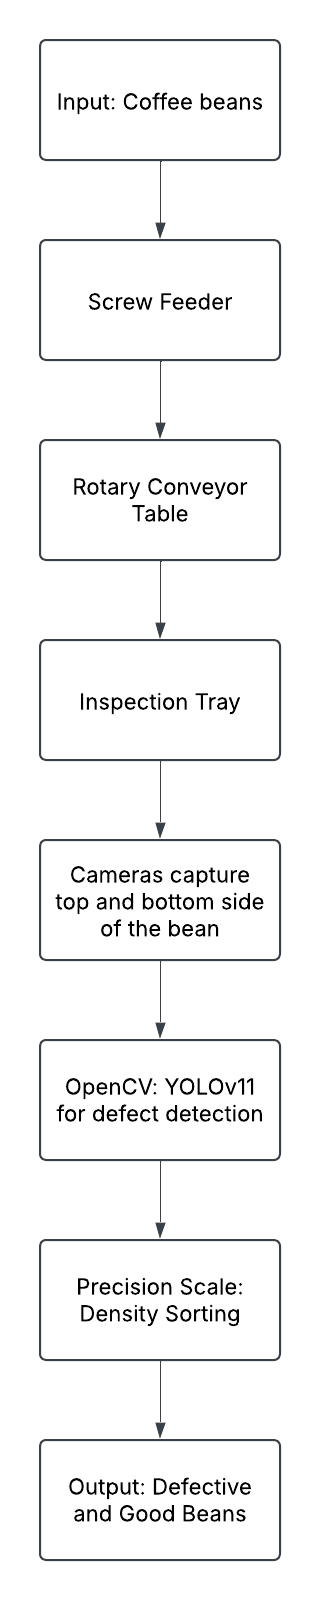
\includegraphics[width=14cm]{ch5/system_block_diagram.png}
    \caption{System Block Diagram}
    \label{fig:system_block_diagram}
\end{figure}

The system is an automated green coffee bean sorting machine, utilizing machine vision. Firstly, the coffee beans are introduced into the system through a funnel, which directs them to a conveyor belt mechanism. The green coffee beans are sorted depending on their visual characteristics. In this process, the physical qualities of the bean are analyzed such as size, color, and defect. If the bean is defective, the system will automatically sort it out. Then, all the non-defective beans will go through the second stage of the system. In the second stage, there will be a precision scale. With the volume and mass of the bean in hand, the density of the bean can be estimated. Depending on the density threshold set by the user, the bean will be classified whether it is good or not.

\begin{figure}[H]
    \centering
    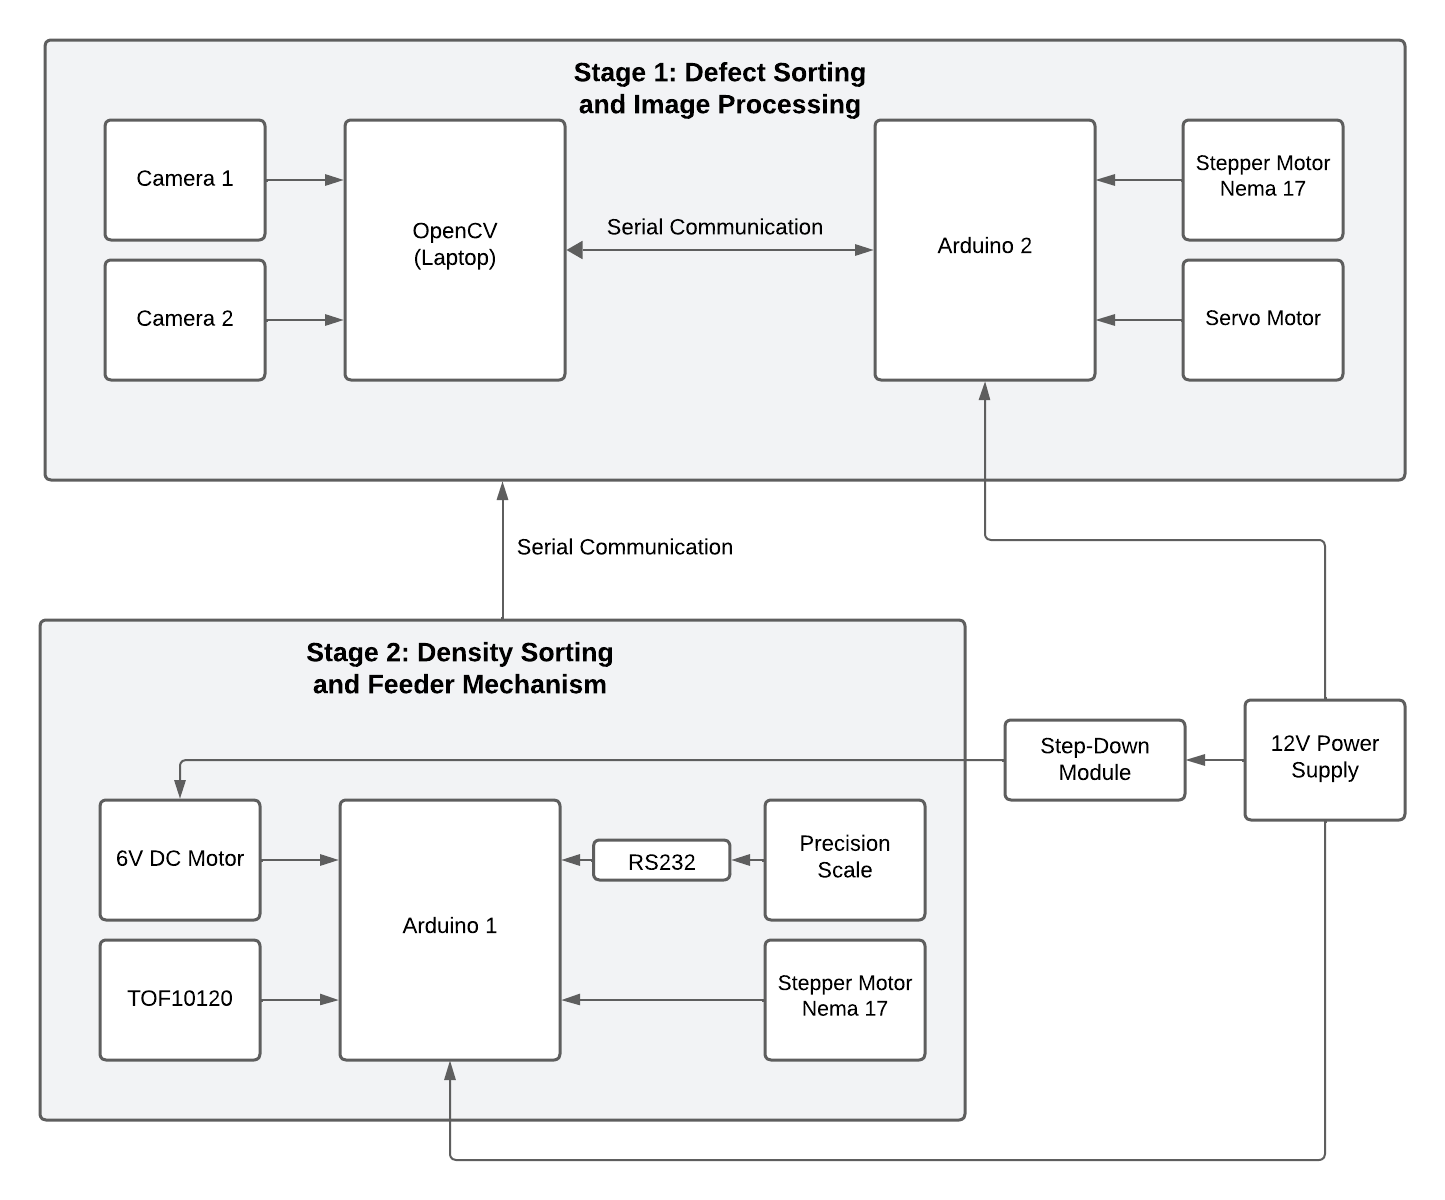
\includegraphics[width=14cm]{ch5/Schematic_Diagram_of_the_System.png}
    \caption{Schematic Diagram of the System}
    \label{fig:system_schematic_diagram}
\end{figure}

Figure \ref{fig:system_schematic_diagram} shows the schematic diagram of the proposed system. Arduino Uno microcontroller makes all the mechanical components such as the servo motor, stepper motors, and the conveyor belt. The servo motor controls the  rotating mechanism for bean sorting. On the other hand, the stepper motors operate a slide mechanism to direct the beans. Two cameras, integrated with OpenCV via Python, handle machine vision algorithms, and image processing for defect detection of the beans. A ToF10120 sensor provides precise distance measurement. A precision weighing scale measures the density of each bean for classification. The Arduino communicates with the OpenCV system through serial communication, ensuring smooth coordination.

\begin{figure}[H]
    \centering
    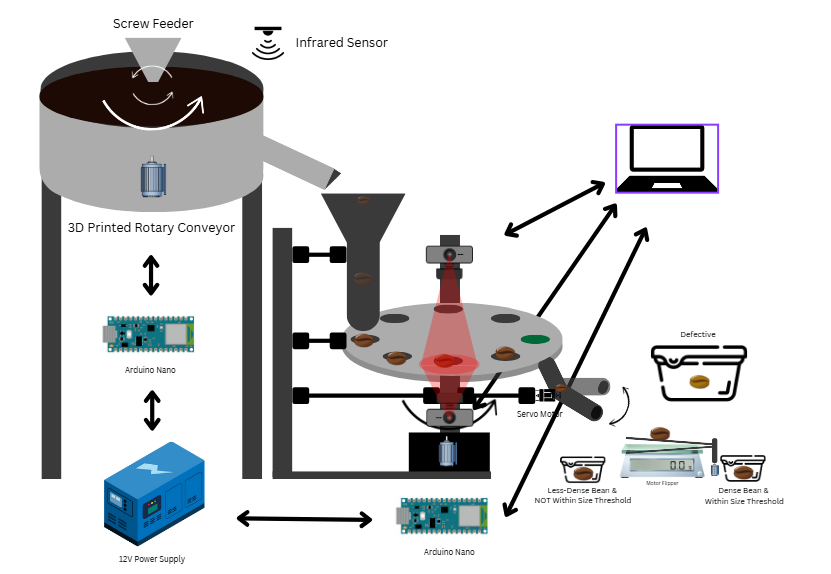
\includegraphics[width=14cm]{ch5/Overview_Of_The_System.png}
    \caption{Design Overview of the System}
    \label{fig:system_design_overview}
\end{figure}

Figure \ref{fig:system_design_overview} shows the design overview of the system. Beans are first arranged through a hopper and a conveyor belt. On top of the conveyor belt, a 3D-printed guide is attached for the beans to maintain a linear formation. Then, the beans are expected to fall into another funnel attached to a tube. The tube is directly attached to a rotating mechanism that allows the beans to be inspected and sorted one-by-one. In this stage, defective beans are sorted out. Then, the non-defective beans are transferred onto the precision scale to analyze the density. The less-dense beans are sorted out of the batch.

\section{Research Design}
\label{sec:research_design}

\begin{figure}[H]
    \centering
    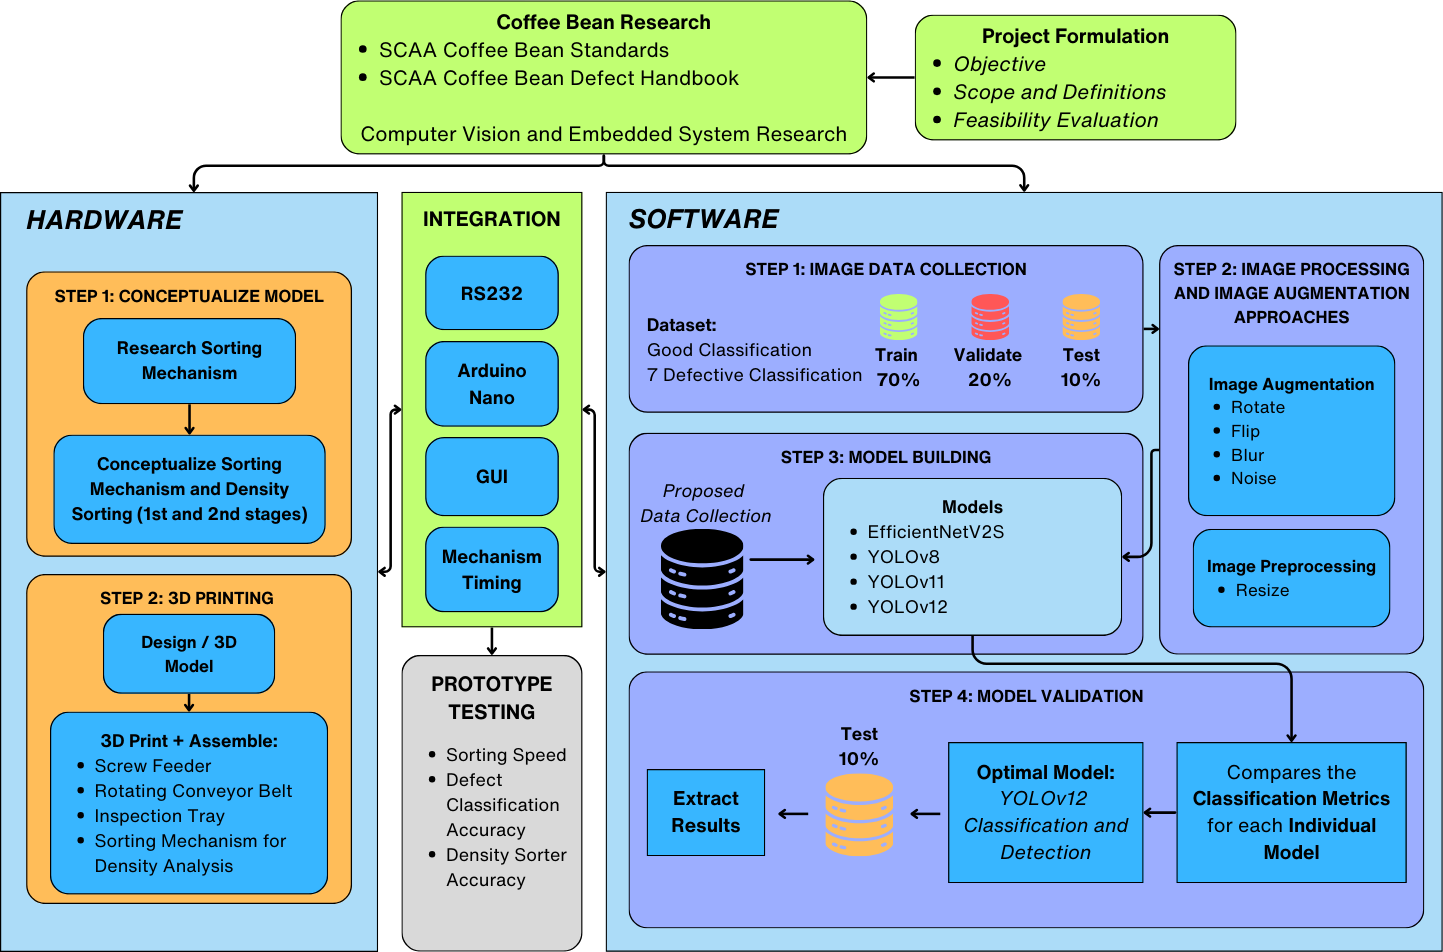
\includegraphics[width=\textwidth]{ch5/DDR_Research_Diagram_v2.png}
    \caption{Design and Development Research (DDR) Methodology}
    \label{fig:ddr_methodology}
\end{figure}

The researchers opted for a Design and Development Research model for the research. As shown in Figure \ref{fig:ddr_methodology},  there are multiple levels that were needed in order to develop a working prototype for the system. 



\section{Dataset Collection}
\label{sec:dataset_collection}

\begin{figure}[H]
    \centering
    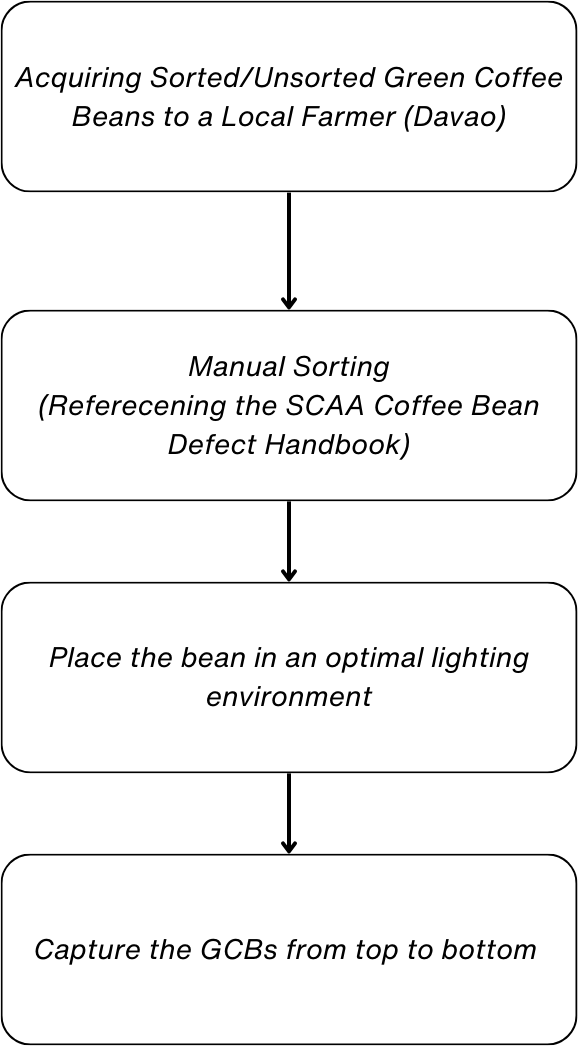
\includegraphics[width=6cm]{ch5/Datacollection_Process.png}
    \caption{Data Collection Process}
    \label{fig:data_collection_process}
\end{figure}
For dataset collection, Arabica green beans from a farm will be used. Each bean will be captured by a high-resolution camera under sufficient and consistent lighting. Proper lighting is crucial, as it directly affects the visibility of the bean’s physical features, minimizing shadows, grain, and other noise that could result from inconsistent illumination. The top and bottom side pictures of the beans are to be collected. In addition, defective beans of the same type and origin will be gathered to identify the different classification of defects (primary and secondary). This study focuses on defects such as Broken, Dried Cherry, Floater, Full Black, Full Sour, Fungus Damage, and Insect Damage. The dataset will include at least 500 images of good beans and a minimum of 200 images for each defect category. To expand the dataset and enhance model training, augmentation techniques such as scaling, rotation, and mirroring will be applied. 

\subsection{Dataset Collection and Model Training}

\begin{figure}[H]
    \centering
    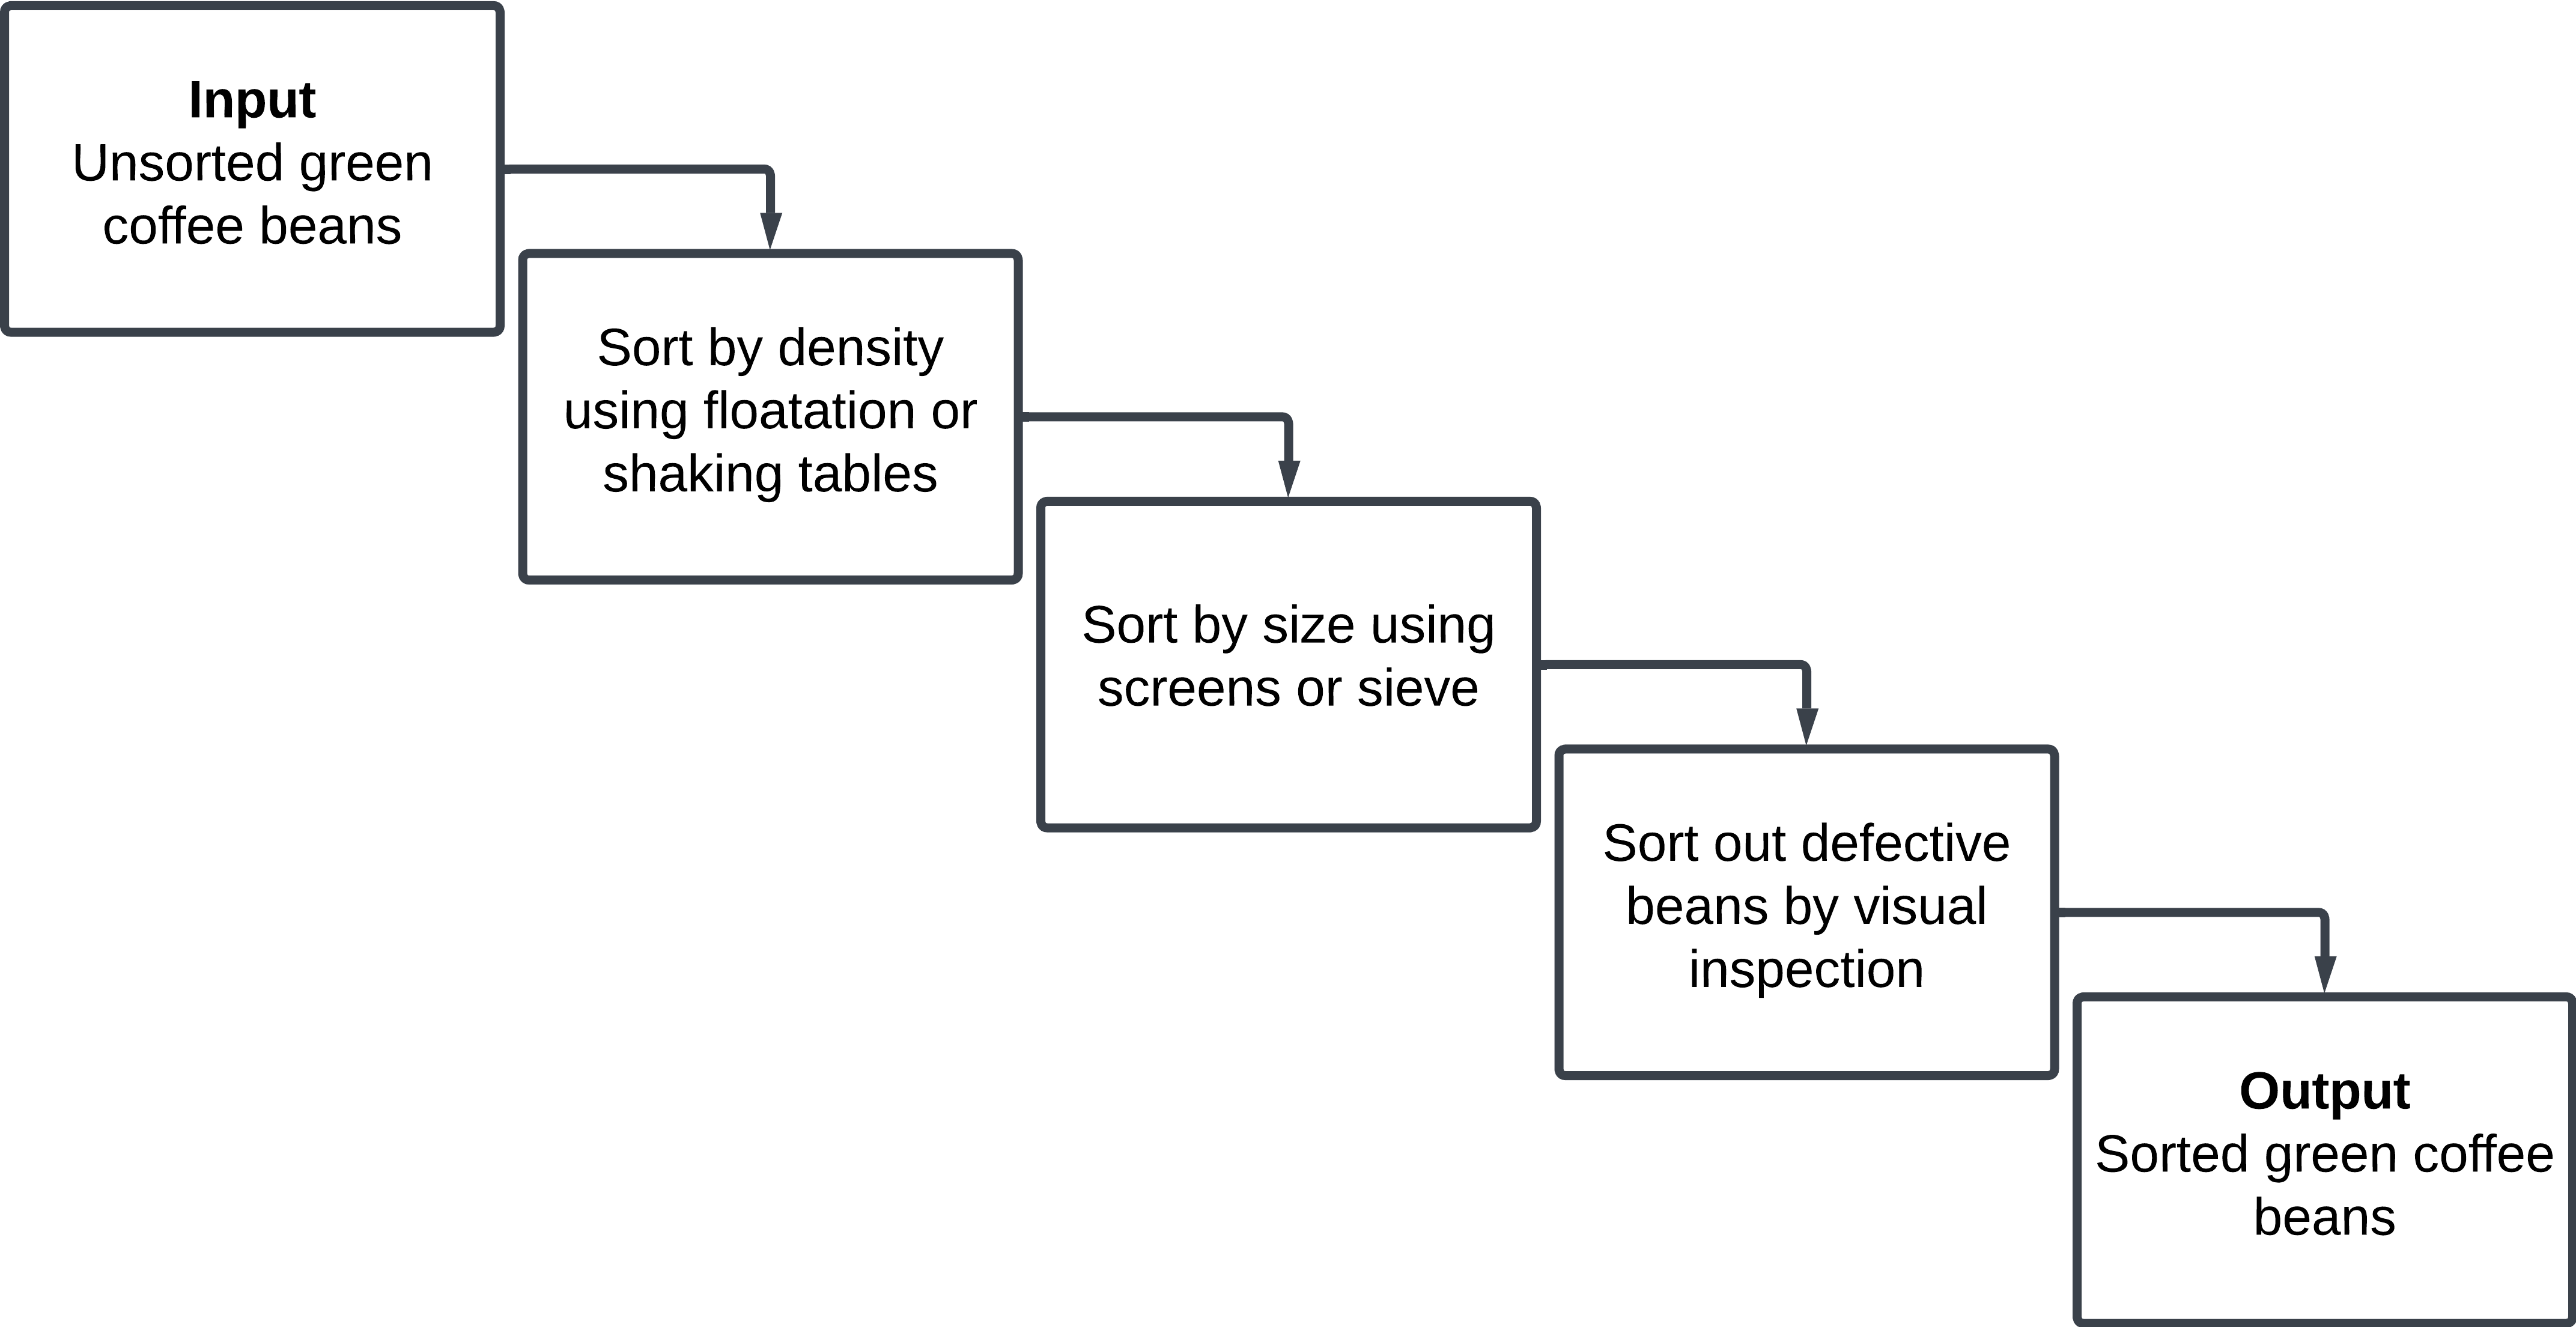
\includegraphics[width=12cm]{ch5/Manual_Sorting_Process.png}
    \caption{Manual Sorting Process}
    \label{fig:manual_sorting}
\end{figure}

% TODO: Fix citations for SCAA
The diagram in Figure \ref{fig:manual_sorting} depicts the representation of the process of manual sorting of unsorted green coffee beans through a series of steps. First, the beans are sorted by density using methods such as floatation or shaking tables. This helps in separating the denser beans, usually pertaining to a more developed and higher quality bean. Then, the beans are sorted by size using screens and sieves with specific dimensions depending on the variety of the beans. After this, a thorough visual inspection is performed by the sorters to identify and remove the defective beans from the batch. To ensure consistency and accuracy, the group follows the Specialty Coffee Association of America (SCAA) Standards Defect Handbook, which provide documentation and guidelines for identifying and classifying defective beans. Finally, the process results in the output of sorted green coffee beans, ready for further processing or sale. 
To ensure the dataset reflects real-world conditions, the group acquired Arabica green coffee beans from Davao. These beans were manually sorted to properly classify defective characteristics before capturing images for dataset creation. This step was crucial for improving the efficiency of batch image capture and ensuring accurate model training, making the system more applicable to Philippine coffee producers.

\subsection{Utilization of Open-Source Database}
% ! CHANGE `the group` statement, citation after Kaggle
To establish a foundation for the system's model, the group initially referenced an open-source dataset from Kaggle. This dataset provides an original 500x500px images of Arabica green coffee beans categorize as defective or good. This dataset also provided insights into how individual beans were captured, including factors such as lighting, camera positioning, focus, and resolution. By analyzing the dataset, the group gained a better understanding of how to achieve a high-quality data collection, ensuring that the collected dataset would contribute to high model accuracy when it is fed into the system.


\subsection{First Iteration of Dataset Collection}
\begin{figure}[H]
    \centering
    \includegraphics[width=10cm]{data_collection_setup.png}
    \caption{First Iteration of Data Collection Setup}
    \label{fig:data_collection_setup}
\end{figure}

\begin{figure}[H]
	\centering
	\begin{tabular}{cc}
		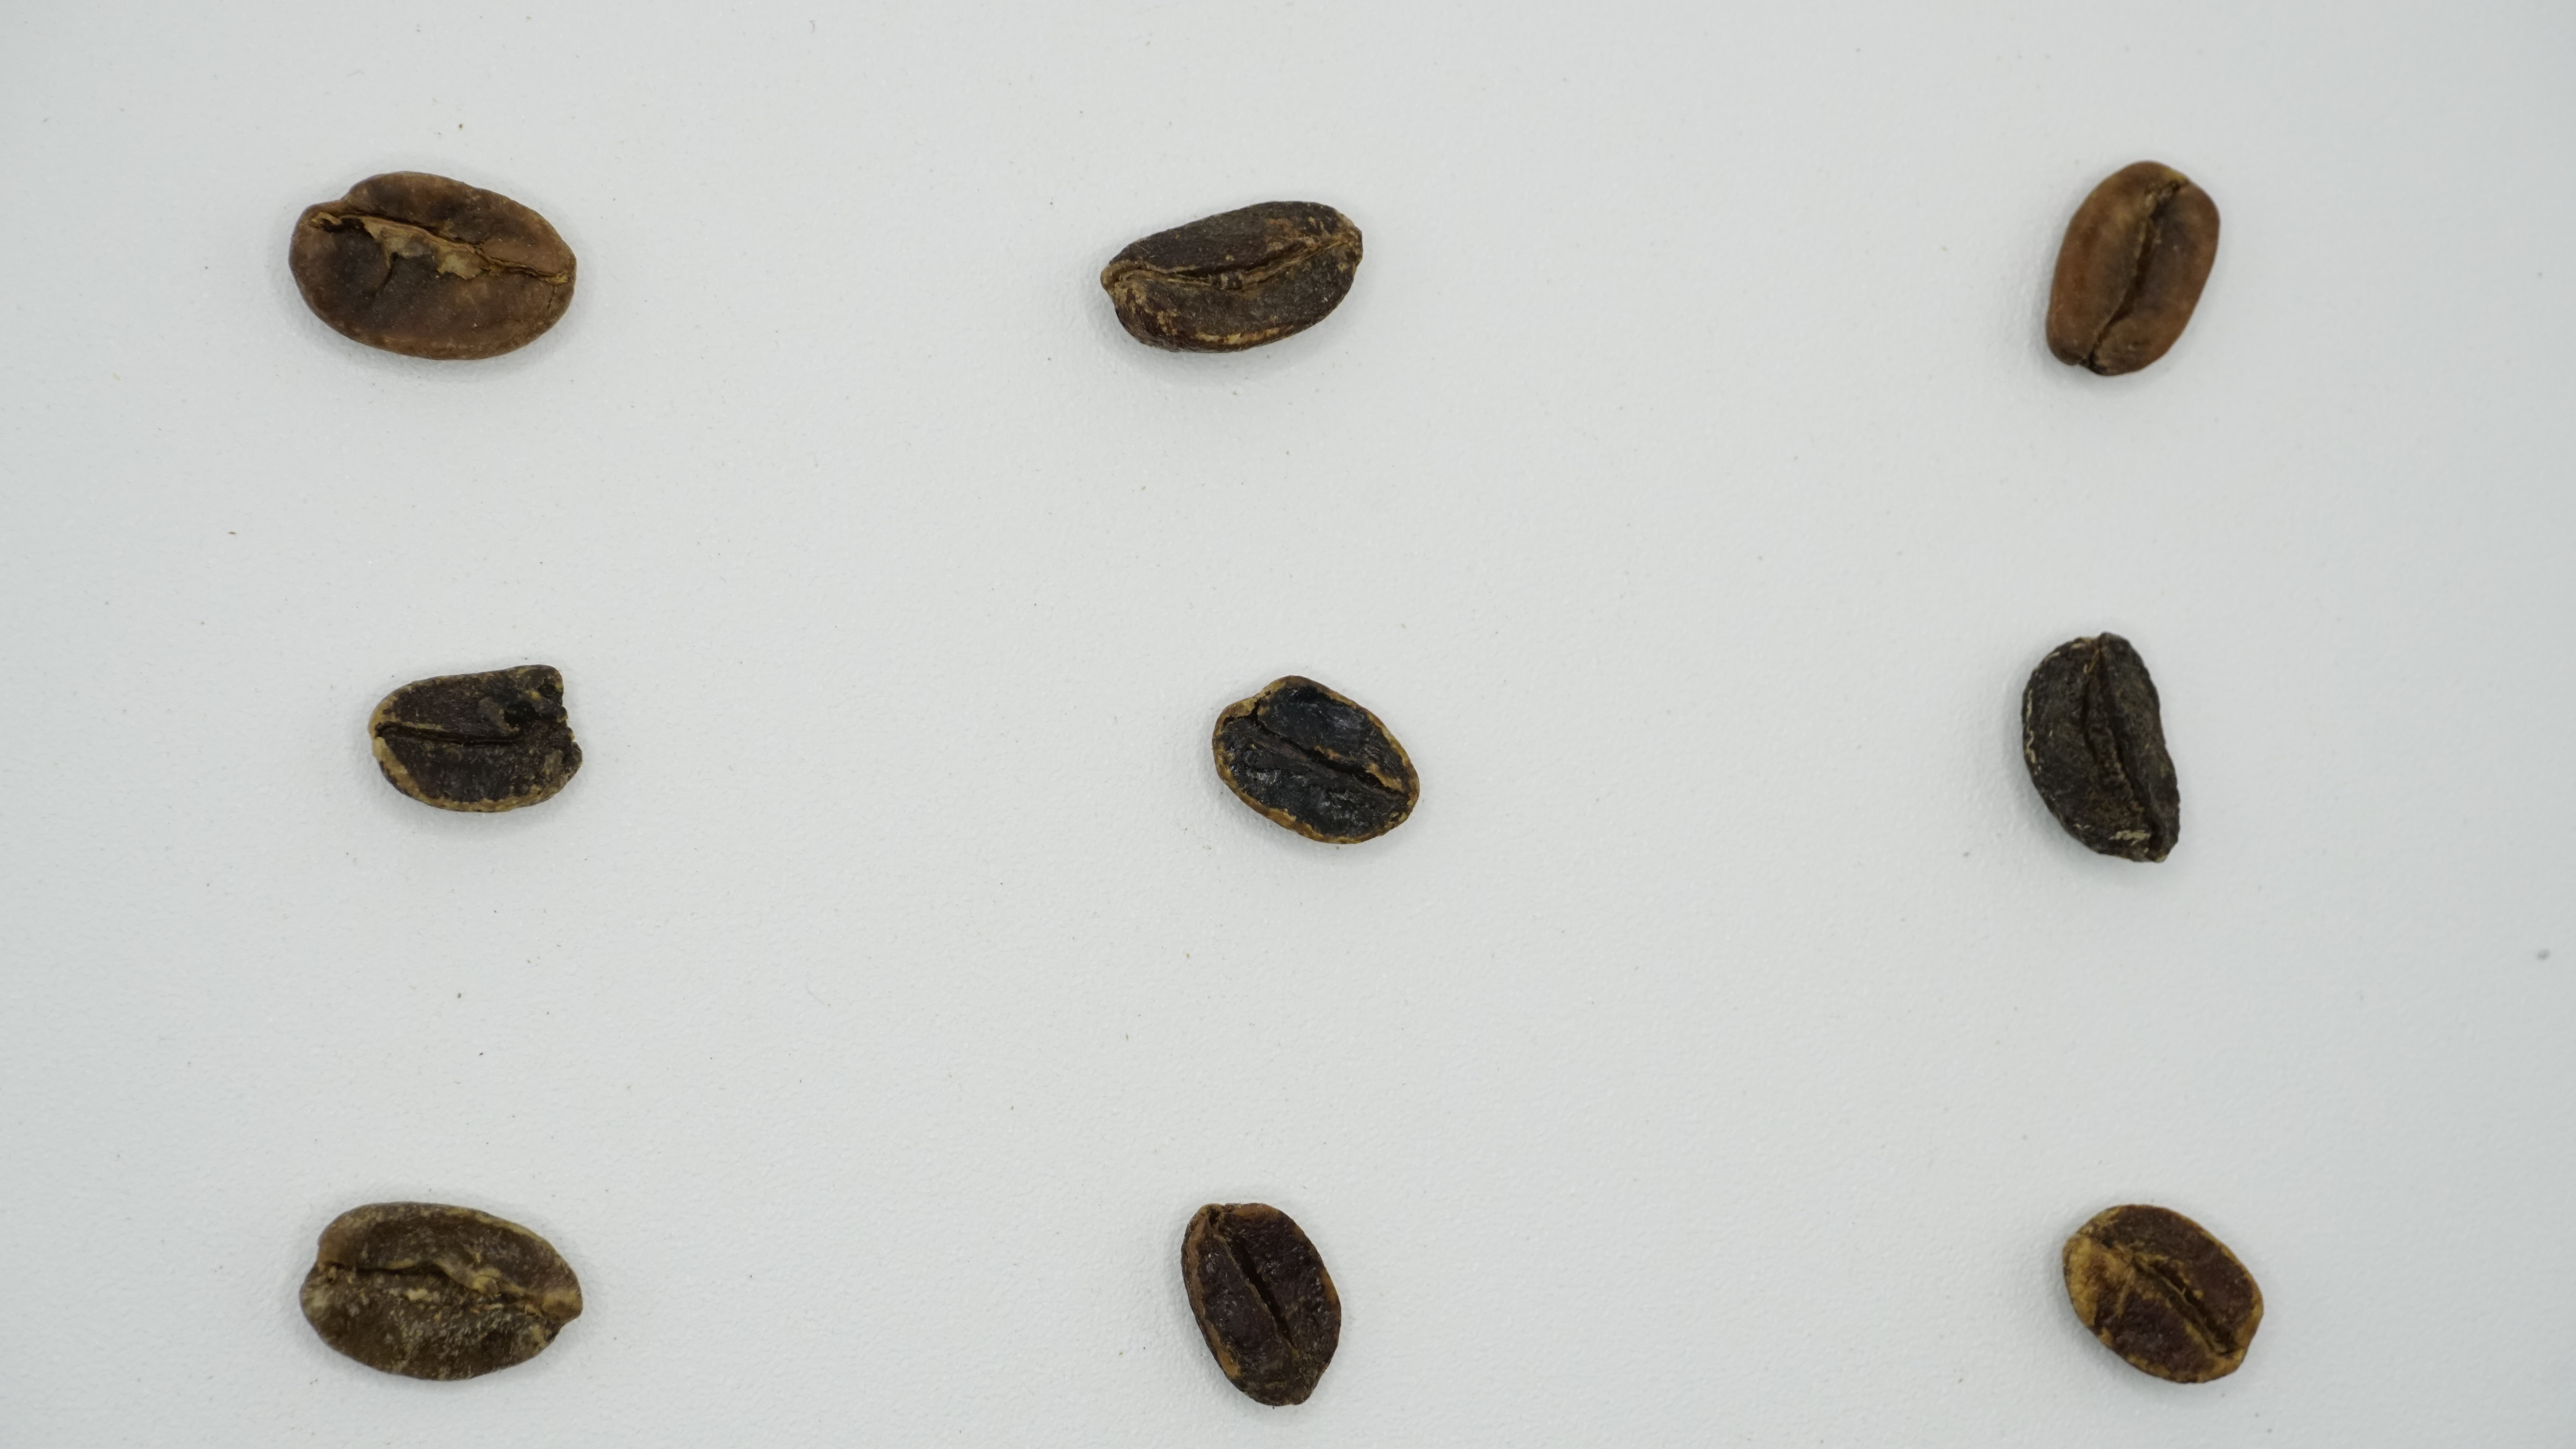
\includegraphics[width=0.3\textwidth]{ch5/1st-Iteration-Table/Black.JPG} &
		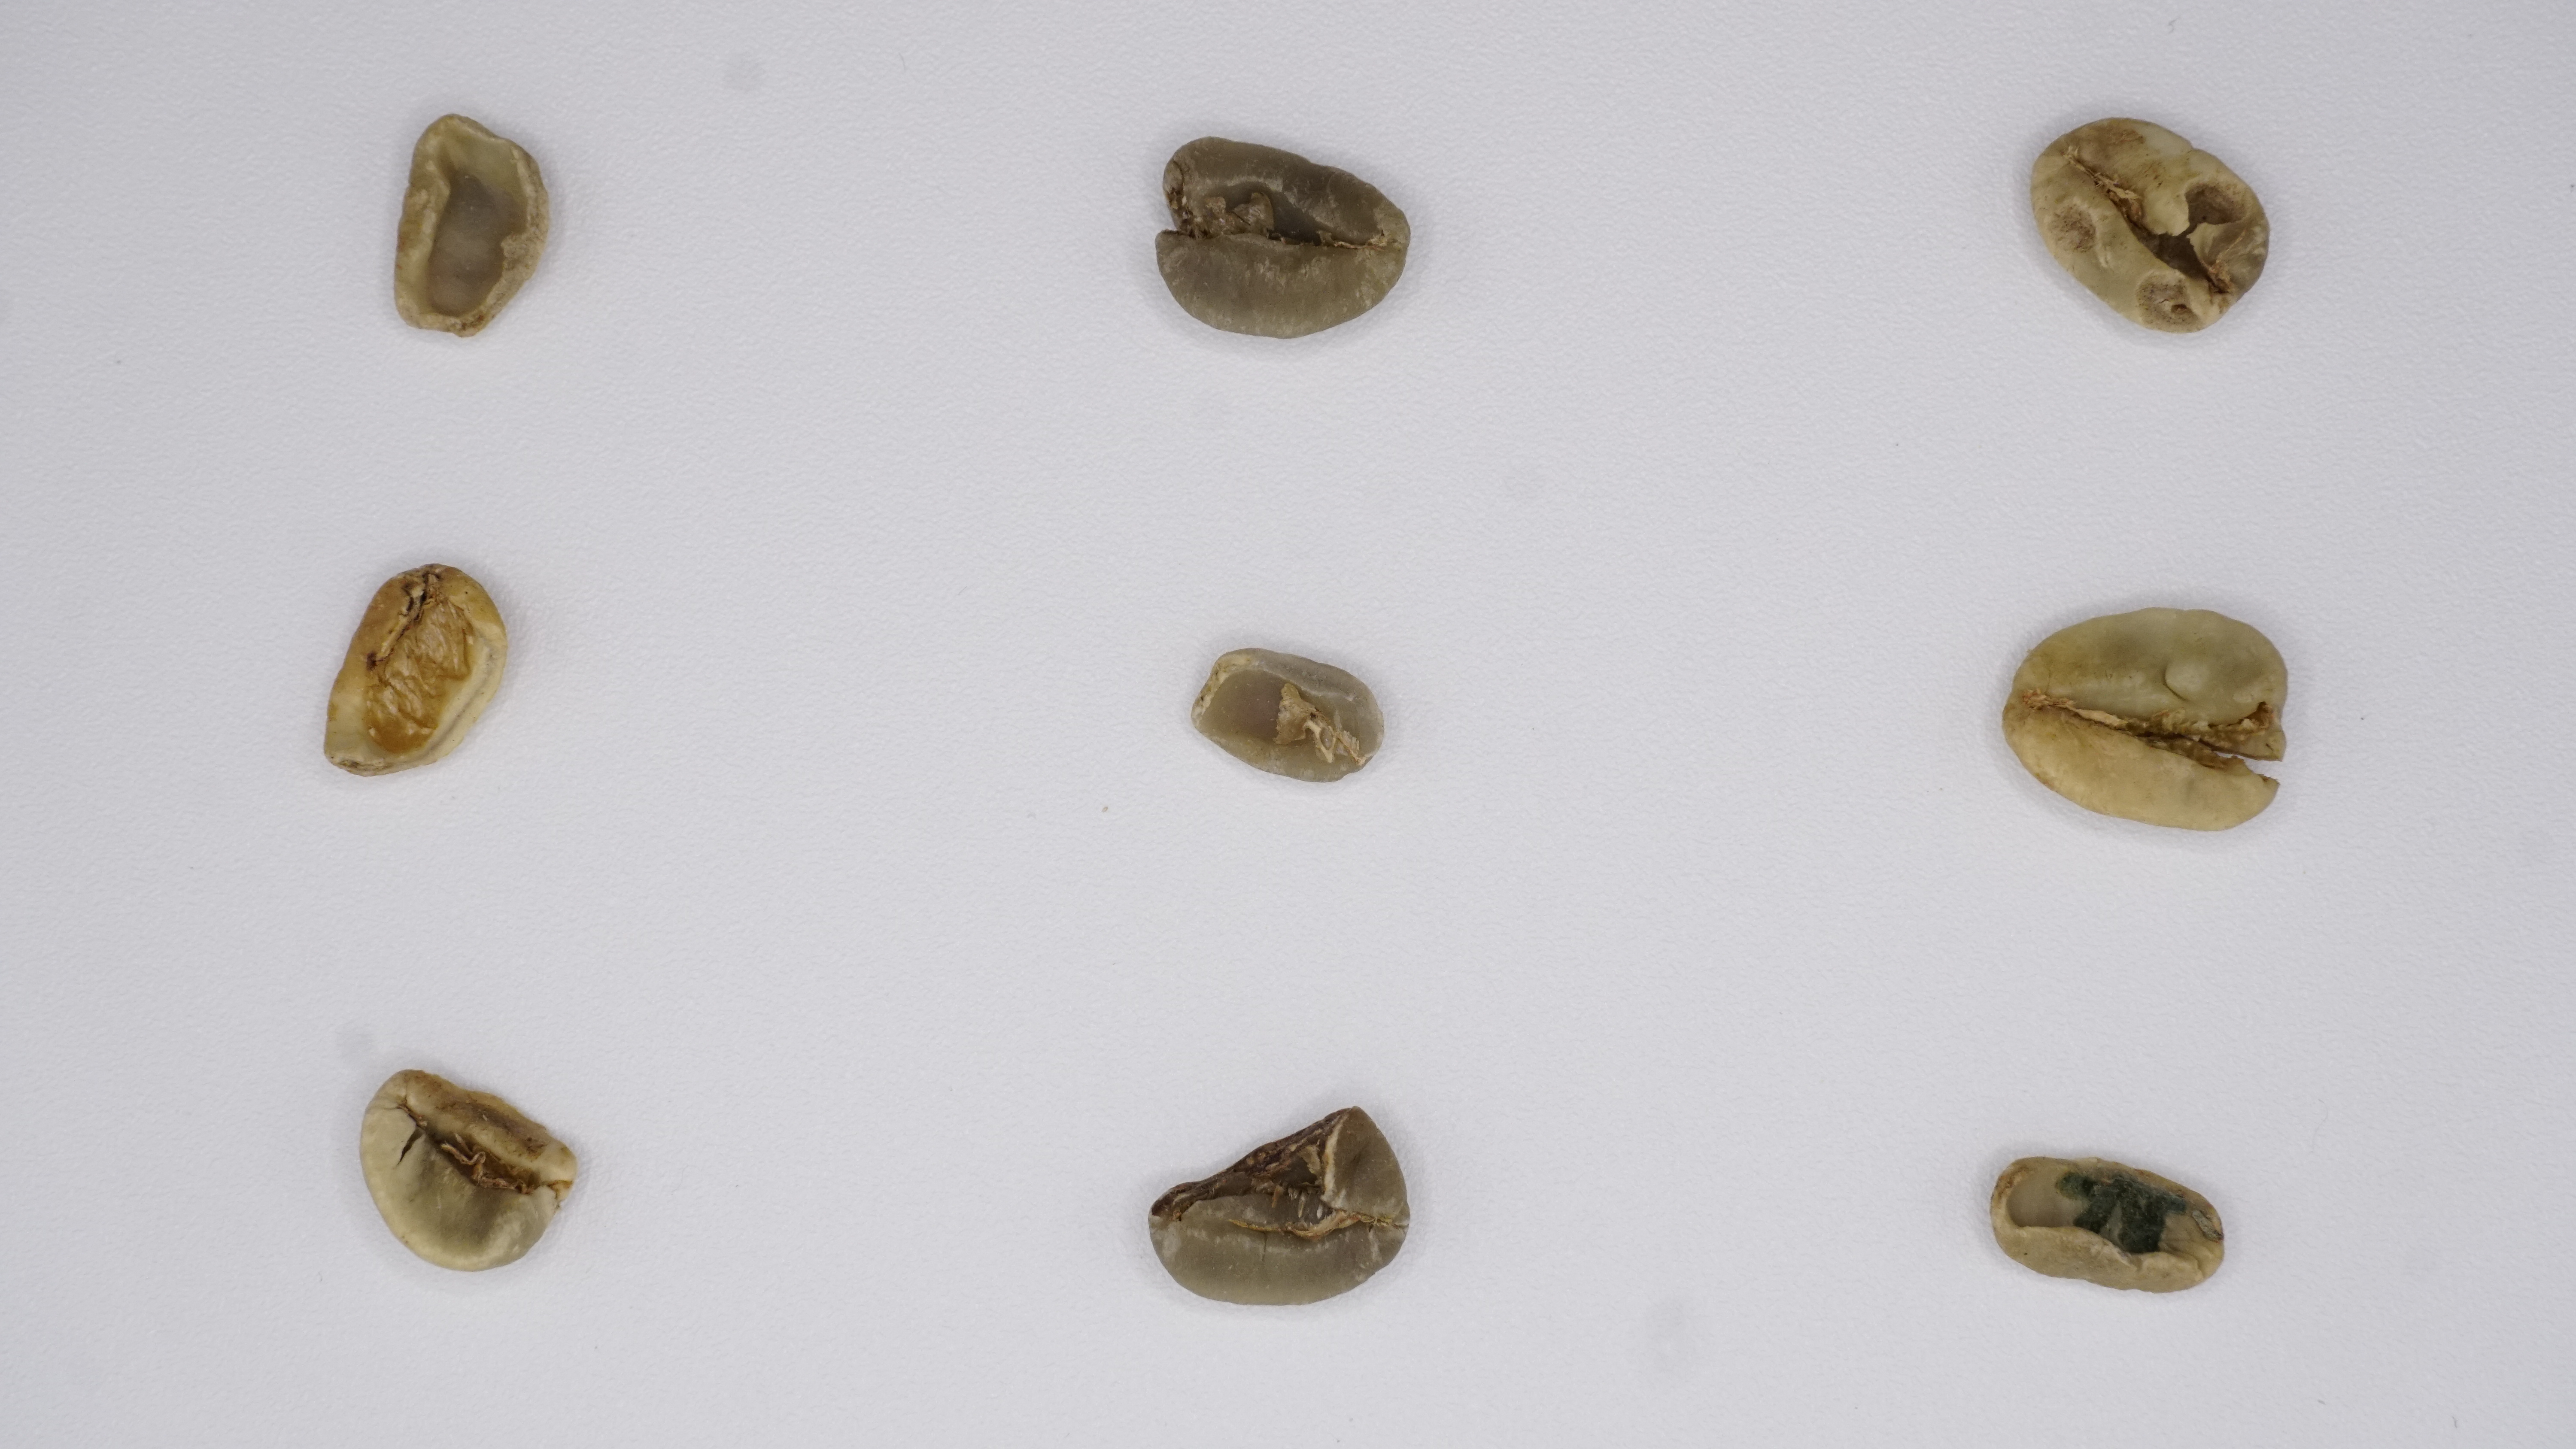
\includegraphics[width=0.3\textwidth]{ch5/1st-Iteration-Table/Broken.JPG} \\
		\textbf{Black}  & \textbf{Broken} \\[6pt]
	\end{tabular}
	\begin{tabular}{cc}
		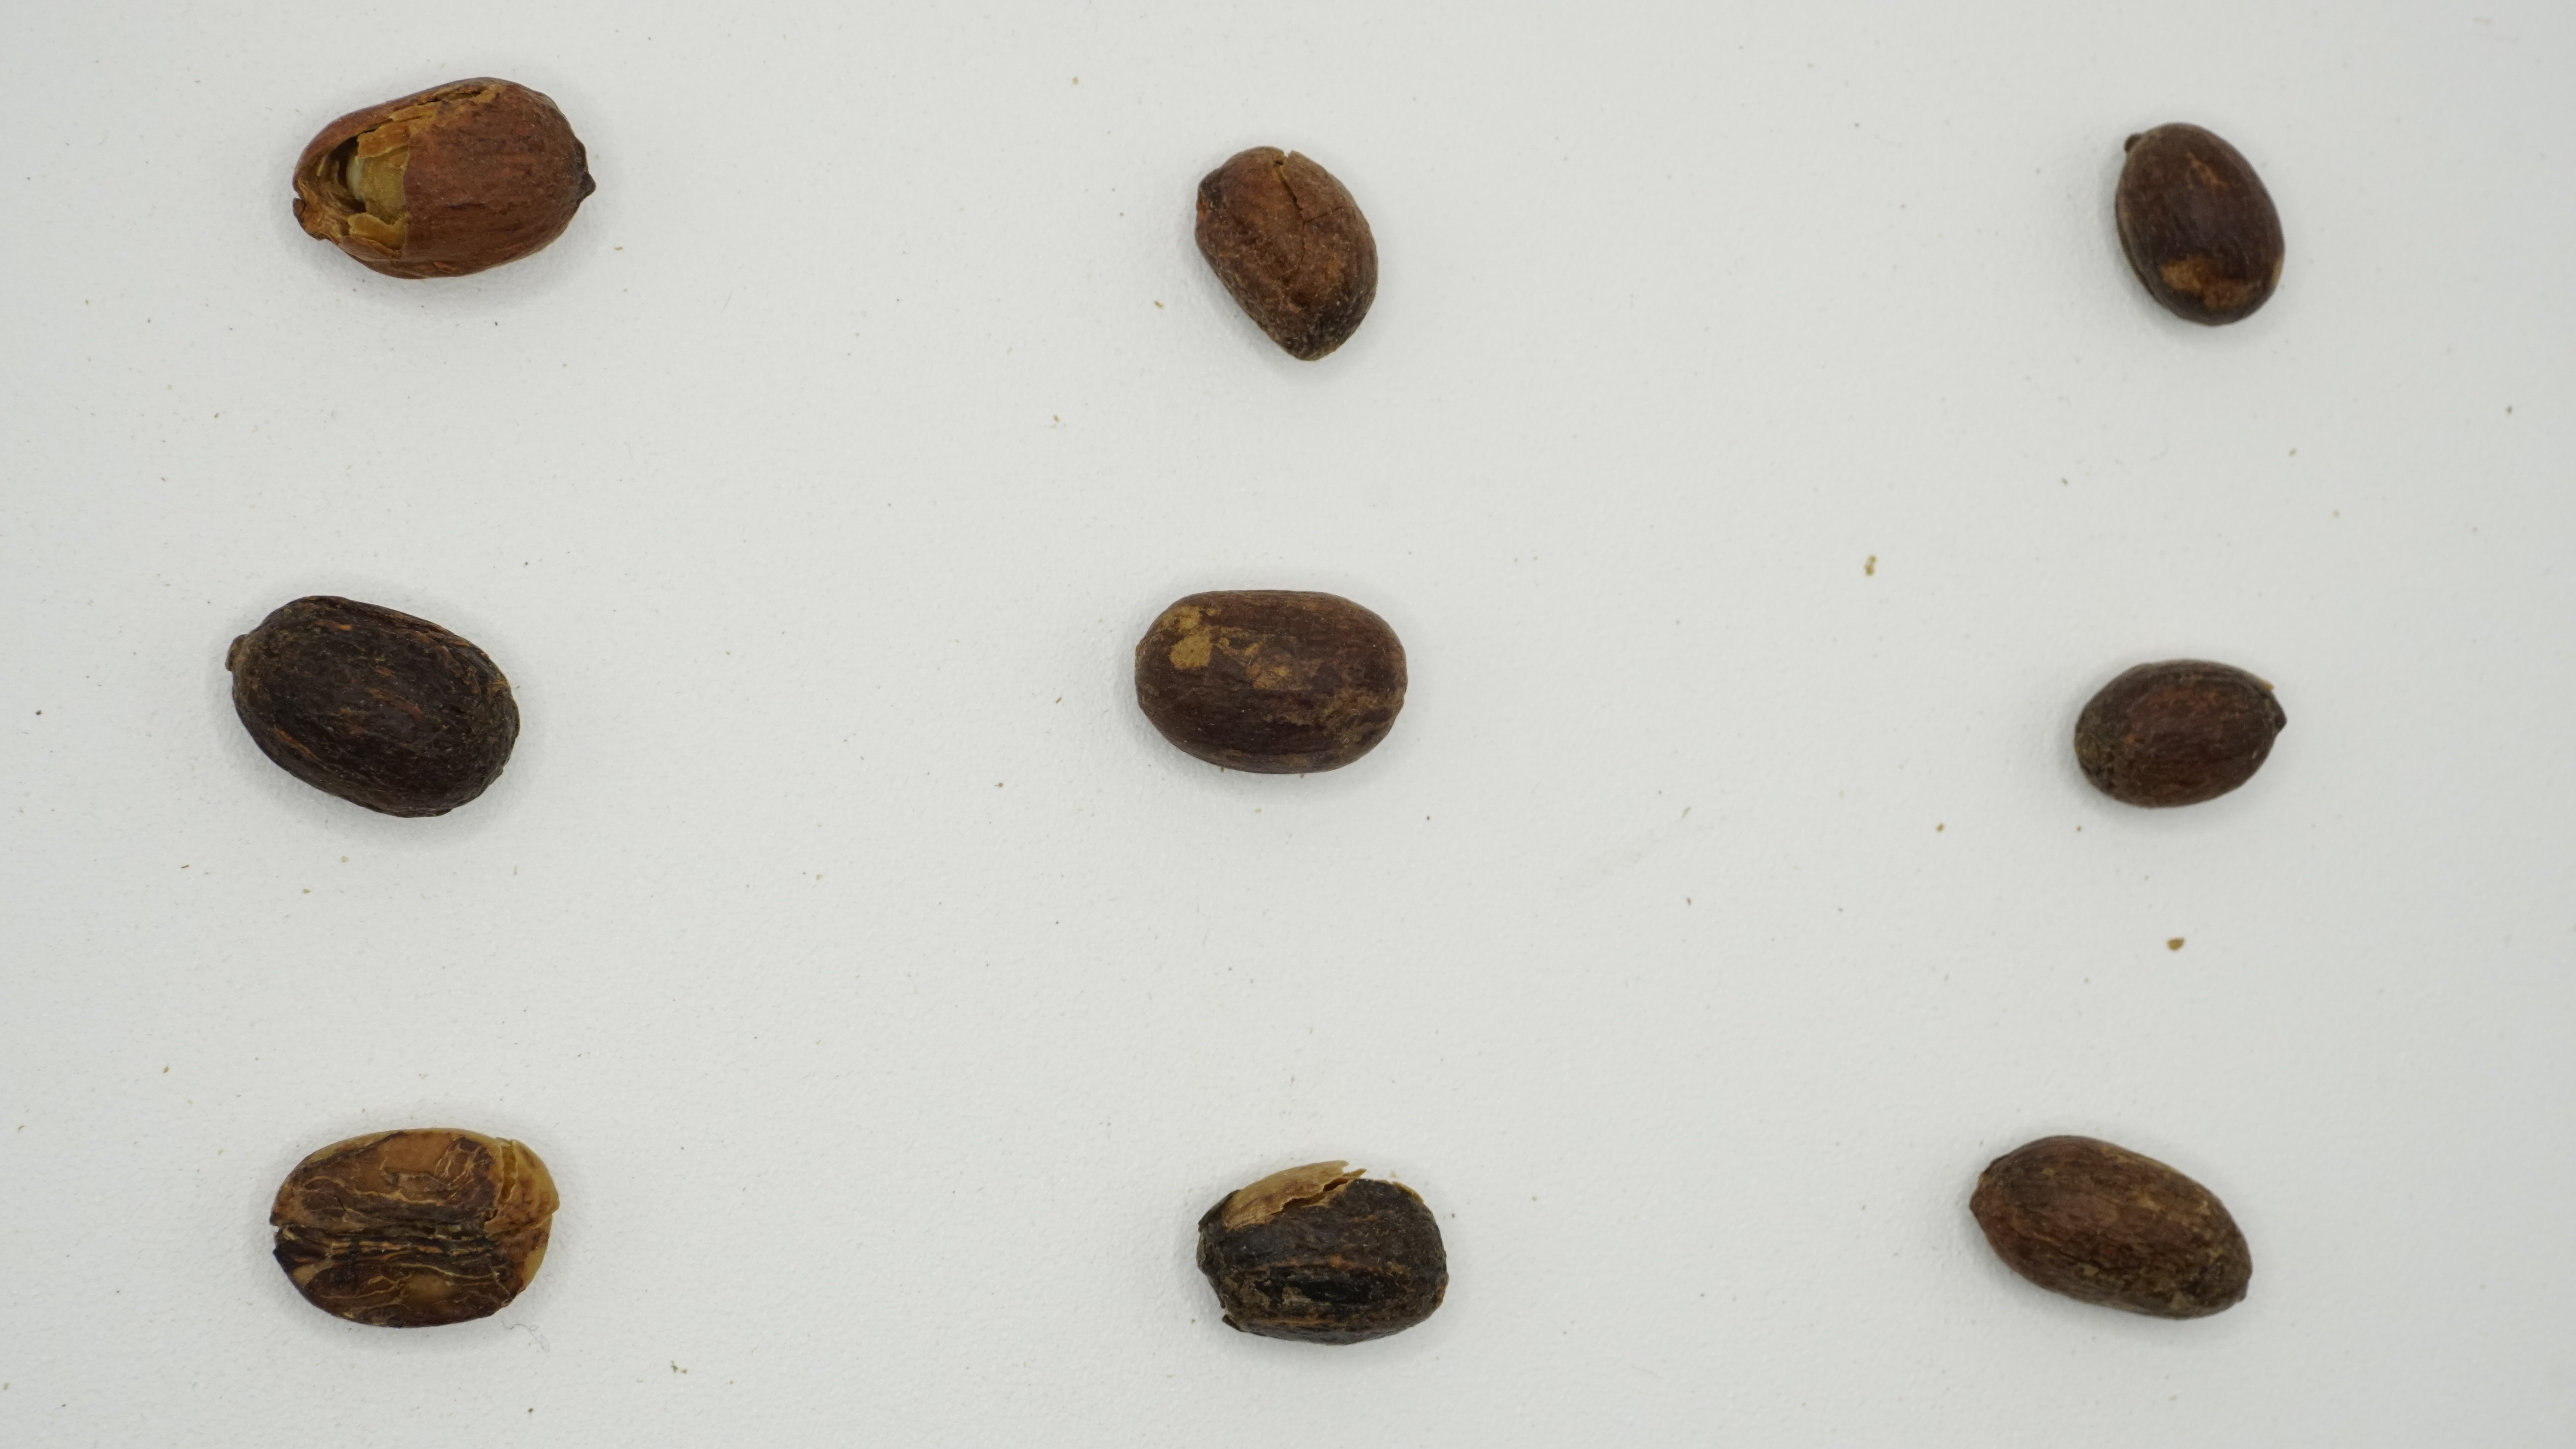
\includegraphics[width=0.3\textwidth]{ch5/1st-Iteration-Table/DriedCherry.JPG} &
		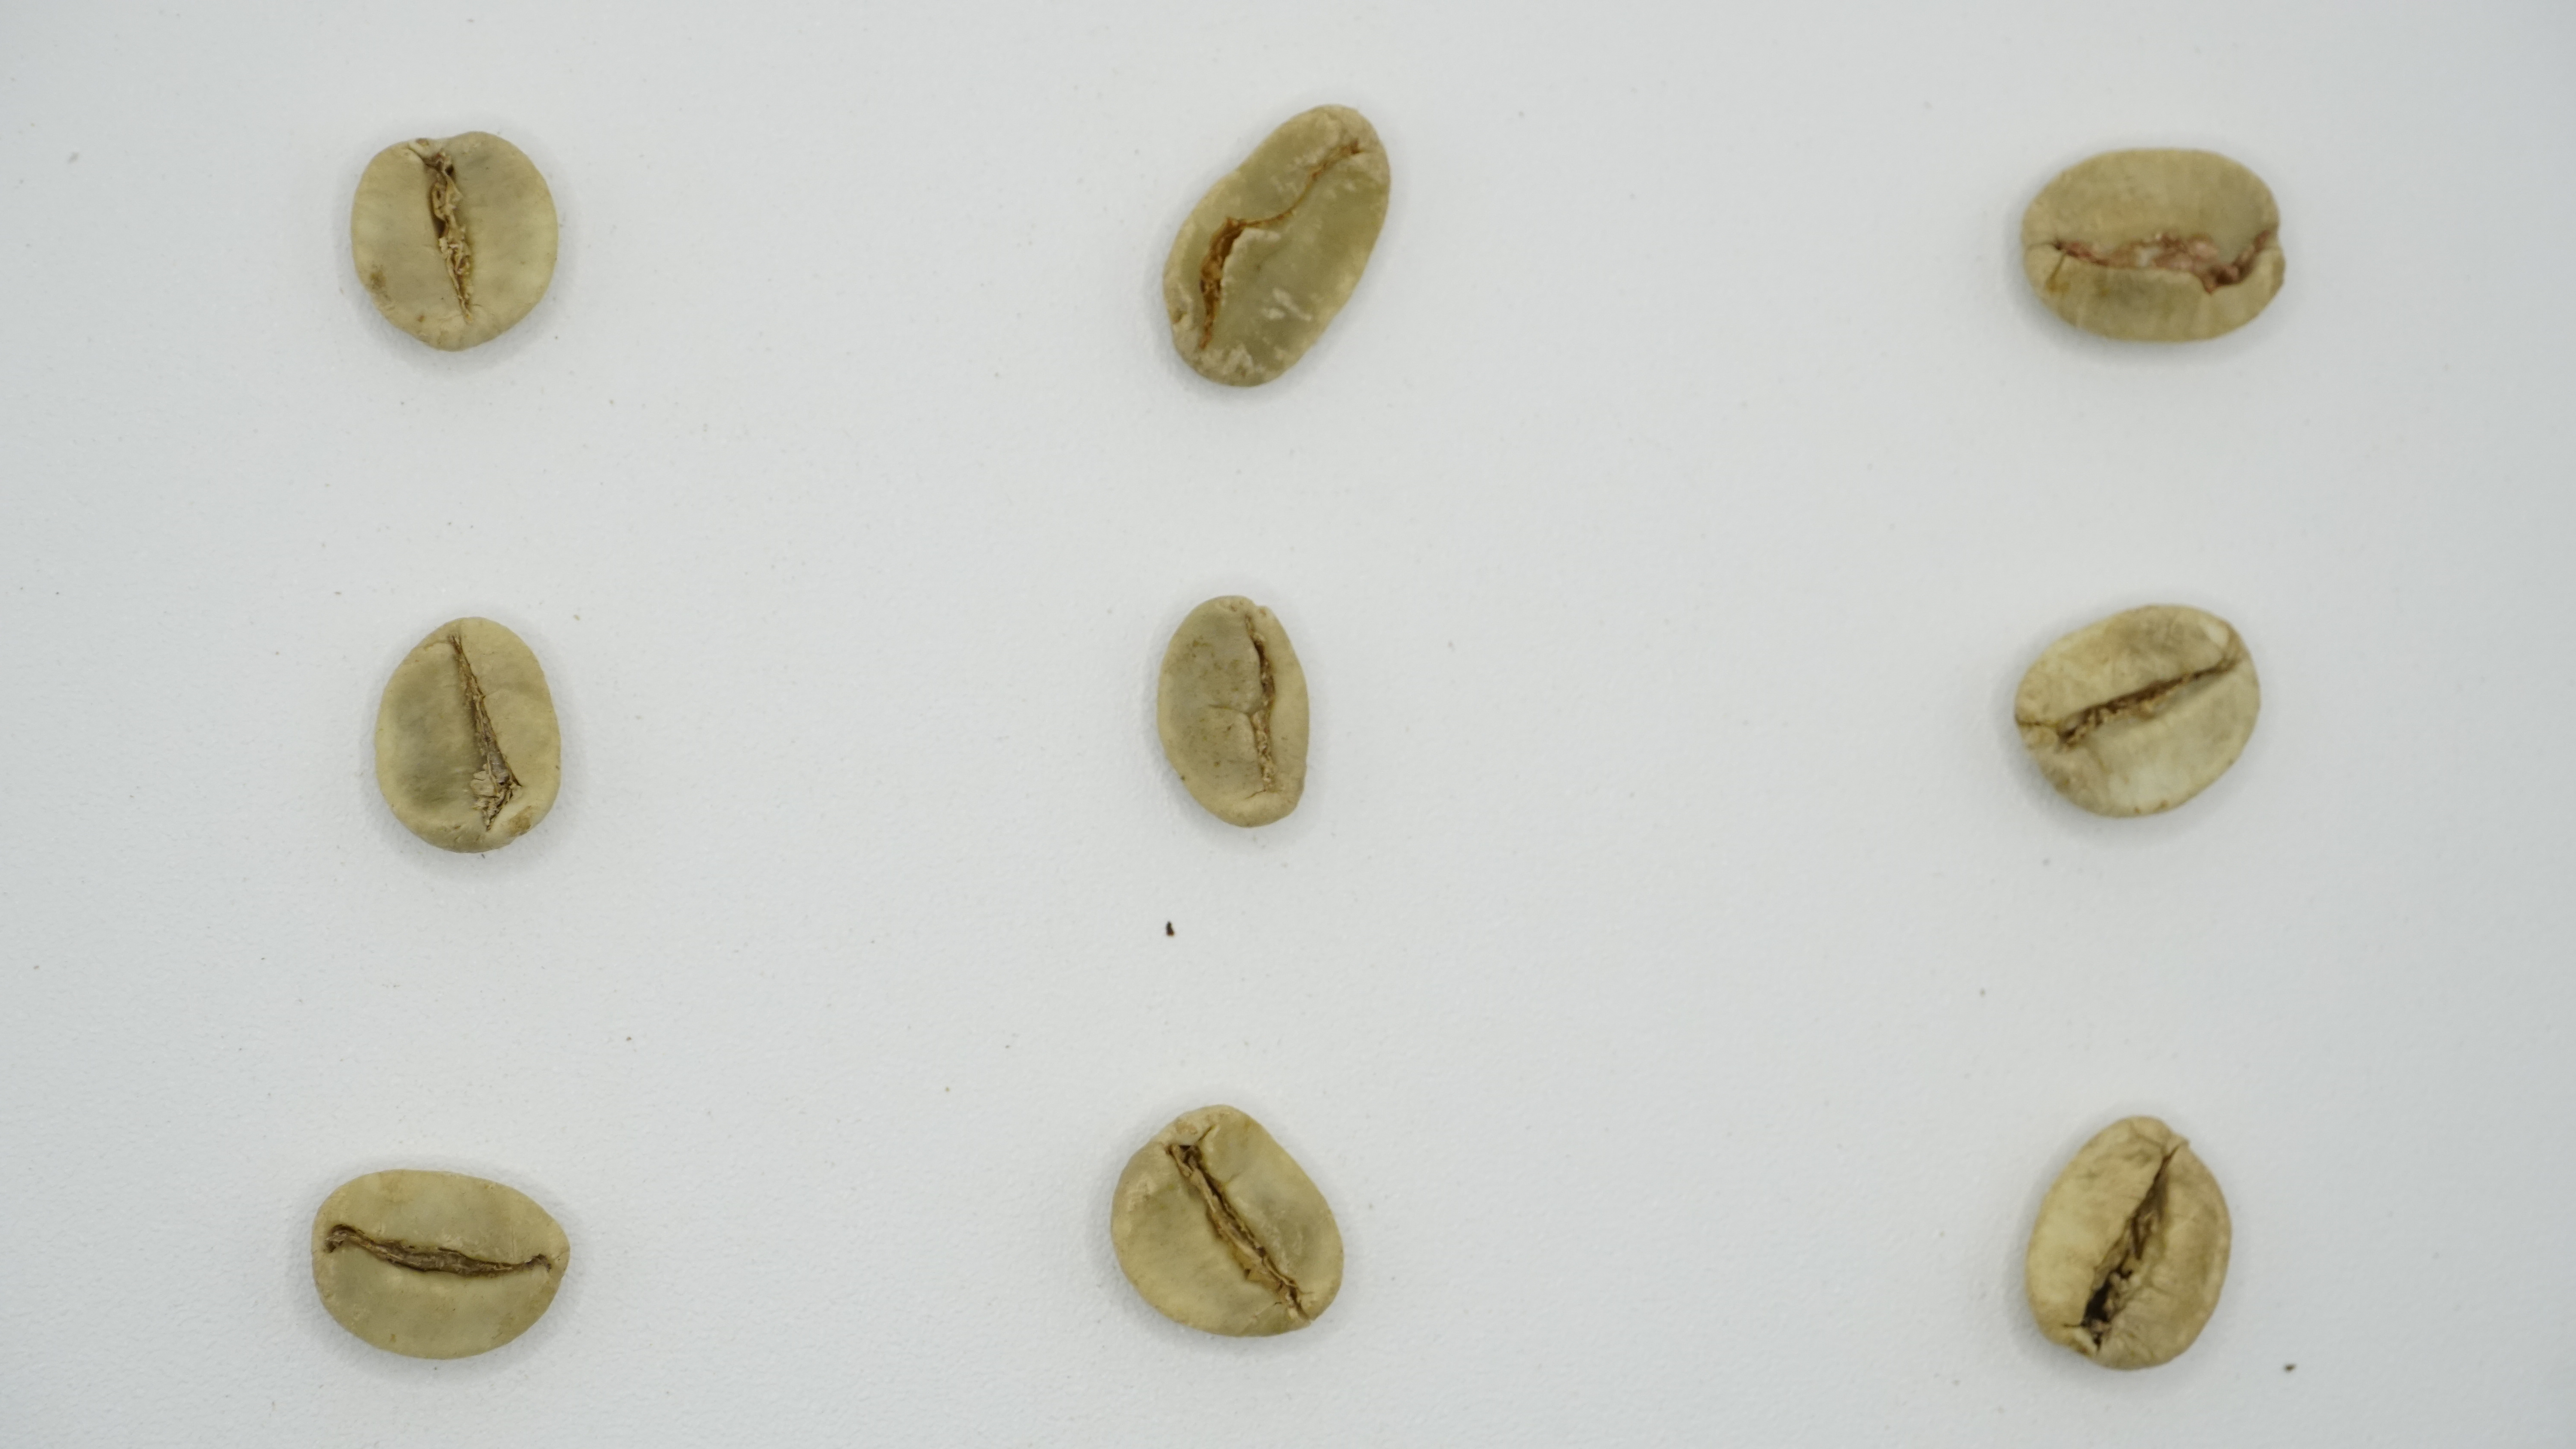
\includegraphics[width=0.3\textwidth]{ch5/1st-Iteration-Table/Floater.JPG} \\
		\textbf{Dried Cherry}  & \textbf{Floater} \\[6pt]
	\end{tabular}
	\begin{tabular}{cc}
		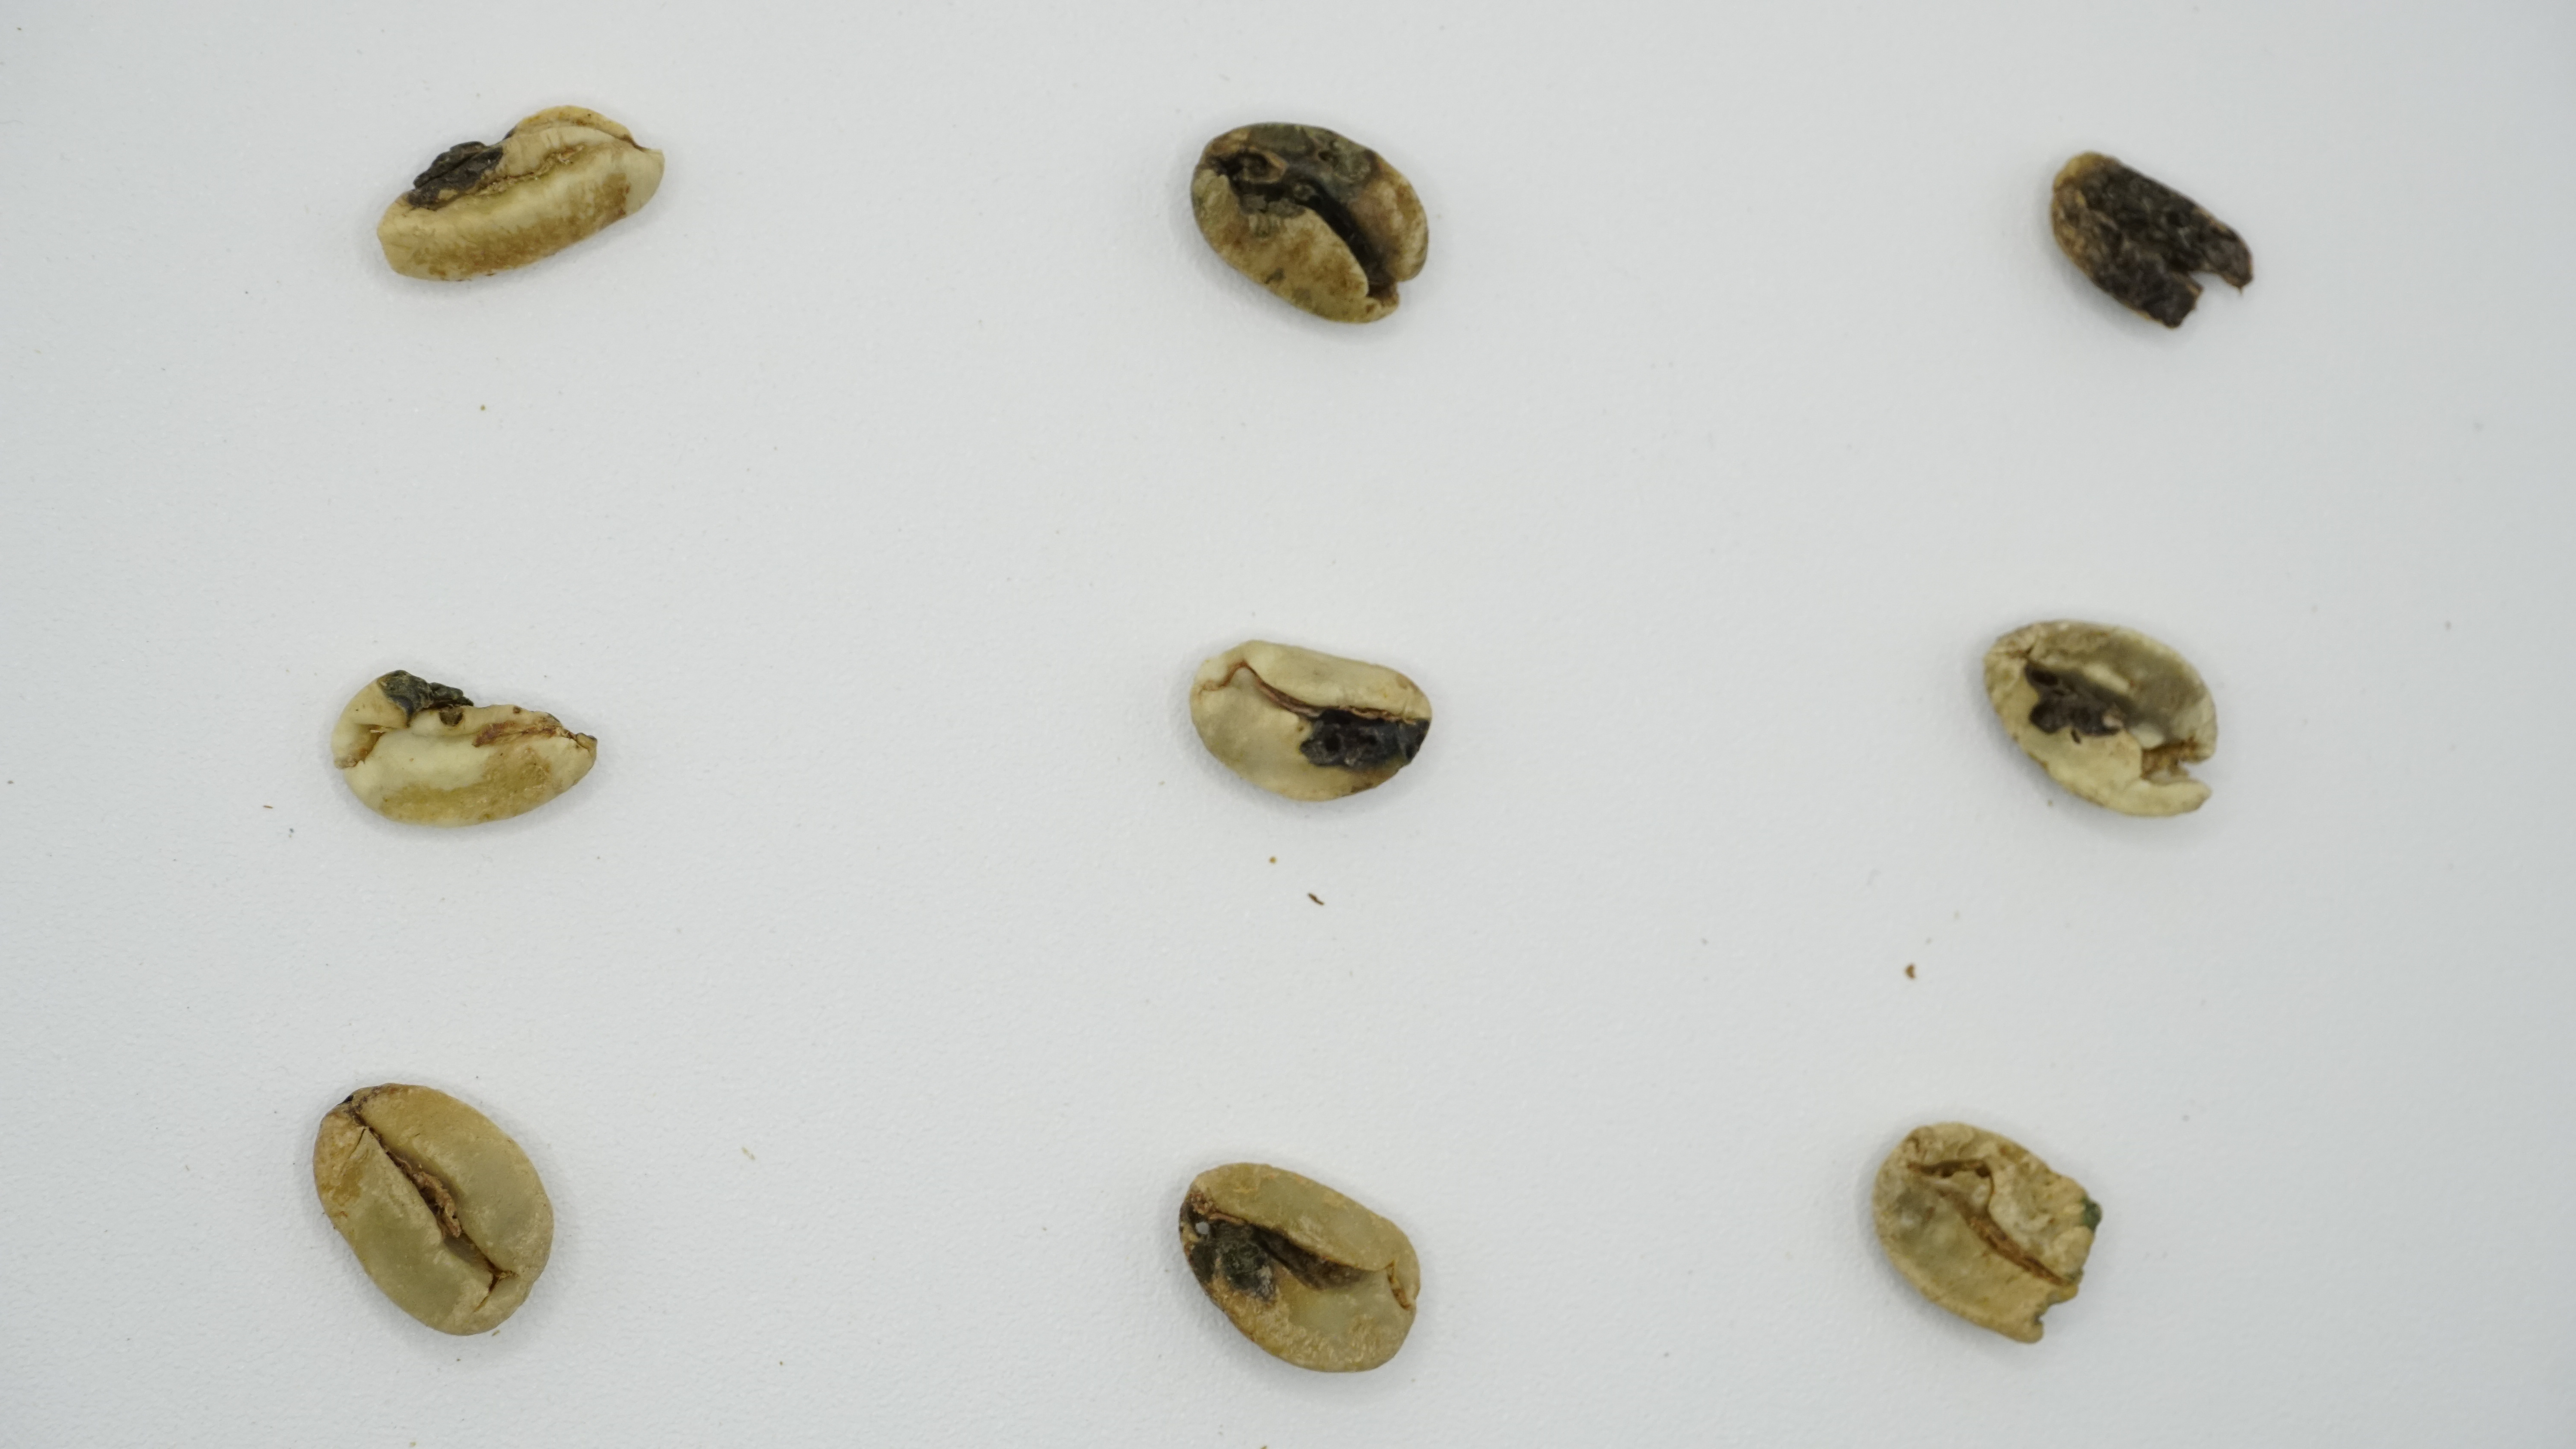
\includegraphics[width=0.3\textwidth]{ch5/1st-Iteration-Table/FungusDamage.JPG} &
		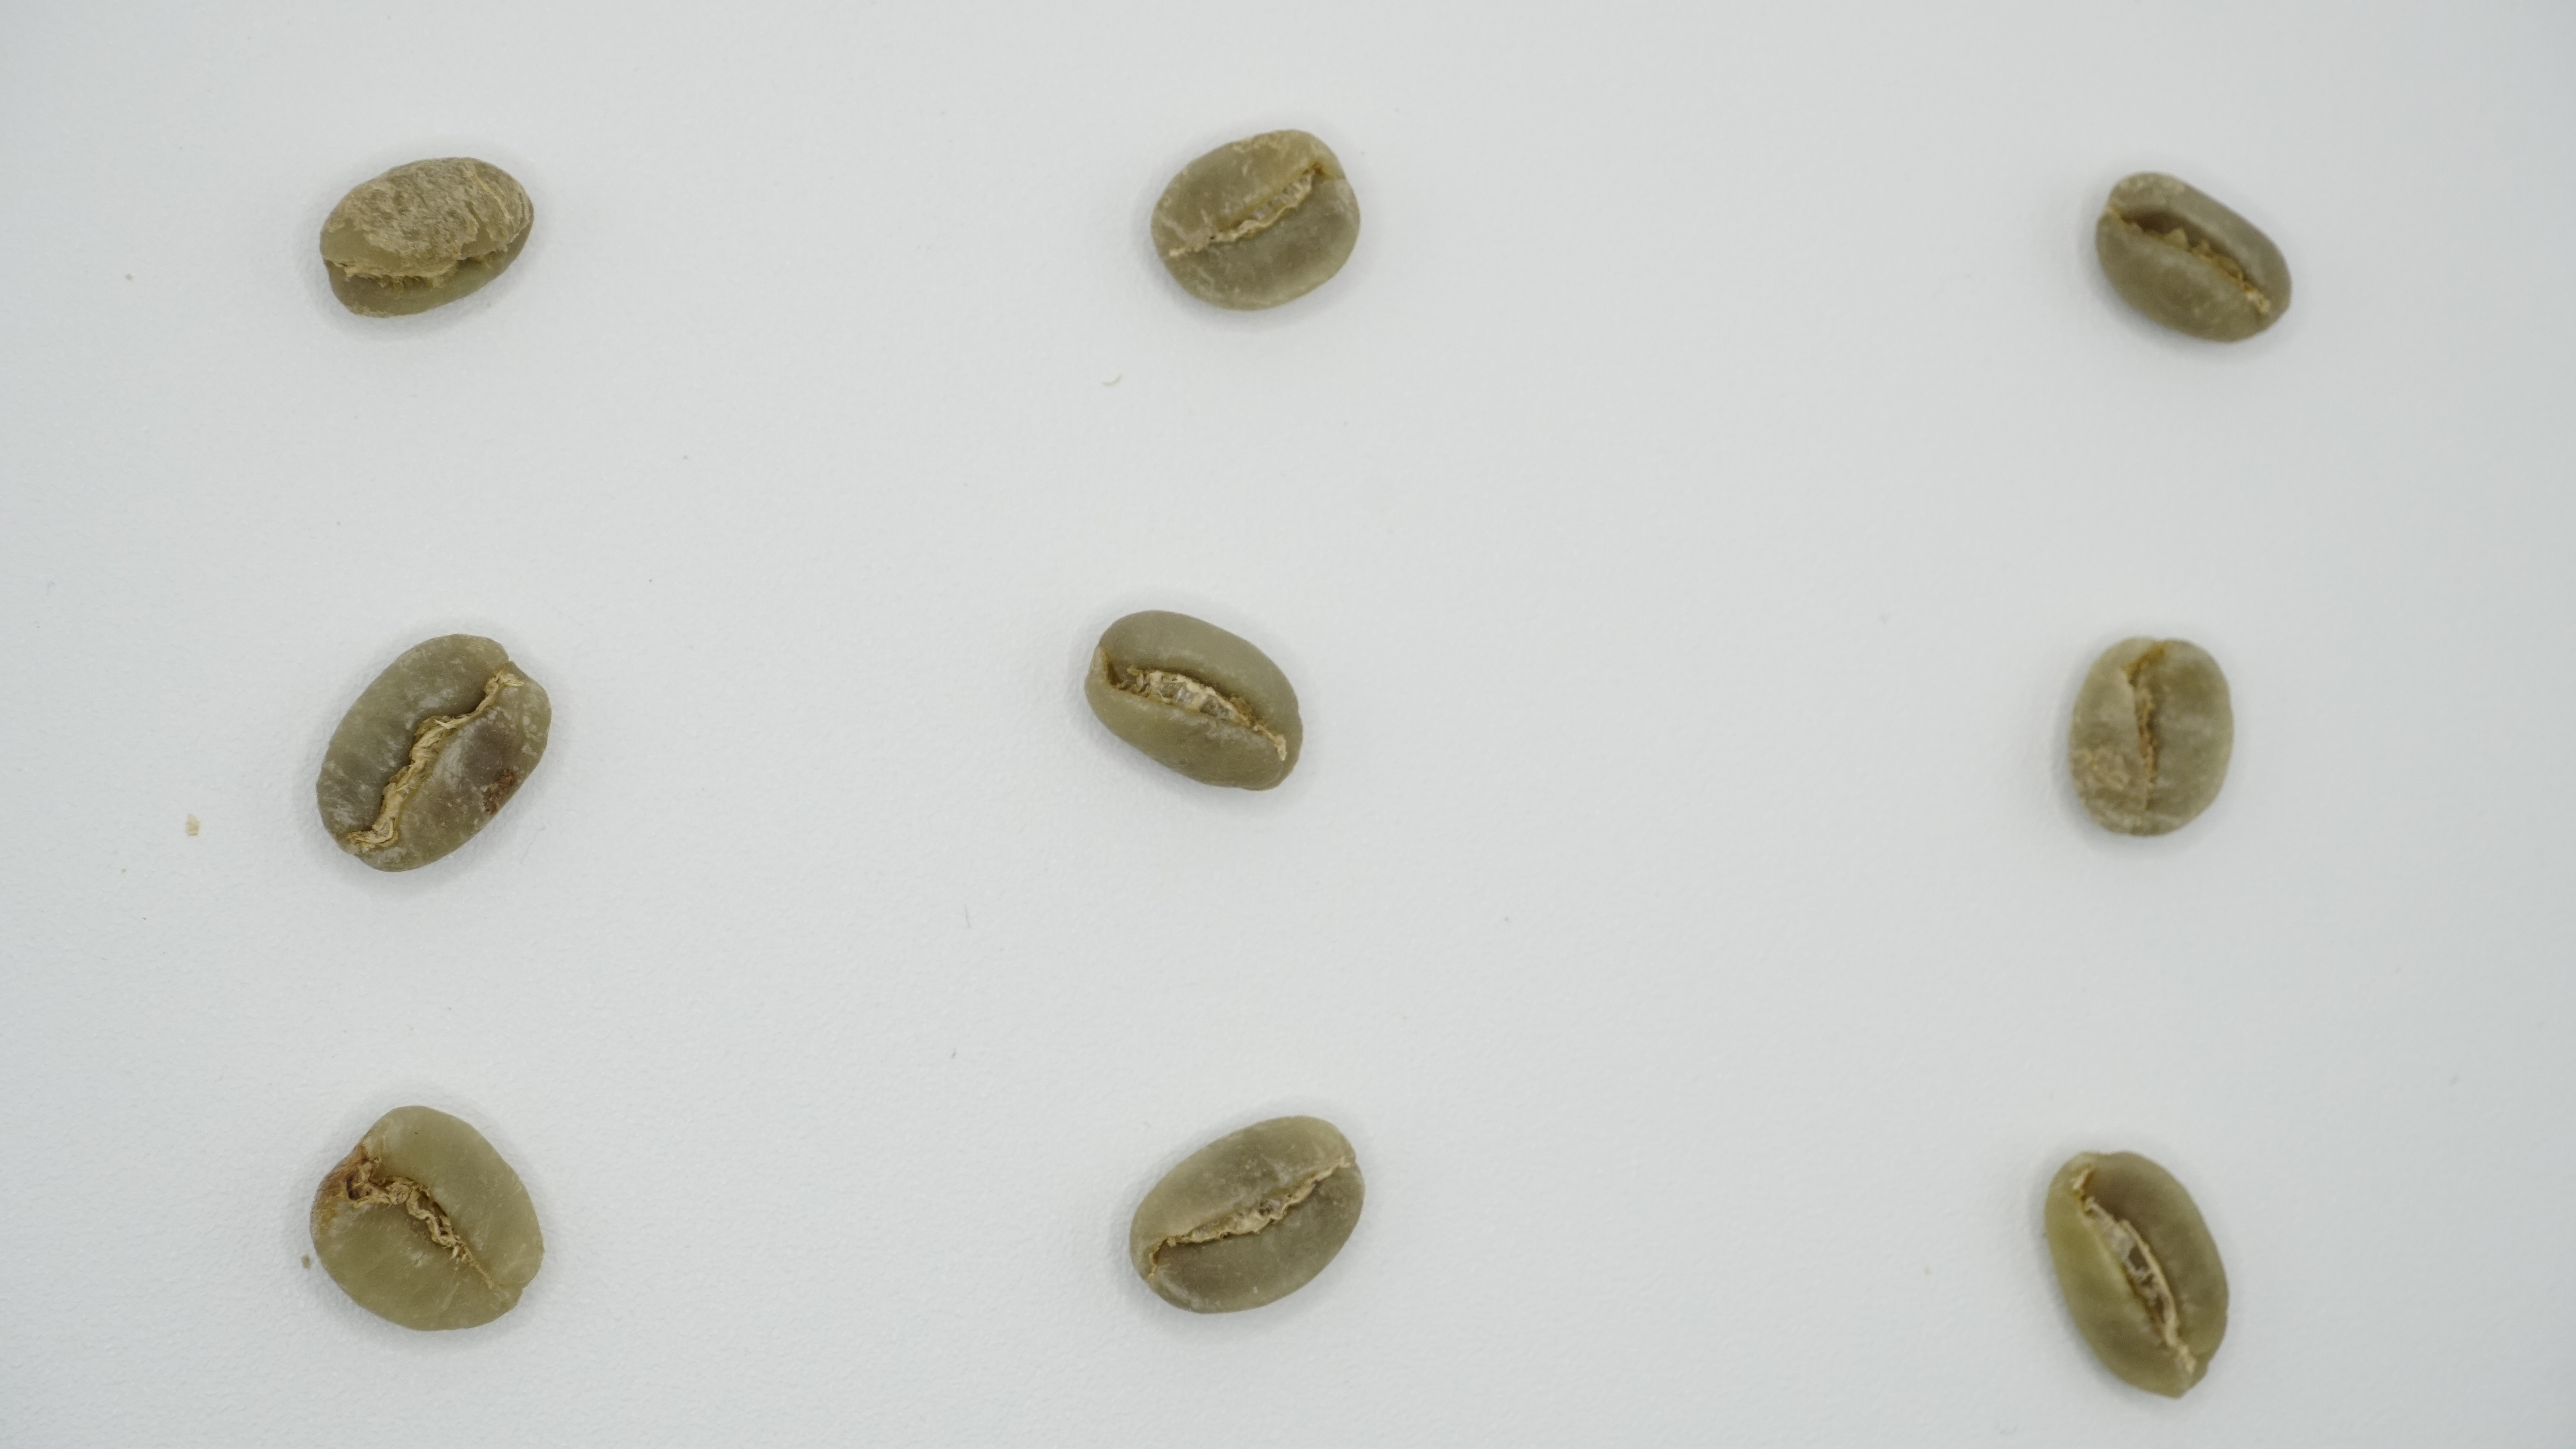
\includegraphics[width=0.3\textwidth]{ch5/1st-Iteration-Table/Good.JPG} \\
		\textbf{Fungus Damage}  & \textbf{Good} \\[6pt]
	\end{tabular}
	\begin{tabular}{cc}
		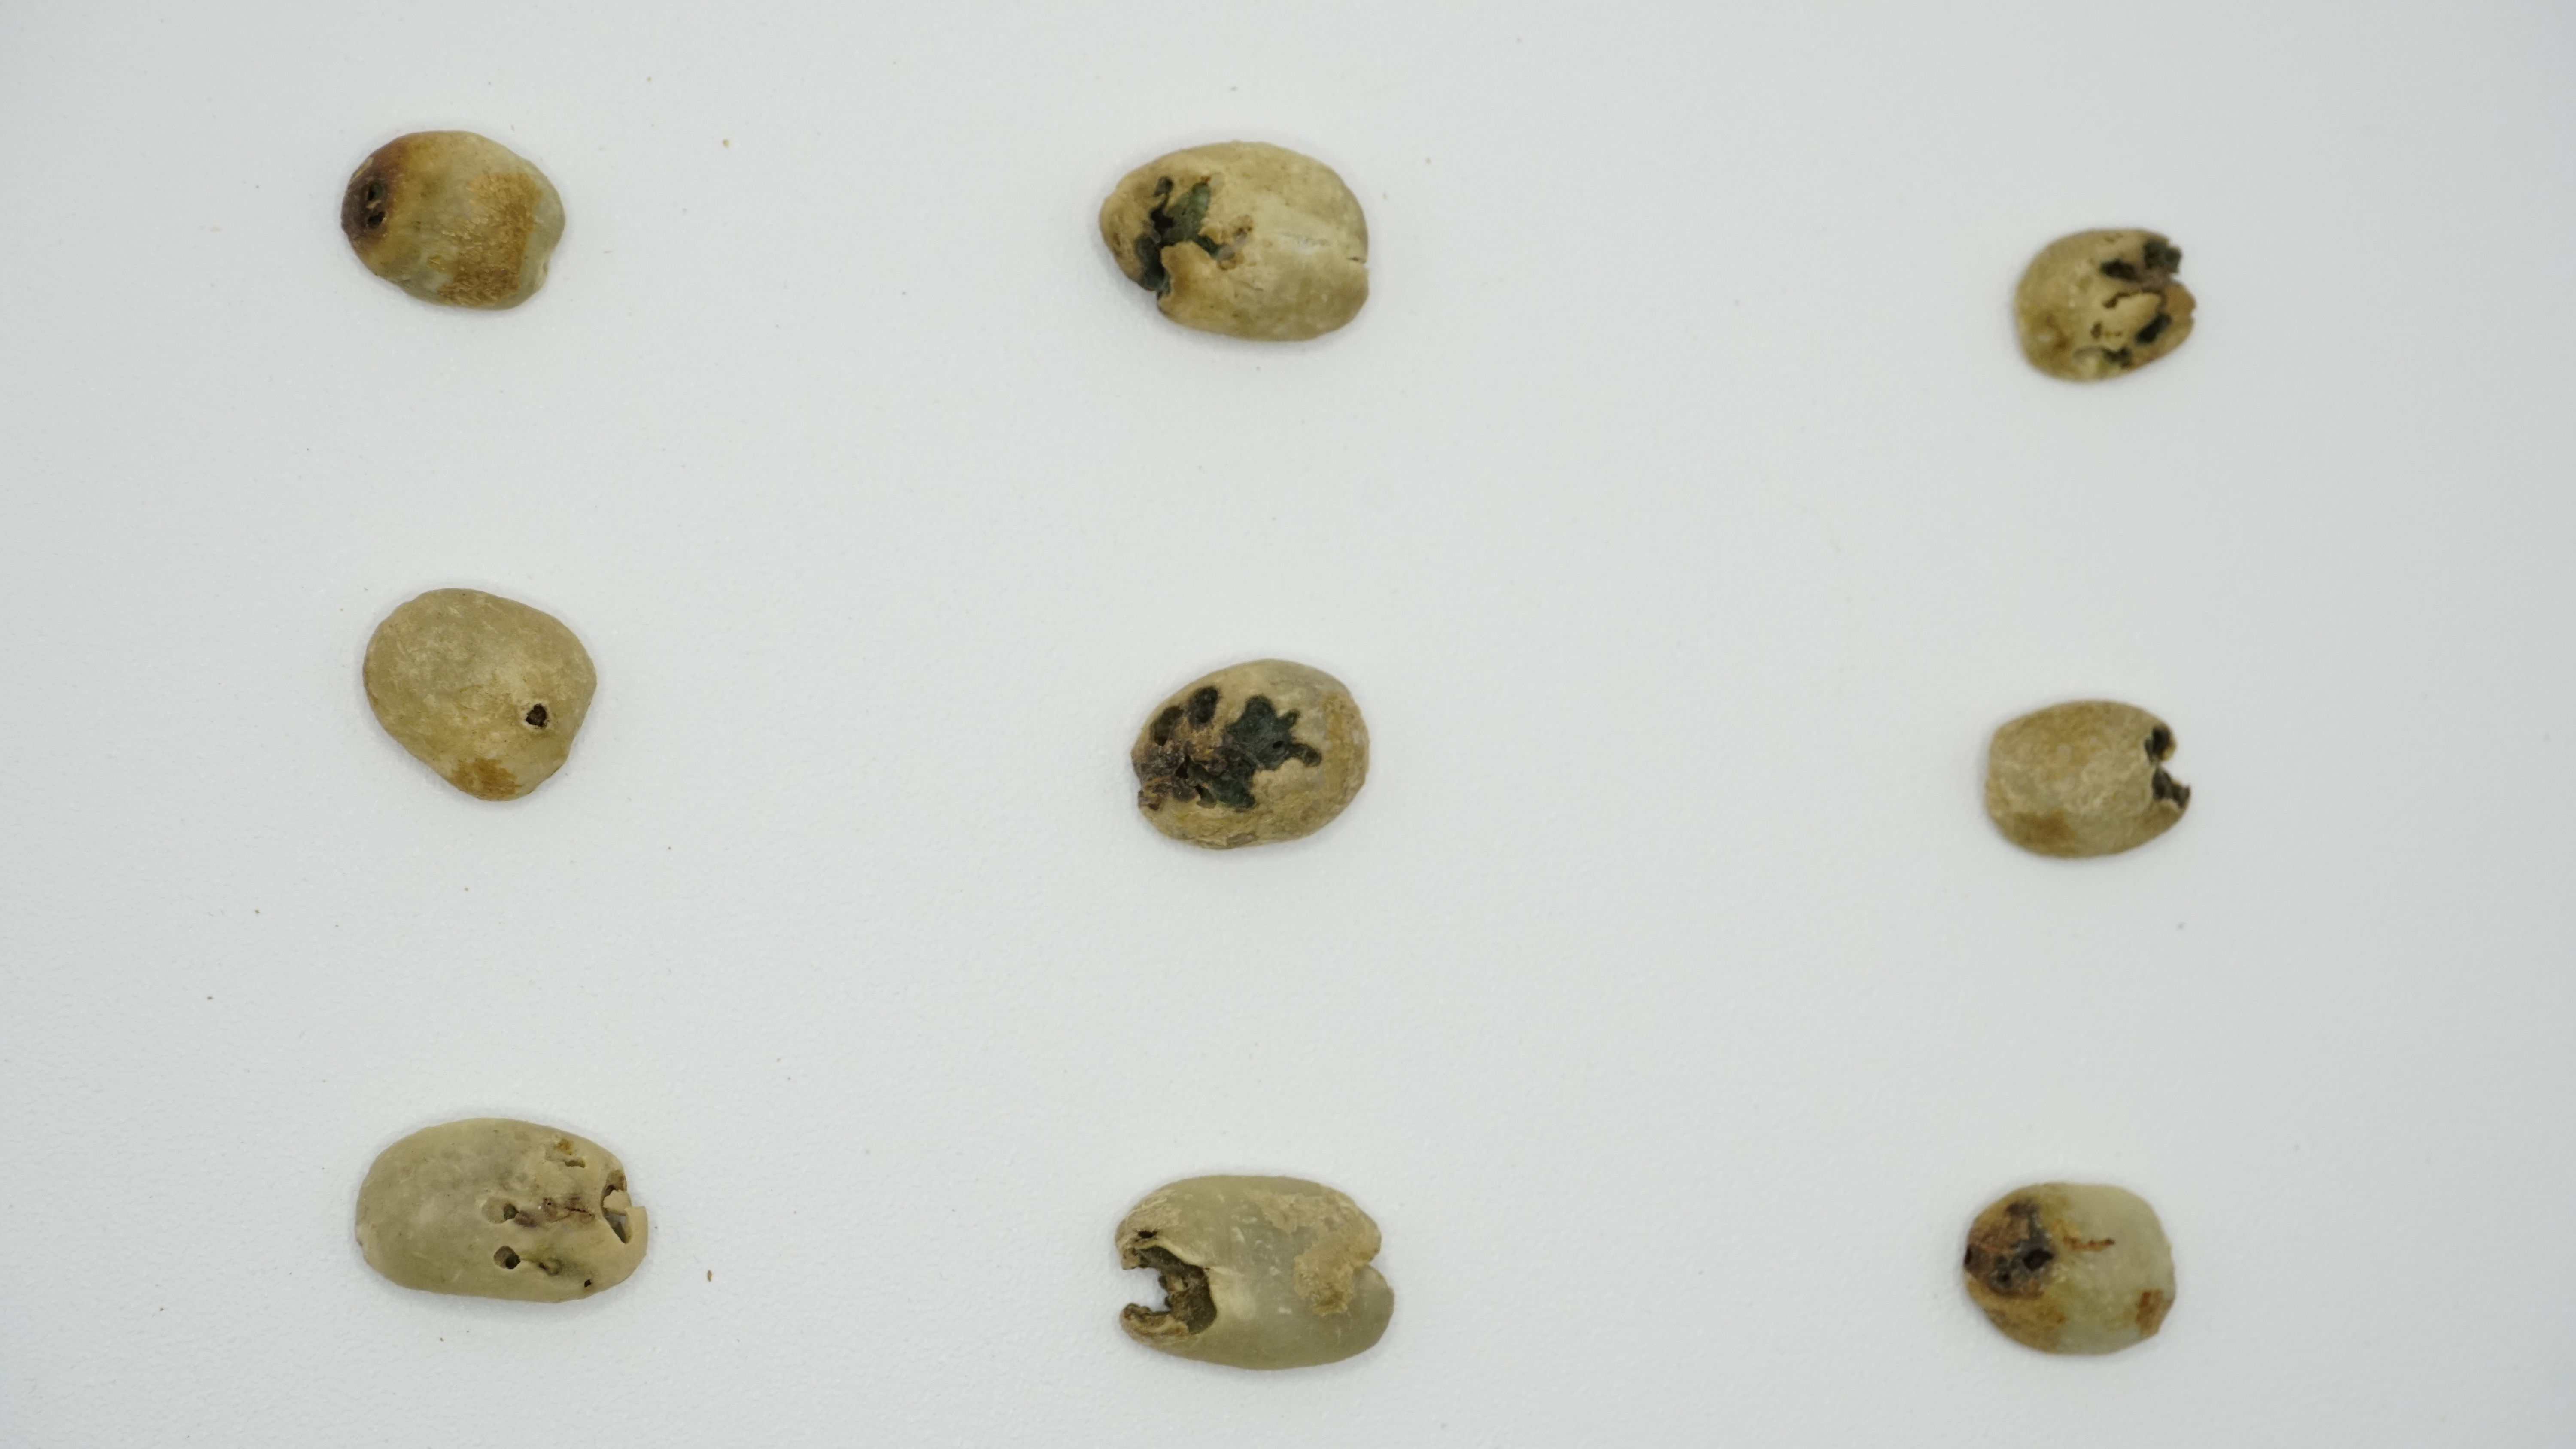
\includegraphics[width=0.3\textwidth]{ch5/1st-Iteration-Table/InsectDamage.JPG} &
		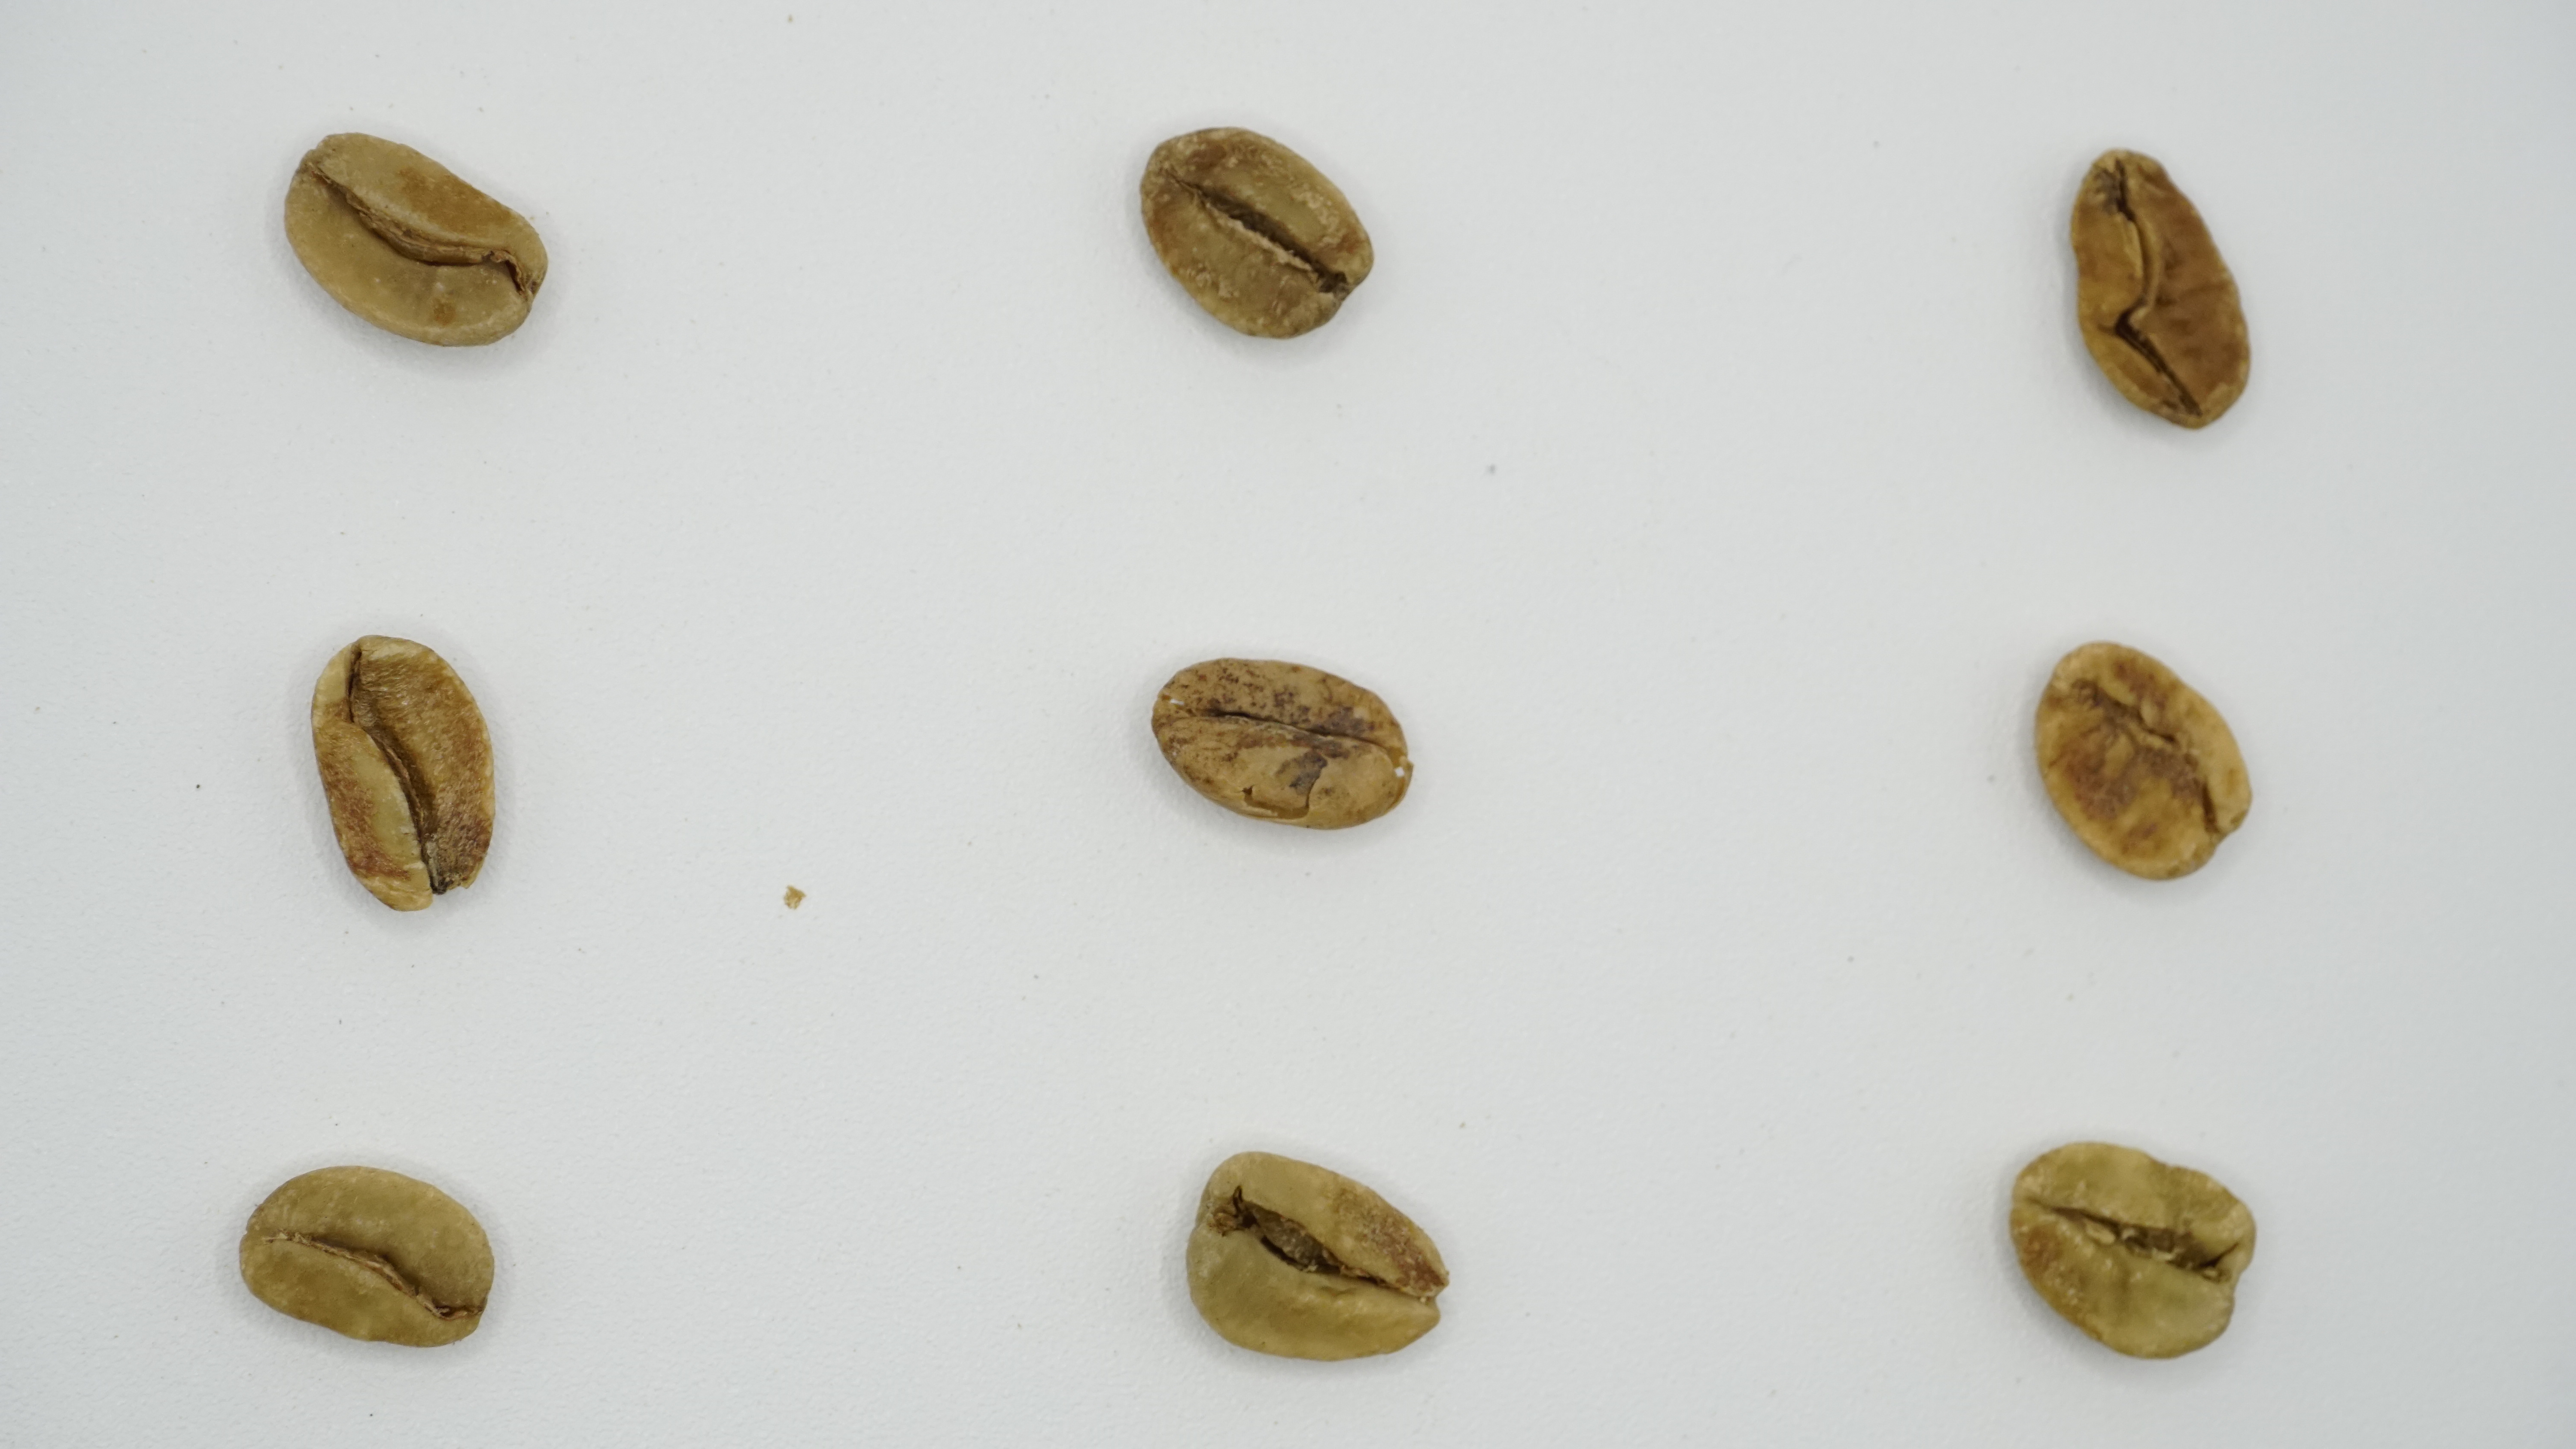
\includegraphics[width=0.3\textwidth]{ch5/1st-Iteration-Table/Sour.JPG} \\
		\textbf{Insect Damage}  & \textbf{Sour} \\[6pt]
	\end{tabular}
	\caption{Sample Images from the First Iteration of Dataset Collection}
\end{figure}


The first iteration of data collection utilized a Sony A6300 camera with its Kit Lens, set at 1/200 Shutter Speed, 1000 ISO, and a Distance of 50mm. The beans were captured in batches of nine, carefully arranged within the camera's field of view following the rule of thirds. The rule of thirds is a photographic composition principle where an image is divided into a 3x3 grid, creating nine equal grid lines to create balance to the photo. By aligning the coffee beans with the rule of thirds, the group ensured a structured and even distribution of the beans within the frame. This setup also made it easier to automate the cropping process, as the predefined positions of the beans allowed a Python script to accurately extract individual images.

\subsection{Second Iteration of Dataset Collection}
\begin{figure}[H]
	\centering
	\begin{tabular}{cc}
		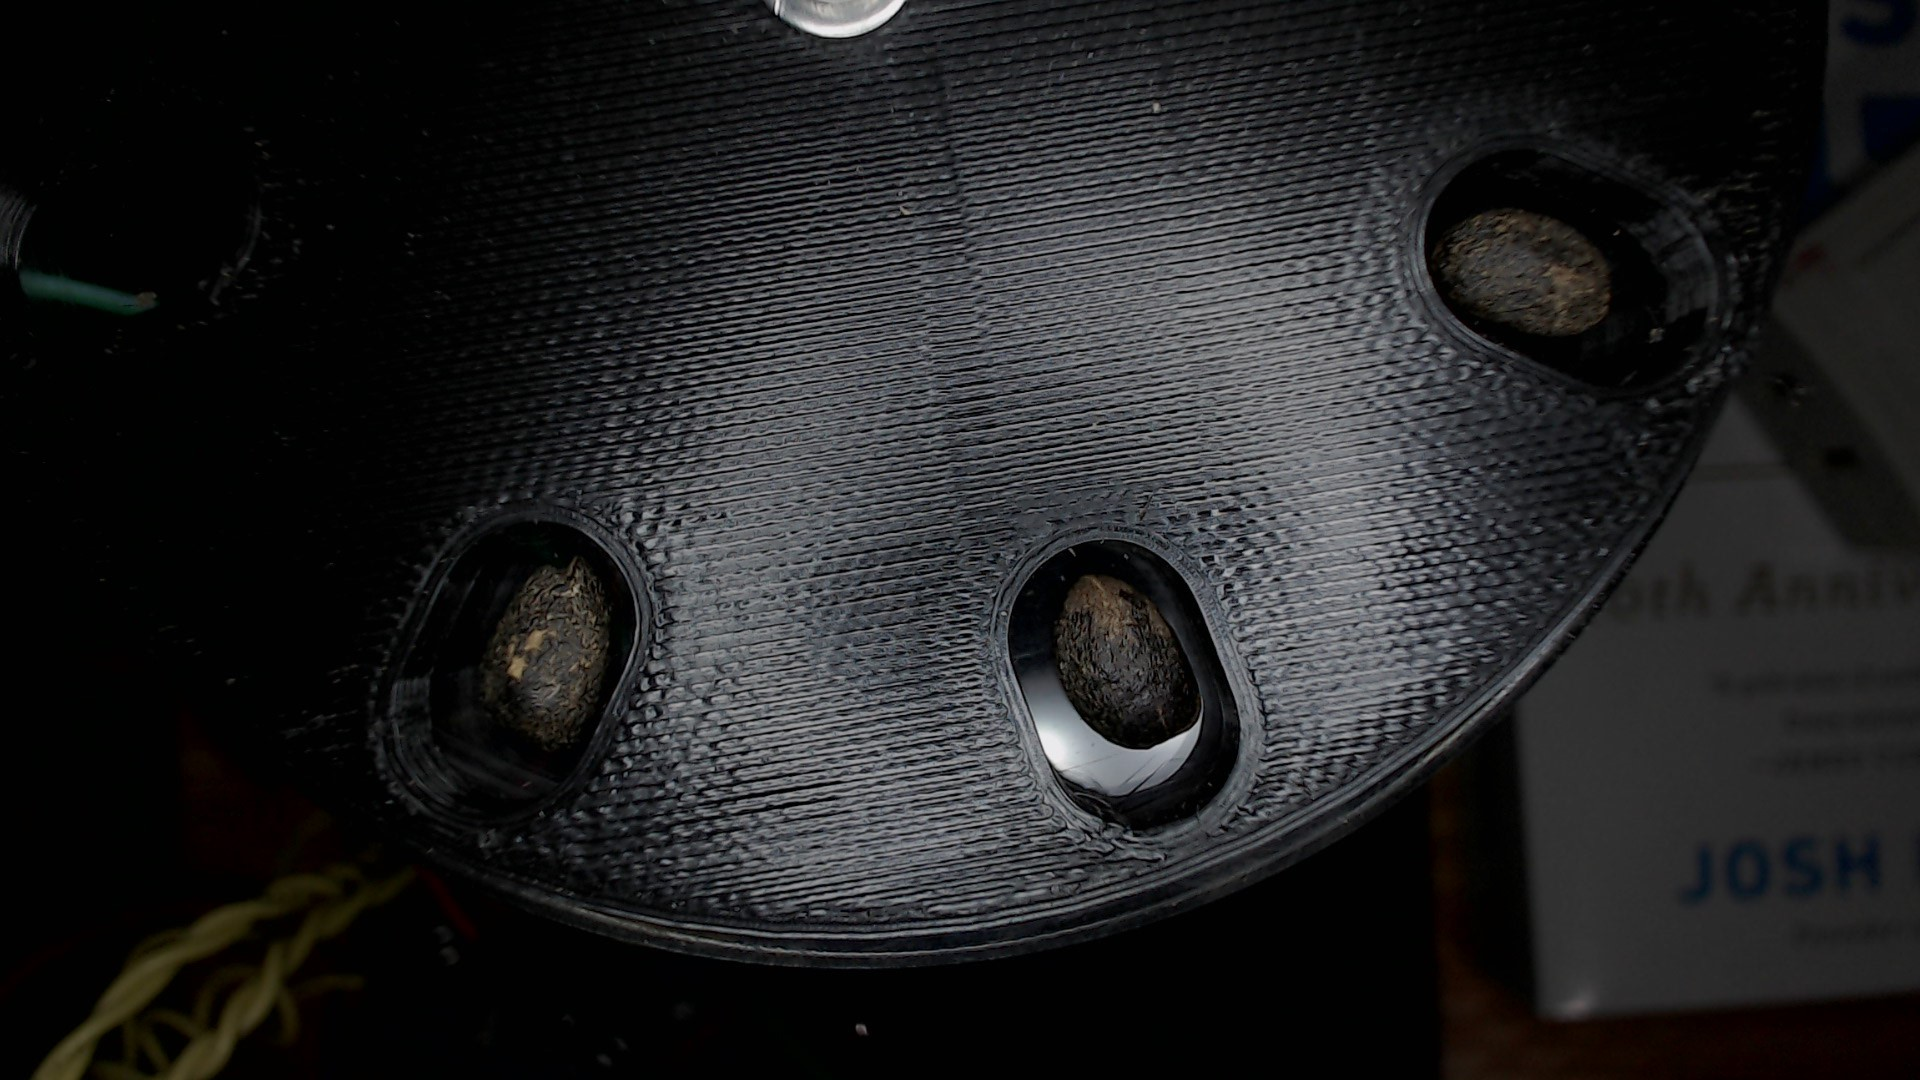
\includegraphics[width=0.3\textwidth]{ch5/2nd-Iteration-Table/Black.jpg} &
		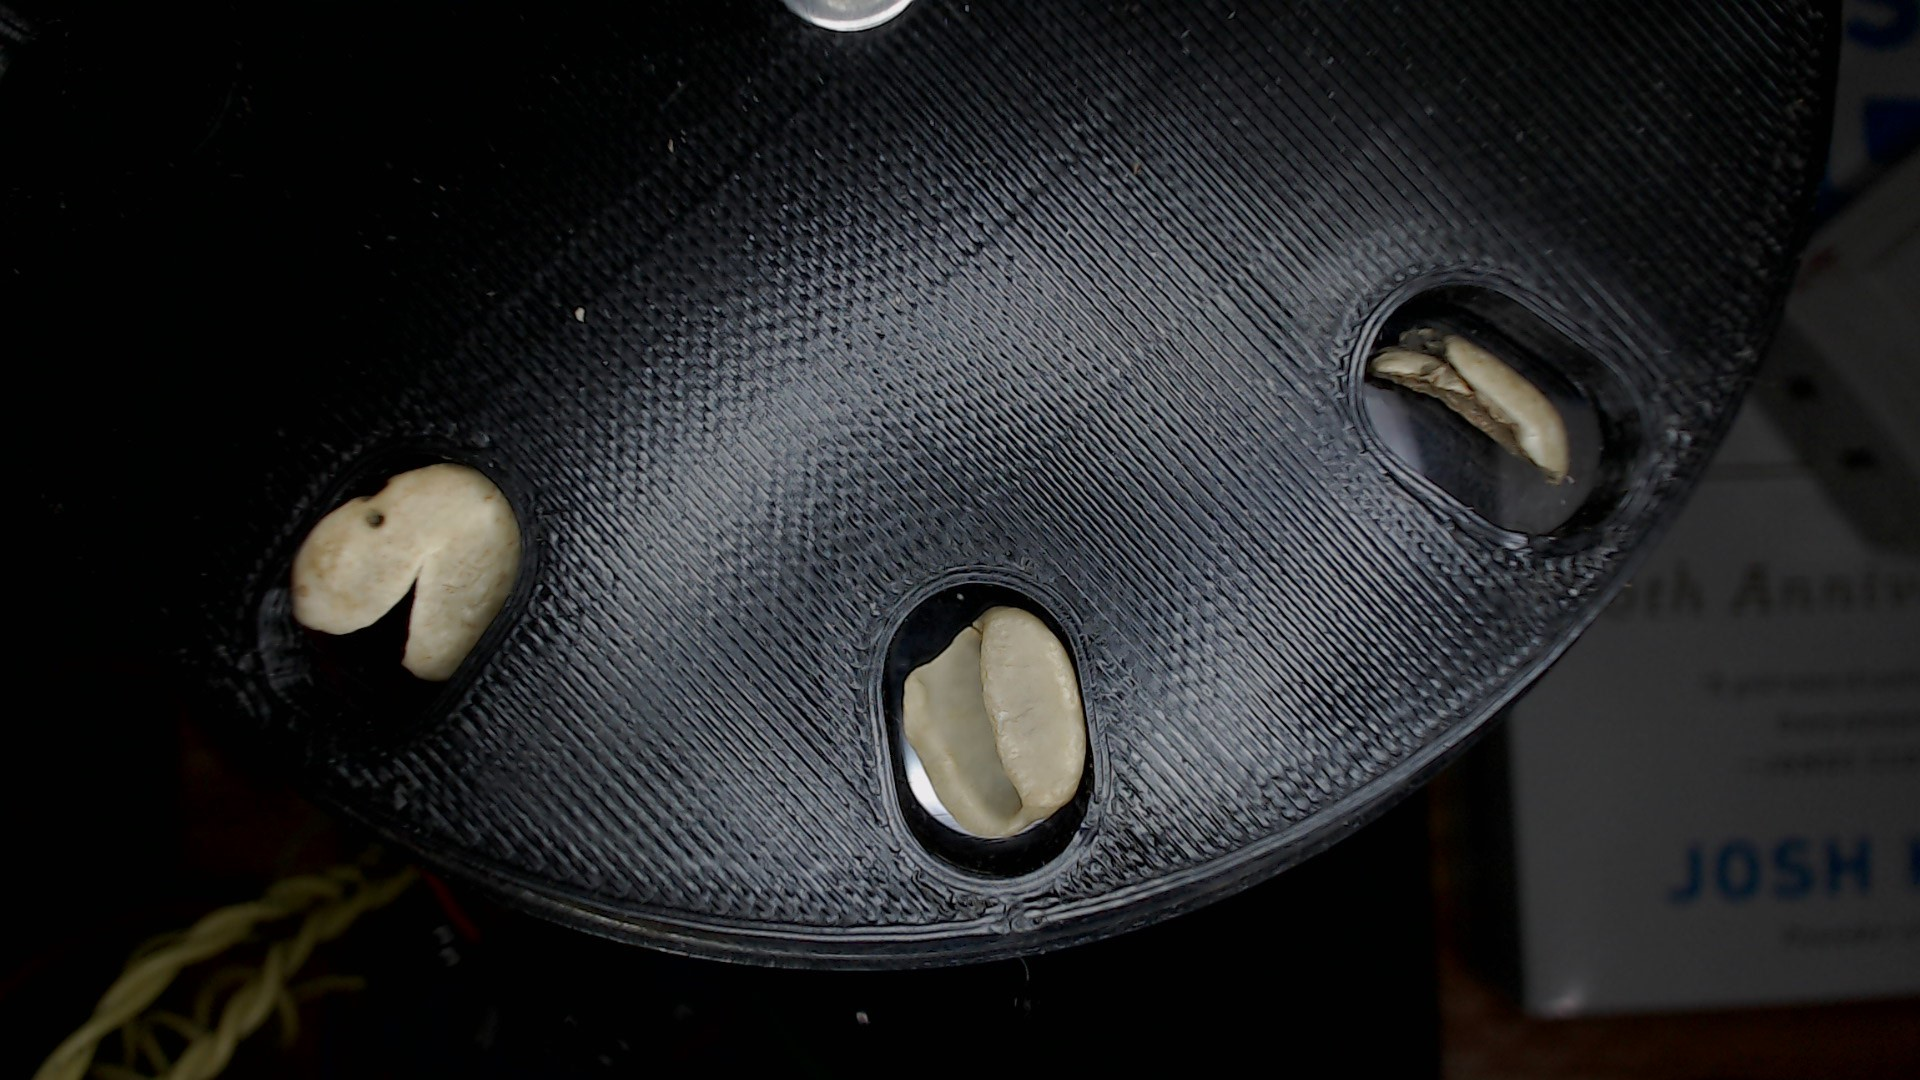
\includegraphics[width=0.3\textwidth]{ch5/2nd-Iteration-Table/Broken.jpg} \\
		\textbf{Black}  & \textbf{Broken} \\[6pt]
	\end{tabular}
	\begin{tabular}{cc}
		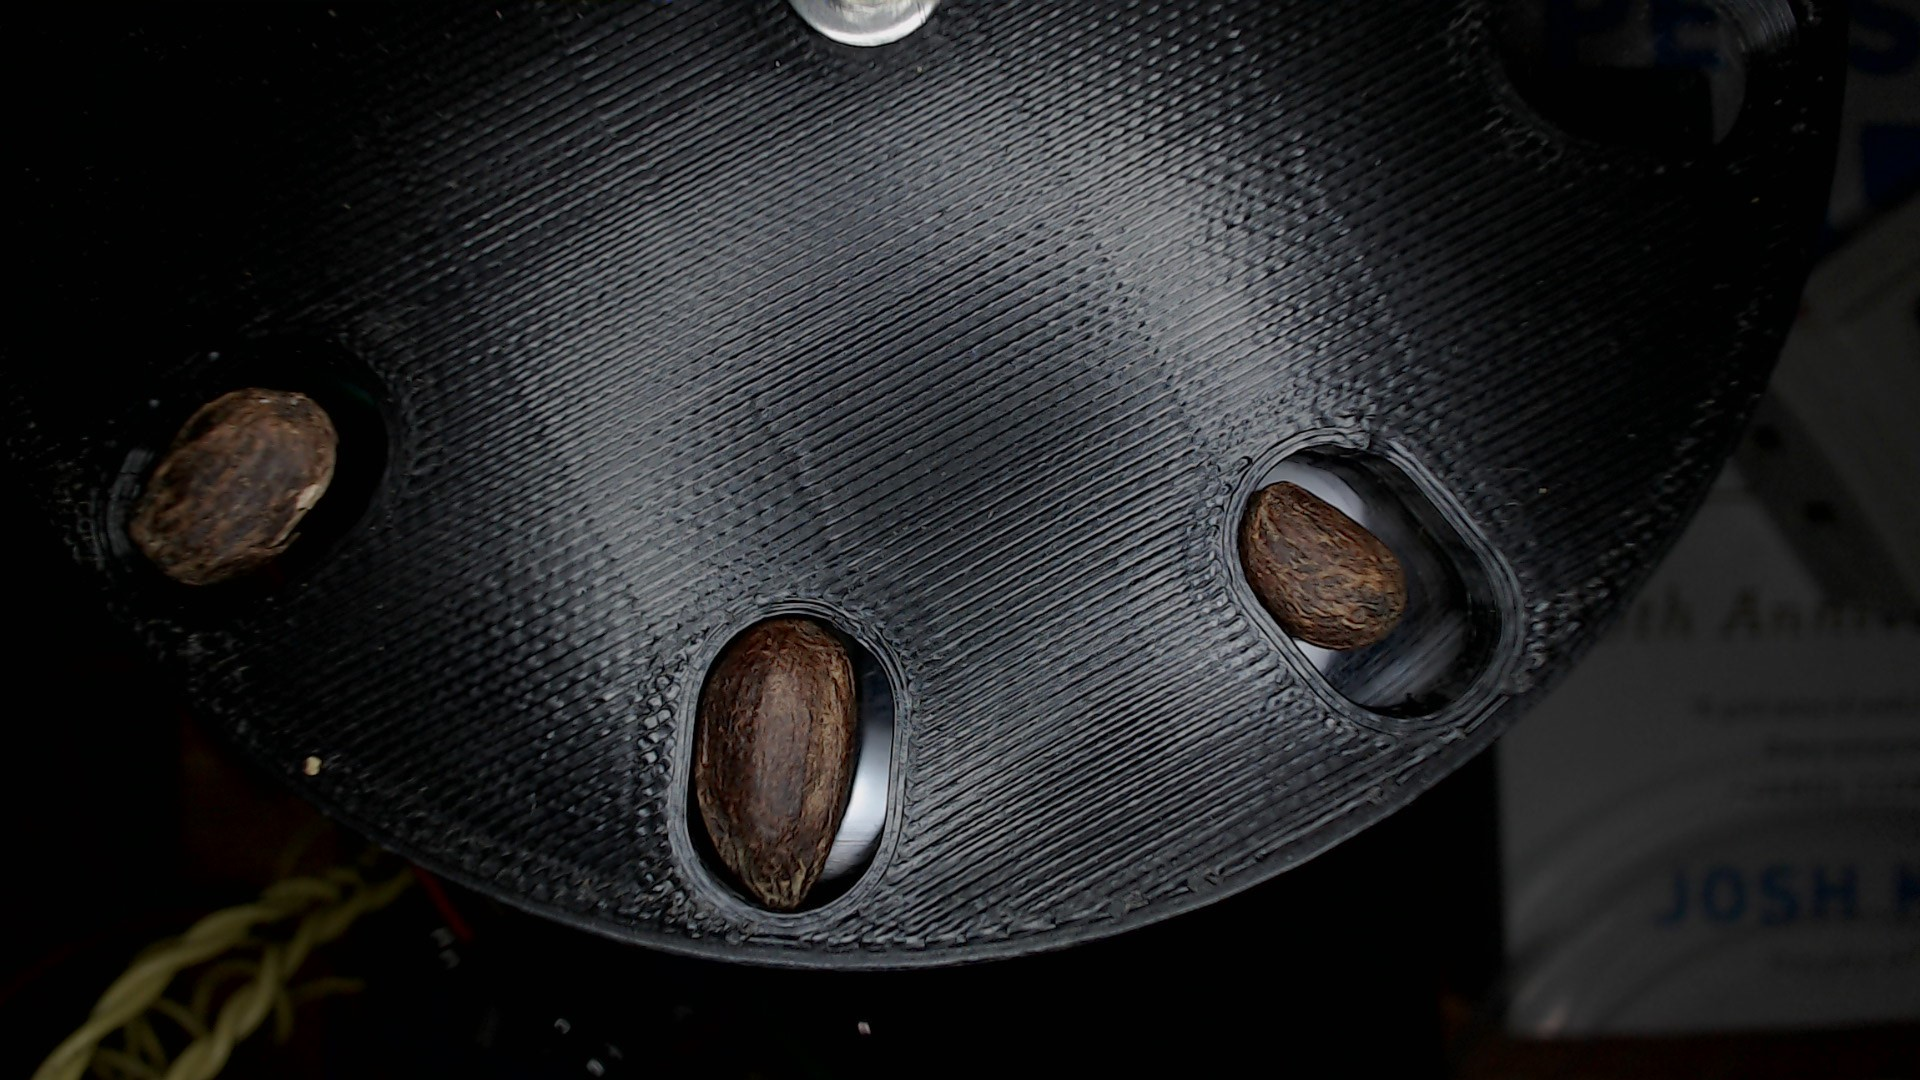
\includegraphics[width=0.3\textwidth]{ch5/2nd-Iteration-Table/DriedCherry.jpg} &
		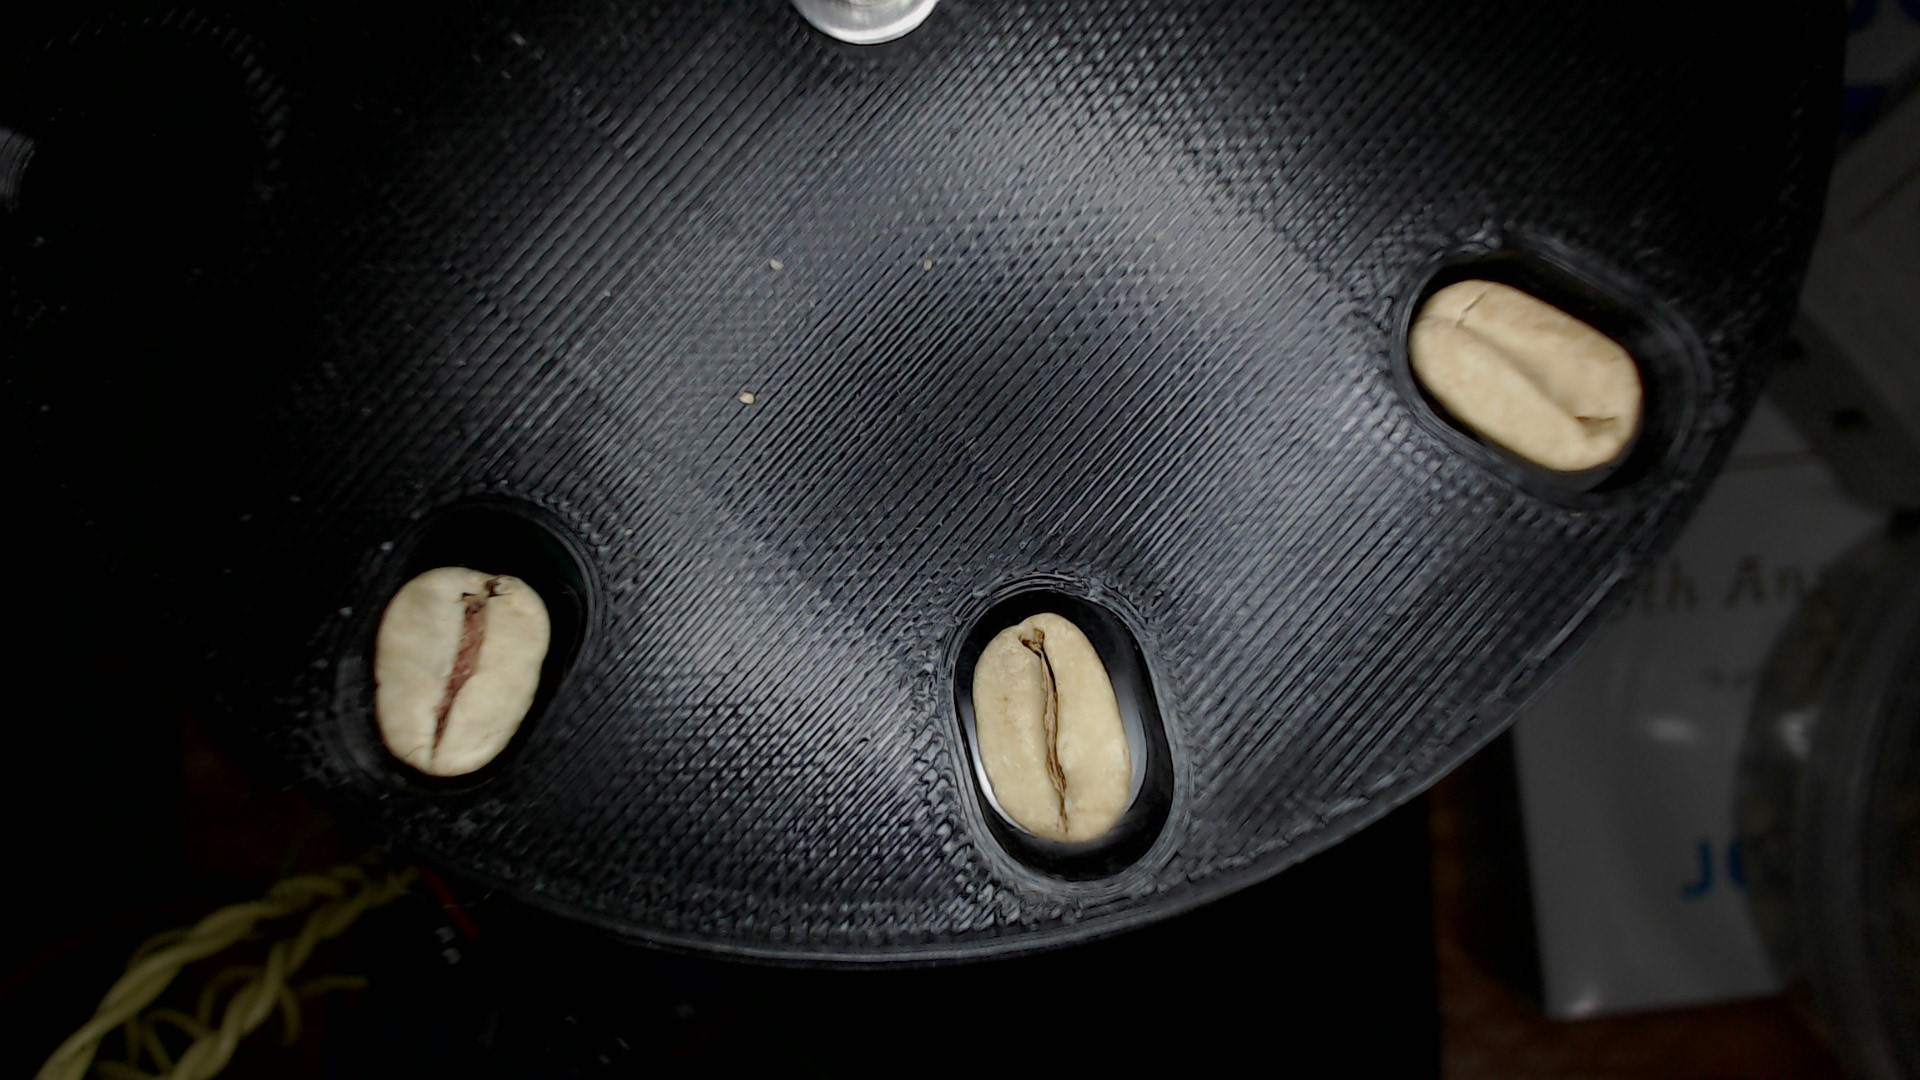
\includegraphics[width=0.3\textwidth]{ch5/2nd-Iteration-Table/Floater.jpg} \\
		\textbf{Dried Cherry}  & \textbf{Floater} \\[6pt]
	\end{tabular}
	\begin{tabular}{cc}
		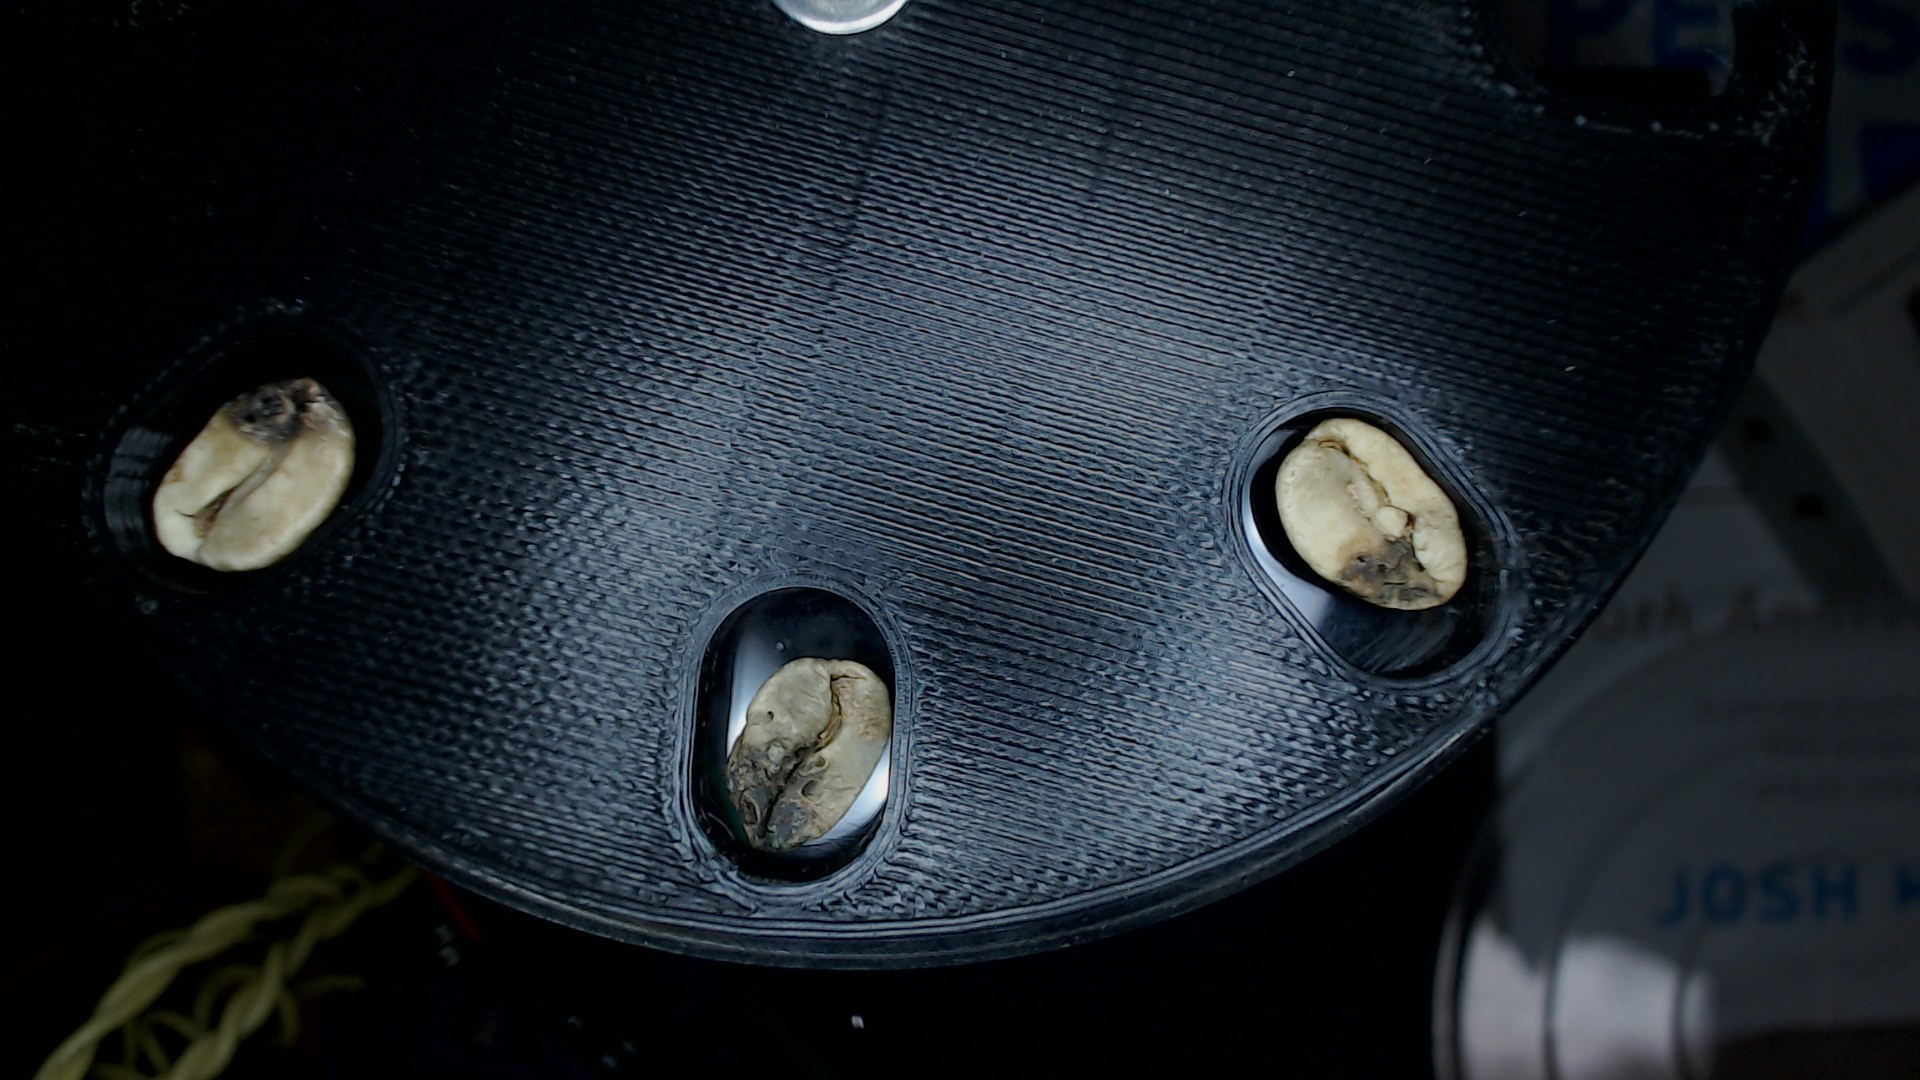
\includegraphics[width=0.3\textwidth]{ch5/2nd-Iteration-Table/FungusDamage.jpg} &
		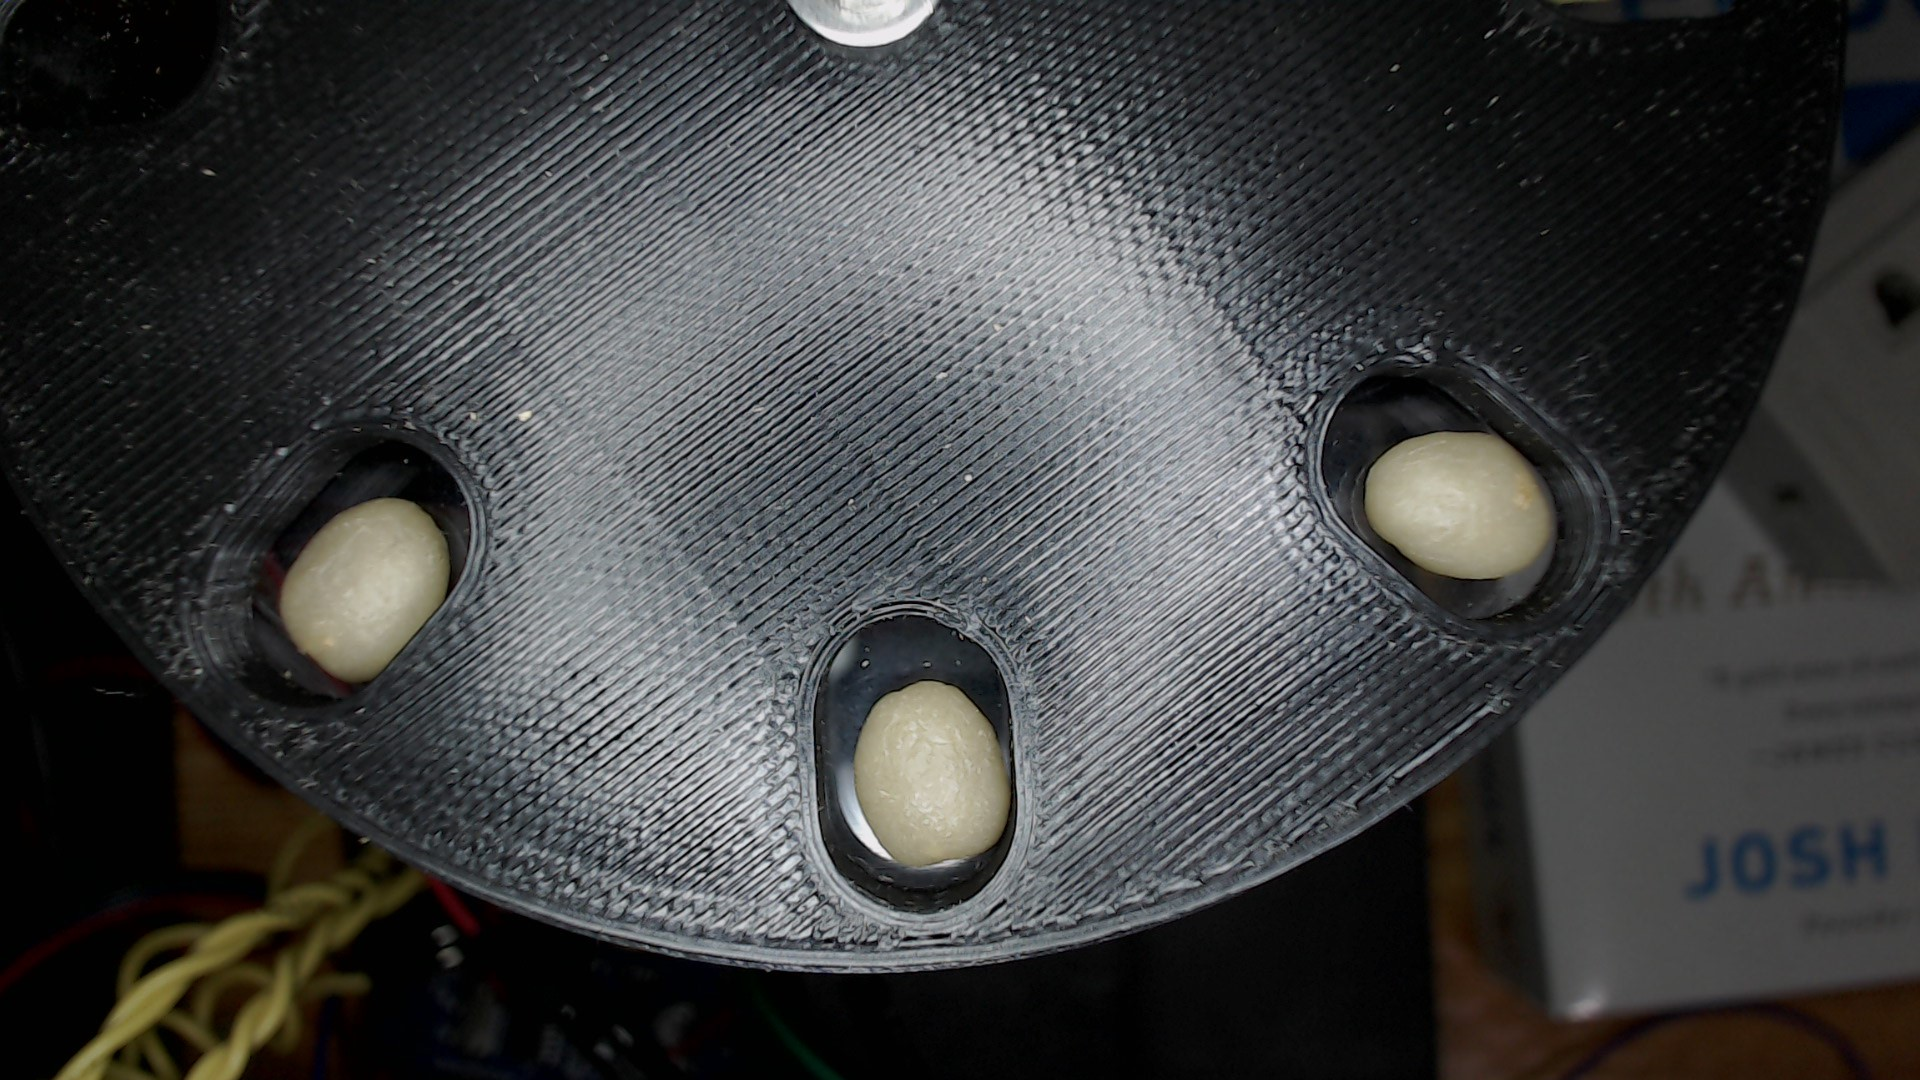
\includegraphics[width=0.3\textwidth]{ch5/2nd-Iteration-Table/Good.jpg} \\
		\textbf{Fungus Damage}  & \textbf{Good} \\[6pt]
	\end{tabular}
	\begin{tabular}{cc}
		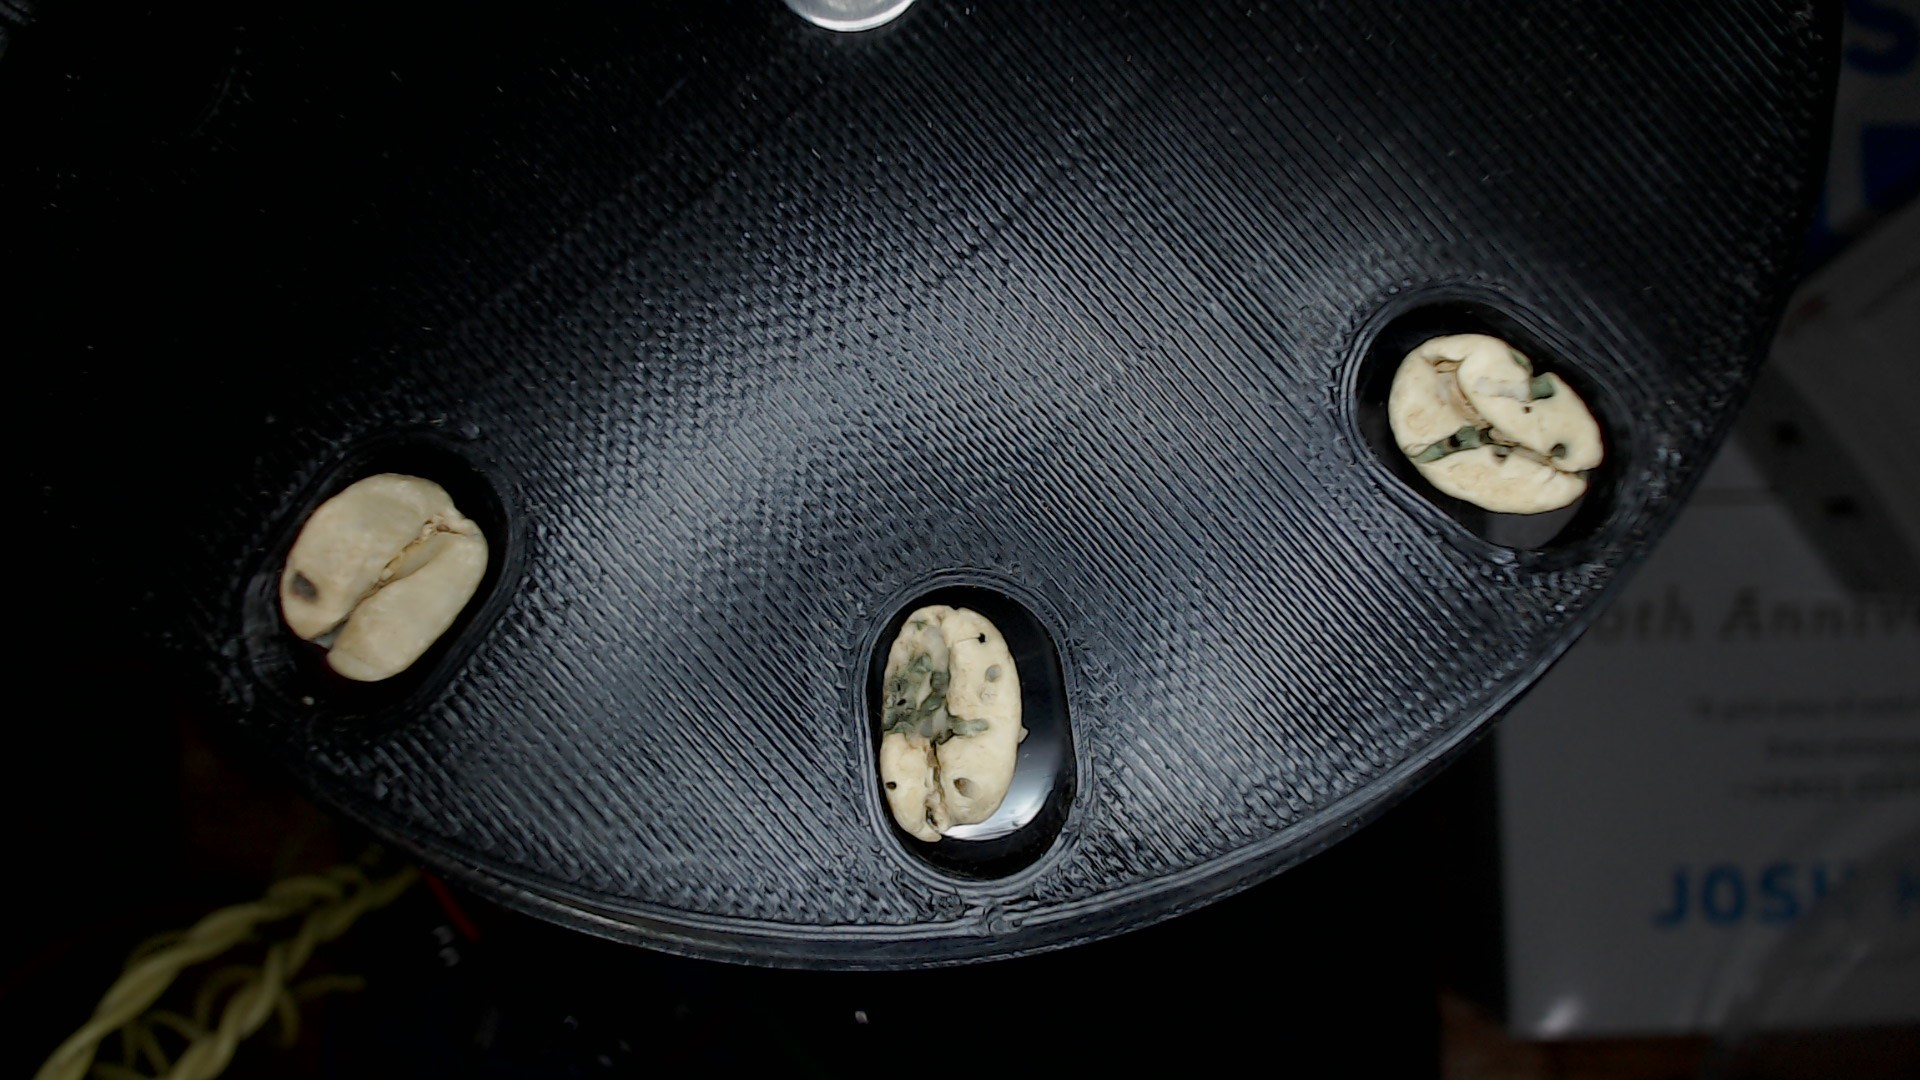
\includegraphics[width=0.3\textwidth]{ch5/2nd-Iteration-Table/InsectDamage.jpg} &
		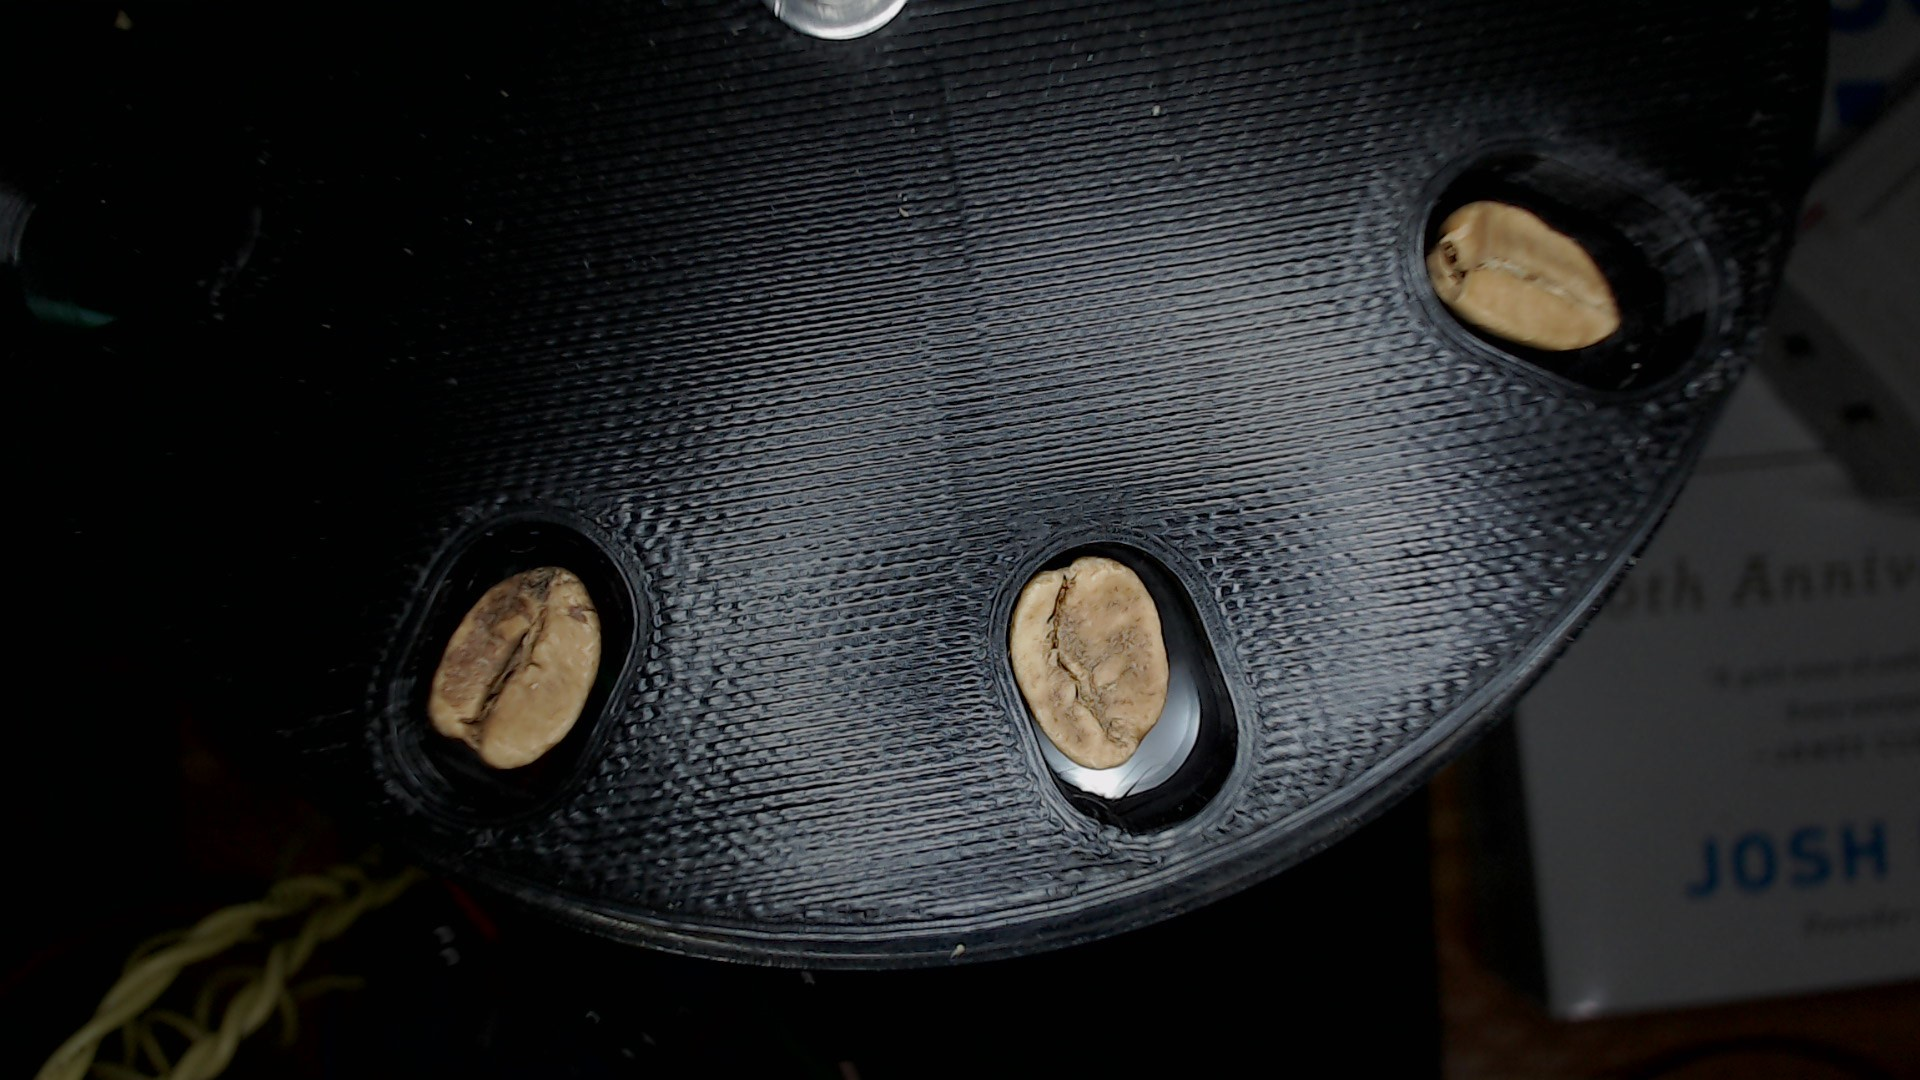
\includegraphics[width=0.3\textwidth]{ch5/2nd-Iteration-Table/Sour.jpg} \\
		\textbf{Insect Damage}  & \textbf{Sour} \\[6pt]
	\end{tabular}
	\caption{Sample Images from the Second Iteration of Dataset Collection}
\end{figure}

The second iteration focused on real-world implementation, using the system's built-in webcam to capture images directly from the inspection tray. This setup represents the ideal condition, as it replicates the actual environment where the model will operate. The images captured in this iteration directly reflect what the system will process in a practical application, allowing for better generalization and real-time adaptability.

\section{Dataset Preprocessing}
\label{sec:dataset_prep}
\subsection{Dataset Splitting}

The dataset is divided into train, validation, and test sets in a 70-20-10 ratio. The training dataset will be used for model learning, which allows it to identify patterns in the image. The validation set is used to assess the model’s performance and fine-tune the parameters of the model during training. This is an iterative process wherein the model learns from the training data and is then evaluated on and fine-tuned on the validation dataset. Finally, the test set is used for evaluating the model’s final performance, assessing its ability to generalize to new data.

\subsection{Image Annotation}

Roboflow Annotate was used to label images of coffee beans. The platform was used for two separate datasets: one for the detection model, the other for the classification model. In the detection dataset, bounding boxes were drawn around individual coffee beans and labeled accordingly. For the classification dataset, the trained detection model was used to crop individual coffee beans from the raw dataset, which were the categorized into the eight different classifications. Roboflow was chosen for its ability to store datasets in the cloud and its support for different annotation formats, such as COCO and YOLO, ensuring compatibility with different deep learning models during experimentation.

\subsection{Dataset Augmentation Techniques}

Data augmentation techniques were applied using Roboflow’s tools to improve the model generalization. Different augmentations such as rotation, flipping, blur, brightness and contrast adjustment, and noise were used to simulate variations, which helps prevent overfitting and improve the model’s ability to identify defects in different lighting conditions and orientations.

\section{Density Analysis}
\label{sec:density_analysis}

\subsection{Density Estimation}
To estimate the volume of the bean through computer vision, bounding boxes are implemented to first determine the area to be used for the volume estimation. Using the bounding boxes to determine a pixel value for the green coffee bean, this will be used to scale the image gathered from pixels to their estimated length and width. 

Through the estimated length and width gathered, this is compared to the actual length and width of the green coffee bean to compare both parameters. Through this, it is possible to estimate the volume of the green coffee bean through computer vision. The formula for triaxial ellipsoid is used to determine the volume of the green coffee bean.

The total volume of the batch of beans was measured by the water displacement technique, a commonly used method to measure the volume of solids that are irregularly shaped. The beans were fully immersed in a water-filled graduated cylinder, and the rise in water level was measured. The volume of water displaced is equivalent to the combined volume of the batch of beans, measured in cubic centimeters (cm$^3$).

Comparing the volume measured through water displacement and the volume gathered by computing for the volume using the triaxial ellipsoid volume formula, the volumes differ by -6.52\% up to +6.67\%, with most errors within the $\pm$5\%. This indicates that the model used to determine the volume of the green coffee bean is consistent with the ground-truth measurements. 


The overall weight of the beans was determined by a high-precision digital scale (at least to 0.001 g resolution). Both the mass and volume are known, and the batch density may be calculated through the use of the standard formula for density:

\[
\text{Batch Density} = \frac{\text{Total Mass of Beans} \, (g)}{\text{Total Volume Displaced} \, (cm^3)}
\]

Obtaining the volume through computer vision, and obtaining the weight of the bean through the precision scale, an estimated density is obtained that will be used to sort out the less dense from th dense beans. 

\subsection{Density Threshold Calibration}
\label{sec:density_threshold_calibration}
Setting the threshold for bean density is crucial for the stage 2 sorting of the system, which involves measuring the density of each bean. In order to set a threshold for density-based classification, a calibration batch of Good quality coffee beans was chosen. The beans were confirmed to be free of defects and representative of typical specialty-grade coffee by the farmer. The threshold density was calculated by determining the average density of this batch through direct measurements of mass and volume.

The computed average density served as the threshold value in the system. During automated classification, individual bean density is calculated using estimated volume (from image analysis) and actual weight (from the precision scale via RS232 communication). Beans with a density lower than the threshold are classified as less dense, while those meeting or exceeding the threshold are considered dense, indicating higher quality.

\section{Model Training}

\subsection{Image Detection Models}

The object detection model identifies and isolates the coffee beans from the background. For this task, different models were explored:

\begin{enumerate}
	\item \textbf{RF-DETR}
	 
	A transformer-based object detection model that eliminates the need for anchor boxes, improving small object detection.

	\item \textbf{YOLOv11}
	
	A CNN-based YOLO variant that incorporates the C3k2 block, SPPF, and C2PSA components to enhance feature extraction and detection accuracy.

	\item \textbf{YOLOv12}
	
	The latest YOLO version and attention-centric model that integrates transformer-based components to enhance performance while maintaining real-time efficiency.
\end{enumerate}

\subsection{Image Classification Models}
Following detection, each identified coffee bean was cropped and classified based on its defect type. The classification models used included:

\begin{enumerate}
	\item \textbf{EfficientNetV2}
	 
	A convolutional neural network (CNN) designed for high efficiency and accuracy, balancing computational cost and performance.
	
	\item \textbf{YOLOv8}
	
	A lightweight yet highly accurate model that supports both object detection and classification, making it suitable for real-time applications.

	\item \textbf{YOLOv11}
	
	A classification-specific adaptation of YOLOv11, leveraging enhanced feature extraction techniques for defect recognition.
	
	\item \textbf{YOLOv12}
	
	A classification variant of YOLOv12, incorporating advanced attention mechanisms to improve accuracy.

	\item \textbf{Vision Transformer (ViT)}

	The Vision Transformer (ViT) processes images as sequences of tokens for classification \cite{Dosovitskiy_Beyer_Kolesnikov_Weissenborn_Zhai_Unterthiner_Dehghani_Minderer_Heigold_Gelly_2021}. A learnable “class token” is added to the sequence to support classification. Through the attention mechanism, it captures dependencies between image tokens. The encoder is composed of repeated multi-head self-attention and feedforward layers, with self-attention computing weighted sums of sequence elements.
\end{enumerate}

\subsection{Bean Classification Logic}
To ensure proper classification, conditions are set based on how the top and bottom-side of the beans are categorized. For a bean to be labeled Good, both sides need to be classified as such. Similarly, Dried Cherry requires both sides to be classified as such, since Black beans can resemble Dried Cherry on its outer side. Moreover, both sides must be classified as Fungus Damage to be considered as such. If one side is classified as Black and the other Dried Cherry, or both are Black, then it will be labeled as Black.  The rest of the defect types are sufficient for single-side detection, as seen in Table \ref{tab:pseudocode_classification}.


\begin{table}[H]
	\caption{Classification Algorithm for Coffee Beans}
	\label{tab:pseudocode_classification}
	{\footnotesize
	\begin{tabular}{lll}
	\hline
	\hline
	{\bfseries Input(s):} & & \\
	$top\_class$ & : & classification result from top camera; $top\_class \in \mathbb{Z}^{+}$ \\
	$bottom\_class$ & : & classification result from bottom camera; $bottom\_class \in \mathbb{Z}^{+}$ \\
	\hline
	{\bfseries Output(s):} & & \\
	$class$ & : & final bean classification (Good, Defective, or specific defect) \\
	\hline
	\hline
	\\
	\end{tabular}
	}
	\begin{algorithmic}[1]
	{\footnotesize
		\IF{$top\_class = 5 \wedge bottom\_class = 5$}
			\STATE $class \Leftarrow$ ``Good''
		\ELSIF{$top\_class = 2 \wedge bottom\_class = 2$}
			\STATE $class \Leftarrow$ ``Dried Cherry''
		\ELSIF{$(top\_class = 0 \wedge bottom\_class = 0) \vee (top\_class = 0 \wedge bottom\_class = 2) \vee (top\_class = 2 \wedge bottom\_class = 0)$}
			\STATE $class \Leftarrow$ ``Black''
		\ELSIF{$top\_class = 4 \wedge bottom\_class = 4$}
			\STATE $class \Leftarrow$ ``Fungus Damage''
		\ELSIF{$top\_class = 6 \wedge bottom\_class = 6$}
			\STATE $class \Leftarrow$ ``Insect Damage''
		\ELSIF{$top\_class = 1 \vee bottom\_class = 1$}
			\STATE $class \Leftarrow$ ``Broken''
		\ELSIF{$top\_class = 7 \vee bottom\_class = 7$}
			\STATE $class \Leftarrow$ ``Sour''
		\ELSIF{$top\_class = 3 \vee bottom\_class = 3$}
			\STATE $class \Leftarrow$ ``Floater''
		\ELSE
			\STATE $class \Leftarrow$ ``Defective''
		\ENDIF
		\RETURN $class$
	}	
	\end{algorithmic}
\end{table}


\subsection{Model Evaluation}
Each trained model will be tested on the system, with a predetermined set of beans. The results from this test are analyzed by using a confusion matrix, providing a detailed breakdown of the model’s performance for each category. The confusion matrix provides a way to interpret classification results by defining the following parameters:
\begin{itemize}
    \item \textbf{True Positives (TP)} - The number of correctly classified instances for a specific defect type.
    \item \textbf{False Positives (FP)} - The number of times a different category was incorrectly classified as this defect type.
    \item \textbf{True Negatives (TN)} - All correctly classified instances excluding the defect category in question.
    \item \textbf{False Negatives (FN)} - The number of times this defect type was classified as something else.
\end{itemize}

Through these parameters, key performance metrics such as accuracy, precision, recall, and F1-score were computed to evaluate the system’s performance in different classifications as shown below. This test will assist in determining what types of defects the system correctly classifies and which types might need improvements in image preprocessing, dataset expansion, or optimization of the machine learning model. The outcome will be applied to optimize the sorting algorithm for minimal misclassifications to ensure greater reliability in real-world defect detection.

\begin{enumerate}
	\item \textbf{Accuracy} measures overall correctness of the classification model
	\begin{equation}
	Accuracy = \frac{TP + TN}{TP + TN + FP + FN}
	\end{equation}

	\item \textbf{Precision} measures how many of the predicted positive classifications were actually correct
	\begin{equation}
	Precision = \frac{TP}{TP + FP}
	\end{equation}

	\item \textbf{Recall} evaluates how well the model identifies actual positive cases
	\begin{equation}
	Recall = \frac{TP}{TP + FN}
\end{equation}
	
	\item \textbf{F1-score} represents the harmonic mean of precision and recall
\begin{equation}
	F1\text{-}Score = 2 \times \frac{Precision \times Recall}{Precision + Recall}
	\end{equation}
\end{enumerate}

\subsection{Model Benchmarking and Selection}
A total of 5 models were trained and tested within the actual system to determine the most effective one. These models trained and evaluated include EfficientNetV2, YOLOv8, YOLOv11, YOLOv12, and ViT. Each model was assessed using the defined performance metrics and compared accordingly. The model with the highest overall performance will be selected for deployment in the system.


\section{Hardware Development}
The hardware elements of the system, two-stage automated coffee bean sorter, are developed to provide effective and precise sorting using a mix of mechanical and electronic components. Each element is designed and tested to maximize the sorting process while providing system reliability.

\subsection{Screw Feeder}
\begin{figure}[H]
    \centering
    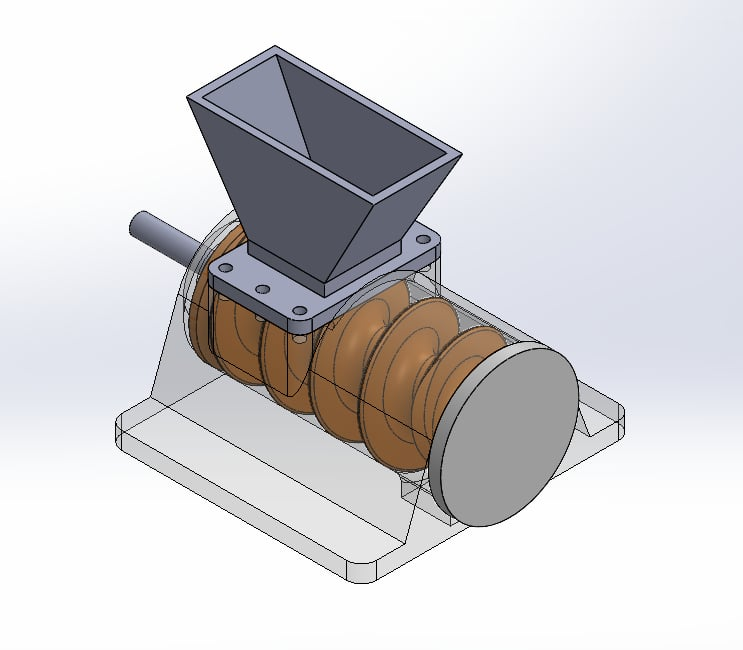
\includegraphics[width=9cm]{ch5/Screw_Feeder_Design.jpg}
    \caption{Screw Feeder 3D Design}
    \label{fig:screw_feeder}
\end{figure}
Screw feeder is the most essential of the devices as it governs the beans of coffee moving into the system. It operates mostly to deliver the beans consistently in terms of volume and ensures they do not bundle up and fall into the system in heavy masses, causing beans build up on the rotating conveyor table. The feeder is driven by a 12V DC motor, and the rotation speed is regulated using PWM. Through a constant and controlled flow, the screw feeder avoids clogging and provides a consistent input into the inspection tray, enhancing overall system performance. Figure \ref{fig:screw_feeder} shows the actual 3D model design of the screw feeder used in the system. 

\subsection{Rotating Conveyor Table}
\begin{figure}[H]
    \centering
    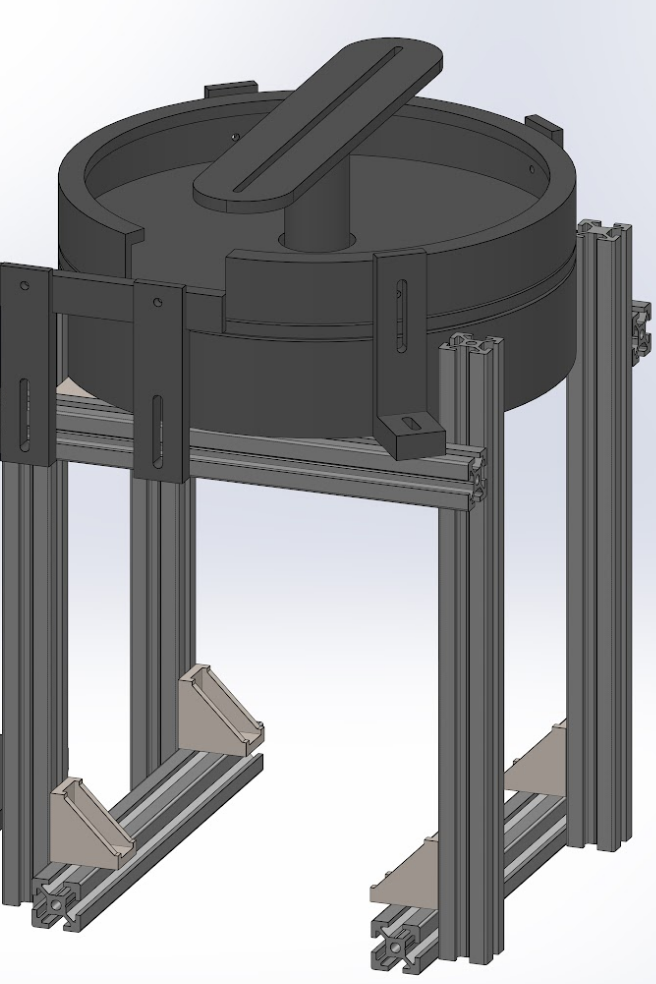
\includegraphics[width=7cm]{ch5/Rotating_Conveyor_Table_Design.png}
    \caption{Rotating Conveyor Table 3D Design}
    \label{fig:rotating_conveyor}
\end{figure}
The conveyor table, as shown in Figure \ref{fig:rotating_conveyor}, rotates to move the coffee beans from the feeding mechanism to the inspection tray. The table contains aluminum guides to linearly arrange the beans prior to dropping on the inspection tray. The conveyor is powered by a 12V DC motor, which offers consistent movement and regulated speed to avoid misalignment. By incorporating a turning mechanism, the conveyor guarantees beans are well oriented prior to inspection tray entry, minimizing classification errors due to faulty positioning.

\begin{figure}[H]
    \centering
    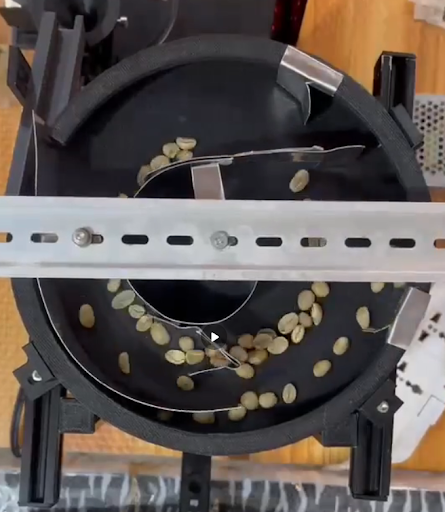
\includegraphics[width=9cm]{ch5/Rotating_Conveyor_Table_with_Aluminum_Guides.png}
    \caption{Rotating Conveyor Table with Aluminum Guides}
    \label{fig:rotating_conveyor_aluminum}
\end{figure}
As shown in Figure \ref{fig:rotating_conveyor_aluminum}, there are aluminum guides on the rotating conveyor table that ensures coffee beans to be linearly arranged. This linear arrangement of beans significantly helped the system to ensure that coffee beans are dropped onto the slide, which connects the conveyor table to the inspection try, in a one-by-one manner. In addition, the guides are also installed to keep the beans from accumulating in one area, which can cause the jamming of beans. The researchers tested the different motor speeds to observe the optimal settings that will not cause bean jamming and meet the minimum sorting speed of the system. However, while the aluminum guides are effective in arranging the beans linearly, it was hard to re-calibrate or adjust. Another problem was it was easy to be deformed whenever there was jamming of beans. Upon printing the model, the bearing of the rotating mechanism was also not robust enough to hold the motor in higher RPM. There are instances where the gearing mechanism between the motor and the conveyor table experiences jamming, resulting in the conveyor table temporarily ceasing rotation. This issue typically arises from misalignment or friction within the gear interface, which hinders the smooth transfer of torque from the motor to the conveyor table.


\begin{figure}[H]
    \centering
    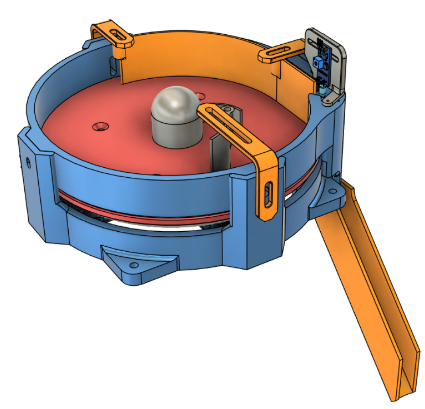
\includegraphics[width=9cm]{ch5/Revised_Rotating_Conveyor_Table.png}
    \caption{Revised Rotating Conveyor Table}
    \label{fig:revised_rotating_conveyor}
\end{figure}
Figure \ref{fig:revised_rotating_conveyor} shows the re-designed conveyor table. In this revision, calibration of the guides was easier since it can be moved by only loosening the screws. To avoid the issue caused by the misalignment within the gear of the previous rotating table mechanism, the researchers opted to revise the design. The new iteration of the rotating conveyor table was redesigned using a Lazy Susan bearing. In this modification, smoother rotation was observed. 

\begin{figure}[H]
    \centering
    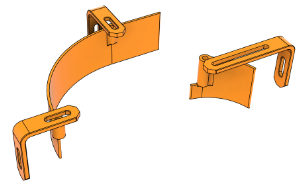
\includegraphics[width=9cm]{ch5/3D-Printed_Guides.png}
    \caption{3D Printed Guides}
    \label{fig:3d_printed_guides}
\end{figure}
In addition, the previously aluminum guides were replaced with 3D-printed guides that were screwed onto the table walls. The revised design allowed for easier calibration, as the guides could be repositioned simply by loosening the screws, enabling more precise alignment of beans. 

\begin{figure}[H]
    \centering
    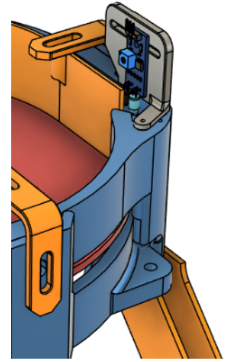
\includegraphics[width=5cm]{ch5/IR_Sensor_Placement.png}
    \caption{IR Sensor Placement}
    \label{fig:ir_sensor_placement}
\end{figure}
Another point of improvement was the placement of the IR sensor, which was redesigned to be adjustable. This adjustability allowed faster calibration and ensured accurate detection of beans at the table’s edge, further enhancing the system’s reliability and consistency. Initially, the rotating conveyor table is set at a fixed and slow speed to ensure that coffee beans are dropped into the inspection tray one-by-one. However, at this rate, the time travel time of the first bean dropped from the center of the table is very long. Thus, the group decided to add an IR sensor at the edge of the rotating table as seen in Figure X. The sensor’s responsibility is to detect if there is a bean at the edge. If there is no bean detected, the rotating table is set to a higher speed to expedite the process. On the other hand, if a bean is detected by the sensor, the rotation of the table is adjusted in such a way that it is able to drop the beans one-by-one onto the inspection tray. With this sensor integrated into the system, a higher speed can be set for the rotating table, minimizing the time travel of the beans from the center to the inspection tray, resulting in a faster sorting time for the first stage.

\subsection{Stage 1: Defect Sorting (Machine Vision and Inspection Tray)}

\begin{figure}[H]
    \centering
    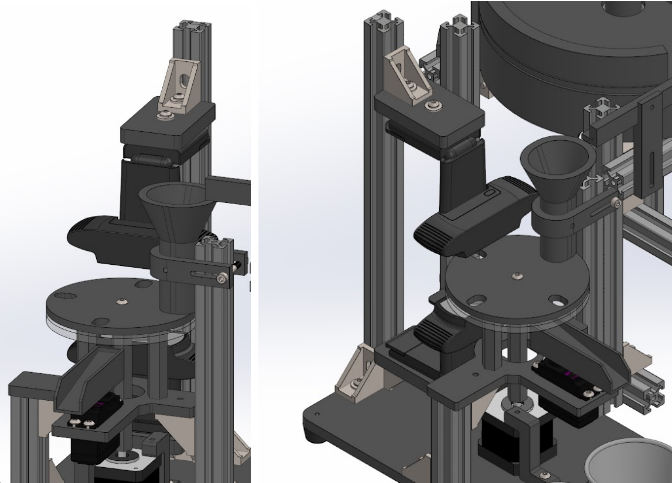
\includegraphics[width=12cm]{ch5/Inspection_Tray_Design.png}
    \caption{Inspection Tray 3D Design}
    \label{fig:inspection_tray_design}
\end{figure}

The inspection tray is the main component for the first-stage sorting mechanism. The inspection tray is used to support beans in a stable and constrained position for a short time, enabling the camera to take high-resolution images without motion blur. The NEMA 17 stepper motor drives the movement of the inspection tray, enabling accurate alignment with the vision system's image processing pipeline. The tray surface is created to reduce reflections and enhance contrast so that the camera can precisely detect defects like cracks, discoloration, or insect infestation. In addition, the surface is made of clear acrylic to allow a clear image for the camera positioned at the bottom of the tray. Lastly, a rotatable slider controlled by a 5V servo motor serves as the main segregator of the good beans from the defective beans. 

\subsection{Stage 2: Density Sorting (Precision Scale and Servo Mechanism)}
\label{sec:density_sorter}

% TODO: ADD FIGURE
\begin{figure}[H]
    \centering
    \includegraphics[width=12cm]{ch5/Density_Sorter_Mechanism_Design.png}
    \caption{Density Sorter Mechanism Design}
    \label{fig:density_sorter_design}
\end{figure}
The density sorter is the second-stage sorting system, tasked with sorting coffee beans according to their measured density. This is achieved by initially measuring each bean's mass using a precision weighing scale and volume using the computer vision. After calculating the density, the system triggers a sorting system powered by a geared 5V  servomotor, which sorts beans into various collection bins according to their classification. This sorting operation is such that high-density beans are kept separate from low-density beans. The density sorter's accuracy is verified by comparing the results of its classification to manual weighing measurements (ground truth data).

\begin{figure}[H]
    \centering
    \includegraphics[width=9cm]{ch5/Precision_Scale.png}
    \caption{Precision Scale}
    \label{fig:precision_scale}
\end{figure}
The U.S. Solid Electronic Precision Balance (0.01g, 1200g capacity, RS232 port, AC/DC power) was selected for the density sorting mechanism because it is highly accurate, transmits data in real-time, and is well-calibrated. Its 0.01g precision guarantees accurate mass readings, which are critical to precise density calculations in sorting coffee beans. The RS232 port facilitates smooth integration with the microcontroller for automatic data processing and sorting decisions, minimizing manual errors. Its dual power source (AC and battery) also guarantees uninterrupted operation in different environments, making it a dependable and efficient part of the coffee bean sorting system.

\section{Hardware and Software Integration}

\subsection{Serial Communication}
\label{sec:serial_communication}
\begin{figure}[H]
    \centering
    \includegraphics[width=12cm]{ch5/Serial_Communication_Flow_for_Stage_1_Classification.png}
    \caption{Serial Communication Flow for Stage 1 Classification}
    \label{fig:serial_comm_flow}
\end{figure}
The system is generally composed of hardware and software components. Hardware components are mainly responsible for collecting data from the coffee beans such as the camera and IR sensor, and the sorting mechanisms such as servo motors and stepper motors. On the other hand, the software components are the brain of the system which is mainly responsible for data processing such as image detection, defect classification of the beans, volume and density computation, and control of the mechanisms. Since the system has two major components, software and hardware, they should be integrated together for the system to be as effective. Thus, serial communication was utilized to integrate the hardware and software components of the system. Serial communication is a significant component in the system as it serves as the communication medium of the hardware and software. It enables real-time coordination between the software (YOLO-based image detection, classification, and density computation) and the hardware (running in Arduino microcontrollers). The said communication is established with the use of a USB serial interface using the pyserial library in Python. In addition, this is configured at a baud rate of 9600.

The system, specifically at the inspection tray mechanism where the YOLO detection and classification is implemented, has a function move\_stepper() responsible for sending the command from the Python code to the Arduino microcontroller. When the Arduino receive this command, it executes motor movement that allows the stepper motor to move at a certain angle that allows the camera to capture the bean. This function is crucial for the system as this is how each bean in the inspection tray is fed to the image processing side of the system. This movement rotates the mechanism holding the coffee beans, positioning the next bean beneath the top and bottom cameras for inspection. After the motor completes the movement, the Arduino will send back a message to the program running Python, signalling that the bean is ready for image capture and further processing. In addition, the Python script is continuously or constantly waiting for the Arduino’s message through the arduino.readline() function, ensuring seamless communication and faster processing. 


\subsection{Recommended Standard 232 (RS-232)}
\begin{figure}[H]
    \centering
    \includegraphics[width=12cm]{ch5/Precision_Scale_Integration_with_RS232.png}
    \caption{Precision Scale Integration with RS232 for Stage 2 Classification}
    \label{fig:rs232}
\end{figure}

The stage 2 classification is mainly composed of the sorting mechanism itself, and the precision scale to measure the mass of each bean. The bounding boxes from the stage 1 classification are used to estimate each bean’s volume. Additionally, the beans depth is also estimated through the IR sensor placed in the rotating conveyor table. With these measurements, the volume of each bean, the volume can be calculated using the Tri-axial Ellipsoid’s volume formula. 

The stage 2 classification, density-based sorting, is implemented using a combination of RS232 and USB serial communication. In this stage, each bean that has been classified as ‘Good’ from stage 1 is again sorted based on the density. The RS232’s main responsibility is to simultaneously record and pass the values to the Arduino Nano to compute the density. Subsequently, the data from the computations are the deciding factor whether to sort out the bean or not, depending on the predefined threshold for the system. 

\section{Prototype Setup}
\subsection{Actual Setup}

\begin{figure}[H]
    \centering
    \includegraphics[width=9cm]{ch5/Actual_Setup_of_the_System.jpg}
    \caption{Actual System Setup (1st Iteration)}
    \label{fig:actual_setup_v1}
\end{figure}

\begin{figure}[H]
    \centering
    \includegraphics[width=9cm]{ch5/Actual_Setup_of_the_System_2.png}
    \caption{Actual System Setup (2nd Iteration)}
    \label{fig:actual_setup_v2}
\end{figure}

Physical integration of the automatic coffee bean sorter system comprises various integrated parts with the purpose of enabling effective, accurate, and methodical sorting in terms of visual defects as well as density categorization. The system involves integration of mechanical, electronic, and computer vision technologies for optimizing sorting. To begin the process, coffee beans are added to a revolving conveyor table, which is the main mechanism of transport used for feeding the beans into the inspection system. The conveyor features aluminum guides positioned strategically along it to ensure linear alignment of the beans as they travel. Linear alignment is required to avoid overlap and misclassification, since individual processing by the machine vision system is necessary for each bean.Once the beans travel further along the conveyor, they are conveyed onto the inspection tray. There, they are viewed in multiple perspectives by two high-definition cameras. A two-camera imaging process ensures improved defect detection by providing a full, thorough evaluation of the surface, shape, and texture of the bean. The images are then processed with a deep learning-based classification algorithm that classifies each bean as either defective or good according to predefined defect types like black beans, dried cherries, fungus damage, insect damage, sour beans, floaters, and broken beans. After classification, the system triggers the defect sorting mechanism, which physically takes out defective beans from the processing line. The mechanism includes a servo motor-powered sorting slide, which diverts defective beans into a distinct collection bin. Good beans that are classified are taken to the second level of sorting, which is density-based classification. At the density-based sorting level, good beans are weighed individually with a high-precision electronic balance. The U.S. Solid Electronic Precision Balance (0.01g, RS232) is embedded within the system to accurately weigh the mass of each bean. According to the calculation of density, beans are automatically sorted into corresponding collection bins using a second sorting mechanism regulated by a NEMA 17 stepper motor.

\subsection{Lighting Setup for Inspection Tray}

Lighting has a key importance in the image-based detection and classification system, specifically for the inspection tray. For the model to be more accurate and precise in classifying good and defective beans, correct lighting is important such that details like surface texture, color difference, and defects are properly rendered by the imaging system. Asymmetrical, unsteady, or low-quality lighting can create shadows, reflections, or overexposure, all of which lower the quality of input images and thus decrease the accuracy of object detection and classification models like YOLO. To improve the consistency and definition of images taken during inspection, the lighting arrangement above the inspection tray was refined incrementally throughout development. The refinements were intended to maximize the illumination conditions for both the top and bottom camera modules.


\begin{figure}[H]
    \centering
    \includegraphics[width=9cm]{ch5/Initial_Lighting_Setup.jpg}
    \caption{First Iteration of Lighting Setup}
    \label{fig:first_lighting}
\end{figure}

Figure \ref{fig:first_lighting} shows the initial lighting setup that the researchers implemented on the system. The initial lighting arrangement was based on a single top-mounted LED lighting. Although the arrangement was more than bright enough for the top camera, it introduced random shadows and highlights onto the bottom camera. As a result, only one side of the bean is accurately inspected. These random elements impacted the model's performance in detecting bean contours and separating surface flaws, particularly for dark beans or reflective-surface beans.


\begin{figure}[H]
    \centering
    \includegraphics[width=9cm]{ch5/Modified_Lighting_Setup.png}
    \caption{Second Iteration of Lighting Setup}
    \label{fig:second_lighting}
\end{figure}

For the second iteration of the lighting setup, the researchers decided to add another LED strip lighting at the side of the inspection tray, while keeping the LED lighting mounted at the top. This provided good lighting for both top and bottom cameras. However, the view of the bottom camera is still a bit dark.


\begin{figure}[H]
    \centering
    \includegraphics[width=9cm]{ch5/Final_Lighting_Setup.png}
    \caption{Final Iteration of Lighting Setup}
    \label{fig:final_lighting}
\end{figure}

To ensure that both camera views have sufficient lighting and avoid shadows, the researchers decided to use a total of three LED lights. One is a small ring light placed exactly above the inspection tray. Another LED light is a strip light placed at the side of the inspection tray to improve lighting at the side of each bean. Another small LED light is placed under the inspection tray to ensure that the bottom camera has enough lighting. Electrical tape was applied to the side of the acrylic plate to block excess lighting, thereby optimizing the lighting setup of the system.

\begin{figure}[H]
    \centering
    \includegraphics[width=9cm]{ch5/Top_and_Bottom_View_of_the_Cameras.png}
    \caption{Top and Bottom View of the Cameras}
    \label{fig:top_and_bottom}
\end{figure}

\subsection{System Operation}

The system operation follows a sequential process to ensure the effective sorting of green coffee beans (GCBs) based on its classification and density. The automated system consists of two primary stages: 1st Stage which is the machine vision-based classification and 2nd stage which is the density-based sorting.

The process beings in the inputting of unsorted GCBs (Contains good and defective beans) into the screw feeder, which regulates the controlled and consistent delivery of the beans into the rotary conveyor table. The conveyor table is designed with aluminum guides to ensure a linearized formation of the beans to mitigate jamming. This also ensures a controlled movement of beans, ensuring that they drop onto the inspection tray one at a time. As the bean goes towards the edge of the conveyor table, the IR sensors detects the beans and stops the rotation to ensure the one-by-one inspection of the beans, this also prevents clogging, and jamming once the beans are dropped into the inspection tray. 

The first phase involves machine-vision classification. Once the GCBs reach the inspection tray, each bean is analyzed one-by-one using a machine vision system consisting of top and bottom cameras. The system captures high-resolution images of the bean and processes the data to determine which classification it belongs. If the bean is identified as defective, a signal is sent to the servo motor, which redirects the bean into the defective bin for disposal, if the bean is classified as good, it then proceeds to the second phase of the system

The second stage involves density-based sorting, where each GCB's weight is measured using a precision scale, while its volume is determined by the bounding boxes from the first stage. These bounding boxes were used to estimate the dimensions of the beans and used the Ellipsoid volume formula for volume estimation.  

The sorting mechanism activates, directing beans into designated collection bins based on their density. High-density beans, often associated with specialty-grade quality, are separated from low-density, commercial-grade, or defective beans. 

\section{Prototype Testing}

\subsection{Sorting Speed}

\begin{figure}[H]
	\centering
	\begin{tabularx}{\textwidth}{p{0.3\textwidth}|p{0.2\textwidth}|p{0.2\textwidth}|p{0.2\textwidth}}
		\caption{Sorting Speed Testing Table} \label{tab:sorting_speed} \\
		\hline \hline
		\textbf{Test Condition} & \textbf{Conveyor Table Speed (RPM)} & \textbf{Inspection Tray Speed (RPM)} & \textbf{Sorting Speed (Beans per Minute)} \\
		\hline
		100\% Good Beans &  &  &  \\
		\hline
		75\% Good, 25\% Defective Beans &  &  &  \\
		\hline
		50\% Good, 50\% Defective Beans &  &  &  \\
		\hline
		25\% Good, 75\% Defective Beans &  &  &  \\
		\hline
		100\% Defective Beans &  &  &  \\
		\hline
	\end{tabularx}
\end{figure}

The sorting speed of the system will be determined by conducting at least five trials. Each trial will be exactly conducted for one minute. The number of beans sorted out within the time frame are considered as the sorting speed in beans per minute. Then, the average sorting speed from the five trials is computed. In each trial session, controlled variables such as motor speed of the inspection tray and rotating conveyor table are varied to observe the optimal setting for the system, ensuring that there are no beans jamming in the tray and fast enough to meet the minimum sorting speed. Table \ref{tab:sorting_speed} shows the different conditions for each trial to ensure that the sorting speed across different type of beans are considered. 

\subsection{Defect Sorting Accuracy}

To measure the system’s performance on defect sorting, two separate tests were performed. The first test was performed to measure the system’s accuracy on classifying the seven defect types including good beans. On the other hand, a second test was conducted to measure the system’s reliability on sorting out defective beans from good beans. In this test, there are only two classifications – defective beans and good beans. 

\begin{figure}[H]
	\centering
	\begin{tabular}{cc}
		\includegraphics[height=0.2\textwidth]{ch5/Per-Classification Test Dataset/Black.png} &
		\includegraphics[height=0.2\textwidth]{ch5/Per-Classification Test Dataset/Broken.png} \\
		\textbf{Black - 30 Beans}  & \textbf{Broken - 30 Beans} \\[6pt]
	\end{tabular}
	\begin{tabular}{cc}
		\includegraphics[height=0.2\textwidth]{ch5/Per-Classification Test Dataset/Dried Cherry.png} &
		\includegraphics[height=0.2\textwidth]{ch5/Per-Classification Test Dataset/Floater.png} \\
		\textbf{Dried Cherry - 30 Beans}  & \textbf{Floater - 30 Beans} \\[6pt]
	\end{tabular}
	\begin{tabular}{cc}
		\includegraphics[height=0.2\textwidth]{ch5/Per-Classification Test Dataset/Fungus.png} &
		\includegraphics[height=0.2\textwidth]{ch5/Per-Classification Test Dataset/Good.png} \\
		\textbf{Fungus Damage - 30 Beans}  & \textbf{Good - 150 Beans} \\[6pt]
	\end{tabular}
	\begin{tabular}{cc}
		\includegraphics[height=0.2\textwidth]{ch5/Per-Classification Test Dataset/Insect.png} &
		\includegraphics[height=0.2\textwidth]{ch5/Per-Classification Test Dataset/Sour.png} \\
		\textbf{Insect Damage - 30 Beans}  & \textbf{Sour - 30 Beans} \\[6pt]
	\end{tabular}
	\caption{Per-Classification	Test Dataset}
	\label{fig:per_classification_test_dataset}
\end{figure}

Table \ref{fig:per_classification_test_dataset} shows the actual test dataset used in the first test. This test was conducted using the top two performing models after training. Based on the 70-20-10 training, validation, test split, the researchers gathered 30 beans for each defect type, and 150 for good beans. The test consists of 5 trials with the same test set. Each trial was divided into 8 parts, corresponding to each classification. In this test, if one of the cameras detects the specific defect type being tested, it is considered as correctly classified. However, for good beans, both cameras should be able to classify it as good to be considered as a correct classification.

\begin{figure}[H]
	\centering
	\begin{tabular}{cc}
		\includegraphics[height=0.2\textwidth]{ch5/Good vs. Defect Test Dataset/100-Good.png} &
		\includegraphics[height=0.2\textwidth]{ch5/Good vs. Defect Test Dataset/75Good-25Defect.png} \\
		\textbf{100\% Good}  & \textbf{75\% Good, 25\% Defects} \\[6pt]
	\end{tabular}
	\begin{tabular}{cc}
		\includegraphics[height=0.2\textwidth]{ch5/Good vs. Defect Test Dataset/50Goodt-50Defect.png} &
		\includegraphics[height=0.2\textwidth]{ch5/Good vs. Defect Test Dataset/25Good-75Defect.png} \\
		\textbf{50\% Good, 50\% Defects}  & \textbf{25\% Good, 75\% Defects} \\[6pt]
	\end{tabular}
	\begin{tabular}{cc}
		\includegraphics[height=0.2\textwidth]{ch5/Good vs. Defect Test Dataset/100-Defect.png} &
		\\
		\textbf{100\% Defects} & \\[6pt]
	\end{tabular}
	\caption{Good vs. Defective Test Dataset}
	\label{fig:good_vs_defective_test_dataset}
\end{figure}

The defect sorting accuracy by feeding 100 beans on each trial. For testing its accuracy for detecting good beans and defective beans, five trials are conducted containing 100 beans of good beans for the first trial, 75 good and 25 defects for the second trial, 50 good and 50 defects for the third trial, 25 good and 75 defects for the fourth trial, and 100 defects for the last trial. With these, the number of correctly classified and misclassified beans are logged into the system to compute for accuracy. 

\begin{figure}[H]
	\centering
	\begin{tabularx}{\textwidth}{p{0.3\textwidth}|p{0.2\textwidth}}
		\caption{Dataset Distribution for Overall Testing} \label{tab:dataset_distribution} \\
		\hline \hline
		\textbf{Bean Classification} & \textbf{Bean Count} \\
		\hline
		Good & 150 \\
		\hline
		Black &  30 \\
		\hline
		Broken & 30 \\
		\hline
		Dried Cherry & 30 \\
		\hline
		Floater & 30 \\
		\hline
		Fungus Damage & 30 \\
		\hline
		Insect Damage & 30 \\
		\hline
		Sour & 30 \\
		\hline
		\textbf{Total Beans} & \textbf{360} \\
		\hline
	\end{tabularx}
\end{figure}

Lastly, to assess the overall accuracy and reliability of the first stage, machine vision-based defect classification,  a trial consisting of a predefined dataset of 360 coffee beans was conducted. The good classification consists of 150 beans, while each defect, such as black, dried cherry, fungus, insect damage, sour, floater, and broken beans, consists of 30 beans as shown in Table \ref{tab:dataset_distribution}.

\subsection{Density Sorting Accuracy}

To assess the accuracy of the mechanism, it will rely on measuring the accuracy and the reliability of the density sorting mechanism in sorting out the dense beans to the less dense beans. To successfully determine the accuracy of the system, the basis will be the scale, where the system should be able to sort the dense beans to the less dense bean in relation to the detected weight in the scale. A successful system should be able to sort with an accuracy of 85\%.

	%\stopcontents[chapters]
	\cleardoublepage
	
	%%%%%%%%%%%%%%%%%%%%%%%%%%%%%%%%%%%%%%%%%%%%%%%%
	\ifResultDiscuss 
	\chapter{Results and Discussions} 
	%	\label{ch:result_discuss} 
	%	\startcontents[chapters]
	%	\begin{SingleSpace}	
	%		\Mprintcontents 
	%	\end{SingleSpace}
		\begin{center}
	{\scriptsize
		\begin{tabularx}{\textwidth}{p{0.2\textwidth}|p{0.6\textwidth}|p{0.1\textwidth}}
			\caption{Summary of results for achieving the objectives} \label{tab:outcomes_per_objective} \\
			\hline 
			\hline 
			\textbf{Objectives} & 
			\textbf{Results} &
			\textbf{Locations}\\ 
			\hline 
			\endfirsthead
			\multicolumn{3}{c}%
			{\textit{Continued from previous page}} \\
			\hline
			\hline 
			\textbf{Objectives} & 
			\textbf{Results} &
			\textbf{Locations}\\ 
			\hline 
			\endhead
			\hline 
			\multicolumn{3}{r}{\textit{Continued on next page}} \\ 
			\endfoot
			\hline 
			\endlastfoot
			\hline
			
			
			\Paste{GO} & 

			\begin{itemize}
				\item Achieved to gather and create a unique dataset consisting of 500 good and 200 defective beans
				\item Achieved improvisation of the synchronization between the machine vision and embedded system.
			\end{itemize}
			
			& Sec.~\ref{sec:description_dataset} on p.~\pageref{sec:description_dataset} 
			\\ \hline
			
			\Paste{SO1} & 
			\begin{itemize}
				\item Acquired 391 images of Black coffee beans
				\item Gathered 259 images of Broken coffee beans
				\item Gathered 359 images of Dried Cherry coffee beans
				\item Acquired 260 images of Floater coffee beans
				\item Acquired 255 images of Fungus Damage coffee beans
				\item Gathered 1513 images of Good coffee beans
				\item Acquired 370 images of Insect Damage coffee beans
				\item Gathered 404 images of Sour coffee beans
			\end{itemize} & 
			
			Sec.~\ref{sec:description_dataset} on p.~\pageref{sec:description_dataset} 
			\\ \hline
			
			
			\Paste{SO2} & 

			\begin{itemize}
				\item Achieved 22 beans per minute for stage one of the system
			\end{itemize} 
	
			& Sec.~\ref{sec:sorting_speed_test} on p.~\pageref{sec:sorting_speed_test}
			\\ \hline
			
			\Paste{SO3} & 
			\begin{itemize}
				\item Achieved 90.07\% testing accuracy in classifying Black coffee beans.
				\item Achieved 90.07\% testing accuracy in identifying Broken coffee beans.
				\item Attained 90.65\% testing accuracy in recognizing Dried Cherry coffee beans.
				\item Recorded 87.78\% testing accuracy in detecting Floater coffee beans.
				\item Achieved 90.65\% testing accuracy in classifying Fungus Damage coffee beans.
				\item Reached  90.07\% testing accuracy in identifying Good coffee beans.
				\item Attained 90.07\% testing accuracy in detecting Insect Damage coffee beans.
				\item Achieved 90.65\% testing accuracy in classifying Sour coffee beans.
				\item Achieved 90.00\% overall testing accuracy of the system.
			\end{itemize} 
			& Sec.~\ref{sec:actual_performance} on p.~\pageref{sec:actual_performance}\\ \hline
			
			
			\Paste{SO4} &
			\begin{itemize}
				\item To achieve 90\% in filtering out less-dense coffee beans
			\end{itemize}
			& 			\\ \hline
			
		\end{tabularx}
	}
\end{center}

\section{Description of the New Custom Dataset}
\label{sec:description_dataset}
\begin{table}[H]
	\centering
	\caption{Class Distribution Summary}
	\label{tab:class_dist_summary}
	\begin{tabular}{l c}
	\toprule
	\textbf{Class Name} & \textbf{Image Count} \\
	\midrule
	Black & 391 \\
	Broken & 259 \\
	Dried Cherry & 359 \\
	Floater & 260 \\
	Fungus Damage & 255 \\
	Good & 1513 \\
	Insect Damage & 370 \\
	Sour & 404 \\
	\midrule
	\textbf{Total} & \textbf{3811} \\
	\bottomrule
	\end{tabular}
\end{table}

Table \ref{tab:class_dist_summary} presents the dataset's class distribution after adjustments. The image counts for each category were increased such that the minimum is above 200 and a minimum of 1500 images for Good beans; for instance, Black has 391 images and Good has 1513 images. The table confirms a total of 3811 images distributed across the eight classes, ensuring a balanced dataset that maintains diversity while meeting the minimum requirements.

\begin{table}[H]
    \centering
    \caption{Dataset Split Summary}
    \label{tab:dataset_split_summary}
    \resizebox{\textwidth}{!}{%
    \begin{tabular}{l c c l}
    \toprule
    \textbf{Split} & \textbf{Percentage} & \textbf{Image Count} & \textbf{Augmentation} \\
    \midrule
    Train 		& 70\% & 2668 & Original training images are augmented three times \\
    Validation 	& 20\% & 762 & Non-augmented \\
    Test 		& 10\% & 381 & Non-augmented \\
    \bottomrule
    \end{tabular}%
    }
\end{table}

Table \ref{tab:dataset_split_summary} outlines the dataset split into training, validation, and test sets. The training set comprises 70\% (2,668 images), while the validation and test sets account for 20\% (762 images) and 10\% (381 images) respectively, with the training images later augmented 3× per image.

\section{Performance of Classification Models on Custom Dataset}
\label{sec:perf_custom_dataset}
Five different classification models, such as EfficientNet, YOLOv8, YOLOv11, YOLOv12, and ViT were benchmarked to determine the most optimal model to be used for the system. Each model was trained using a custom dataset manually gathered by the researchers. In addition, augmentations such as rotation, flip, blur and noise, were applied. 

\subsection{EfficientNetV2S}

\begin{figure}[H]
    \centering
    \includegraphics[width=\textwidth]{ch6/norm_effnet_confmatrix.png} % replace with image path
    \caption{Normalized Confusion Matrix for EfficientNetV2S on Test Dataset}
    \label{fig:effnetv2s_conf_matrix}
\end{figure}

EfficientNetV2 maintained competitive recognition for Black (95\%), Dried Cherry (100\%), and Good (98\%), but defect categories performed poorly. Fungus Damage was the weakest across all models (61\%), with extensive misclassification into Insect Damage and Sour. Broken scored only 77\%, spilling into Floater and Sour. Sour beans had 94\% recognition but with 29\% misclassified as Insect Damage. While good at separating distinct classes, this model struggles most with subtle defect patterns.

\subsection{YOLOv8}

\begin{figure}[H]
    \centering
    \includegraphics[width=\textwidth]{ch6/norm_v8_confmatrix.png} % replace with image path
    \caption{Normalized Confusion Matrix for YOLOv8 on Test Dataset}
    \label{fig:yolov8_conf_matrix}
\end{figure}

YOLOv8 achieved strong recognition for Black (98\%), Dried Cherry (100\%), Good (99\%), and Sour (100\%). However, it struggled with Fungus Damage (61\%), where a large share of samples were confused with Broken and Insect Damage. Broken was moderately accurate (85\%) but often mistaken as Floater. Insect Damage was fairly strong (94\%) yet confused back into Fungus Damage. The model excels at highly distinctive classes but struggles with visually similar defects.

\subsection{YOLOv11-cls}

\begin{figure}[H]
    \centering
    \includegraphics[width=\textwidth]{ch6/norm_v11_confmatrix.png} % replace with image path
    \caption{Normalized Confusion Matrix for YOLOv11 on Test Dataset}
    \label{fig:yolov11_conf_matrix}
\end{figure}

YOLOv11 improved class balance compared to YOLOv8, with near-perfect results in Dried Cherry, Floater, and Good (all 99–100\%). Broken rose to 93\%, reducing cross-class errors. Fungus Damage remained difficult at 85\%, misclassified into Broken, Insect Damage, and Sour. Insect Damage achieved 95\% but still leaked into Fungus Damage. This model demonstrates more stability in defect-prone categories while maintaining high precision in separable classes.

\subsection{YOLOv12-cls}

\begin{figure}[H]
    \centering
    \includegraphics[width=\textwidth]{ch6/norm_v12_confmatrix.png} % replace with image path
    \caption{Normalized Confusion Matrix for YOLOv12 on Test Dataset}
    \label{fig:yolov12_conf_matrix}
\end{figure}

YOLOv12 presented mixed performance: Dried Cherry (96\%), Good (99\%), and Sour (100\%) stayed strong, but Broken collapsed to 73\%, with heavy confusion into Floater and Fungus Damage. Fungus Damage was moderate (87\%) but overlapped with Insect Damage (8\%). Insect Damage itself dropped to 89\%, reflecting this reciprocal confusion. Compared to YOLOv11, YOLOv12 was less stable on defect-heavy categories, showing variability despite strong results in clearer classes.

\subsection{Vision Transformer (ViT)}

\begin{figure}[H]
    \centering
    \includegraphics[width=\textwidth]{ch6/norm_v12_confmatrix.png} % replace with image path
    \caption{Normalized Confusion Matrix for ViT on Test Dataset}
    \label{fig:vit_conf_matrix}
\end{figure}

The ViT model delivered the most consistent results overall. Black and Dried Cherry were perfectly classified (100\%), while Good, Insect Damage, and Sour exceeded 97\%. Broken reached 92\%, with minor leakage into Floater and Fungus Damage. Floater held 93\% accuracy, though with 7\% misclassified as Broken. Fungus Damage was stronger than in other models (87\%) but still overlapped with Insect Damage (9\%). ViT demonstrates the best balance, minimizing confusion between defects while maintaining near-perfect performance in distinct classes.

\begin{table}[ht]
	\centering
	\caption{Model Performance Comparison}
	\label{tab:model_performance}
	\begin{tabular}{l c c c c}
	\toprule
	\textbf{Model} & \textbf{Precision (\%)} & \textbf{Recall (\%)} & \textbf{F1-Score (\%)} & \textbf{Accuracy (\%)} \\
	\midrule
	EfficientNetV2 & 87.90 & 87.08 & 87.08 & 98.02 \\
	YOLOv8        & 91.14 & 90.41 & 90.55 & 98.65 \\
	YOLOv11       & 92.97 & 93.71 & 93.19 & 98.90 \\
	YOLOv12       & 91.97 & 91.20 & 91.47 & 98.64 \\
	\textbf{ViT}  & \textbf{95.85} & \textbf{95.76} & \textbf{95.77} & \textbf{99.35} \\
	\bottomrule
	\end{tabular}
\end{table}

Table \ref{tab:model_performance} shows that EfficientNetV2 had the weakest performance, with the lowest precision, recall, F1-score, and accuracy. The YOLO models improved on these results, with YOLOv11 performing slightly better than YOLOv8 and YOLOv12. Among all, ViT achieved the highest scores across all metrics, showing the best ability to classify the test dataset with minimal errors. Overall, performance increases from EfficientNetV2 to YOLO, with ViT giving the most reliable results.

\section{Actual Performance of Classification Models in the System}

Among the 5 models, YOLOv12 and ViT achieved the highest performance. Thus, these two models were tested and deployed on the actual system. To measure the performance of the two models, two types of tests were conducted. The first test was conducted to measure the models’ performances on classifying different defect types, and the other test was dedicated to measuring the models’ performances when classifying Good and Defective beans . The first test set was composed of 30 beans per defect and 150 good beans, with a total of 360 beans. For each trial, the testing was divided into 8, corresponding to each classification. True Positives (TP) are the number of samples from a defect type that were correctly classified as that defect. False Negatives (FN) are the number of samples from a defect type that were misclassified as something else. Per-class accuracy was computed for each trial and the average accuracy across all trials. On the other hand, the second test was composed of 100 beans per trial, wherein each trial had a varying distribution of good and defective beans. In this test, TP is the number of good beans classified as good, TN is the number of defective beans classified as defects, FP is the number of defective beans misclassified as good, and FN is the number of good beans misclassified as defects. 

\begin{figure}[H]
    \centering
    \includegraphics[width=0.8\textwidth]{ch6/Actual_Performance_of_YOLOv12_p1.png}
    \label{fig:actual_performance_v12}
\end{figure}

\begin{figure}[H]
    \centering
    \includegraphics[width=0.8\textwidth]{ch6/Actual_Performance_of_YOLOv12_p2.png}
    \caption{Actual Performance of YOLOv12 in the System (Per-Classification)}
    \label{fig:actual_performance_v12}
\end{figure}
Table \ref{fig:actual_performance_v12} represents the actual performance of YOLOv12 when deployed into the system. Across five trials, the results showed that the model achieved promising accuracy in certain categories like Insect Damage and Sour, where an accuracy of 100\% in some trials were recorded. Most importantly, the model’s performance on Good beans classification was highly reliable achieving 96-97\% across the different trials. However, it was observed that the model struggled with other categories such as Black, Broken, Fungus Damage, and Dried Cherry, achieving an accuracy score of only around 70-80\%. The overall accuracy of YOLOv12 across all the trials was 86.4\%, which is already reliable especially for detecting Good vs Defective beans. 

\begin{figure}[H]
    \centering
    \includegraphics[width=0.8\textwidth]{ch6/Actual_Performance_of_ViT_p1.png}
    \label{fig:actual_performance_vit}
\end{figure}

\begin{figure}[H]
    \centering
    \includegraphics[width=0.8\textwidth]{ch6/Actual_Performance_of_ViT_p2.png}
    \caption{Actual Performance of ViT in the System (Per-Classification)}
    \label{fig:actual_performance_vit}
\end{figure}
In Table \ref{fig:actual_performance_vit}, the performance of the Vision Transformer (ViT) model across all five trials were presented. The recorded data shows that ViT was more consistent than the YOLOv12, achieving very high accuracy scores in classifying Black, Dried Cherry, Floater, Sour, and Good beans. It was observed that the model even achieved perfect accuracies on these classifications on some trials. On the other hand, the model’s performance on classifying Broken beans was slightly lower but still reliable, achieving an accuracy between 86-90%. Across all five trials, the overall accuracy of the model was around 96%, which is a significant improvement from YOLOv12. This demonstrates that ViT not only generalized well across multiple defect categories, but also maintained consistency during repeated testing.

\begin{table}[ht]
	\centering
	\small
	\caption{Actual Performance of YOLOv12 in the System (Good vs. Defect)}
	\begin{tabularx}{\linewidth}{@{}>{\raggedright}X c c c c c@{}}
	\toprule
	\textbf{Test Condition} & \textbf{TP} & \textbf{TN} & \textbf{FP} & \textbf{FN} & \textbf{Accuracy (\%)} \\
	\midrule
	100\% Good Beans & 89 & 0 & 0 & 11 & 89 \\
	75\% Good, 25\% Defective & 71 & 24 & 1 & 4 & 95 \\
	50\% Good, 50\% Defective & 49 & 49 & 1 & 1 & 98 \\
	25\% Good, 75\% Defective & 23 & 72 & 3 & 2 & 95 \\
	100\% Defective Beans & 0 & 97 & 3 & 0 & 97 \\
	\bottomrule
	\textbf{Average Accuracy} & & & & & \textbf{94.8} \\
	\end{tabularx}
	\label{tab:yolov12_good_defective}
\end{table}

Table \ref{tab:yolov12_good_defective} presents the performance of YOLOv12 on classifying good and defective beans under varying test conditions. Compared to the model’s per-classification performance, the results demonstrated higher accuracy  when classifying good and defective beans. The model achieved an average accuracy of  94.8\% across all trials with varying test conditions. These findings indicate that YOLOv12 can be a reliable model when simply sorting between the two classifications.

\begin{table}[ht]
	\centering
	\small
	\caption{Actual Performance of ViT in the System (Good vs. Defect)}
	\begin{tabularx}{\linewidth}{@{}>{\raggedright}X c c c c c@{}}
	\toprule
	\textbf{Test Condition} & \textbf{TP} & \textbf{TN} & \textbf{FP} & \textbf{FN} & \textbf{Accuracy (\%)} \\
	\midrule
	100\% Good Beans & 100 & 0 & 0 & 0 & 100 \\
	75\% Good, 25\% Defective & 72 & 24 & 1 & 3 & 96 \\
	50\% Good, 50\% Defective & 48 & 50 & 0 & 2 & 98 \\
	25\% Good, 75\% Defective & 23 & 75 & 0 & 2 & 98 \\
	100\% Defective Beans & 0 & 98 & 2 & 0 & 98 \\
	\bottomrule
	\textbf{Average Accuracy} & & & & & \textbf{98} \\
	\end{tabularx}
	\label{tab:vit_good_defective}
\end{table}

On the other hand, Table \ref{tab:vit_good_defective} presents the data on the performance of ViT model under varying proportions of good and defective beans. The model achieved an average accuracy of 98\% across all five trials, which was similar to its per-classification accuracy. Thus, showing reliability and consistency on its accuracy on both per-classification testing (defect types) and binary testing (good and defect).

\newpage
\section{Sorting Speed}

\label{sec:sorting_speed}
\begin{table}[ht]
	\centering
	\small
	\caption{Sorting Speed Test Conditions}
	\label{tab:sorting_speed_test}
	\begin{tabularx}{\linewidth}{@{}>{\raggedright}X c c c@{}}
	\toprule
	\textbf{Test Condition} & \textbf{Conveyor (RPM)} & \textbf{Inspection (RPM)} & \textbf{Sorting (Beans/min)} \\
	\midrule
	100\% Good Beans & 175 & 343 & 22 \\
	80\% Good, 20\% Defective & 175 & 343 & 22 \\
	70\% Good, 30\% Defective & 175 & 343 & 21 \\
	50\% Good, 50\% Defective & 175 & 343 & 24 \\
	100\% Defective Beans & 175 & 343 & 22 \\
	\bottomrule
	\end{tabularx}
\end{table}
Table \ref{tab:sorting_speed_test} presents the prototype system's sorting speed performance under different test conditions. The conveyor table speed and inspection tray motor speed is constant at 175 RPM and 343 RPM, respectively, to ensure consistency in all trials. The sorting speed, expressed in beans per minute, indicates the system's capacity to recognize and process coffee beans. The outcomes indicate that the system maintained a steady average sorting rate of 22 beans per minute in most conditions, such as 100\% good beans, 80:20, and 100\% defective beans. The minimal drop to 21 beans per minute under the 70\% good and 30\% defective condition could be due to the long wait time for the beans to fall onto the inspection tray. On the other hand, the peak sorting rate of 24 beans per minute under the 50:50 condition indicates that the system's classification and actuations were synchronized. Overall, the prototype proves to have stable and consistent sorting throughput. The results confirm that the system can work at a steady speed appropriate for small-scale processing operations without degradation in performance by the number of defective beans.

\begin{figure}[H]
    \centering
    \includegraphics[width=0.8\textwidth]{ch6/Actual_Density_Sorting_Performance.png}
    \caption{Actual Density Sorting Performance}
    \label{fig:actual_density_sorting_performance}
\end{figure}

Table \ref{fig:actual_density_sorting_performance} presents the results of five trials evaluating the density sorting mechanism. The system consistently classified dense beans with high accuracy, ranging from 90.57\% to 94.34\%, showing that the sorter was generally reliable in distinguishing beans with higher density. In contrast, the classification of less dense beans fluctuated more significantly, with accuracies between 70.00\% and 90.00\%, indicating that this category posed greater difficulty for the system. Overall accuracies across the trials remained relatively stable, ranging from 90.48\% to 92.06\% with an average accuracy of 90.89\%, which demonstrates consistent sorting performance but also highlights that occasional misclassifications prevented the system from reaching perfect accuracy. These findings suggest that while the sorter is effective in identifying dense beans, improvements may be needed in refining the sensitivity of the system to reliably classify less dense beans.


	%	\stopcontents[chapters]
	\cleardoublepage
	\fi
	
	%%%%%%%%%%%%%%%%%%%%%%%%%%%%%%%%%%%%%%%%%%%%%%%%
	\ifConc
	\chapter{Conclusions, Recommendations, and Future Directives} 
	\label{ch:conc} 
	%	\startcontents[chapters]
	%	\begin{SingleSpace}	
	%		\Mprintcontents 
	%	\end{SingleSpace}
		\section{Concluding Remarks}

The study was able to present the design, development, and actual implementation of a two-staged automated green coffee bean sorting system, utilizing computer vision and embedded systems. The design is composed of a rotating conveyor table, a dual-camera inspection tray, defect sorting mechanism, and density-based sorting mechanism. In addition, four deep learning-based classification models such as EfficientNetV2, YOLOv8, YOLOv11, and YOLOv12 were benchmarked. These models were deployed and tested into the actual defect sorting system with a test dataset of 20 beans per classification, where the YOLOv12 achieved the highest accuracy of 90.0\%. In terms of the sorting speed, the system was tested in 5 trials, where it achieved an average sorting speed of 22.2 beans per minute. The system was tested under varying quality distributions and maintained consistent sorting speeds, thereby confirming its practical viability. Overall, the results indicate that the integration of deep learning and embedded automation offers a robust and scalable solution for post-harvest coffee bean quality assessment.

\section{Contributions}
This study contributed to the coffee industry in the Philippines by introducing a two-stage automated coffee bean sorter that enhances coffee quality assessment by segregating defective beans and sorting dense and less-dense beans. This system integrates machine vision and density-based sorting, ensuring that high-quality, dense beans and potential specialty-grade coffee are selected for further processing. This system can support the Philippine coffee industry’s efforts to enhance product quality and meet global specialty coffee standards to improve market competitiveness. 


\section{Recommendations}
The following are the recommendations for further study of this design:
\begin{itemize}
    \item Optimize the density-based sorting mechanism
    \item Improvement of system portability by reducing the overall size and weight of the system
\end{itemize}

\section{Future Prospects}
This study offers a building block for future innovation in intelligent post-harvest coffee processing. A potential extension is combining cloud-based data storage and analytics for traceability at the batch level and remote monitoring. Another would be the deployment of light inference models on microcontroller units (MCUs) to facilitate real-time, on-device computation, thus minimizing system latency and increasing portability. Additional research might also investigate the use of unsupervised or semi-supervised learning methods to identify new or infrequent defects without depending solely on labeled data. Commercially, the system can be scaled to process greater volumes using modular conveyor lines and parallel sorting stations. These developments would greatly benefit coffee producers by providing consistent, efficient, and objective bean quality assessment.

	%	\stopcontents[chapters]
	\cleardoublepage
	\fi
	
	%%%%%%%%%%%%%%%%%%%%%%%%%%%%%%%%%%%%%%%%%%%%%%%
	\renewcommand{\UrlFont}{\normalfont}
	%\bibliographystyle{IEEEtr} % for IEEE referencing format
	\bibliographystyle{apalike} % for APA referencing format
	\begin{SingleSpace}
		{\small \bibliography{references}}
		\vfill
		\LaTeX-comment this and the following texts after you have implemented them. See the following references for helpful guides for the bibliography and script editing in general.  Note that the links might be unavailable, but the names can be searched in the Web.
		
		\begin{enumerate}
			\item IEEE Citation Reference: \url{www.ieee.org/documents/ieeecitationref.pdf}
			
			\item IEEE Editorial Style manual: \url{www.ieee.org/documents/style_manual.pdf} 
			
			\item IEEE Abbreviations for Transactions, Journals, Letters, and Magazines: \url{www.ieee.org/documents/trans_journal_names.pdf}
		\end{enumerate}
		
		\noindent Also in your BibTeX file, enclose letters or words that should all be in uppercase in curly brackets. Example: {IBM}, {P}hilippines, e{X}tensible {M}arkup {L}anguage.
		
	\end{SingleSpace}
	\vfill
	\begin{flushright}
		Produced: \usdate\today, \currenttime \\
	\end{flushright}
	\cleardoublepage 
	
	%%%%%%%%%%%%%%%%%%%%%%%%%%%%%%%%%%%%%%%%%%%%%%%%
	\SingleSpacing
	\appendix
	\renewcommand{\thechapter}{\Alph{chapter}}
	\renewcommand{\thesection}{\thechapter\arabic{section}}
	\appto\appendix{\renewcommand\thechapter{\AlphAlph{\value{chapter}}}} % for increasing appendix chapters beyond Z, i.e. AA, AB, etc.
	
	%%%%%%%%%%%%%%%%%%%%%%%%%%%%%%%%%%%%%%%%%%%%%%%%
	\chapter{Student Research Ethics Clearance}
	\includepdf[pages={1},%
	offset=3.5mm -10mm,%
	scale=0.75,%
	pagecommand={},]
	{./figure/STUDENT_RESEARCH_ETHICS_CLEARANCE.pdf}
	\cleardoublepage
	
	%%%%%%%%%%%%%%%%%%%%%%%%%%%%%%%%%%%%%%%%%%%%%%%%
	\chapter{Answers to Questions to this \documentType}
	%\startcontents[chapters]
	%\Mprintcontents 
	


\refstepcounter{section}\section*{\thesection\quad  How important is the problem to practice?}

A possible answer to this question is the summary of your Significance of the Study, and that portion of the Problem Statement where you describe the ideal scenario for your intended audience. 

\graytx{\blindtext}
	
	
	
	
\refstepcounter{section}\section*{\thesection\quad  How will you know if the solution/s that you will achieve would be better than existing ones?}	

\graytx{\blindtext}


\refstepcounter{subsection}\subsection*{\thesubsection\quad How will you measure the improvement/s?}	

\graytx{\blindtext}

	
\refstepcounter{subsubsection}\subsubsection*{\thesubsubsection\quad  What is/are your basis/bases for the improvement/s?}

\graytx{\blindtext}
	
		
\refstepcounter{subsubsection}\subsubsection*{\thesubsubsection\quad  Why did you choose that/those basis/bases?}

\graytx{\blindtext}

				
\refstepcounter{subsubsection}\subsubsection*{\thesubsubsection\quad  How significant are your measure/s of the improvement/s?}

\graytx{\blindtext}






	
\refstepcounter{section}\section*{\thesection\quad What is the difference of the solution/s from existing ones?}
	
\graytx{\blindtext}

\refstepcounter{subsection}\subsection*{\thesubsection\quad How is it different from previous and existing ones?}

\graytx{\blindtext}
	
	
	
	
	
	
\refstepcounter{section}\section*{\thesection\quad What are the assumptions made (that are behind for your proposed solution to work)?}
	
\graytx{\blindtext}
		
	
\refstepcounter{subsection}\subsection*{\thesubsection\quad Will your proposed solution/s be sensitive to these assumptions?}
	
\graytx{\blindtext}

  
\refstepcounter{subsection}\subsection*{\thesubsection\quad Can your proposed solution/s be applied to more general cases when some assumptions are eliminated? If so, how?}

\graytx{\blindtext}






\refstepcounter{section}\section*{\thesection\quad What is the necessity of your approach / proposed solution/s?}

\graytx{\blindtext}
	
	
\refstepcounter{subsection}\subsection*{\thesubsection\quad What will be the limits of applicability of your proposed~solution/s?}

\graytx{\blindtext}
				
						
\refstepcounter{subsection}\subsection*{\thesubsection\quad What will be the message of the proposed solution to technical people?  How about to non-technical managers and busines people?}
			
\graytx{\blindtext}





\refstepcounter{section}\section*{\thesection\quad How will you know if your proposed solution/s is/are correct?}

\graytx{\blindtext} 
			
			
\refstepcounter{subsection}\subsection*{\thesubsection\quad Will your results warrant the level of mathematics used (i.e., will the end justify the means)?}
	    
\graytx{\blindtext}
			





\refstepcounter{section}\section*{\thesection\quad Is/are there an/\_ alternative way/s to get to the same solution/s?}

\graytx{\blindtext}
	
	
\refstepcounter{subsection}\subsection*{\thesubsection\quad Can you come up with illustrating examples, or even better, counterexamples to your proposed solution/s?}

\graytx{\blindtext}
	
	
\refstepcounter{subsection}\subsection*{\thesubsection\quad Is there an approximation that can arrive at essentially the same proposed solution/s more easily?}
	
\graytx{\blindtext}
			
	
	
	
	
\refstepcounter{section}\section*{\thesection\quad If you were the examiner of your \documentType, how would you present the \documentType \ in another way?  Give your remarks, especially for your methodology and the results and discussions.}

% \MakeTextLowercase{\documentType} currently fails inside section{}
	
\graytx{\blindtext}
	
	
\refstepcounter{subsection}\subsection*{\thesubsection\quad What are the weaknesses of your \documentType, specifically  your methodology and the results and discussions?}

\graytx{\blindtext}

	%\stopcontents[chapters]
	\cleardoublepage
	
	%%%%%%%%%%%%%%%%%%%%%%%%%%%%%%%%%%%%%%%%%%%%%%%%
	\chapter{Revisions to the Proposal} 
	\label{ch:revisions_to_the_proposal}
	%\startcontents[chapters]
	%\Mprintcontents  
	Make a table with the following columns for showing the summary of revisions to the proposal based on the comments of the panel of examiners. 
\begin{enumerate}
	\item  Examiner
	\item  Comment
	\item  Summary of how the comment was addressed
	\item  Locations in the document where the changes have been reflected
\end{enumerate}


\begin{center}
{\scriptsize
\begin{tabularx}{\textwidth}{p{0.1\textwidth}|p{0.2\textwidth}|p{0.5\textwidth}|p{0.1\textwidth}}
\caption{Summary of Revisions to the Proposal} \label{tab:rev_proposal} \\
\hline 
\hline 
\textbf{Examiner} & 
\textbf{Comment} & 
\textbf{Summary of how the comment was addressed} &
\textbf{Locations} \\ 
\hline 
\endfirsthead
\multicolumn{4}{c}%
{\textit{Continued from previous page}} \\
\hline
\hline 
\textbf{Examiner} & 
\textbf{Comment} & 
\textbf{Summary of how the comment was addressed} &
\textbf{Locations} \\  
\hline 
\endhead
\hline 
\multicolumn{4}{r}{\textit{Continued on next page}} \\ 
\endfoot
\hline 
\endlastfoot

\documentAdviserTitle\ \documentAdviser &
\graytx{\blindtext} &
\graytx{\blindtext \blinddescription} &
Sec.~\ref{sec:implement} on p.~\pageref{sec:implement}, Sec.~\ref{sec:evaluate} on p.~\pageref{sec:evaluate}, Fig.~\ref{fig:exampletc} on p.~\pageref{fig:exampletc}\\
\hline 

\examinerChairTitle\ \examinerChair & 
\graytx{\blindtext} &
\graytx{\blindtext \blinddescription} &
Sec.~\ref{sec:implement} on p.~\pageref{sec:implement}, Sec.~\ref{sec:evaluate} on p.~\pageref{sec:evaluate}, Fig.~\ref{fig:exampletc} on p.~\pageref{fig:exampletc}\\
\hline 

\examinerATitle\ \examinerA & 
\graytx{\blindtext} &
\graytx{\blindtext \blinditemize} &
Sec.~\ref{sec:implement} on p.~\pageref{sec:implement}, Sec.~\ref{sec:evaluate} on p.~\pageref{sec:evaluate}, Fig.~\ref{fig:exampletc} on p.~\pageref{fig:exampletc}\\
\hline 

\examinerBTitle\ \examinerB & 
\graytx{\blindtext} &
\graytx{\blindtext \blindenumerate} &
Sec.~\ref{sec:implement} on p.~\pageref{sec:implement}, Sec.~\ref{sec:evaluate} on p.~\pageref{sec:evaluate}, Fig.~\ref{fig:exampletc} on p.~\pageref{fig:exampletc}\\
\hline 

\examinerCTitle\ \examinerC & 
\graytx{\blindtext} &
\graytx{\blindtext \blindmathtrue} &
Sec.~\ref{sec:implement} on p.~\pageref{sec:implement}, Sec.~\ref{sec:evaluate} on p.~\pageref{sec:evaluate}, Fig.~\ref{fig:exampletc} on p.~\pageref{fig:exampletc}\\
\hline 

\end{tabularx}
}
\end{center}
	%\stopcontents[chapters]
	\cleardoublepage
	
	%%%%%%%%%%%%%%%%%%%%%%%%%%%%%%%%%%%%%%%%%%%%%%%%
	\chapter{Revisions to the Final} 
	\label{ch:revisions_to_the_final}
	%\startcontents[chapters]
	%\Mprintcontents  
	Make a table with the following columns for showing the summary of revisions to the proposal based on the comments of the panel of examiners. 
\begin{enumerate}
	\item  Examiner
	\item  Comment
	\item  Summary of how the comment has been addressed
	\item  Locations in the document where the changes have been reflected
\end{enumerate}


\begin{center}
{\scriptsize
\begin{tabularx}{\textwidth}{p{0.1\textwidth}|p{0.2\textwidth}|p{0.5\textwidth}|p{0.1\textwidth}}
\caption{Summary of Revisions to the \documentType} \label{tab:rev_final} \\
\hline 
\hline 
\textbf{Examiner} & 
\textbf{Comment} & 
\textbf{Summary of how the comment has been addressed} &
\textbf{Locations} \\ 
\hline 
\endfirsthead
\multicolumn{4}{c}%
{\textit{Continued from previous page}} \\
\hline
\hline 
\textbf{Examiner} & 
\textbf{Comment} & 
\textbf{Summary of how the comment has been addressed} &
\textbf{Locations} \\  
\hline 
\endhead
\hline 
\multicolumn{4}{r}{\textit{Continued on next page}} \\ 
\endfoot
\hline 
\endlastfoot

\documentAdviserTitle\ \documentAdviser &
\graytx{\blindenumerate} &
\graytx{\blindenumerate \blinddescription} &
Sec.~\ref{sec:implement} on p.~\pageref{sec:implement}, Sec.~\ref{sec:evaluate} on p.~\pageref{sec:evaluate}, Fig.~\ref{fig:exampletc} on p.~\pageref{fig:exampletc}\\
\hline 

\examinerChairTitle\ \examinerChair & 
\graytx{\blindenumerate} &
\graytx{\blindenumerate \blinddescription} &
Sec.~\ref{sec:implement} on p.~\pageref{sec:implement}, Sec.~\ref{sec:evaluate} on p.~\pageref{sec:evaluate}, Fig.~\ref{fig:exampletc} on p.~\pageref{fig:exampletc}\\
\hline \\

\examinerATitle\ \examinerA & 
\graytx{\blindenumerate} &
\graytx{\blindenumerate \blinditemize} &
Sec.~\ref{sec:implement} on p.~\pageref{sec:implement}, Sec.~\ref{sec:evaluate} on p.~\pageref{sec:evaluate}, Fig.~\ref{fig:exampletc} on p.~\pageref{fig:exampletc}\\
\hline 

\examinerBTitle\ \examinerB & 
\graytx{\blindenumerate} &
\graytx{\blindenumerate} &
Sec.~\ref{sec:implement} on p.~\pageref{sec:implement}, Sec.~\ref{sec:evaluate} on p.~\pageref{sec:evaluate}, Fig.~\ref{fig:exampletc} on p.~\pageref{fig:exampletc}\\
\hline 

\examinerCTitle\ \examinerC & 
\graytx{\blindenumerate} &
\graytx{\blindenumerate \blindmathtrue} &
Sec.~\ref{sec:implement} on p.~\pageref{sec:implement}, Sec.~\ref{sec:evaluate} on p.~\pageref{sec:evaluate}, Fig.~\ref{fig:exampletc} on p.~\pageref{fig:exampletc}\\
\hline 

\end{tabularx}
}
\end{center}
	%\stopcontents[chapters]
	\cleardoublepage
	
	%%%%%%%%%%%%%%%%%%%%%%%%%%%%%%%%%%%%%%%%%%%%%%%%
	\chapter{Usage Examples} 
	\label{ch:usage_examples}
	%\startcontents[chapters]
	%\Mprintcontents  
	The user is expected to have a working knowledge of \LaTeX. A good introduction is in~\cite{Oetiker2014}.  Its latest version can be accessed at \url{http://www.ctan.org/tex-archive/info/lshort}.




\section{Equations}
\label{sec:eqn_not}

The following examples show how to typeset equations in \LaTeX.  This section also shows examples of the use of \verb| \gls{ } | commands in conjunction with the items that are in the \verb| notation.tex | file. \textbf{Please make sure that the entries in} \verb| notation.tex |\textbf{  are those that are referenced in the \LaTeX \ document files used by this \documentType.  Please comment out unused notations and be careful with the commas and brackets  in} \verb| notation.tex |.

In~\eqref{eq:conv}, the output signal \gls{not:output_sigt} is the result of the convolution of the input signal \gls{not:input_sigt} and the impulse response \gls{not:ir}.

\begin{eqnarray}   
     y\left( t \right) = h\left( t \right) * x\left( t \right)=\int_{-\infty}^{+\infty}h\left( t-\tau \right)x\left( \tau \right) \mathrm{d}\tau
	\label{eq:conv}
\end{eqnarray}

Other example equations are as follows.

\begin{eqnarray}
	\left[ \dfrac{ V_{1} }{ I_{1} } \right] = 
	\begin{bmatrix}
		A & B \\ 
		C & D 
	\end{bmatrix} 
	\left[ \dfrac{ V_{2} }{ I_{2} } \right]
	\label{eq:ABCD}
\end{eqnarray}

\begin{eqnarray}
\dfrac{1}{2} < \left\lfloor \mathrm{mod}\left(\left\lfloor \dfrac{y}{17} \right\rfloor 2^{-17 \lfloor x \rfloor - \mathrm{mod}(\lfloor y\rfloor, 17)},2\right)\right\rfloor,
\end{eqnarray}

\begin{eqnarray}
| \zeta(x)^3 \zeta(x + iy)^4 \zeta(x + 2iy) | = 
\exp\sum_{n,p} \frac{3 + 4 \cos( ny \log p) + \cos (2ny \log p)}{np^{nx}} \ge 1
\end{eqnarray}

\newpage
The verbatim \LaTeX \ code of Sec.~\ref{sec:eqn_not} is in List.~\ref{lst:eqn_gls}.

\begin{lstlisting}[
float=h,
caption=Sample \LaTeX \ code for equations and notations usage, 
label=lst:eqn_gls,
language=TeX,
frame=single]
The following examples show how to typeset equations in \LaTeX.  This section also shows examples of the use of \verb| \gls{ } | commands in conjunction with the items that are in the \verb| notation.tex | file. \textbf{Please make sure that the entries in} \verb| notation.tex |\textbf{  are those that are referenced in the \LaTeX \ document files used by this \documentType.  Please comment out unused notations and be careful with the commas and brackets  in} \verb| notation.tex |.

In~\eqref{eq:conv}, the output signal \gls{not:output_sigt} is the result of the convolution of the input signal \gls{not:input_sigt} and the impulse response \gls{not:ir}.

\begin{eqnarray}   
     y\left( t \right) = h\left( t \right) * x\left( t \right)=\int_{-\infty}^{+\infty}h\left( t-\tau \right)x\left( \tau \right) \mathrm{d}\tau
	\label{eq:conv}
\end{eqnarray}

Other example equations are as follows.

\begin{eqnarray}
	\left[ \dfrac{ V_{1} }{ I_{1} } \right] = 
	\begin{bmatrix}
		A & B \\ 
		C & D 
	\end{bmatrix} 
	\left[ \dfrac{ V_{2} }{ I_{2} } \right]
	\label{eq:ABCD}
\end{eqnarray}

\begin{eqnarray}
\dfrac{1}{2} < \left\lfloor \mathrm{mod}\left(\left\lfloor \dfrac{y}{17} \right\rfloor 2^{-17 \lfloor x \rfloor - \mathrm{mod}(\lfloor y\rfloor, 17)},2\right)\right\rfloor,
\end{eqnarray}

\begin{eqnarray}
| \zeta(x)^3 \zeta(x + iy)^4 \zeta(x + 2iy) | = 
\exp\sum_{n,p} \frac{3 + 4 \cos( ny \log p) + \cos (2ny \log p)}{np^{nx}} \ge 1
\end{eqnarray}
\end{lstlisting}
\cleardoublepage







\newpage
\section{Notations}
\label{sec:not}
In order to use the standardized notation, the user is highly suggested to see the ISO~80000-2 standard~\cite{ISO800002}. 

See \url{https://en.wikipedia.org/wiki/Help:Displaying_a_formula} and \url{https://en.wikipedia.org/wiki/List_of_mathematical_symbols} for \LaTeX \ maths and other notations, respectively.


The following were taken from \verb| isomath-test.tex |.

% A teststring with Latin and Greek letters::
\newcommand{\teststring}{%
% capital Latin letters
% A,B,C,
A,B,
% capital Greek letters
%\Gamma,\Delta,\Theta,\Lambda,\Xi,\Pi,\Sigma,\Upsilon,\Phi,\Psi,
\Gamma,\Delta,\Theta,\Lambda,\Xi,\Pi,\Sigma,\Phi,\Psi,\Omega,
% small Greek letters
\alpha,\beta,\pi,\nu,\omega,
% small Latin letters:
% compare \nu, \omega, v, and w
v,w,
% digits
0,1,9
}


\subsection{Math alphabets}

If there are other symbols in place of Greek letters in a math
alphabet, it uses T1 or OT1 font encoding instead of OML.

\begin{eqnarray*}
\mbox{mathnormal} &  & \teststring \\
\mbox{mathit} &  & \mathit{\teststring}\\
\mbox{mathrm} &  & \mathrm{\teststring}\\
\mbox{mathbf} &  & \mathbf{\teststring}\\
\mbox{mathsf} &  & \mathsf{\teststring}\\
\mbox{mathtt} &  & \mathtt{\teststring}
\end{eqnarray*}
 New alphabets bold-italic, sans-serif-italic, and sans-serif-bold-italic.
\begin{eqnarray*}
\mbox{mathbfit}     &  & \mathbfit{\teststring}\\
\mbox{mathsfit}     &  & \mathsfit{\teststring}\\
\mbox{mathsfbfit} &  & \mathsfbfit{\teststring}
\end{eqnarray*}
%
Do the math alphabets match?

$
\mathnormal  {a x \alpha \omega}
\mathbfit    {a x \alpha \omega}
\mathsfbfit{a x \alpha \omega}
\quad
\mathsfbfit{T C \Theta \Gamma}
\mathbfit    {T C \Theta \Gamma}
\mathnormal  {T C \Theta \Gamma}
$

\subsection{Vector symbols}

Alphabetic symbols for vectors are boldface italic,
$\vec{\lambda}=\vec{e}_{1}\cdot\vec{a}$,
while numeric ones (e.g. the zero vector) are bold upright,
$\vec{a} + \vec{0} = \vec{a}$.

\subsection{Matrix symbols}

Symbols for matrices are boldface italic, too:%
\footnote{However, matrix symbols are usually capital letters whereas vectors
are small ones. Exceptions are physical quantities like the force
vector $\vec{F}$ or the electrical field $\vec{E}$.%
}
$\matrixsym{\Lambda}=\matrixsym{E}\cdot\matrixsym{A}.$


\subsection{Tensor symbols}

Symbols for tensors are sans-serif bold italic,

\[
   \tensorsym{\alpha}  =  \tensorsym{e}\cdot\tensorsym{a}
   \quad \Longleftrightarrow \quad
   \alpha_{ijl}  =  e_{ijk}\cdot a_{kl}.
\]


The permittivity tensor describes the coupling of electric field and
displacement: \[
\vec{D}=\epsilon_{0}\tensorsym{\epsilon}_{\mathrm{r}}\vec{E}\]



\newpage
\subsection{Bold math version}

The ``bold'' math version is selected with the commands
\verb+\boldmath+ or \verb+\mathversion{bold}+

{\boldmath
	\begin{eqnarray*}
	\mbox{mathnormal} &  & \teststring \\
	\mbox{mathit} &  & \mathit{\teststring}\\
	\mbox{mathrm} &  & \mathrm{\teststring}\\
	\mbox{mathbf} &  & \mathbf{\teststring}\\
	\mbox{mathsf} &  & \mathsf{\teststring}\\
	\mbox{mathtt} &  & \mathtt{\teststring}
	\end{eqnarray*}
	 New alphabets bold-italic, sans-serif-italic, and sans-serif-bold-italic.
	\begin{eqnarray*}
	\mbox{mathbfit}     &  & \mathbfit{\teststring}\\
	\mbox{mathsfit}     &  & \mathsfit{\teststring}\\
	\mbox{mathsfbfit} &  & \mathsfbfit{\teststring}
	\end{eqnarray*}
	%
	Do the math alphabets match?

	$
	\mathnormal  {a x \alpha \omega}
	\mathbfit    {a x \alpha \omega}
	\mathsfbfit{a x \alpha \omega}
	\quad
	\mathsfbfit{T C \Theta \Gamma}
	\mathbfit    {T C \Theta \Gamma}
	\mathnormal  {T C \Theta \Gamma}
	$

	\subsubsection{Vector symbols}

	Alphabetic symbols for vectors are boldface italic,
	$\vec{\lambda}=\vec{e}_{1}\cdot\vec{a}$,
	while numeric ones (e.g. the zero vector) are bold upright,
	$\vec{a} + \vec{0} = \vec{a}$.




	\subsubsection{Matrix symbols}

	Symbols for matrices are boldface italic, too:%
	\footnote{However, matrix symbols are usually capital letters whereas vectors
	are small ones. Exceptions are physical quantities like the force
	vector $\vec{F}$ or the electrical field $\vec{E}$.%
	}
	$\matrixsym{\Lambda}=\matrixsym{E}\cdot\matrixsym{A}.$


	\subsubsection{Tensor symbols}

	Symbols for tensors are sans-serif bold italic,

	\[
		 \tensorsym{\alpha}  =  \tensorsym{e}\cdot\tensorsym{a}
		 \quad \Longleftrightarrow \quad
		 \alpha_{ijl}  =  e_{ijk}\cdot a_{kl}.
	\]

	The permittivity tensor describes the coupling of electric field and
	displacement: \[
	\vec{D}=\epsilon_{0}\tensorsym{\epsilon}_{\mathrm{r}}\vec{E}\]
}











\newpage
The verbatim \LaTeX \ code of Sec.~\ref{sec:not} is in List.~\ref{lst:not}.

\begin{lstlisting}[
%float=h,% do not use float option for long listings
caption=Sample \LaTeX \ code for notations usage, 
label=lst:not,
language=TeX,
frame=single]
% A teststring with Latin and Greek letters::
\newcommand{\teststring}{%
% capital Latin letters
% A,B,C,
A,B,
% capital Greek letters
%\Gamma,\Delta,\Theta,\Lambda,\Xi,\Pi,\Sigma,\Upsilon,\Phi,\Psi,
\Gamma,\Delta,\Theta,\Lambda,\Xi,\Pi,\Sigma,\Phi,\Psi,\Omega,
% small Greek letters
\alpha,\beta,\pi,\nu,\omega,
% small Latin letters:
% compare \nu, \omega, v, and w
v,w,
% digits
0,1,9
}


\subsection{Math alphabets}

If there are other symbols in place of Greek letters in a math
alphabet, it uses T1 or OT1 font encoding instead of OML.

\begin{eqnarray*}
\mbox{mathnormal} &  & \teststring \\
\mbox{mathit} &  & \mathit{\teststring}\\
\mbox{mathrm} &  & \mathrm{\teststring}\\
\mbox{mathbf} &  & \mathbf{\teststring}\\
\mbox{mathsf} &  & \mathsf{\teststring}\\
\mbox{mathtt} &  & \mathtt{\teststring}
\end{eqnarray*}
 New alphabets bold-italic, sans-serif-italic, and sans-serif-bold-italic.
\begin{eqnarray*}
\mbox{mathbfit}     &  & \mathbfit{\teststring}\\
\mbox{mathsfit}     &  & \mathsfit{\teststring}\\
\mbox{mathsfbfit} &  & \mathsfbfit{\teststring}
\end{eqnarray*}
%
Do the math alphabets match?

$
\mathnormal  {a x \alpha \omega}
\mathbfit    {a x \alpha \omega}
\mathsfbfit{a x \alpha \omega}
\quad
\mathsfbfit{T C \Theta \Gamma}
\mathbfit    {T C \Theta \Gamma}
\mathnormal  {T C \Theta \Gamma}
$

\subsection{Vector symbols}

Alphabetic symbols for vectors are boldface italic,
$\vec{\lambda}=\vec{e}_{1}\cdot\vec{a}$,
while numeric ones (e.g. the zero vector) are bold upright,
$\vec{a} + \vec{0} = \vec{a}$.

\subsection{Matrix symbols}

Symbols for matrices are boldface italic, too:%
\footnote{However, matrix symbols are usually capital letters whereas vectors
are small ones. Exceptions are physical quantities like the force
vector $\vec{F}$ or the electrical field $\vec{E}$.%
}
$\matrixsym{\Lambda}=\matrixsym{E}\cdot\matrixsym{A}.$


\subsection{Tensor symbols}

Symbols for tensors are sans-serif bold italic,

\[
   \tensorsym{\alpha}  =  \tensorsym{e}\cdot\tensorsym{a}
   \quad \Longleftrightarrow \quad
   \alpha_{ijl}  =  e_{ijk}\cdot a_{kl}.
\]


The permittivity tensor describes the coupling of electric field and
displacement: \[
\vec{D}=\epsilon_{0}\tensorsym{\epsilon}_{\mathrm{r}}\vec{E}\]



\newpage
\subsection{Bold math version}

The ``bold'' math version is selected with the commands
\verb+\boldmath+ or \verb+\mathversion{bold}+

{\boldmath
	\begin{eqnarray*}
	\mbox{mathnormal} &  & \teststring \\
	\mbox{mathit} &  & \mathit{\teststring}\\
	\mbox{mathrm} &  & \mathrm{\teststring}\\
	\mbox{mathbf} &  & \mathbf{\teststring}\\
	\mbox{mathsf} &  & \mathsf{\teststring}\\
	\mbox{mathtt} &  & \mathtt{\teststring}
	\end{eqnarray*}
	 New alphabets bold-italic, sans-serif-italic, and sans-serif-bold-italic.
	\begin{eqnarray*}
	\mbox{mathbfit}     &  & \mathbfit{\teststring}\\
	\mbox{mathsfit}     &  & \mathsfit{\teststring}\\
	\mbox{mathsfbfit} &  & \mathsfbfit{\teststring}
	\end{eqnarray*}
	%
	Do the math alphabets match?

	$
	\mathnormal  {a x \alpha \omega}
	\mathbfit    {a x \alpha \omega}
	\mathsfbfit{a x \alpha \omega}
	\quad
	\mathsfbfit{T C \Theta \Gamma}
	\mathbfit    {T C \Theta \Gamma}
	\mathnormal  {T C \Theta \Gamma}
	$

	\subsection{Vector symbols}

	Alphabetic symbols for vectors are boldface italic,
	$\vec{\lambda}=\vec{e}_{1}\cdot\vec{a}$,
	while numeric ones (e.g. the zero vector) are bold upright,
	$\vec{a} + \vec{0} = \vec{a}$.




	\subsection{Matrix symbols}

	Symbols for matrices are boldface italic, too:%
	\footnote{However, matrix symbols are usually capital letters whereas vectors
	are small ones. Exceptions are physical quantities like the force
	vector $\vec{F}$ or the electrical field $\vec{E}$.%
	}
	$\matrixsym{\Lambda}=\matrixsym{E}\cdot\matrixsym{A}.$


	\subsection{Tensor symbols}

	Symbols for tensors are sans-serif bold italic,

	\[
		 \tensorsym{\alpha}  =  \tensorsym{e}\cdot\tensorsym{a}
		 \quad \Longleftrightarrow \quad
		 \alpha_{ijl}  =  e_{ijk}\cdot a_{kl}.
	\]

	The permittivity tensor describes the coupling of electric field and
	displacement: \[
	\vec{D}=\epsilon_{0}\tensorsym{\epsilon}_{\mathrm{r}}\vec{E}\]
}

\end{lstlisting}
\cleardoublepage











\newpage
\section{Abbreviation}\
\label{sec:abbrv}

This section shows examples of the use of \LaTeX commands in conjunction with the items that are in the \verb| abbreviation.tex | and in the \verb| glossary.tex | files.  Please see List.~\ref{lst:abbrv}. \textbf{To lessen the \LaTeX \ parsing time, it is suggested that you use} \verb| \acr{ } | \textbf{only for the first occurrence of the word to be abbreviated.}

Again please see List.~\ref{lst:abbrv}. Here is an example of first use: \acr{ac}. Next use: \acr{ac}. Full: \gls{ac}.  Here's an acronym referenced using \verb| \acr |: \acr{html}.  And here it is again: \acr{html}. If you are used to the \texttt{glossaries} package, note the difference in using \verb| \gls |: \gls{html}. And again (no difference): \gls{html}. For plural use  \verb| \glspl |.  Here are some more entries:

\begin{itemize}

	\item \acr{xml} and \acr{css}.

	\item Next use: \acr{xml} and \acr{css}.

	\item Full form: \gls{xml} and \gls{css}.

	\item Reset again. \glsresetall{abbreviation}

	\item Start with a capital. \Acr{html}.

	\item Next: \Acr{html}. Full: \Gls{html}.

	\item Prefer capitals? \renewcommand{\acronymfont}[1]{\MakeTextUppercase{#1}} \Acr{xml}. Next: \acr{xml}. Full: \gls{xml}.

	\item Prefer small-caps? \renewcommand{\acronymfont}[1]{\textsc{#1}} \Acr{css}. Next: \acr{css}. Full: \gls{css}.

	\item Resetting all acronyms.\glsresetall{abbreviation}

	\item Here are the acronyms again:

	\item \Acr{html}, \acr{xml} and \acr{css}.

	\item Next use: \Acr{html}, \acr{xml} and \acr{css}.

	\item Full form: \Gls{html}, \gls{xml} and \gls{css}.

	\item Provide your own link text: \glslink{[textbf]css}{style sheet}.

\end{itemize}



The verbatim \LaTeX \ code of Sec.~\ref{sec:abbrv} is in List.~\ref{lst:abbrv}.

\begin{lstlisting}[
float=h,
caption=Sample \LaTeX \ code for abbreviations usage, 
label=lst:abbrv,
language=TeX,
frame=single]
Again please see List.~\ref{lst:abbrv}. Here is an example of first use: \acr{ac}. Next use: \acr{ac}. Full: \gls{ac}.  Here's an acronym referenced using \verb| \acr |: \acr{html}.  And here it is again: \acr{html}. If you are used to the \texttt{glossaries} package, note the difference in using \verb| \gls |: \gls{html}. And again (no difference): \gls{html}. Here are some more entries:

\begin{itemize}

	\item \acr{xml} and \acr{css}.

	\item Next use: \acr{xml} and \acr{css}.

	\item Full form: \gls{xml} and \gls{css}.

	\item Reset again. \glsresetall{abbreviation}

	\item Start with a capital. \Acr{html}.

	\item Next: \Acr{html}. Full: \Gls{html}.

	\item Prefer capitals? \renewcommand{\acronymfont}[1]{\MakeTextUppercase{#1}} \Acr{xml}. Next: \acr{xml}. Full: \gls{xml}.

	\item Prefer small-caps? \renewcommand{\acronymfont}[1]{\textsc{#1}} \Acr{css}. Next: \acr{css}. Full: \gls{css}.

	\item Resetting all acronyms.\glsresetall{abbreviation}

	\item Here are the acronyms again:

	\item \Acr{html}, \acr{xml} and \acr{css}.

	\item Next use: \Acr{html}, \acr{xml} and \acr{css}.

	\item Full form: \Gls{html}, \gls{xml} and \gls{css}.

	\item Provide your own link text: \glslink{[textbf]css}{style} 
	
\end{itemize}
\end{lstlisting}
\cleardoublepage






\newpage
\section{Glossary}
\label{sec:glos}

This section shows examples of the use of \verb| \gls{ } | commands in conjunction with the items that are in the \verb| glossary.tex | and \verb| notation.tex | files.  Note that entries in  \verb| notation.tex |  are prefixed with ``\verb| not: |'' label (see List.~\ref{lst:glos}).

\textbf{Please make sure that the entries in} \verb| notation.tex |\textbf{  are those that are referenced in the \LaTeX \ document files used by this \documentType.  Please comment out unused notations and be careful with the commas and brackets  in} \verb| notation.tex |.

\begin{itemize}

	\item \Glspl{matrix} are usually denoted by a bold capital letter, such as $\mathbfit{A}$. The \gls{matrix}'s $(i,j)$th element is usually denoted $a_{ij}$. \Gls{matrix} $\mathbf{I}$ is the identity \gls{matrix}.

	\item A set, denoted as \gls{not:set}, is a collection of objects.

	\item The universal set,  denoted as \gls{not:universalSet}, is the set of everything.

	\item The empty set, denoted as \gls{not:emptySet}, contains no elements.
	
	\item \Gls{Functional Analysis} is seen as the study of complete normed vector spaces, i.e., Banach spaces.
	
	\item The cardinality of a set, denoted as \gls{not:cardinality}, is the number of elements in the set.

\end{itemize}


The verbatim \LaTeX \ code for the part of Sec.~\ref{sec:glos} is in List.~\ref{lst:glos}.

\begin{lstlisting}[
float=h,
caption=Sample \LaTeX \ code for glossary and notations usage, 
label=lst:glos,
language=TeX,
frame=single]
\begin{itemize}

	\item \Glspl{matrix} are usually denoted by a bold capital letter, such as $\mathbfit{A}$. The \gls{matrix}'s $(i,j)$th element is usually denoted $a_{ij}$. \Gls{matrix} $\mathbf{I}$ is the identity \gls{matrix}.

	\item A set, denoted as \gls{not:set}, is a collection of objects.

	\item The universal set,  denoted as \gls{not:universalSet}, is the set of everything.

	\item The empty set, denoted as \gls{not:emptySet}, contains no elements.

	\item \Gls{Functional Analysis} is seen as the study of complete normed vector spaces, i.e., Banach spaces.
	
	\item The cardinality of a set, denoted as \gls{not:cardinality}, is the number of elements in the set.

\end{enumerate}
\end{lstlisting}
\cleardoublepage












\newpage
\section{Figure}

This section shows several ways of placing figures.  PDF\LaTeX \ compatible files are PDF, PNG, and JPG.  Please see the \verb| figure | subdirectory.

\begin{figure}[!htbp]
	\centering
		\includegraphics[width=0.5\textwidth]{example_gray_box}
	\caption{A quadrilateral image example.}
	\label{fig:example}
\end{figure}
\cleardoublepage

Fig.~\ref{fig:example} is a gray box enclosed by a dark border. List.~\ref{lst:onefig} shows the corresponding \LaTeX \ code. 


\begin{lstlisting}[
float=h,
caption=Sample \LaTeX \ code for a single figure, 
label=lst:onefig,
language=TeX,
frame=single]
\begin{figure}[!htbp]
	\centering
		\includegraphics[width=0.5\textwidth]{example}
	\caption{A quadrilateral image example.}
	\label{fig:example}
\end{figure}
\cleardoublepage

Fig.~\ref{fig:example} is a gray box enclosed by a dark border. List.~\ref{lst:onefig} shows the corresponding \LaTeX \ code. 	
\end{figure}
\end{lstlisting}
\cleardoublepage





\begin{figure}[!htbp]
\centering
\subbottom[A sub-figure in the top row.]{
\includegraphics[width=0.35\textwidth]{example_gray_box}
\label{fig:top}
}
\vfill
\subbottom[A sub-figure in the middle row.]{
\includegraphics[width=0.35\textwidth]{example_gray_box}
\label{fig:mid}
}
\vfill
\subbottom[A sub-figure in the bottom row.]{
\includegraphics[width=0.35\textwidth]{example_gray_box}
\label{fig:botm}
}
\caption{Figures on top of each other. See List.~\ref{lst:figsontop} for the corresponding \LaTeX \ code. } 
\label{fig:tmb}
\end{figure}
\cleardoublepage




\begin{lstlisting}[
float=h,
caption=Sample \LaTeX \ code for three figures on top of each other, 
label=lst:figsontop,
language=TeX,
frame=single]
\begin{figure}[!htbp]
\centering
\subbottom[A sub-figure in the top row.]{
\includegraphics[width=0.35\textwidth]{example_gray_box}
\label{fig:top}
}
\vfill
\subbottom[A sub-figure in the middle row.]{
\includegraphics[width=0.35\textwidth]{example_gray_box}
\label{fig:mid}
}
\vfill
\subbottom[A sub-figure in the bottom row.]{
\includegraphics[width=0.35\textwidth]{example_gray_box}
\label{fig:botm}
}
\caption{Figures on top of each other} 
\label{fig:tmb}
\end{figure}
\end{lstlisting}
\cleardoublepage







\begin{figure}[!htbp]
\centering
\subbottom[A sub-figure in the upper-left corner.]{
\includegraphics[width=0.45\textwidth]{example_gray_box}
\label{fig:upprleft}
}
\hfill
\subbottom[A sub-figure in the upper-right corner.]{
\includegraphics[width=0.45\textwidth]{example_gray_box}
\label{fig:uppright}
}
\vfill
\subbottom[A sub-figure in the lower-left corner.]{
\includegraphics[width=0.45\textwidth]{example_gray_box}
\label{fig:lowerleft}
}
\hfill
\subbottom[A sub-figure in the lower-right corner]{
\includegraphics[width=0.45\textwidth]{example_gray_box}
\label{fig:lowright}
}
\caption{Four figures in each corner. See List.~\ref{lst:fourfigs} for the corresponding \LaTeX \ code.} 
\label{fig:fourfig}
\end{figure}
\cleardoublepage




\begin{lstlisting}[
float=h,
caption=Sample \LaTeX \ code for the four figures, 
label=lst:fourfigs,
language=TeX,
frame=single]
\begin{figure}[!htbp]
\centering
\subbottom[A sub-figure in the upper-left corner.]{
\includegraphics[width=0.45\textwidth]{example_gray_box}
\label{fig:upprleft}
}
\hfill
\subbottom[A sub-figure in the upper-right corner.]{
\includegraphics[width=0.45\textwidth]{example_gray_box}
\label{fig:uppright}
}
\vfill
\subbottom[A sub-figure in the lower-left corner.]{
\includegraphics[width=0.45\textwidth]{example_gray_box}
\label{fig:lowerleft}
}
\hfill
\subbottom[A sub-figure in the lower-right corner]{
\includegraphics[width=0.45\textwidth]{example_gray_box}
\label{fig:lowright}
}
\caption{Four figures in each corner. See List.~\ref{lst:fourfigs} for the corresponding \LaTeX \ code.} 
\label{fig:fourfig}
\end{figure}
\end{lstlisting}
\cleardoublepage





\newpage
\section{Table}

This section shows an example of placing a table (a long one). Table~\ref{tab:triple_grid} are the triples. 

\begin{center}
{\scriptsize
\begin{tabularx}{\textwidth}{p{0.1\textwidth}|p{0.2\textwidth}|p{0.5\textwidth}}
\caption{Feasible triples for highly variable grid} \label{tab:triple_grid} \\
\hline 
\hline 
\textbf{Time (s)} & 
\textbf{Triple chosen} & 
\textbf{Other feasible triples} \\ 
\hline 
\endfirsthead
\multicolumn{3}{c}%
{\textit{Continued from previous page}} \\
\hline
\hline 
\textbf{Time (s)} & 
\textbf{Triple chosen} & 
\textbf{Other feasible triples} \\ 
\hline 
\endhead
\hline 
\multicolumn{3}{r}{\textit{Continued on next page}} \\ 
\endfoot
\hline 
\endlastfoot
\hline

0 & (1, 11, 13725) & (1, 12, 10980), (1, 13, 8235), (2, 2, 0), (3, 1, 0) \\
2745 & (1, 12, 10980) & (1, 13, 8235), (2, 2, 0), (2, 3, 0), (3, 1, 0) \\
5490 & (1, 12, 13725) & (2, 2, 2745), (2, 3, 0), (3, 1, 0) \\
8235 & (1, 12, 16470) & (1, 13, 13725), (2, 2, 2745), (2, 3, 0), (3, 1, 0) \\
10980 & (1, 12, 16470) & (1, 13, 13725), (2, 2, 2745), (2, 3, 0), (3, 1, 0) \\
13725 & (1, 12, 16470) & (1, 13, 13725), (2, 2, 2745), (2, 3, 0), (3, 1, 0) \\
16470 & (1, 13, 16470) & (2, 2, 2745), (2, 3, 0), (3, 1, 0) \\
19215 & (1, 12, 16470) & (1, 13, 13725), (2, 2, 2745), (2, 3, 0), (3, 1, 0) \\
21960 & (1, 12, 16470) & (1, 13, 13725), (2, 2, 2745), (2, 3, 0), (3, 1, 0) \\
24705 & (1, 12, 16470) & (1, 13, 13725), (2, 2, 2745), (2, 3, 0), (3, 1, 0) \\
27450 & (1, 12, 16470) & (1, 13, 13725), (2, 2, 2745), (2, 3, 0), (3, 1, 0) \\
30195 & (2, 2, 2745) & (2, 3, 0), (3, 1, 0) \\
32940 & (1, 13, 16470) & (2, 2, 2745), (2, 3, 0), (3, 1, 0) \\
35685 & (1, 13, 13725) & (2, 2, 2745), (2, 3, 0), (3, 1, 0) \\
38430 & (1, 13, 10980) & (2, 2, 2745), (2, 3, 0), (3, 1, 0) \\
41175 & (1, 12, 13725) & (1, 13, 10980), (2, 2, 2745), (2, 3, 0), (3, 1, 0) \\
43920 & (1, 13, 10980) & (2, 2, 2745), (2, 3, 0), (3, 1, 0) \\
46665 & (2, 2, 2745) & (2, 3, 0), (3, 1, 0) \\
49410 & (2, 2, 2745) & (2, 3, 0), (3, 1, 0) \\
52155 & (1, 12, 16470) & (1, 13, 13725), (2, 2, 2745), (2, 3, 0), (3, 1, 0) \\
54900 & (1, 13, 13725) & (2, 2, 2745), (2, 3, 0), (3, 1, 0) \\
57645 & (1, 13, 13725) & (2, 2, 2745), (2, 3, 0), (3, 1, 0) \\
60390 & (1, 12, 13725) & (2, 2, 2745), (2, 3, 0), (3, 1, 0) \\
63135 & (1, 13, 16470) & (2, 2, 2745), (2, 3, 0), (3, 1, 0) \\
65880 & (1, 13, 16470) & (2, 2, 2745), (2, 3, 0), (3, 1, 0) \\
68625 & (2, 2, 2745) & (2, 3, 0), (3, 1, 0) \\
71370 & (1, 13, 13725) & (2, 2, 2745), (2, 3, 0), (3, 1, 0) \\
74115 & (1, 12, 13725) & (2, 2, 2745), (2, 3, 0), (3, 1, 0) \\
76860 & (1, 13, 13725) & (2, 2, 2745), (2, 3, 0), (3, 1, 0) \\
79605 & (1, 13, 13725) & (2, 2, 2745), (2, 3, 0), (3, 1, 0) \\
82350 & (1, 12, 13725) & (2, 2, 2745), (2, 3, 0), (3, 1, 0) \\
85095 & (1, 12, 13725) & (1, 13, 10980), (2, 2, 2745), (2, 3, 0), (3, 1, 0) \\
87840 & (1, 13, 16470) & (2, 2, 2745), (2, 3, 0), (3, 1, 0) \\
90585 & (1, 13, 16470) & (2, 2, 2745), (2, 3, 0), (3, 1, 0) \\
93330 & (1, 13, 13725) & (2, 2, 2745), (2, 3, 0), (3, 1, 0) \\
96075 & (1, 13, 16470) & (2, 2, 2745), (2, 3, 0), (3, 1, 0) \\
98820 & (1, 13, 16470) & (2, 2, 2745), (2, 3, 0), (3, 1, 0) \\
101565 & (1, 13, 13725) & (2, 2, 2745), (2, 3, 0), (3, 1, 0) \\
104310 & (1, 13, 16470) & (2, 2, 2745), (2, 3, 0), (3, 1, 0) \\
107055 & (1, 13, 13725) & (2, 2, 2745), (2, 3, 0), (3, 1, 0) \\
109800 & (1, 13, 13725) & (2, 2, 2745), (2, 3, 0), (3, 1, 0) \\
112545 & (1, 12, 16470) & (1, 13, 13725), (2, 2, 2745), (2, 3, 0), (3, 1, 0) \\
115290 & (1, 13, 16470) & (2, 2, 2745), (2, 3, 0), (3, 1, 0) \\
118035 & (1, 13, 13725) & (2, 2, 2745), (2, 3, 0), (3, 1, 0) \\
120780 & (1, 13, 16470) & (2, 2, 2745), (2, 3, 0), (3, 1, 0) \\
123525 & (1, 13, 13725) & (2, 2, 2745), (2, 3, 0), (3, 1, 0) \\
126270 & (1, 12, 16470) & (1, 13, 13725), (2, 2, 2745), (2, 3, 0), (3, 1, 0) \\
129015 & (2, 2, 2745) & (2, 3, 0), (3, 1, 0) \\
131760 & (2, 2, 2745) & (2, 3, 0), (3, 1, 0) \\
134505 & (1, 13, 16470) & (2, 2, 2745), (2, 3, 0), (3, 1, 0) \\
137250 & (1, 13, 13725) & (2, 2, 2745), (2, 3, 0), (3, 1, 0) \\
139995 & (2, 2, 2745) & (2, 3, 0), (3, 1, 0) \\
142740 & (2, 2, 2745) & (2, 3, 0), (3, 1, 0) \\
145485 & (1, 12, 16470) & (1, 13, 13725), (2, 2, 2745), (2, 3, 0), (3, 1, 0) \\
148230 & (2, 2, 2745) & (2, 3, 0), (3, 1, 0) \\
150975 & (1, 13, 16470) & (2, 2, 2745), (2, 3, 0), (3, 1, 0) \\
153720 & (1, 12, 13725) & (2, 2, 2745), (2, 3, 0), (3, 1, 0) \\
156465 & (1, 13, 13725) & (2, 2, 2745), (2, 3, 0), (3, 1, 0) \\
159210 & (1, 13, 13725) & (2, 2, 2745), (2, 3, 0), (3, 1, 0) \\
161955 & (1, 13, 16470) & (2, 2, 2745), (2, 3, 0), (3, 1, 0) \\
164700 & (1, 13, 13725) & (2, 2, 2745), (2, 3, 0), (3, 1, 0) \\
\hline 
\end{tabularx}
}
\end{center}
\cleardoublepage









List.~\ref{lst:tabl} shows the corresponding \LaTeX \ code. 

\begin{lstlisting}[
%float=h,% do not use float option for long listings
caption=Sample \LaTeX \ code for making typical table environment, 
label=lst:tabl,
language=TeX,
frame=single,]
\begin{center}
{\scriptsize
\begin{tabularx}{\textwidth}{p{0.1\textwidth}|p{0.2\textwidth}|p{0.5\textwidth}}
\caption{Feasible triples for highly variable grid} \label{tab:triple_grid} \\
\hline 
\hline 
\textbf{Time (s)} & 
\textbf{Triple chosen} & 
\textbf{Other feasible triples} \\ 
\hline 
\endfirsthead
\multicolumn{3}{c}%
{\textit{Continued from previous page}} \\
\hline
\hline 
\textbf{Time (s)} & 
\textbf{Triple chosen} & 
\textbf{Other feasible triples} \\ 
\hline 
\endhead
\hline 
\multicolumn{3}{r}{\textit{Continued on next page}} \\ 
\endfoot
\hline 
\endlastfoot
\hline

0 & (1, 11, 13725) & (1, 12, 10980), (1, 13, 8235), (2, 2, 0), (3, 1, 0) \\
2745 & (1, 12, 10980) & (1, 13, 8235), (2, 2, 0), (2, 3, 0), (3, 1, 0) \\
5490 & (1, 12, 13725) & (2, 2, 2745), (2, 3, 0), (3, 1, 0) \\
8235 & (1, 12, 16470) & (1, 13, 13725), (2, 2, 2745), (2, 3, 0), (3, 1, 0) \\
10980 & (1, 12, 16470) & (1, 13, 13725), (2, 2, 2745), (2, 3, 0), (3, 1, 0) \\
13725 & (1, 12, 16470) & (1, 13, 13725), (2, 2, 2745), (2, 3, 0), (3, 1, 0) \\
16470 & (1, 13, 16470) & (2, 2, 2745), (2, 3, 0), (3, 1, 0) \\
19215 & (1, 12, 16470) & (1, 13, 13725), (2, 2, 2745), (2, 3, 0), (3, 1, 0) \\
21960 & (1, 12, 16470) & (1, 13, 13725), (2, 2, 2745), (2, 3, 0), (3, 1, 0) \\
24705 & (1, 12, 16470) & (1, 13, 13725), (2, 2, 2745), (2, 3, 0), (3, 1, 0) \\
27450 & (1, 12, 16470) & (1, 13, 13725), (2, 2, 2745), (2, 3, 0), (3, 1, 0) \\
30195 & (2, 2, 2745) & (2, 3, 0), (3, 1, 0) \\
32940 & (1, 13, 16470) & (2, 2, 2745), (2, 3, 0), (3, 1, 0) \\
35685 & (1, 13, 13725) & (2, 2, 2745), (2, 3, 0), (3, 1, 0) \\
38430 & (1, 13, 10980) & (2, 2, 2745), (2, 3, 0), (3, 1, 0) \\
41175 & (1, 12, 13725) & (1, 13, 10980), (2, 2, 2745), (2, 3, 0), (3, 1, 0) \\
43920 & (1, 13, 10980) & (2, 2, 2745), (2, 3, 0), (3, 1, 0) \\
46665 & (2, 2, 2745) & (2, 3, 0), (3, 1, 0) \\
49410 & (2, 2, 2745) & (2, 3, 0), (3, 1, 0) \\
52155 & (1, 12, 16470) & (1, 13, 13725), (2, 2, 2745), (2, 3, 0), (3, 1, 0) \\
54900 & (1, 13, 13725) & (2, 2, 2745), (2, 3, 0), (3, 1, 0) \\
57645 & (1, 13, 13725) & (2, 2, 2745), (2, 3, 0), (3, 1, 0) \\
60390 & (1, 12, 13725) & (2, 2, 2745), (2, 3, 0), (3, 1, 0) \\
63135 & (1, 13, 16470) & (2, 2, 2745), (2, 3, 0), (3, 1, 0) \\
65880 & (1, 13, 16470) & (2, 2, 2745), (2, 3, 0), (3, 1, 0) \\
68625 & (2, 2, 2745) & (2, 3, 0), (3, 1, 0) \\
71370 & (1, 13, 13725) & (2, 2, 2745), (2, 3, 0), (3, 1, 0) \\
74115 & (1, 12, 13725) & (2, 2, 2745), (2, 3, 0), (3, 1, 0) \\
76860 & (1, 13, 13725) & (2, 2, 2745), (2, 3, 0), (3, 1, 0) \\
79605 & (1, 13, 13725) & (2, 2, 2745), (2, 3, 0), (3, 1, 0) \\
82350 & (1, 12, 13725) & (2, 2, 2745), (2, 3, 0), (3, 1, 0) \\
85095 & (1, 12, 13725) & (1, 13, 10980), (2, 2, 2745), (2, 3, 0), (3, 1, 0) \\
87840 & (1, 13, 16470) & (2, 2, 2745), (2, 3, 0), (3, 1, 0) \\
90585 & (1, 13, 16470) & (2, 2, 2745), (2, 3, 0), (3, 1, 0) \\
93330 & (1, 13, 13725) & (2, 2, 2745), (2, 3, 0), (3, 1, 0) \\
96075 & (1, 13, 16470) & (2, 2, 2745), (2, 3, 0), (3, 1, 0) \\
98820 & (1, 13, 16470) & (2, 2, 2745), (2, 3, 0), (3, 1, 0) \\
101565 & (1, 13, 13725) & (2, 2, 2745), (2, 3, 0), (3, 1, 0) \\
104310 & (1, 13, 16470) & (2, 2, 2745), (2, 3, 0), (3, 1, 0) \\
107055 & (1, 13, 13725) & (2, 2, 2745), (2, 3, 0), (3, 1, 0) \\
109800 & (1, 13, 13725) & (2, 2, 2745), (2, 3, 0), (3, 1, 0) \\
112545 & (1, 12, 16470) & (1, 13, 13725), (2, 2, 2745), (2, 3, 0), (3, 1, 0) \\
115290 & (1, 13, 16470) & (2, 2, 2745), (2, 3, 0), (3, 1, 0) \\
118035 & (1, 13, 13725) & (2, 2, 2745), (2, 3, 0), (3, 1, 0) \\
120780 & (1, 13, 16470) & (2, 2, 2745), (2, 3, 0), (3, 1, 0) \\
123525 & (1, 13, 13725) & (2, 2, 2745), (2, 3, 0), (3, 1, 0) \\
126270 & (1, 12, 16470) & (1, 13, 13725), (2, 2, 2745), (2, 3, 0), (3, 1, 0) \\
129015 & (2, 2, 2745) & (2, 3, 0), (3, 1, 0) \\
131760 & (2, 2, 2745) & (2, 3, 0), (3, 1, 0) \\
134505 & (1, 13, 16470) & (2, 2, 2745), (2, 3, 0), (3, 1, 0) \\
137250 & (1, 13, 13725) & (2, 2, 2745), (2, 3, 0), (3, 1, 0) \\
139995 & (2, 2, 2745) & (2, 3, 0), (3, 1, 0) \\
142740 & (2, 2, 2745) & (2, 3, 0), (3, 1, 0) \\
145485 & (1, 12, 16470) & (1, 13, 13725), (2, 2, 2745), (2, 3, 0), (3, 1, 0) \\
148230 & (2, 2, 2745) & (2, 3, 0), (3, 1, 0) \\
150975 & (1, 13, 16470) & (2, 2, 2745), (2, 3, 0), (3, 1, 0) \\
153720 & (1, 12, 13725) & (2, 2, 2745), (2, 3, 0), (3, 1, 0) \\
156465 & (1, 13, 13725) & (2, 2, 2745), (2, 3, 0), (3, 1, 0) \\
159210 & (1, 13, 13725) & (2, 2, 2745), (2, 3, 0), (3, 1, 0) \\
161955 & (1, 13, 16470) & (2, 2, 2745), (2, 3, 0), (3, 1, 0) \\
164700 & (1, 13, 13725) & (2, 2, 2745), (2, 3, 0), (3, 1, 0) \\
\end{tabularx}
}
\end{center} 
\end{lstlisting}
\cleardoublepage













\newpage
\section{Algorithm or Pseudocode Listing}

Table~\ref{tab:calcxn} shows an example pseudocode.  Note that if the pseudocode exceeds one page, it can mean that its implementation is not modular.  List.~\ref{lst:algo} shows the corresponding \LaTeX \ code. 

\begin{table}[!htbp]
	\caption{Calculation of $y = x^n$}
	\label{tab:calcxn}
	{\footnotesize
	\begin{tabular}{lll}
	\hline
	\hline
	{\bfseries Input(s):} & & \\
	$n$ & : & $n$th power; $n \in \mathbb{Z}^{+}$ \\
	$x$ & : & base value; $x \in \mathbb{R}^{+}$ \\
	\hline
	{\bfseries Output(s):} & & \\
	$y$ & : & result; $y \in \mathbb{R}^{+}$  \\
	\hline
	\hline
	\\
	\end{tabular}
	}
	\begin{algorithmic}[1]
	{\footnotesize
		\REQUIRE $n \geq 0 \vee x \neq 0$
		\ENSURE $y = x^n$
		\STATE $y \Leftarrow 1$
		\IF{$n < 0$}
				\STATE $X \Leftarrow 1 / x$
				\STATE $N \Leftarrow -n$
		\ELSE
				\STATE $X \Leftarrow x$
				\STATE $N \Leftarrow n$
		\ENDIF
		\WHILE{$N \neq 0$}
				\IF{$N$ is even}
						\STATE $X \Leftarrow X \times X$
						\STATE $N \Leftarrow N / 2$
				\ELSE[$N$ is odd]
						\STATE $y \Leftarrow y \times X$
						\STATE $N \Leftarrow N - 1$
				\ENDIF
		\ENDWHILE
	}	
	\end{algorithmic}
\end{table}
\cleardoublepage




\begin{lstlisting}[
float=h,
caption=Sample \LaTeX \ code for algorithm or pseudocode listing usage, 
label=lst:algo,
language=TeX,
frame=single]
\begin{table}[!htbp]
	\caption{Calculation of $y = x^n$}
	\label{tab:calcxn}
	{\footnotesize
	\begin{tabular}{lll}
	\hline
	\hline
	{\bfseries Input(s):} & & \\
	$n$ & : & $n$th power; $n \in \mathbb{Z}^{+}$ \\
	$x$ & : & base value; $x \in \mathbb{R}^{+}$ \\
	\hline
	{\bfseries Output(s):} & & \\
	$y$ & : & result; $y \in \mathbb{R}^{+}$  \\
	\hline
	\hline
	\\
	\end{tabular}
	}
	\begin{algorithmic}[1]
	{\footnotesize
		\REQUIRE $n \geq 0 \vee x \neq 0$
		\ENSURE $y = x^n$
		\STATE $y \Leftarrow 1$
		\IF{$n < 0$}
				\STATE $X \Leftarrow 1 / x$
				\STATE $N \Leftarrow -n$
		\ELSE
				\STATE $X \Leftarrow x$
				\STATE $N \Leftarrow n$
		\ENDIF
		\WHILE{$N \neq 0$}
				\IF{$N$ is even}
						\STATE $X \Leftarrow X \times X$
						\STATE $N \Leftarrow N / 2$
				\ELSE[$N$ is odd]
						\STATE $y \Leftarrow y \times X$
						\STATE $N \Leftarrow N - 1$
				\ENDIF
		\ENDWHILE
	}	
	\end{algorithmic}
\end{table}
\end{lstlisting}
\cleardoublepage




\newpage
\section{Program/Code Listing}

List.~\ref{lst:fib_c} is a program listing of a C code for computing Fibonacci numbers by calling the actual code. Please see the \verb| code | subdirectory.

\lstinputlisting[
float=h,
caption={[Computing Fibonacci numbers]Computing Fibonacci numbers in C (\lstname) }, 
label=lst:fib_c, 
language=C,
frame=single]{./code/fibo.c}	

List.~\ref{lst:proglist} shows the corresponding \LaTeX \ code. 

\begin{lstlisting}[
float=h,
caption=Sample \LaTeX \ code for program listing, 
label=lst:proglist,
language=TeX,
frame=single]
List.~\ref{lst:fib_c} is a program listing of a C code for computing Fibonacci numbers by calling the actual code. Please see the \verb| code | subdirectory. 
\end{lstlisting}
\cleardoublepage









\newpage
\section{Referencing}
\label{sec:ref}

Referencing chapters: This appendix is in Appendix~\ref{ch:usage_examples}, which is about examples in using various \LaTeX \ commands.

Referencing sections: This section is Sec.~\ref{sec:ref}, which shows how to refer to the locations of various labels that have been placed in the \LaTeX \ files. List.~\ref{lst:refsec} shows the corresponding \LaTeX \ code. 

\begin{lstlisting}[
float=h,
caption=Sample \LaTeX \ code for referencing sections, 
label=lst:refsec,
language=TeX,
frame=single]
Referencing sections: This section is Sec.~\ref{sec:ref}, which shows how to refer to the locations of various labels that have been placed in the \LaTeX \ files. List.~\ref{lst:refsec} shows the corresponding \LaTeX \ code.  
\end{lstlisting}
\graytx{\blindtext}
\cleardoublepage






\subsection{A subsection}
\label{sec:subsec}

Referencing subsections: This section is Sec.~\ref{sec:subsec}, which shows how to refer to a subsection. List.~\ref{lst:refsub} shows the corresponding \LaTeX \ code. 

\begin{lstlisting}[
float=h,
caption=Sample \LaTeX \ code for referencing subsections, 
label=lst:refsub,
language=TeX,
frame=single]
Referencing subsections: This section is Sec.~\ref{sec:subsec}, which shows how to refer to a subsection. List.~\ref{lst:refsub} shows the corresponding \LaTeX \ code. 
\end{lstlisting} 
\graytx{\blindtext}
\cleardoublepage





\subsubsection{A sub-subsection}
\label{sec:subsubsec}


Referencing sub-subsections: This section is Sec.~\ref{sec:subsubsec}, which shows how to refer to a sub-subsection.  List.~\ref{lst:refsubsub} shows the corresponding \LaTeX \ code. 

\begin{lstlisting}[
float=h,
caption=Sample \LaTeX \ code for referencing sub-subsections, 
label=lst:refsubsub,
language=TeX,
frame=single]
Referencing sub-subsections: This section is Sec.~\ref{sec:subsubsec}, which shows how to refer to a sub-subsection. List.~\ref{lst:refsubsub} shows the corresponding \LaTeX \ code. 
\end{lstlisting}

\graytx{\blindtext}
\cleardoublepage





\newpage
\section{Citing}
\label{sec:cit}

Citing bibliography content is done using BibTeX. It requires the creation of a BibTeX file~(.bib extension name), and then added in the argument of \verb| \bibliography{ } |. For each .bib file, separate them by a comma in the argument of \verb| \bibliography{ } | without the extension name. Building your BibTeX file~(references.bib) can be done easily with a tool called JabRef~(\url{www.jabref.org}).

The following subsections are examples of citations.

%\begin{multicols}{2}

\subsection{Books}
\begin{itemize}
     \item \cite{chicago-82}
     \item \cite{aristotle:rhetoric}
     \item \cite{aristotle:anima}
     \item \cite{aristotle:poetics}
     \item \cite{aristotle:physics}
     \item \cite{BCM-59}
     \item \cite{augustine}
     \item \cite{averroes/bland}
     \item \cite{butcher-81}
     \item \cite{chapman-75}
     \item \cite{cicero}
     \item \cite{coleridge}
     \item \cite{cotton}
     \item \cite{vangennep}
     \item \cite{vangennep:related}
     \item \cite{vangennep:trans}
     \item \cite{gerhardt}
     \item \cite{gonzalez}
     \item \cite{companion}
     \item \cite{hammond}
     \item \cite{hershkovitz-62}
     \item \cite{hoel-71-whole}
     \item \cite{iliad}
     \item \cite{book-full}
     \item \cite{book-minimal}
     \item \cite{whole-set}
     \item \cite{kullback:related}
     \item \cite{kullback:reprint}
     \item \cite{kullback}
     \item \cite{malinowski}
     \item \cite{maron}
     \item \cite{massa}
     \item \cite{mccolvin-nodate}
     \item \cite{nietzsche:ksa}
     \item \cite{nietzsche:ksa1}
     \item \cite{Oetiker2014}
     \item \cite{piccato}
     \item \cite{smart-76}
     \item \cite{vazques-de-parga}
     \item \cite{wilde}
     \item \cite{wood-61}
     \item \cite{worman}
     \item \cite{wright-78-book}
     \item \cite{whole-collection}
\end{itemize}



\subsection{Booklets}
\begin{itemize}
     \item \cite{booklet-full}
  \end{itemize}


\subsection{Proceedings}
\begin{itemize}
     \item \cite{proceedings-full}
\end{itemize}


\subsection{In books}
\begin{itemize}
     \item \cite{brandt}
     \item \cite{bs-2570-inbook}
     \item \cite{eckstein-zuckerman}
     \item \cite{feigl-58}
     \item \cite{gordon-75}
     \item \cite{hanson-67}
     \item \cite{hoel-71-portion}
     \item \cite{hyman}
     \item \cite{kant:kpv}
     \item \cite{kant:ku}
     \item \cite{inbook-full}
     \item \cite{inbook-minimal}
     \item \cite{incollection-full}
     \item \cite{incollection-crossref}
     \item \cite{incollection-minimal}
     \item \cite{mcneill-63}
     \item \cite{milton-24}
     \item \cite{nietzsche:historie}
     \item \cite{ogilvy-65}
     \item \cite{pines}
     \item \cite{ramsbottom-31}
     \item \cite{ranganathan-51}
     \item \cite{thomson-71}
     \item \cite{westfahl:space}
     \item \cite{wright-63}
     \item \cite{wright-78-incollection}
\end{itemize}



\subsection{In proceedings}
\begin{itemize}
     \item \cite{chave-64}
     \item \cite{chomsky-73}
     \item \cite{moraux}
     \item \cite{inproceedings-full}
     \item \cite{inproceedings-crossref}
     \item \cite{inproceedings-minimal}
     \item \cite{salam}
\end{itemize}




\subsection{Journals}

\begin{itemize}
     \item \cite{article-crossref}
     \item \cite{article-full}
     \item \cite{article-minimal}
     \item \cite{aksin}
     \item \cite{angenendt}
     \item \cite{aslin-49}
     \item \cite{baez/article}
     \item \cite{bertram}
     \item \cite{bry-afflerbach}
     \item \cite{doody}
     \item \cite{Einstein}
     \item \cite{fletcher-hopkins}
     \item \cite{gillies}
     \item \cite{glashow}
     \item \cite{godfrey-59}
     \item \cite{hanlon-72}
     \item \cite{heller-lederis}
     \item \cite{herrmann}
     \item \cite{murray}
     \item \cite{howells-66-pop}
     \item \cite{howells-66-var}
     \item \cite{howells-51}
     \item \cite{ISO800002}
     \item \cite{jackson-79}
     \item \cite{johnson-74}
     \item \cite{moore:related}
     \item \cite{moore}
     \item \cite{prufer-64}
     \item \cite{reese}
     \item \cite{sarfraz}
     \item \cite{shore}
     \item \cite{sigfridsson}
     \item \cite{weinberg}
     \item \cite{yoon}
     \item \cite{whole-journal}
\end{itemize}





\subsection{Theses/dissertations}
\begin{itemize}
     \item \cite{croft-78}
     \item \cite{maguire-76}
     \item \cite{mann-68}
     \item \cite{mastersthesis-full}
     \item \cite{mastersthesis-minimal}
     \item \cite{phdthesis-full}
     \item \cite{phdthesis-minimal}
\end{itemize}


\subsection{Technical Reports and Others}
\begin{itemize}
     \item \cite{brunswick-85}
     \item \cite{bs-6371}
     \item \cite{bs-5605}
     \item \cite{bs-1629}
     \item \cite{bs-2570-techreport}
     \item \cite{ellis-walton}
     \item \cite{techreport-full}
     \item \cite{techreport-minimal}
     \item \cite{winget-67}
     \item \cite{unpublished-minimal}
     \item \cite{unpublished-full}
     \item \cite{downes-74}
     \item \cite{exchequer-34-39}
     \item \cite{pym-24}
     \item \cite{traquair-38}
\end{itemize}


\subsection{Miscellaneous}
\begin{itemize}
     \item \cite{almendro}
     \item \cite{baez/online}
     \item \cite{chiu}
     \item \cite{itzhaki}
     \item \cite{kowalik}
     \item \cite{laufenberg}
     \item \cite{loh}
     \item \cite{markey}
     \item \cite{misc-full}
     \item \cite{padhye}
     \item \cite{sorace}
     \item \cite{wassenberg}
     \item \cite{misc-minimal}
\end{itemize}


%\end{multicols}

\cleardoublepage









\newpage
\section{Index}

For key words or topics that are expected (or the user would like) to appear in the Index, use \verb| index{key} |, where  \verb| key | is an example keyword to appear in the Index. For example, Fredholm integral and Fourier operator of the following paragraph are in the Index. 

If we make a very large matrix with complex exponentials in the rows (i.e., cosine real parts and sine imaginary parts), and increase the resolution without bound, we approach the kernel of the \index{Fredholm integral} Fredholm integral equation of the 2nd kind, namely the \index{Fourier operator} Fourier operator that defines the continuous Fourier transform. 

List.~\ref{lst:indxsample} is a program listing of the above-mentioned paragraph.

\begin{lstlisting}[
float=h,
caption=Sample \LaTeX \ code for Index usage, 
label=lst:indxsample,
language=TeX,
frame=single]
If we make a very large matrix with complex exponentials in the rows (i.e., cosine real parts and sine imaginary parts), and increase the resolution without bound, we approach the kernel of the \index{Fredholm integral} Fredholm integral equation of the 2nd kind, namely the \index{Fourier} Fourier operator that defines the continuous Fourier transform.
\end{lstlisting}
\cleardoublepage




\newpage
\section{Adding Relevant PDF Pages}

Examples of such PDF pages are Standards, Datasheets, Specification Sheets, Application Notes, etc.  Selected PDF pages can be added (see List.~\ref{lst:pdfpages}), but note that the options must be tweaked.  See the manual of \verb| pdfpages | for other options. 

\begin{lstlisting}[
float=h,
caption=Sample \LaTeX \ code for including PDF pages, 
label=lst:pdfpages,
language=TeX,
frame=single]
\includepdf[pages={8-10},%
offset=3.5mm -10mm,%
scale=0.73,%
frame,%
pagecommand={},]
{./reference/Xilinx2015-UltraScale-Architecture-Overview.pdf}
\end{lstlisting}
\cleardoublepage

\includepdf[pages={8-10},%
offset=3.5mm -10mm,%
scale=0.73,%
frame,%
pagecommand={},]
{./reference/Xilinx2015-UltraScale-Architecture-Overview.pdf}
	%\stopcontents[chapters]
	\cleardoublepage
	
	%%%%%%%%%%%%%%%%%%%%%%%%%%%%%%%%%%%%%%%%%%%%%%%%
	\chapter{Some List of Math Symbols} 
	\label{ch:math_sym}
	
	\includepdf[pages={1-17},%
	offset=3.5mm -10mm,%
	scale=0.74,%
	%frame,%
	pagecommand={},]
	{../../List-of-mathematical-symbols.pdf}
	\cleardoublepage
	
	%%%%%%%%%%%%%%%%%%%%%%%%%%%%%%%%%%%%%%%%%%%%%%%%
	\chapter{Dislaying Math Expressions} 
	\label{ch:disp_math}
	
	\includepdf[pages={1-31},%
	offset=3.5mm -10mm,%
	scale=0.74,%
	%frame,%
	pagecommand={},]
	{../../Help-Displaying-a-formula.pdf}
	\cleardoublepage
	
	%%%%%%%%%%%%%%%%%%%%%%%%%%%%%%%%%%%%%%%%%%%%%%%%
	\chapter{IEEE Editorial Style Manual} 
	\label{ch:ieee_edsm}
	
	\includepdf[pages={1-31},%
	offset=3.5mm -10mm,%
	scale=0.74,%
	%frame,%
	pagecommand={},]
	{../../IEEE-Editorial-Style-manual.pdf}
	\cleardoublepage
	
	%%%%%%%%%%%%%%%%%%%%%%%%%%%%%%%%%%%%%%%%%%%%%%%%
	\chapter{IEEE Citation Reference} 
	\label{ch:ieee_cr}
	
	\includepdf[pages={1-7},%
	offset=3.5mm -10mm,%
	scale=0.75,%
	%frame,%
	pagecommand={},]
	{../../IEEE-Citation-Reference.pdf}
	\cleardoublepage
	
	%%%%%%%%%%%%%%%%%%%%%%%%%%%%%%%%%%%%%%%%%%%%%%%%
	\chapter{IEEE Publication Abbreviations} 
	\label{ch:ieee_pub_abb}
	
	\includepdf[pages={1-7},%
	offset=3.5mm -10mm,%
	scale=0.73,%
	%frame,%
	pagecommand={},]
	{../../IEEE-Abbreviations-for-Transactions-Journals-Letters-and-Magazines.pdf}
	\cleardoublepage
	
	%%%%%%%%%%%%%%%%%%%%%%%%%%%%%%%%%%%%%%%%%%%%%%%%
	\chapter{IEEE Index Terms} 
	\label{ch:ieee_keywords}
	
	\includepdf[pages={1-67},%
	offset=3.5mm -10mm,%
	scale=0.75,%
	%frame,%
	pagecommand={},]
	{../../IEEE-taxonomy-v101.pdf}
	\cleardoublepage
	
	%%%%%%%%%%%%%%%%%%%%%%%%%%%%%%%%%%%%%%%%%%%%%%%%
	\ifPubList
	\chapter{Publication List and Award}

\flushleft{\Large \bfseries Journal (example only)\\}

\begin{enumerate}
\item \href{http://10.1016/j.jorganchem.2006.03.012}{{\"O}.~Aks{\i}n, H.~T{\"u}rkmen, \textbf{L.~Artok}, B.~{\c{C}}etinkaya, C.~Ni, 
  O.~B{\"u}y{\"u}kg{\"u}ng{\"o}r, and E.~{\"O}zkal, ``Effect of immobilization
  on catalytic characteristics of saturated pd-n-heterocyclic carbenes in
  mizoroki-heck reactions,'' {\em Journal of Organometallic Chemistry},
  vol.~691, no.~13, pp.~3027--3036, 2006.}

\item \ldots

\end{enumerate}
\vspace{2ex}


\flushleft{\Large \bfseries Monograph\\}

\begin{enumerate}

\item \ldots

\item \ldots

\end{enumerate}
\vspace{2ex}



\flushleft{\Large \bfseries Conference}\\
\begin{enumerate}

\item \ldots

\item \ldots

\end{enumerate}
\vspace{2ex}



\flushleft{\Large \bfseries Award}\\

\begin{enumerate}
\item \ldots

\item \ldots
\end{enumerate}
	\fi
	\cleardoublepage
	
	%%%%%%%%%%%%%%%%%%%%%%%%%%%%%%%%%%%%%%%%%%%%%%%%
	\ifVita
	\chapter{Vita}

% Change the descriptions accordingly

\foreach \n in {1,...,\numberOfAuthors}{
\vfill
\includegraphics[width=0.2\columnwidth]{vita_photo}
\documentAuthor{firstname\n} \ \documentAuthor{surname\n} \ received the B.Sc., M.Sc., and Ph.D. degrees in chemistry all from the Pamantasan ng Pilipinas, San~Juan, Metro~Manila, Philippines, in {\xinttheiexpr \xintexpr \the\year - 5 \relax \relax}, {\xinttheiexpr \xintexpr \the\year - 3 \relax \relax} and \the\year \ respectively. He is currently taking up his B.Sc. \degree \ studies.  He has developed several high-speed packet-switched network systems and node modules. His research interests include high-speed packet-switched networks, high speed radio interface design, discrete simulation and statistical models for packet switches.

\vfill
}
	\fi
	\cleardoublepage
	
	%%%%%%%%%%%%%%%%%%%%%%%%%%%%%%%%%%%%%%%%%%%%%%%%
	\ifIndex
	\printindex
	\fi
	
	%%%%%%%%%%%%%%%%%%%%%%%%%%%%%%%%%%%%%%%%%%%%%%%%
	\chapter{Article Paper(s)} 
	\label{ch:article_paper}
	\cleardoublepage
	{
	\ClearWallPaper
	\includepdf[pages=-,%
	scale=1.0,%
	frame,%
	]
	{article_forum_paper.pdf}
	}
	\cleardoublepage

\end{document}